%%% -*-LaTeX-*-
%%% ====================================================================
%%% This is a sample top-level LaTeX-2e file for typesetting a thesis
%%% or dissertation at the University of Utah.  Most students find it
%%% convenient to start with a COPY of this file as a template, and
%%% then alter that copy to match their needs.
%%%
%%% There is an associated Unix Makefile that can be similarly
%%% customized, and then the only command ever needed to typeset the
%%% complete thesis is the single word "make".  Of course, during
%%% writing and typesetting, not all of the steps are needed, so
%%% often, one can just name a convenience target such as "make
%%% dvi-pass" or "make pdf-pass" to do just a single pass of LaTeX and
%%% BibTeX.
%%%
%%% There should be no, or very few, macro definitions in this file;
%%% any needed belong in a private style file, called mythesis.sty,
%%% and input below after all other packages.  The bulk of this file
%%% should just be command invocations, and any arguments that they
%%% need.
%%%
%%% We exploit the fact that TeX ignores spaces after command names to
%%% line up arguments for better readability.
%%%
%%% Each chapter should be a separate complete file, so that you can
%%% insert a command like \includeonly{chap_intro} before the first
%%% \include{chap_xxx} command to avoid typesetting all but the
%%% chapter that you are currently working on, to save time.
%%%
%%% Remember that occupants of job positions change jobs from time to
%%% time: YOU are responsible for ensuring correct names of all humans
%%% mentioned in this file!
%%%
%%% [16-Mar-2016]
%%% ====================================================================

\documentclass[11pt,Chicago]{uuthesis2e}

%%% Undefine two macros from uuthesis2e.cls that conflict with
%%% definitions in amsthm.sty that fail to check for prior definitions!
%%% NB: The amsthm package refines the LaTeX theorem environment,
%%% and the uuthesis-color-headings wraps that definition, so the
%%% amsthm package must be read first!
\let \proof    = \relax
\let \endproof = \relax
\usepackage {amsthm}

%%% ====================================================================
%%% Choose an alternate font family for the document if the TeX default
%%% of Computer Modern is not wanted:

\usepackage{mathpazo}

%%% ====================================================================
%%% Some miscellaneous Utah- and student-specific settings:
%%%
%%% Chapter is one level, section and subsection are the next two levels.

\fourlevels

%%% ====================================================================
%%% The remaining packages are required by this particular thesis,
%%% but other theses will almost certainly need different packages:
%%%
%%% WARNING: MANY \LaTeX{} packages change dimensions, glue, and/or
%%% formatting styles, and such changes are likely to conflict with
%%% University of Utah Thesis Office requirements.  Therefore, minimize
%%% the number of packages that you include!

\usepackage {amsmath}
\usepackage {amssymb}
\usepackage {graphicx}
\usepackage {multirow}
\usepackage {multicol}
\usepackage {booktabs}
\usepackage {varioref}
\usepackage {comment}
\usepackage {xspace}
\usepackage {tabularx}
\usepackage {cite}
\usepackage {subfig}
\usepackage {algorithm}
\usepackage [noend]{algpseudocode}
\usepackage {hyperref}

%%% ====================================================================
%%% Support for a subject index:

%% \usepackage {uuthesis-index}

%%% ====================================================================
%%% The various uuthesis-*.sty packages must come AFTER all other
%%% system-provided packages, so that they can correctly override
%%% settings from those packages.

%%% Include latest updates for 2016 (WARNING: the name is subject to
%%% change: see http://www.math.utah.edu/pub/uuthesis/ for the most
%%% current version.)

\usepackage {uuthesis-2016-h}  % MANDATORY package

%%% This is an OPTIONAL package that sets chapter and sectional headings
%%% in color:
%%% Use one or the other of these:
% \usepackage {color}
%%: \usepackage {uuthesis-color-headings}
%%: \definecolor{utahheadingcolor} {rgb}  {0.7, 0.0, 0.0}
%%: \definecolor{utahtheoremcolor} {rgb}  {0.490,0.149,0.804} % purple4
%%: \definecolor{utahtheoremcolor} {rgb}  {0.545,0.137,0.137} % brown4

%%% Here is another, and more convenient, way to define colors, via
%%% aliases of named colors in the X11-derived rgb.sty file

%%: \usepackage{coloralias}
%%: \definecoloralias{utahheadingcolor}{steelblue4}
%%: \definecoloralias{utahtheoremcolor}{hotpink3}

%%% The default heading color is utahred (defined by University Printing
%%% Services as 0.8 red, 0.0 green, 0.0 blue), but you could redefine
%%% that to, for example, a dark blue color, like this AFTER including
%%% the package:
%%%
%%%     \definecolor{utahheading}{rgb}{0,0,0.8}
%%%
%%% NB: Be careful with use of colors in typesetting, and in figures,
%%% because about 6 percent of the human male population is red/green
%%% color blind: they see those colors as shades of brown.  Red and
%%% blue, or blue and green, are better choices for choosing
%%% distinguishable colors.  Also, avoid light colors, especially
%%% yellow, because they are hard to see against white paper and
%%% screen backgrounds, and when printed on black-and-white printers,
%%% where they are rendered in gray, they may be too faint to read.

%%% ====================================================================
%%% Support for a subject index:
%
%: \usepackage {uuthesis-index}

%%% ====================================================================
%%% This single user-specific file is where all personal customizations
%%% and macro definitions should be placed, and it should come LAST,
%%% after ALL OTHER packages, in case it needs to override some of their
%%% definitions.

\usepackage {mythesis}
\paperwidth=8.5in
\paperheight=11in

%%% ====================================================================
%%% The student-specific front matter fields are defined here:

\author                 {Zhengyang Liu}
\title                  {Program Synthesis \\ for Performance Optimizations}
\thesistype             {dissertation}

\dedication             {For my family.}

%%% Most students need just a short degree name, like this:
\degree                 {Doctor of Philosophy}
%%% However, multiline degrees are possible, and are done like this:
%%% \degree                 {Doctor of Philosophy \\
%%%                         in \\
%%%                         Mathematical Physics}

%%% College- and Department-level definitions:
\approvaldepartment     {Engineering}
\department             {School of Computing}
\graduatedean           {Darryl P. Butt}
\departmentchair        {Mary Hall}

%%% The graduate student's committee members:
\committeechair         {John Regehr}
\firstreader            {Ganesh Gopalakrishnan}
\secondreader           {Mary Hall}
\thirdreader            {Zvonimir Rakamaric}
\fourthreader           {Adrian Sampson}
\chairtitle             {Professor}

%%% NB: It is rare, but possible, for there to be two chairs, For
%%% example, one student had
%%%
%%% \committeechair{\mbox{\small Andrej Cherkaev and Andrejs Treibergs}}
%%%
%%% The \mbox{} ensures that line breaks cannot happen, and the \small
%%% is necessary to make the names fit on the Dissertation Approval form

%%% Dates that must be adjusted for each academic term, and be permitted
%%% according to the University of Utah Thesis Office:
\submitdate             {June 2024}
\copyrightyear          {2024}

%%% Dates on which committee members approved the thesis
\chairdateapproved      {\hspace{10em}}
\firstdateapproved      {\hspace{10em}}
\seconddateapproved     {\hspace{10em}}
\thirddateapproved      {\hspace{10em}}
\fourthdateapproved     {\hspace{10em}}

\pdfminorversion=7

%%% ====================================================================
%%% Typesetting begins here:

\begin{document}

%% Comment out items by inserting a percent % character
\frontmatterformat
\titlepage
\copyrightpage
\dissertationapproval
\setcounter {page}     {2}             % UofU Thesis Office demands abstract on p. iii: start one lower
\preface    {abstract} {Abstract}
\dedicationpage
\tableofcontents
\listoffigures
\listoftables
%
%%% Optional front matter page(s), made from source "notation.tex". If
%%% you don't need it, then comment out the \optionalfront command
%%% line!  The first argument is the (unnumbered) section header for
%%% the text supplied by the file input by the second argument; that
%%% file must NOT contain \chapter, \section, \subsection, \ldots{}
%%% sectioning commands.

% \optionalfront {Notation and Symbols} {%%% -*-LaTeX-*-
%%%
%%% This is notation.tex.
%%%
%%% This file is included in a thesis with a front-matter command
%%%
%%%     \optionalfront {Notation and Symbols} {%%% -*-LaTeX-*-
%%%
%%% This is notation.tex.
%%%
%%% This file is included in a thesis with a front-matter command
%%%
%%%     \optionalfront {Notation and Symbols} {%%% -*-LaTeX-*-
%%%
%%% This is notation.tex.
%%%
%%% This file is included in a thesis with a front-matter command
%%%
%%%     \optionalfront {Notation and Symbols} {\input{notation}}
%%%
%%% The heading for this material is provided by the first argument
%%% so none needs to be supplied here.

\begin{tabular}{ll}
    \hline
    $\alpha$      & fine-structure (dimensionless) constant, approximately $1 / 137$ \\
    $\alpha$      & radiation of doubly-ionized helium ions, He++ \\
    $\beta$       & radiation of electrons \\
    $\gamma$      & radiation of very high frequency, beyond that of X rays \\
    $\gamma$      & Euler's constant, approximately $0.577\,215\,\ldots{}$  \\
    $\delta$      & stepsize in numerical integration \\
    $\delta(x)$   & Dirac's famous function \\
    $\epsilon$    & a tiny number, usually in the context of a limit to zero \\
    $\zeta(x)$    & the famous Riemann zeta function \\
    \ldots{}      & \ldots{}  \\
    $\psi(x)$     & logarithmic derivative of the gamma function \\
    $\omega$      & frequency \\
    \hline
\end{tabular}
}
%%%
%%% The heading for this material is provided by the first argument
%%% so none needs to be supplied here.

\begin{tabular}{ll}
    \hline
    $\alpha$      & fine-structure (dimensionless) constant, approximately $1 / 137$ \\
    $\alpha$      & radiation of doubly-ionized helium ions, He++ \\
    $\beta$       & radiation of electrons \\
    $\gamma$      & radiation of very high frequency, beyond that of X rays \\
    $\gamma$      & Euler's constant, approximately $0.577\,215\,\ldots{}$  \\
    $\delta$      & stepsize in numerical integration \\
    $\delta(x)$   & Dirac's famous function \\
    $\epsilon$    & a tiny number, usually in the context of a limit to zero \\
    $\zeta(x)$    & the famous Riemann zeta function \\
    \ldots{}      & \ldots{}  \\
    $\psi(x)$     & logarithmic derivative of the gamma function \\
    $\omega$      & frequency \\
    \hline
\end{tabular}
}
%%%
%%% The heading for this material is provided by the first argument
%%% so none needs to be supplied here.

\begin{tabular}{ll}
    \hline
    $\alpha$      & fine-structure (dimensionless) constant, approximately $1 / 137$ \\
    $\alpha$      & radiation of doubly-ionized helium ions, He++ \\
    $\beta$       & radiation of electrons \\
    $\gamma$      & radiation of very high frequency, beyond that of X rays \\
    $\gamma$      & Euler's constant, approximately $0.577\,215\,\ldots{}$  \\
    $\delta$      & stepsize in numerical integration \\
    $\delta(x)$   & Dirac's famous function \\
    $\epsilon$    & a tiny number, usually in the context of a limit to zero \\
    $\zeta(x)$    & the famous Riemann zeta function \\
    \ldots{}      & \ldots{}  \\
    $\psi(x)$     & logarithmic derivative of the gamma function \\
    $\omega$      & frequency \\
    \hline
\end{tabular}
}

%%% Uncomment this is you want the contents of acknowledge.tex typeset here.
%%% Note that both "Acknowledgement" and "Acknowledgment" are accepted
%%% spellings of that word.

% \preface{acknowledge}{Acknowledgements}

%%% Demonstrations of thesis typesetting features for the sample thesis.
%%% Once you have seen the examples, you can comment out this line.
%%: \optionalfront {Typesetting Experiments} {%%% -*-LaTeX-*-
%%% ====================================================================
%%% This file is intended to be included as a front-matter section of
%%% the sample thesis, with a command like this
%%%
%%% \optionalfront{Typesetting Experiments}{%%% -*-LaTeX-*-
%%% ====================================================================
%%% This file is intended to be included as a front-matter section of
%%% the sample thesis, with a command like this
%%%
%%% \optionalfront{Typesetting Experiments}{%%% -*-LaTeX-*-
%%% ====================================================================
%%% This file is intended to be included as a front-matter section of
%%% the sample thesis, with a command like this
%%%
%%% \optionalfront{Typesetting Experiments}{\input{samples}}
%%%
%%% just before the \maintext macro that begins the body of the thesis,
%%% and starts chapter numbering.
%%%
%%% [16-Mar-2016]
%%% ====================================================================

\input{rgb.sty}

\definecolor{utahred} {rgb} {0.8, 0.0, 0.0} % official definition for University of Utah Printing Services

\doublespace

%% \showthe \baselineskip

In this section, we use color in several places.
The \verb=\colorbox= command takes two arguments
--- a named color and text to be in black on a
background of that color --- and sets the text in
a box with a small margin of width \verb=\fboxsep=
(set to \texttt{\the\fboxsep} in this document).

Here, we want a tighter colored box that has a
fixed height, and is independent of letter shape.
We set the margin to zero inside a group so that
the change is purely local, and so that height and
depth of the line are not increased over what they
would be if the colored box were not used.  We
prefix a \TeX{} \verb=\strut= to the user-supplied
text, because that command expands to a zero-width
box of the height and depth of parentheses, which,
in most fonts, delimit the extent of letter
shapes.

\begin{verbatim}
\newcommand {\hilitebox} [1] {{\fboxsep = 0pt\colorbox{pink}{\strut #1}}}
\end{verbatim}

\newcommand {\hilitebox} [1] {{\fboxsep = 0pt\colorbox{pink}{\strut #1}}}

Here is a fragment from the first chapter in another
thesis, set in \emph{emphasized text} to distinguish it
from the rest of this section:

\begin{itshape}
    In light of the known results, the consistency
    of empirical semivariogram and related
    estimators is widely considered a settled
    matter.  For example, Lahiri, Lee, and Cressie
    \cite{Lahiri:2002:ADA} state:

    \begin{quote}
        The simpler and more commonly used
        nonparametric estimators of the variogram,
        such as the method of moments estimator of
        Matheron (1962) and its robustified
        versions due to Cressie and Hawkins (1980)
        have many desirable properties like,
        unbiasedness, consistency, etc. \ldots
    \end{quote}
    \noindent
    Regarding a kernel estimator of the covariance
    function, Hall and Patil
    \cite{Hall:1994:PNE} remarked:
    \begin{quote}
        It is not difficult to see that if, as $ n
        $ increases, the points $ t_i $ become
        increasingly dense in each bounded subset
        of $ \mathbb{R}^d $, then the bandwidth $
        h $ may be chosen so that $ \check \rho(t)
        \to \rho(t) $ as $ n \to \infty $, for
        each $ t \in \mathbb{R}^d $.
    \end{quote}
    However, in order to be true, such statements
    would need to be qualified by many assumptions
    on the random field as well as on the
    observation locations. We will see in
    \S2.3 that even for well-behaved
    random fields (e.g., $\rho^*$-mixing Gaussian
    random fields), it is not enough to assume
    that the observation locations become
    increasingly dense in each bounded subset; a
    stronger assumption must be made to ensure
    that the observation locations do not become
    denser in one region too much faster than in
    others.
\end{itshape}

The text before the previous paragraph contained
two \texttt{quote} environments separated by a
line of prose.  Here are some more tests of both
kinds of \LaTeX{} environments for showing text
written by someone else.

This is a \hilitebox{\texttt{quote}} environment
with one short line, following a fairly short
paragraph of prose (in this, and following
examples, the text is explicitly colored with a
command like \verb=\color{purple}= inside the
environment before the text):
%
\begin{singlespace}
\color{darkblue}
\begin{verbatim}
\begin{quote}
    \color{purple}
    14 March 2016 is $\pi \approx 3.1416$ day in funny notation.
    \hfill \emph{Web news reports}
\end{quote}
\end{verbatim}
\end{singlespace}
%
\begin{quote}
    \color{purple}
    14 March 2016 is $\pi \approx 3.1416$ day in funny notation.
    \hfill \emph{Web news reports}
\end{quote}

This is a \hilitebox{\texttt{quote}} environment
with three short lines, each a separate paragraph,
following a fairly short paragraph of prose.

\begin{singlespace}
\color{darkblue}
\begin{verbatim}
\begin{quote}
    \color{forestgreen}
    14 March 2016 is $\pi \approx 3.1416$ day in funny notation.
    \hfill \emph{Web news reports}

    14 March 2016 is $\pi \approx 3.1416$ day in funny notation.
    \hfill \emph{Web news reports}

    14 March 2016 is $\pi \approx 3.1416$ day in funny notation.
    \hfill \emph{Web news reports}
\end{quote}
\end{verbatim}
\end{singlespace}
%
\begin{quote}
    \color{forestgreen}
    14 March 2016 is $\pi \approx 3.1416$ day in funny notation.
    \hfill \emph{Web news reports}

    14 March 2016 is $\pi \approx 3.1416$ day in funny notation.
    \hfill \emph{Web news reports}

    14 March 2016 is $\pi \approx 3.1416$ day in funny notation.
    \hfill \emph{Web news reports}
\end{quote}

Here is another example, this time with separate
colors for each paragraph:

\begin{singlespace}
\color{darkblue}
\begin{verbatim}
\begin{quote}
    \color{darkkhaki}
    14 March 2016 is $\pi \approx 3.1416$ day in funny notation.
    \hfill \emph{Web news reports}

    \color{darkmagenta}
    14 March 2016 is $\pi \approx 3.1416$ day in funny notation.
    \hfill \emph{Web news reports}

    \color{darkcyan}
    14 March 2016 is $\pi \approx 3.1416$ day in funny notation.
    \hfill \emph{Web news reports}

    \color{darkorange}
    14 March 2016 is $\pi \approx 3.1416$ day in funny notation.
    14 March 2016 is $\pi \approx 3.1416$ day in funny notation.
    14 March 2016 is $\pi \approx 3.1416$ day in funny notation.
    \linebreak
    \strut
    \hfill \emph{Web news reports}
\end{quote}
\end{verbatim}
\end{singlespace}
%
\begin{quote}
    \color{darkkhaki}
    14 March 2016 is $\pi \approx 3.1416$ day in funny notation.
    \hfill \emph{Web news reports}

    \color{darkmagenta}
    14 March 2016 is $\pi \approx 3.1416$ day in funny notation.
    \hfill \emph{Web news reports}

    \color{darkcyan}
    14 March 2016 is $\pi \approx 3.1416$ day in funny notation.
    \hfill \emph{Web news reports}

    \color{darkorange}
    14 March 2016 is $\pi \approx 3.1416$ day in funny notation.
    14 March 2016 is $\pi \approx 3.1416$ day in funny notation.
    14 March 2016 is $\pi \approx 3.1416$ day in funny notation.
    \linebreak
    \strut
    \hfill \emph{Web news reports}
\end{quote}

Notice that \hilitebox{\texttt{quote}} paragraphs
are \emph{not} indented, but the environment
itself \emph{is} indented on the left and right by
the value of \verb=\leftmargin= (set to
\texttt{\the\leftmargin} in this document, which
should be identical to \verb=2.5em=, where
\verb=1em= = \texttt{\dimen0 = 1em \the\dimen0}).

For debugging purposes, we also have
\verb=\leftmargini= set to
\texttt{\the\leftmargini}, and we have
\verb=\leftmarginii= set to
\texttt{\the\leftmarginii}.

This is a \hilitebox{\texttt{quotation}}
environment with one paragraph, following a fairly
short paragraph of prose (notice that the
\texttt{quotation} paragraphs \emph{are}
indented):

\begin{singlespace}
\color{darkblue}
\begin{verbatim}
\begin{quotation}
    \color{blue}
    Algebra is concerned with manipulation in
    \emph{time}, and geometry is concerned with
    \emph{space}. These are two orthogonal aspects
    of the world, and they represent two different
    points of view in mathematics.  Thus the
    argument or dialogue between mathematicians in
    the past about the relative importance of
    geometry and algebra represents something very
    fundamental.
    \hfill
    \emph{Sir Michael Atiyah}
    % Mathematics in the 20$^{th}$ century
    % NTM {\bf 10}(1--3) 25--39 (September 2002)
    % http://dx.doi.org/10.1007/BF03033096
\end{quotation}
\end{verbatim}
\end{singlespace}
%
\begin{quotation}
    \color{blue}
    Algebra is concerned with manipulation in
    \emph{time}, and geometry is concerned with
    \emph{space}. These are two orthogonal aspects
    of the world, and they represent two different
    points of view in mathematics.  Thus the
    argument or dialogue between mathematicians in
    the past about the relative importance of
    geometry and algebra represents something very
    fundamental.
    \hfill
    \emph{Sir Michael Atiyah}
    % Mathematics in the 20$^{th}$ century
    % NTM {\bf 10}(1--3) 25--39 (September 2002)
    % http://dx.doi.org/10.1007/BF03033096
\end{quotation}

This is a \hilitebox{\texttt{quotation}} environment with three
paragraphs, following a fairly short paragraph of prose:

\begin{quotation}
    \color{utahred}
    Algebra is concerned with manipulation in
    \emph{time}, and geometry is concerned with
    \emph{space}. These are two orthogonal aspects
    of the world, and they represent two different
    points of view in mathematics.  Thus the
    argument or dialogue between mathematicians in
    the past about the relative importance of
    geometry and algebra represents something very
    fundamental.
    \hfill
    \emph{Sir Michael Atiyah}

    Algebra is concerned with manipulation in
    \emph{time}, and geometry is concerned with
    \emph{space}. These are two orthogonal aspects
    of the world, and they represent two different
    points of view in mathematics.  Thus the
    argument or dialogue between mathematicians in
    the past about the relative importance of
    geometry and algebra represents something very
    fundamental.
    \hfill
    \emph{Sir Michael Atiyah}

    Algebra is concerned with manipulation in
    \emph{time}, and geometry is concerned with
    \emph{space}. These are two orthogonal aspects
    of the world, and they represent two different
    points of view in mathematics.  Thus the
    argument or dialogue between mathematicians in
    the past about the relative importance of
    geometry and algebra represents something very
    fundamental.
    \hfill
    \emph{Sir Michael Atiyah}
\end{quotation}

%% \showthe \baselineskip

Now all following text should be back in
double-spaced mode, and just go on and on and on
and on and on and on and on and on and on and on
and on and on and on and on and on and on and on
and on and on and on and on and on and on and on
and on and on and on and on and on and on and on
and on and on and on and on and on and on and on
and on and on and on and on and on and on and on
and on and on and on and on and on and on and on
and on and on and on and on and on and on and on
and on and on and on and on and on and on and on
and on and on and on and on and on and on and on
and on and on and on and on \ldots{}.

%% \showthe \baselineskip

Now all following text should be back in
double-spaced mode, and just go on and on and on
and on and on and on and on and on and on and on
and on and on and on and on and on and on and on
and on and on and on and on and on and on and on
and on and on and on and on and on and on and on
and on and on and on and on and on and on and on
and on and on and on and on and on and on and on
and on and on and on and on and on and on and on
and on and on and on and on and on and on and on
and on and on and on and on and on and on and on
and on and on and on and on and on and on and on
and on and on and on and on \ldots{}.

%%% \showthe \baselineskip
}
%%%
%%% just before the \maintext macro that begins the body of the thesis,
%%% and starts chapter numbering.
%%%
%%% [16-Mar-2016]
%%% ====================================================================

%% Derived from file://ibapah.math.utah.edu/usr/lib/X11/rgb.txt
%% on Wed Jun  9 11:48:18 MDT 2004
%% by ~beebe/src/awk/rgb.awk

\definecolor{aliceblue}{rgb}{0.941,0.973,1}                    	% #f0f8ff 240 248 255 AliceBlue
\definecolor{antiquewhite1}{rgb}{1,0.937,0.859}                	% #ffefdb 255 239 219 AntiqueWhite1
\definecolor{antiquewhite2}{rgb}{0.933,0.875,0.800}            	% #eedfcc 238 223 204 AntiqueWhite2
\definecolor{antiquewhite3}{rgb}{0.804,0.753,0.690}            	% #cdc0b0 205 192 176 AntiqueWhite3
\definecolor{antiquewhite4}{rgb}{0.545,0.514,0.471}            	% #8b8378 139 131 120 AntiqueWhite4
\definecolor{antiquewhite}{rgb}{0.980,0.922,0.843}             	% #faebd7 250 235 215 AntiqueWhite
\definecolor{aquamarine1}{rgb}{0.498,1,0.831}                  	% #7fffd4 127 255 212 aquamarine1
\definecolor{aquamarine2}{rgb}{0.463,0.933,0.776}              	% #76eec6 118 238 198 aquamarine2
\definecolor{aquamarine3}{rgb}{0.400,0.804,0.667}              	% #66cdaa 102 205 170 aquamarine3
\definecolor{aquamarine4}{rgb}{0.271,0.545,0.455}              	% #458b74 69 139 116 aquamarine4
\definecolor{aquamarine}{rgb}{0.498,1,0.831}                   	% #7fffd4 127 255 212 aquamarine
\definecolor{azure1}{rgb}{0.941,1,1}                           	% #f0ffff 240 255 255 azure1
\definecolor{azure2}{rgb}{0.878,0.933,0.933}                   	% #e0eeee 224 238 238 azure2
\definecolor{azure3}{rgb}{0.757,0.804,0.804}                   	% #c1cdcd 193 205 205 azure3
\definecolor{azure4}{rgb}{0.514,0.545,0.545}                   	% #838b8b 131 139 139 azure4
\definecolor{azure}{rgb}{0.941,1,1}                            	% #f0ffff 240 255 255 azure
\definecolor{beige}{rgb}{0.961,0.961,0.863}                    	% #f5f5dc 245 245 220 beige
\definecolor{bisque1}{rgb}{1,0.894,0.769}                      	% #ffe4c4 255 228 196 bisque1
\definecolor{bisque2}{rgb}{0.933,0.835,0.718}                  	% #eed5b7 238 213 183 bisque2
\definecolor{bisque3}{rgb}{0.804,0.718,0.620}                  	% #cdb79e 205 183 158 bisque3
\definecolor{bisque4}{rgb}{0.545,0.490,0.420}                  	% #8b7d6b 139 125 107 bisque4
\definecolor{bisque}{rgb}{1,0.894,0.769}                       	% #ffe4c4 255 228 196 bisque
\definecolor{black}{rgb}{0,0,0}                                	% #000000 0 0 0 black
\definecolor{blanchedalmond}{rgb}{1,0.922,0.804}               	% #ffebcd 255 235 205 BlanchedAlmond
\definecolor{blue1}{rgb}{0,0,1}                                	% #0000ff 0 0 255 blue1
\definecolor{blue2}{rgb}{0,0,0.933}                            	% #0000ee 0 0 238 blue2
\definecolor{blue3}{rgb}{0,0,0.804}                            	% #0000cd 0 0 205 blue3
\definecolor{blue4}{rgb}{0,0,0.545}                            	% #00008b 0 0 139 blue4
\definecolor{blue}{rgb}{0,0,1}                                 	% #0000ff 0 0 255 blue
\definecolor{blueviolet}{rgb}{0.541,0.169,0.886}               	% #8a2be2 138 43 226 BlueViolet
\definecolor{brown1}{rgb}{1,0.251,0.251}                       	% #ff4040 255 64 64 brown1
\definecolor{brown2}{rgb}{0.933,0.231,0.231}                   	% #ee3b3b 238 59 59 brown2
\definecolor{brown3}{rgb}{0.804,0.200,0.200}                   	% #cd3333 205 51 51 brown3
\definecolor{brown4}{rgb}{0.545,0.137,0.137}                   	% #8b2323 139 35 35 brown4
\definecolor{brown}{rgb}{0.647,0.165,0.165}                    	% #a52a2a 165 42 42 brown
\definecolor{burlywood1}{rgb}{1,0.827,0.608}                   	% #ffd39b 255 211 155 burlywood1
\definecolor{burlywood2}{rgb}{0.933,0.773,0.569}               	% #eec591 238 197 145 burlywood2
\definecolor{burlywood3}{rgb}{0.804,0.667,0.490}               	% #cdaa7d 205 170 125 burlywood3
\definecolor{burlywood4}{rgb}{0.545,0.451,0.333}               	% #8b7355 139 115 85 burlywood4
\definecolor{burlywood}{rgb}{0.871,0.722,0.529}                	% #deb887 222 184 135 burlywood
\definecolor{cadetblue1}{rgb}{0.596,0.961,1}                   	% #98f5ff 152 245 255 CadetBlue1
\definecolor{cadetblue2}{rgb}{0.557,0.898,0.933}               	% #8ee5ee 142 229 238 CadetBlue2
\definecolor{cadetblue3}{rgb}{0.478,0.773,0.804}               	% #7ac5cd 122 197 205 CadetBlue3
\definecolor{cadetblue4}{rgb}{0.325,0.525,0.545}               	% #53868b 83 134 139 CadetBlue4
\definecolor{cadetblue}{rgb}{0.373,0.620,0.627}                	% #5f9ea0 95 158 160 CadetBlue
\definecolor{chartreuse1}{rgb}{0.498,1,0}                      	% #7fff00 127 255 0 chartreuse1
\definecolor{chartreuse2}{rgb}{0.463,0.933,0}                  	% #76ee00 118 238 0 chartreuse2
\definecolor{chartreuse3}{rgb}{0.400,0.804,0}                  	% #66cd00 102 205 0 chartreuse3
\definecolor{chartreuse4}{rgb}{0.271,0.545,0}                  	% #458b00 69 139 0 chartreuse4
\definecolor{chartreuse}{rgb}{0.498,1,0}                       	% #7fff00 127 255 0 chartreuse
\definecolor{chocolate1}{rgb}{1,0.498,0.141}                   	% #ff7f24 255 127 36 chocolate1
\definecolor{chocolate2}{rgb}{0.933,0.463,0.129}               	% #ee7621 238 118 33 chocolate2
\definecolor{chocolate3}{rgb}{0.804,0.400,0.114}               	% #cd661d 205 102 29 chocolate3
\definecolor{chocolate4}{rgb}{0.545,0.271,0.075}               	% #8b4513 139 69 19 chocolate4
\definecolor{chocolate}{rgb}{0.824,0.412,0.118}                	% #d2691e 210 105 30 chocolate
\definecolor{coral1}{rgb}{1,0.447,0.337}                       	% #ff7256 255 114 86 coral1
\definecolor{coral2}{rgb}{0.933,0.416,0.314}                   	% #ee6a50 238 106 80 coral2
\definecolor{coral3}{rgb}{0.804,0.357,0.271}                   	% #cd5b45 205 91 69 coral3
\definecolor{coral4}{rgb}{0.545,0.243,0.184}                   	% #8b3e2f 139 62 47 coral4
\definecolor{coral}{rgb}{1,0.498,0.314}                        	% #ff7f50 255 127 80 coral
\definecolor{cornflowerblue}{rgb}{0.392,0.584,0.929}           	% #6495ed 100 149 237 CornflowerBlue
\definecolor{cornsilk1}{rgb}{1,0.973,0.863}                    	% #fff8dc 255 248 220 cornsilk1
\definecolor{cornsilk2}{rgb}{0.933,0.910,0.804}                	% #eee8cd 238 232 205 cornsilk2
\definecolor{cornsilk3}{rgb}{0.804,0.784,0.694}                	% #cdc8b1 205 200 177 cornsilk3
\definecolor{cornsilk4}{rgb}{0.545,0.533,0.471}                	% #8b8878 139 136 120 cornsilk4
\definecolor{cornsilk}{rgb}{1,0.973,0.863}                     	% #fff8dc 255 248 220 cornsilk
\definecolor{cyan1}{rgb}{0,1,1}                                	% #00ffff 0 255 255 cyan1
\definecolor{cyan2}{rgb}{0,0.933,0.933}                        	% #00eeee 0 238 238 cyan2
\definecolor{cyan3}{rgb}{0,0.804,0.804}                        	% #00cdcd 0 205 205 cyan3
\definecolor{cyan4}{rgb}{0,0.545,0.545}                        	% #008b8b 0 139 139 cyan4
\definecolor{cyan}{rgb}{0,1,1}                                 	% #00ffff 0 255 255 cyan
\definecolor{darkblue}{rgb}{0,0,0.545}                         	% #00008b 0 0 139 DarkBlue
\definecolor{darkcyan}{rgb}{0,0.545,0.545}                     	% #008b8b 0 139 139 DarkCyan
\definecolor{darkgoldenrod1}{rgb}{1,0.725,0.059}               	% #ffb90f 255 185 15 DarkGoldenrod1
\definecolor{darkgoldenrod2}{rgb}{0.933,0.678,0.055}           	% #eead0e 238 173 14 DarkGoldenrod2
\definecolor{darkgoldenrod3}{rgb}{0.804,0.584,0.047}           	% #cd950c 205 149 12 DarkGoldenrod3
\definecolor{darkgoldenrod4}{rgb}{0.545,0.396,0.031}           	% #8b6508 139 101 8 DarkGoldenrod4
\definecolor{darkgoldenrod}{rgb}{0.722,0.525,0.043}            	% #b8860b 184 134 11 DarkGoldenrod
\definecolor{darkgray}{rgb}{0.663,0.663,0.663}                 	% #a9a9a9 169 169 169 DarkGray
\definecolor{darkgreen}{rgb}{0,0.392,0}                        	% #006400 0 100 0 DarkGreen
\definecolor{darkgrey}{rgb}{0.663,0.663,0.663}                 	% #a9a9a9 169 169 169 DarkGrey
\definecolor{darkkhaki}{rgb}{0.741,0.718,0.420}                	% #bdb76b 189 183 107 DarkKhaki
\definecolor{darkmagenta}{rgb}{0.545,0,0.545}                  	% #8b008b 139 0 139 DarkMagenta
\definecolor{darkolivegreen1}{rgb}{0.792,1,0.439}              	% #caff70 202 255 112 DarkOliveGreen1
\definecolor{darkolivegreen2}{rgb}{0.737,0.933,0.408}          	% #bcee68 188 238 104 DarkOliveGreen2
\definecolor{darkolivegreen3}{rgb}{0.635,0.804,0.353}          	% #a2cd5a 162 205 90 DarkOliveGreen3
\definecolor{darkolivegreen4}{rgb}{0.431,0.545,0.239}          	% #6e8b3d 110 139 61 DarkOliveGreen4
\definecolor{darkolivegreen}{rgb}{0.333,0.420,0.184}           	% #556b2f 85 107 47 DarkOliveGreen
\definecolor{darkorange1}{rgb}{1,0.498,0}                      	% #ff7f00 255 127 0 DarkOrange1
\definecolor{darkorange2}{rgb}{0.933,0.463,0}                  	% #ee7600 238 118 0 DarkOrange2
\definecolor{darkorange3}{rgb}{0.804,0.400,0}                  	% #cd6600 205 102 0 DarkOrange3
\definecolor{darkorange4}{rgb}{0.545,0.271,0}                  	% #8b4500 139 69 0 DarkOrange4
\definecolor{darkorange}{rgb}{1,0.549,0}                       	% #ff8c00 255 140 0 DarkOrange
\definecolor{darkorchid1}{rgb}{0.749,0.243,1}                  	% #bf3eff 191 62 255 DarkOrchid1
\definecolor{darkorchid2}{rgb}{0.698,0.227,0.933}              	% #b23aee 178 58 238 DarkOrchid2
\definecolor{darkorchid3}{rgb}{0.604,0.196,0.804}              	% #9a32cd 154 50 205 DarkOrchid3
\definecolor{darkorchid4}{rgb}{0.408,0.133,0.545}              	% #68228b 104 34 139 DarkOrchid4
\definecolor{darkorchid}{rgb}{0.600,0.196,0.800}               	% #9932cc 153 50 204 DarkOrchid
\definecolor{darkred}{rgb}{0.545,0,0}                          	% #8b0000 139 0 0 DarkRed
\definecolor{darksalmon}{rgb}{0.914,0.588,0.478}               	% #e9967a 233 150 122 DarkSalmon
\definecolor{darkseagreen1}{rgb}{0.757,1,0.757}                	% #c1ffc1 193 255 193 DarkSeaGreen1
\definecolor{darkseagreen2}{rgb}{0.706,0.933,0.706}            	% #b4eeb4 180 238 180 DarkSeaGreen2
\definecolor{darkseagreen3}{rgb}{0.608,0.804,0.608}            	% #9bcd9b 155 205 155 DarkSeaGreen3
\definecolor{darkseagreen4}{rgb}{0.412,0.545,0.412}            	% #698b69 105 139 105 DarkSeaGreen4
\definecolor{darkseagreen}{rgb}{0.561,0.737,0.561}             	% #8fbc8f 143 188 143 DarkSeaGreen
\definecolor{darkslateblue}{rgb}{0.282,0.239,0.545}            	% #483d8b 72 61 139 DarkSlateBlue
\definecolor{darkslategray1}{rgb}{0.592,1,1}                   	% #97ffff 151 255 255 DarkSlateGray1
\definecolor{darkslategray2}{rgb}{0.553,0.933,0.933}           	% #8deeee 141 238 238 DarkSlateGray2
\definecolor{darkslategray3}{rgb}{0.475,0.804,0.804}           	% #79cdcd 121 205 205 DarkSlateGray3
\definecolor{darkslategray4}{rgb}{0.322,0.545,0.545}           	% #528b8b 82 139 139 DarkSlateGray4
\definecolor{darkslategray}{rgb}{0.184,0.310,0.310}            	% #2f4f4f 47 79 79 DarkSlateGray
\definecolor{darkslategrey}{rgb}{0.184,0.310,0.310}            	% #2f4f4f 47 79 79 DarkSlateGrey
\definecolor{darkturquoise}{rgb}{0,0.808,0.820}                	% #00ced1 0 206 209 DarkTurquoise
\definecolor{darkviolet}{rgb}{0.580,0,0.827}                   	% #9400d3 148 0 211 DarkViolet
\definecolor{deeppink1}{rgb}{1,0.078,0.576}                    	% #ff1493 255 20 147 DeepPink1
\definecolor{deeppink2}{rgb}{0.933,0.071,0.537}                	% #ee1289 238 18 137 DeepPink2
\definecolor{deeppink3}{rgb}{0.804,0.063,0.463}                	% #cd1076 205 16 118 DeepPink3
\definecolor{deeppink4}{rgb}{0.545,0.039,0.314}                	% #8b0a50 139 10 80 DeepPink4
\definecolor{deeppink}{rgb}{1,0.078,0.576}                     	% #ff1493 255 20 147 DeepPink
\definecolor{deepskyblue1}{rgb}{0,0.749,1}                     	% #00bfff 0 191 255 DeepSkyBlue1
\definecolor{deepskyblue2}{rgb}{0,0.698,0.933}                 	% #00b2ee 0 178 238 DeepSkyBlue2
\definecolor{deepskyblue3}{rgb}{0,0.604,0.804}                 	% #009acd 0 154 205 DeepSkyBlue3
\definecolor{deepskyblue4}{rgb}{0,0.408,0.545}                 	% #00688b 0 104 139 DeepSkyBlue4
\definecolor{deepskyblue}{rgb}{0,0.749,1}                      	% #00bfff 0 191 255 DeepSkyBlue
\definecolor{dimgray}{rgb}{0.412,0.412,0.412}                  	% #696969 105 105 105 DimGray
\definecolor{dimgrey}{rgb}{0.412,0.412,0.412}                  	% #696969 105 105 105 DimGrey
\definecolor{dodgerblue1}{rgb}{0.118,0.565,1}                  	% #1e90ff 30 144 255 DodgerBlue1
\definecolor{dodgerblue2}{rgb}{0.110,0.525,0.933}              	% #1c86ee 28 134 238 DodgerBlue2
\definecolor{dodgerblue3}{rgb}{0.094,0.455,0.804}              	% #1874cd 24 116 205 DodgerBlue3
\definecolor{dodgerblue4}{rgb}{0.063,0.306,0.545}              	% #104e8b 16 78 139 DodgerBlue4
\definecolor{dodgerblue}{rgb}{0.118,0.565,1}                   	% #1e90ff 30 144 255 DodgerBlue
\definecolor{firebrick1}{rgb}{1,0.188,0.188}                   	% #ff3030 255 48 48 firebrick1
\definecolor{firebrick2}{rgb}{0.933,0.173,0.173}               	% #ee2c2c 238 44 44 firebrick2
\definecolor{firebrick3}{rgb}{0.804,0.149,0.149}               	% #cd2626 205 38 38 firebrick3
\definecolor{firebrick4}{rgb}{0.545,0.102,0.102}               	% #8b1a1a 139 26 26 firebrick4
\definecolor{firebrick}{rgb}{0.698,0.133,0.133}                	% #b22222 178 34 34 firebrick
\definecolor{floralwhite}{rgb}{1,0.980,0.941}                  	% #fffaf0 255 250 240 FloralWhite
\definecolor{forestgreen}{rgb}{0.133,0.545,0.133}              	% #228b22 34 139 34 ForestGreen
\definecolor{gainsboro}{rgb}{0.863,0.863,0.863}                	% #dcdcdc 220 220 220 gainsboro
\definecolor{ghostwhite}{rgb}{0.973,0.973,1}                   	% #f8f8ff 248 248 255 GhostWhite
\definecolor{gold1}{rgb}{1,0.843,0}                            	% #ffd700 255 215 0 gold1
\definecolor{gold2}{rgb}{0.933,0.788,0}                        	% #eec900 238 201 0 gold2
\definecolor{gold3}{rgb}{0.804,0.678,0}                        	% #cdad00 205 173 0 gold3
\definecolor{gold4}{rgb}{0.545,0.459,0}                        	% #8b7500 139 117 0 gold4
\definecolor{goldenrod1}{rgb}{1,0.757,0.145}                   	% #ffc125 255 193 37 goldenrod1
\definecolor{goldenrod2}{rgb}{0.933,0.706,0.133}               	% #eeb422 238 180 34 goldenrod2
\definecolor{goldenrod3}{rgb}{0.804,0.608,0.114}               	% #cd9b1d 205 155 29 goldenrod3
\definecolor{goldenrod4}{rgb}{0.545,0.412,0.078}               	% #8b6914 139 105 20 goldenrod4
\definecolor{goldenrod}{rgb}{0.855,0.647,0.125}                	% #daa520 218 165 32 goldenrod
\definecolor{gold}{rgb}{1,0.843,0}                             	% #ffd700 255 215 0 gold
\definecolor{gray0}{rgb}{0,0,0}                                	% #000000 0 0 0 gray0
\definecolor{gray100}{rgb}{1,1,1}                              	% #ffffff 255 255 255 gray100
\definecolor{gray10}{rgb}{0.102,0.102,0.102}                   	% #1a1a1a 26 26 26 gray10
\definecolor{gray11}{rgb}{0.110,0.110,0.110}                   	% #1c1c1c 28 28 28 gray11
\definecolor{gray12}{rgb}{0.122,0.122,0.122}                   	% #1f1f1f 31 31 31 gray12
\definecolor{gray13}{rgb}{0.129,0.129,0.129}                   	% #212121 33 33 33 gray13
\definecolor{gray14}{rgb}{0.141,0.141,0.141}                   	% #242424 36 36 36 gray14
\definecolor{gray15}{rgb}{0.149,0.149,0.149}                   	% #262626 38 38 38 gray15
\definecolor{gray16}{rgb}{0.161,0.161,0.161}                   	% #292929 41 41 41 gray16
\definecolor{gray17}{rgb}{0.169,0.169,0.169}                   	% #2b2b2b 43 43 43 gray17
\definecolor{gray18}{rgb}{0.180,0.180,0.180}                   	% #2e2e2e 46 46 46 gray18
\definecolor{gray19}{rgb}{0.188,0.188,0.188}                   	% #303030 48 48 48 gray19
\definecolor{gray1}{rgb}{0.012,0.012,0.012}                    	% #030303 3 3 3 gray1
\definecolor{gray20}{rgb}{0.200,0.200,0.200}                   	% #333333 51 51 51 gray20
\definecolor{gray21}{rgb}{0.212,0.212,0.212}                   	% #363636 54 54 54 gray21
\definecolor{gray22}{rgb}{0.220,0.220,0.220}                   	% #383838 56 56 56 gray22
\definecolor{gray23}{rgb}{0.231,0.231,0.231}                   	% #3b3b3b 59 59 59 gray23
\definecolor{gray24}{rgb}{0.239,0.239,0.239}                   	% #3d3d3d 61 61 61 gray24
\definecolor{gray25}{rgb}{0.251,0.251,0.251}                   	% #404040 64 64 64 gray25
\definecolor{gray26}{rgb}{0.259,0.259,0.259}                   	% #424242 66 66 66 gray26
\definecolor{gray27}{rgb}{0.271,0.271,0.271}                   	% #454545 69 69 69 gray27
\definecolor{gray28}{rgb}{0.278,0.278,0.278}                   	% #474747 71 71 71 gray28
\definecolor{gray29}{rgb}{0.290,0.290,0.290}                   	% #4a4a4a 74 74 74 gray29
\definecolor{gray2}{rgb}{0.020,0.020,0.020}                    	% #050505 5 5 5 gray2
\definecolor{gray30}{rgb}{0.302,0.302,0.302}                   	% #4d4d4d 77 77 77 gray30
\definecolor{gray31}{rgb}{0.310,0.310,0.310}                   	% #4f4f4f 79 79 79 gray31
\definecolor{gray32}{rgb}{0.322,0.322,0.322}                   	% #525252 82 82 82 gray32
\definecolor{gray33}{rgb}{0.329,0.329,0.329}                   	% #545454 84 84 84 gray33
\definecolor{gray34}{rgb}{0.341,0.341,0.341}                   	% #575757 87 87 87 gray34
\definecolor{gray35}{rgb}{0.349,0.349,0.349}                   	% #595959 89 89 89 gray35
\definecolor{gray36}{rgb}{0.361,0.361,0.361}                   	% #5c5c5c 92 92 92 gray36
\definecolor{gray37}{rgb}{0.369,0.369,0.369}                   	% #5e5e5e 94 94 94 gray37
\definecolor{gray38}{rgb}{0.380,0.380,0.380}                   	% #616161 97 97 97 gray38
\definecolor{gray39}{rgb}{0.388,0.388,0.388}                   	% #636363 99 99 99 gray39
\definecolor{gray3}{rgb}{0.031,0.031,0.031}                    	% #080808 8 8 8 gray3
\definecolor{gray40}{rgb}{0.400,0.400,0.400}                   	% #666666 102 102 102 gray40
\definecolor{gray41}{rgb}{0.412,0.412,0.412}                   	% #696969 105 105 105 gray41
\definecolor{gray42}{rgb}{0.420,0.420,0.420}                   	% #6b6b6b 107 107 107 gray42
\definecolor{gray43}{rgb}{0.431,0.431,0.431}                   	% #6e6e6e 110 110 110 gray43
\definecolor{gray44}{rgb}{0.439,0.439,0.439}                   	% #707070 112 112 112 gray44
\definecolor{gray45}{rgb}{0.451,0.451,0.451}                   	% #737373 115 115 115 gray45
\definecolor{gray46}{rgb}{0.459,0.459,0.459}                   	% #757575 117 117 117 gray46
\definecolor{gray47}{rgb}{0.471,0.471,0.471}                   	% #787878 120 120 120 gray47
\definecolor{gray48}{rgb}{0.478,0.478,0.478}                   	% #7a7a7a 122 122 122 gray48
\definecolor{gray49}{rgb}{0.490,0.490,0.490}                   	% #7d7d7d 125 125 125 gray49
\definecolor{gray4}{rgb}{0.039,0.039,0.039}                    	% #0a0a0a 10 10 10 gray4
\definecolor{gray50}{rgb}{0.498,0.498,0.498}                   	% #7f7f7f 127 127 127 gray50
\definecolor{gray51}{rgb}{0.510,0.510,0.510}                   	% #828282 130 130 130 gray51
\definecolor{gray52}{rgb}{0.522,0.522,0.522}                   	% #858585 133 133 133 gray52
\definecolor{gray53}{rgb}{0.529,0.529,0.529}                   	% #878787 135 135 135 gray53
\definecolor{gray54}{rgb}{0.541,0.541,0.541}                   	% #8a8a8a 138 138 138 gray54
\definecolor{gray55}{rgb}{0.549,0.549,0.549}                   	% #8c8c8c 140 140 140 gray55
\definecolor{gray56}{rgb}{0.561,0.561,0.561}                   	% #8f8f8f 143 143 143 gray56
\definecolor{gray57}{rgb}{0.569,0.569,0.569}                   	% #919191 145 145 145 gray57
\definecolor{gray58}{rgb}{0.580,0.580,0.580}                   	% #949494 148 148 148 gray58
\definecolor{gray59}{rgb}{0.588,0.588,0.588}                   	% #969696 150 150 150 gray59
\definecolor{gray5}{rgb}{0.051,0.051,0.051}                    	% #0d0d0d 13 13 13 gray5
\definecolor{gray60}{rgb}{0.600,0.600,0.600}                   	% #999999 153 153 153 gray60
\definecolor{gray61}{rgb}{0.612,0.612,0.612}                   	% #9c9c9c 156 156 156 gray61
\definecolor{gray62}{rgb}{0.620,0.620,0.620}                   	% #9e9e9e 158 158 158 gray62
\definecolor{gray63}{rgb}{0.631,0.631,0.631}                   	% #a1a1a1 161 161 161 gray63
\definecolor{gray64}{rgb}{0.639,0.639,0.639}                   	% #a3a3a3 163 163 163 gray64
\definecolor{gray65}{rgb}{0.651,0.651,0.651}                   	% #a6a6a6 166 166 166 gray65
\definecolor{gray66}{rgb}{0.659,0.659,0.659}                   	% #a8a8a8 168 168 168 gray66
\definecolor{gray67}{rgb}{0.671,0.671,0.671}                   	% #ababab 171 171 171 gray67
\definecolor{gray68}{rgb}{0.678,0.678,0.678}                   	% #adadad 173 173 173 gray68
\definecolor{gray69}{rgb}{0.690,0.690,0.690}                   	% #b0b0b0 176 176 176 gray69
\definecolor{gray6}{rgb}{0.059,0.059,0.059}                    	% #0f0f0f 15 15 15 gray6
\definecolor{gray70}{rgb}{0.702,0.702,0.702}                   	% #b3b3b3 179 179 179 gray70
\definecolor{gray71}{rgb}{0.710,0.710,0.710}                   	% #b5b5b5 181 181 181 gray71
\definecolor{gray72}{rgb}{0.722,0.722,0.722}                   	% #b8b8b8 184 184 184 gray72
\definecolor{gray73}{rgb}{0.729,0.729,0.729}                   	% #bababa 186 186 186 gray73
\definecolor{gray74}{rgb}{0.741,0.741,0.741}                   	% #bdbdbd 189 189 189 gray74
\definecolor{gray75}{rgb}{0.749,0.749,0.749}                   	% #bfbfbf 191 191 191 gray75
\definecolor{gray76}{rgb}{0.761,0.761,0.761}                   	% #c2c2c2 194 194 194 gray76
\definecolor{gray77}{rgb}{0.769,0.769,0.769}                   	% #c4c4c4 196 196 196 gray77
\definecolor{gray78}{rgb}{0.780,0.780,0.780}                   	% #c7c7c7 199 199 199 gray78
\definecolor{gray79}{rgb}{0.788,0.788,0.788}                   	% #c9c9c9 201 201 201 gray79
\definecolor{gray7}{rgb}{0.071,0.071,0.071}                    	% #121212 18 18 18 gray7
\definecolor{gray80}{rgb}{0.800,0.800,0.800}                   	% #cccccc 204 204 204 gray80
\definecolor{gray81}{rgb}{0.812,0.812,0.812}                   	% #cfcfcf 207 207 207 gray81
\definecolor{gray82}{rgb}{0.820,0.820,0.820}                   	% #d1d1d1 209 209 209 gray82
\definecolor{gray83}{rgb}{0.831,0.831,0.831}                   	% #d4d4d4 212 212 212 gray83
\definecolor{gray84}{rgb}{0.839,0.839,0.839}                   	% #d6d6d6 214 214 214 gray84
\definecolor{gray85}{rgb}{0.851,0.851,0.851}                   	% #d9d9d9 217 217 217 gray85
\definecolor{gray86}{rgb}{0.859,0.859,0.859}                   	% #dbdbdb 219 219 219 gray86
\definecolor{gray87}{rgb}{0.871,0.871,0.871}                   	% #dedede 222 222 222 gray87
\definecolor{gray88}{rgb}{0.878,0.878,0.878}                   	% #e0e0e0 224 224 224 gray88
\definecolor{gray89}{rgb}{0.890,0.890,0.890}                   	% #e3e3e3 227 227 227 gray89
\definecolor{gray8}{rgb}{0.078,0.078,0.078}                    	% #141414 20 20 20 gray8
\definecolor{gray90}{rgb}{0.898,0.898,0.898}                   	% #e5e5e5 229 229 229 gray90
\definecolor{gray91}{rgb}{0.910,0.910,0.910}                   	% #e8e8e8 232 232 232 gray91
\definecolor{gray92}{rgb}{0.922,0.922,0.922}                   	% #ebebeb 235 235 235 gray92
\definecolor{gray93}{rgb}{0.929,0.929,0.929}                   	% #ededed 237 237 237 gray93
\definecolor{gray94}{rgb}{0.941,0.941,0.941}                   	% #f0f0f0 240 240 240 gray94
\definecolor{gray95}{rgb}{0.949,0.949,0.949}                   	% #f2f2f2 242 242 242 gray95
\definecolor{gray96}{rgb}{0.961,0.961,0.961}                   	% #f5f5f5 245 245 245 gray96
\definecolor{gray97}{rgb}{0.969,0.969,0.969}                   	% #f7f7f7 247 247 247 gray97
\definecolor{gray98}{rgb}{0.980,0.980,0.980}                   	% #fafafa 250 250 250 gray98
\definecolor{gray99}{rgb}{0.988,0.988,0.988}                   	% #fcfcfc 252 252 252 gray99
\definecolor{gray9}{rgb}{0.090,0.090,0.090}                    	% #171717 23 23 23 gray9
\definecolor{gray}{rgb}{0.745,0.745,0.745}                     	% #bebebe 190 190 190 gray
\definecolor{green1}{rgb}{0,1,0}                               	% #00ff00 0 255 0 green1
\definecolor{green2}{rgb}{0,0.933,0}                           	% #00ee00 0 238 0 green2
\definecolor{green3}{rgb}{0,0.804,0}                           	% #00cd00 0 205 0 green3
\definecolor{green4}{rgb}{0,0.545,0}                           	% #008b00 0 139 0 green4
\definecolor{green}{rgb}{0,1,0}                                	% #00ff00 0 255 0 green
\definecolor{greenyellow}{rgb}{0.678,1,0.184}                  	% #adff2f 173 255 47 GreenYellow
\definecolor{grey0}{rgb}{0,0,0}                                	% #000000 0 0 0 grey0
\definecolor{grey100}{rgb}{1,1,1}                              	% #ffffff 255 255 255 grey100
\definecolor{grey10}{rgb}{0.102,0.102,0.102}                   	% #1a1a1a 26 26 26 grey10
\definecolor{grey11}{rgb}{0.110,0.110,0.110}                   	% #1c1c1c 28 28 28 grey11
\definecolor{grey12}{rgb}{0.122,0.122,0.122}                   	% #1f1f1f 31 31 31 grey12
\definecolor{grey13}{rgb}{0.129,0.129,0.129}                   	% #212121 33 33 33 grey13
\definecolor{grey14}{rgb}{0.141,0.141,0.141}                   	% #242424 36 36 36 grey14
\definecolor{grey15}{rgb}{0.149,0.149,0.149}                   	% #262626 38 38 38 grey15
\definecolor{grey16}{rgb}{0.161,0.161,0.161}                   	% #292929 41 41 41 grey16
\definecolor{grey17}{rgb}{0.169,0.169,0.169}                   	% #2b2b2b 43 43 43 grey17
\definecolor{grey18}{rgb}{0.180,0.180,0.180}                   	% #2e2e2e 46 46 46 grey18
\definecolor{grey19}{rgb}{0.188,0.188,0.188}                   	% #303030 48 48 48 grey19
\definecolor{grey1}{rgb}{0.012,0.012,0.012}                    	% #030303 3 3 3 grey1
\definecolor{grey20}{rgb}{0.200,0.200,0.200}                   	% #333333 51 51 51 grey20
\definecolor{grey21}{rgb}{0.212,0.212,0.212}                   	% #363636 54 54 54 grey21
\definecolor{grey22}{rgb}{0.220,0.220,0.220}                   	% #383838 56 56 56 grey22
\definecolor{grey23}{rgb}{0.231,0.231,0.231}                   	% #3b3b3b 59 59 59 grey23
\definecolor{grey24}{rgb}{0.239,0.239,0.239}                   	% #3d3d3d 61 61 61 grey24
\definecolor{grey25}{rgb}{0.251,0.251,0.251}                   	% #404040 64 64 64 grey25
\definecolor{grey26}{rgb}{0.259,0.259,0.259}                   	% #424242 66 66 66 grey26
\definecolor{grey27}{rgb}{0.271,0.271,0.271}                   	% #454545 69 69 69 grey27
\definecolor{grey28}{rgb}{0.278,0.278,0.278}                   	% #474747 71 71 71 grey28
\definecolor{grey29}{rgb}{0.290,0.290,0.290}                   	% #4a4a4a 74 74 74 grey29
\definecolor{grey2}{rgb}{0.020,0.020,0.020}                    	% #050505 5 5 5 grey2
\definecolor{grey30}{rgb}{0.302,0.302,0.302}                   	% #4d4d4d 77 77 77 grey30
\definecolor{grey31}{rgb}{0.310,0.310,0.310}                   	% #4f4f4f 79 79 79 grey31
\definecolor{grey32}{rgb}{0.322,0.322,0.322}                   	% #525252 82 82 82 grey32
\definecolor{grey33}{rgb}{0.329,0.329,0.329}                   	% #545454 84 84 84 grey33
\definecolor{grey34}{rgb}{0.341,0.341,0.341}                   	% #575757 87 87 87 grey34
\definecolor{grey35}{rgb}{0.349,0.349,0.349}                   	% #595959 89 89 89 grey35
\definecolor{grey36}{rgb}{0.361,0.361,0.361}                   	% #5c5c5c 92 92 92 grey36
\definecolor{grey37}{rgb}{0.369,0.369,0.369}                   	% #5e5e5e 94 94 94 grey37
\definecolor{grey38}{rgb}{0.380,0.380,0.380}                   	% #616161 97 97 97 grey38
\definecolor{grey39}{rgb}{0.388,0.388,0.388}                   	% #636363 99 99 99 grey39
\definecolor{grey3}{rgb}{0.031,0.031,0.031}                    	% #080808 8 8 8 grey3
\definecolor{grey40}{rgb}{0.400,0.400,0.400}                   	% #666666 102 102 102 grey40
\definecolor{grey41}{rgb}{0.412,0.412,0.412}                   	% #696969 105 105 105 grey41
\definecolor{grey42}{rgb}{0.420,0.420,0.420}                   	% #6b6b6b 107 107 107 grey42
\definecolor{grey43}{rgb}{0.431,0.431,0.431}                   	% #6e6e6e 110 110 110 grey43
\definecolor{grey44}{rgb}{0.439,0.439,0.439}                   	% #707070 112 112 112 grey44
\definecolor{grey45}{rgb}{0.451,0.451,0.451}                   	% #737373 115 115 115 grey45
\definecolor{grey46}{rgb}{0.459,0.459,0.459}                   	% #757575 117 117 117 grey46
\definecolor{grey47}{rgb}{0.471,0.471,0.471}                   	% #787878 120 120 120 grey47
\definecolor{grey48}{rgb}{0.478,0.478,0.478}                   	% #7a7a7a 122 122 122 grey48
\definecolor{grey49}{rgb}{0.490,0.490,0.490}                   	% #7d7d7d 125 125 125 grey49
\definecolor{grey4}{rgb}{0.039,0.039,0.039}                    	% #0a0a0a 10 10 10 grey4
\definecolor{grey50}{rgb}{0.498,0.498,0.498}                   	% #7f7f7f 127 127 127 grey50
\definecolor{grey51}{rgb}{0.510,0.510,0.510}                   	% #828282 130 130 130 grey51
\definecolor{grey52}{rgb}{0.522,0.522,0.522}                   	% #858585 133 133 133 grey52
\definecolor{grey53}{rgb}{0.529,0.529,0.529}                   	% #878787 135 135 135 grey53
\definecolor{grey54}{rgb}{0.541,0.541,0.541}                   	% #8a8a8a 138 138 138 grey54
\definecolor{grey55}{rgb}{0.549,0.549,0.549}                   	% #8c8c8c 140 140 140 grey55
\definecolor{grey56}{rgb}{0.561,0.561,0.561}                   	% #8f8f8f 143 143 143 grey56
\definecolor{grey57}{rgb}{0.569,0.569,0.569}                   	% #919191 145 145 145 grey57
\definecolor{grey58}{rgb}{0.580,0.580,0.580}                   	% #949494 148 148 148 grey58
\definecolor{grey59}{rgb}{0.588,0.588,0.588}                   	% #969696 150 150 150 grey59
\definecolor{grey5}{rgb}{0.051,0.051,0.051}                    	% #0d0d0d 13 13 13 grey5
\definecolor{grey60}{rgb}{0.600,0.600,0.600}                   	% #999999 153 153 153 grey60
\definecolor{grey61}{rgb}{0.612,0.612,0.612}                   	% #9c9c9c 156 156 156 grey61
\definecolor{grey62}{rgb}{0.620,0.620,0.620}                   	% #9e9e9e 158 158 158 grey62
\definecolor{grey63}{rgb}{0.631,0.631,0.631}                   	% #a1a1a1 161 161 161 grey63
\definecolor{grey64}{rgb}{0.639,0.639,0.639}                   	% #a3a3a3 163 163 163 grey64
\definecolor{grey65}{rgb}{0.651,0.651,0.651}                   	% #a6a6a6 166 166 166 grey65
\definecolor{grey66}{rgb}{0.659,0.659,0.659}                   	% #a8a8a8 168 168 168 grey66
\definecolor{grey67}{rgb}{0.671,0.671,0.671}                   	% #ababab 171 171 171 grey67
\definecolor{grey68}{rgb}{0.678,0.678,0.678}                   	% #adadad 173 173 173 grey68
\definecolor{grey69}{rgb}{0.690,0.690,0.690}                   	% #b0b0b0 176 176 176 grey69
\definecolor{grey6}{rgb}{0.059,0.059,0.059}                    	% #0f0f0f 15 15 15 grey6
\definecolor{grey70}{rgb}{0.702,0.702,0.702}                   	% #b3b3b3 179 179 179 grey70
\definecolor{grey71}{rgb}{0.710,0.710,0.710}                   	% #b5b5b5 181 181 181 grey71
\definecolor{grey72}{rgb}{0.722,0.722,0.722}                   	% #b8b8b8 184 184 184 grey72
\definecolor{grey73}{rgb}{0.729,0.729,0.729}                   	% #bababa 186 186 186 grey73
\definecolor{grey74}{rgb}{0.741,0.741,0.741}                   	% #bdbdbd 189 189 189 grey74
\definecolor{grey75}{rgb}{0.749,0.749,0.749}                   	% #bfbfbf 191 191 191 grey75
\definecolor{grey76}{rgb}{0.761,0.761,0.761}                   	% #c2c2c2 194 194 194 grey76
\definecolor{grey77}{rgb}{0.769,0.769,0.769}                   	% #c4c4c4 196 196 196 grey77
\definecolor{grey78}{rgb}{0.780,0.780,0.780}                   	% #c7c7c7 199 199 199 grey78
\definecolor{grey79}{rgb}{0.788,0.788,0.788}                   	% #c9c9c9 201 201 201 grey79
\definecolor{grey7}{rgb}{0.071,0.071,0.071}                    	% #121212 18 18 18 grey7
\definecolor{grey80}{rgb}{0.800,0.800,0.800}                   	% #cccccc 204 204 204 grey80
\definecolor{grey81}{rgb}{0.812,0.812,0.812}                   	% #cfcfcf 207 207 207 grey81
\definecolor{grey82}{rgb}{0.820,0.820,0.820}                   	% #d1d1d1 209 209 209 grey82
\definecolor{grey83}{rgb}{0.831,0.831,0.831}                   	% #d4d4d4 212 212 212 grey83
\definecolor{grey84}{rgb}{0.839,0.839,0.839}                   	% #d6d6d6 214 214 214 grey84
\definecolor{grey85}{rgb}{0.851,0.851,0.851}                   	% #d9d9d9 217 217 217 grey85
\definecolor{grey86}{rgb}{0.859,0.859,0.859}                   	% #dbdbdb 219 219 219 grey86
\definecolor{grey87}{rgb}{0.871,0.871,0.871}                   	% #dedede 222 222 222 grey87
\definecolor{grey88}{rgb}{0.878,0.878,0.878}                   	% #e0e0e0 224 224 224 grey88
\definecolor{grey89}{rgb}{0.890,0.890,0.890}                   	% #e3e3e3 227 227 227 grey89
\definecolor{grey8}{rgb}{0.078,0.078,0.078}                    	% #141414 20 20 20 grey8
\definecolor{grey90}{rgb}{0.898,0.898,0.898}                   	% #e5e5e5 229 229 229 grey90
\definecolor{grey91}{rgb}{0.910,0.910,0.910}                   	% #e8e8e8 232 232 232 grey91
\definecolor{grey92}{rgb}{0.922,0.922,0.922}                   	% #ebebeb 235 235 235 grey92
\definecolor{grey93}{rgb}{0.929,0.929,0.929}                   	% #ededed 237 237 237 grey93
\definecolor{grey94}{rgb}{0.941,0.941,0.941}                   	% #f0f0f0 240 240 240 grey94
\definecolor{grey95}{rgb}{0.949,0.949,0.949}                   	% #f2f2f2 242 242 242 grey95
\definecolor{grey96}{rgb}{0.961,0.961,0.961}                   	% #f5f5f5 245 245 245 grey96
\definecolor{grey97}{rgb}{0.969,0.969,0.969}                   	% #f7f7f7 247 247 247 grey97
\definecolor{grey98}{rgb}{0.980,0.980,0.980}                   	% #fafafa 250 250 250 grey98
\definecolor{grey99}{rgb}{0.988,0.988,0.988}                   	% #fcfcfc 252 252 252 grey99
\definecolor{grey9}{rgb}{0.090,0.090,0.090}                    	% #171717 23 23 23 grey9
\definecolor{grey}{rgb}{0.745,0.745,0.745}                     	% #bebebe 190 190 190 grey
\definecolor{honeydew1}{rgb}{0.941,1,0.941}                    	% #f0fff0 240 255 240 honeydew1
\definecolor{honeydew2}{rgb}{0.878,0.933,0.878}                	% #e0eee0 224 238 224 honeydew2
\definecolor{honeydew3}{rgb}{0.757,0.804,0.757}                	% #c1cdc1 193 205 193 honeydew3
\definecolor{honeydew4}{rgb}{0.514,0.545,0.514}                	% #838b83 131 139 131 honeydew4
\definecolor{honeydew}{rgb}{0.941,1,0.941}                     	% #f0fff0 240 255 240 honeydew
\definecolor{hotpink1}{rgb}{1,0.431,0.706}                     	% #ff6eb4 255 110 180 HotPink1
\definecolor{hotpink2}{rgb}{0.933,0.416,0.655}                 	% #ee6aa7 238 106 167 HotPink2
\definecolor{hotpink3}{rgb}{0.804,0.376,0.565}                 	% #cd6090 205 96 144 HotPink3
\definecolor{hotpink4}{rgb}{0.545,0.227,0.384}                 	% #8b3a62 139 58 98 HotPink4
\definecolor{hotpink}{rgb}{1,0.412,0.706}                      	% #ff69b4 255 105 180 HotPink
\definecolor{indianred1}{rgb}{1,0.416,0.416}                   	% #ff6a6a 255 106 106 IndianRed1
\definecolor{indianred2}{rgb}{0.933,0.388,0.388}               	% #ee6363 238 99 99 IndianRed2
\definecolor{indianred3}{rgb}{0.804,0.333,0.333}               	% #cd5555 205 85 85 IndianRed3
\definecolor{indianred4}{rgb}{0.545,0.227,0.227}               	% #8b3a3a 139 58 58 IndianRed4
\definecolor{indianred}{rgb}{0.804,0.361,0.361}                	% #cd5c5c 205 92 92 IndianRed
\definecolor{ivory1}{rgb}{1,1,0.941}                           	% #fffff0 255 255 240 ivory1
\definecolor{ivory2}{rgb}{0.933,0.933,0.878}                   	% #eeeee0 238 238 224 ivory2
\definecolor{ivory3}{rgb}{0.804,0.804,0.757}                   	% #cdcdc1 205 205 193 ivory3
\definecolor{ivory4}{rgb}{0.545,0.545,0.514}                   	% #8b8b83 139 139 131 ivory4
\definecolor{ivory}{rgb}{1,1,0.941}                            	% #fffff0 255 255 240 ivory
\definecolor{khaki1}{rgb}{1,0.965,0.561}                       	% #fff68f 255 246 143 khaki1
\definecolor{khaki2}{rgb}{0.933,0.902,0.522}                   	% #eee685 238 230 133 khaki2
\definecolor{khaki3}{rgb}{0.804,0.776,0.451}                   	% #cdc673 205 198 115 khaki3
\definecolor{khaki4}{rgb}{0.545,0.525,0.306}                   	% #8b864e 139 134 78 khaki4
\definecolor{khaki}{rgb}{0.941,0.902,0.549}                    	% #f0e68c 240 230 140 khaki
\definecolor{lavenderblush1}{rgb}{1,0.941,0.961}               	% #fff0f5 255 240 245 LavenderBlush1
\definecolor{lavenderblush2}{rgb}{0.933,0.878,0.898}           	% #eee0e5 238 224 229 LavenderBlush2
\definecolor{lavenderblush3}{rgb}{0.804,0.757,0.773}           	% #cdc1c5 205 193 197 LavenderBlush3
\definecolor{lavenderblush4}{rgb}{0.545,0.514,0.525}           	% #8b8386 139 131 134 LavenderBlush4
\definecolor{lavenderblush}{rgb}{1,0.941,0.961}                	% #fff0f5 255 240 245 LavenderBlush
\definecolor{lavender}{rgb}{0.902,0.902,0.980}                 	% #e6e6fa 230 230 250 lavender
\definecolor{lawngreen}{rgb}{0.486,0.988,0}                    	% #7cfc00 124 252 0 LawnGreen
\definecolor{lemonchiffon1}{rgb}{1,0.980,0.804}                	% #fffacd 255 250 205 LemonChiffon1
\definecolor{lemonchiffon2}{rgb}{0.933,0.914,0.749}            	% #eee9bf 238 233 191 LemonChiffon2
\definecolor{lemonchiffon3}{rgb}{0.804,0.788,0.647}            	% #cdc9a5 205 201 165 LemonChiffon3
\definecolor{lemonchiffon4}{rgb}{0.545,0.537,0.439}            	% #8b8970 139 137 112 LemonChiffon4
\definecolor{lemonchiffon}{rgb}{1,0.980,0.804}                 	% #fffacd 255 250 205 LemonChiffon
\definecolor{lightblue1}{rgb}{0.749,0.937,1}                   	% #bfefff 191 239 255 LightBlue1
\definecolor{lightblue2}{rgb}{0.698,0.875,0.933}               	% #b2dfee 178 223 238 LightBlue2
\definecolor{lightblue3}{rgb}{0.604,0.753,0.804}               	% #9ac0cd 154 192 205 LightBlue3
\definecolor{lightblue4}{rgb}{0.408,0.514,0.545}               	% #68838b 104 131 139 LightBlue4
\definecolor{lightblue}{rgb}{0.678,0.847,0.902}                	% #add8e6 173 216 230 LightBlue
\definecolor{lightcoral}{rgb}{0.941,0.502,0.502}               	% #f08080 240 128 128 LightCoral
\definecolor{lightcyan1}{rgb}{0.878,1,1}                       	% #e0ffff 224 255 255 LightCyan1
\definecolor{lightcyan2}{rgb}{0.820,0.933,0.933}               	% #d1eeee 209 238 238 LightCyan2
\definecolor{lightcyan3}{rgb}{0.706,0.804,0.804}               	% #b4cdcd 180 205 205 LightCyan3
\definecolor{lightcyan4}{rgb}{0.478,0.545,0.545}               	% #7a8b8b 122 139 139 LightCyan4
\definecolor{lightcyan}{rgb}{0.878,1,1}                        	% #e0ffff 224 255 255 LightCyan
\definecolor{lightgoldenrod1}{rgb}{1,0.925,0.545}              	% #ffec8b 255 236 139 LightGoldenrod1
\definecolor{lightgoldenrod2}{rgb}{0.933,0.863,0.510}          	% #eedc82 238 220 130 LightGoldenrod2
\definecolor{lightgoldenrod3}{rgb}{0.804,0.745,0.439}          	% #cdbe70 205 190 112 LightGoldenrod3
\definecolor{lightgoldenrod4}{rgb}{0.545,0.506,0.298}          	% #8b814c 139 129 76 LightGoldenrod4
\definecolor{lightgoldenrod}{rgb}{0.933,0.867,0.510}           	% #eedd82 238 221 130 LightGoldenrod
\definecolor{lightgoldenrodyellow}{rgb}{0.980,0.980,0.824}     	% #fafad2 250 250 210 LightGoldenrodYellow
\definecolor{lightgray}{rgb}{0.827,0.827,0.827}                	% #d3d3d3 211 211 211 LightGray
\definecolor{lightgreen}{rgb}{0.565,0.933,0.565}               	% #90ee90 144 238 144 LightGreen
\definecolor{lightgrey}{rgb}{0.827,0.827,0.827}                	% #d3d3d3 211 211 211 LightGrey
\definecolor{lightpink1}{rgb}{1,0.682,0.725}                   	% #ffaeb9 255 174 185 LightPink1
\definecolor{lightpink2}{rgb}{0.933,0.635,0.678}               	% #eea2ad 238 162 173 LightPink2
\definecolor{lightpink3}{rgb}{0.804,0.549,0.584}               	% #cd8c95 205 140 149 LightPink3
\definecolor{lightpink4}{rgb}{0.545,0.373,0.396}               	% #8b5f65 139 95 101 LightPink4
\definecolor{lightpink}{rgb}{1,0.714,0.757}                    	% #ffb6c1 255 182 193 LightPink
\definecolor{lightsalmon1}{rgb}{1,0.627,0.478}                 	% #ffa07a 255 160 122 LightSalmon1
\definecolor{lightsalmon2}{rgb}{0.933,0.584,0.447}             	% #ee9572 238 149 114 LightSalmon2
\definecolor{lightsalmon3}{rgb}{0.804,0.506,0.384}             	% #cd8162 205 129 98 LightSalmon3
\definecolor{lightsalmon4}{rgb}{0.545,0.341,0.259}             	% #8b5742 139 87 66 LightSalmon4
\definecolor{lightsalmon}{rgb}{1,0.627,0.478}                  	% #ffa07a 255 160 122 LightSalmon
\definecolor{lightseagreen}{rgb}{0.125,0.698,0.667}            	% #20b2aa 32 178 170 LightSeaGreen
\definecolor{lightskyblue1}{rgb}{0.690,0.886,1}                	% #b0e2ff 176 226 255 LightSkyBlue1
\definecolor{lightskyblue2}{rgb}{0.643,0.827,0.933}            	% #a4d3ee 164 211 238 LightSkyBlue2
\definecolor{lightskyblue3}{rgb}{0.553,0.714,0.804}            	% #8db6cd 141 182 205 LightSkyBlue3
\definecolor{lightskyblue4}{rgb}{0.376,0.482,0.545}            	% #607b8b 96 123 139 LightSkyBlue4
\definecolor{lightskyblue}{rgb}{0.529,0.808,0.980}             	% #87cefa 135 206 250 LightSkyBlue
\definecolor{lightslateblue}{rgb}{0.518,0.439,1}               	% #8470ff 132 112 255 LightSlateBlue
\definecolor{lightslategray}{rgb}{0.467,0.533,0.600}           	% #778899 119 136 153 LightSlateGray
\definecolor{lightslategrey}{rgb}{0.467,0.533,0.600}           	% #778899 119 136 153 LightSlateGrey
\definecolor{lightsteelblue1}{rgb}{0.792,0.882,1}              	% #cae1ff 202 225 255 LightSteelBlue1
\definecolor{lightsteelblue2}{rgb}{0.737,0.824,0.933}          	% #bcd2ee 188 210 238 LightSteelBlue2
\definecolor{lightsteelblue3}{rgb}{0.635,0.710,0.804}          	% #a2b5cd 162 181 205 LightSteelBlue3
\definecolor{lightsteelblue4}{rgb}{0.431,0.482,0.545}          	% #6e7b8b 110 123 139 LightSteelBlue4
\definecolor{lightsteelblue}{rgb}{0.690,0.769,0.871}           	% #b0c4de 176 196 222 LightSteelBlue
\definecolor{lightyellow1}{rgb}{1,1,0.878}                     	% #ffffe0 255 255 224 LightYellow1
\definecolor{lightyellow2}{rgb}{0.933,0.933,0.820}             	% #eeeed1 238 238 209 LightYellow2
\definecolor{lightyellow3}{rgb}{0.804,0.804,0.706}             	% #cdcdb4 205 205 180 LightYellow3
\definecolor{lightyellow4}{rgb}{0.545,0.545,0.478}             	% #8b8b7a 139 139 122 LightYellow4
\definecolor{lightyellow}{rgb}{1,1,0.878}                      	% #ffffe0 255 255 224 LightYellow
\definecolor{limegreen}{rgb}{0.196,0.804,0.196}                	% #32cd32 50 205 50 LimeGreen
\definecolor{linen}{rgb}{0.980,0.941,0.902}                    	% #faf0e6 250 240 230 linen
\definecolor{magenta1}{rgb}{1,0,1}                             	% #ff00ff 255 0 255 magenta1
\definecolor{magenta2}{rgb}{0.933,0,0.933}                     	% #ee00ee 238 0 238 magenta2
\definecolor{magenta3}{rgb}{0.804,0,0.804}                     	% #cd00cd 205 0 205 magenta3
\definecolor{magenta4}{rgb}{0.545,0,0.545}                     	% #8b008b 139 0 139 magenta4
\definecolor{magenta}{rgb}{1,0,1}                              	% #ff00ff 255 0 255 magenta
\definecolor{maroon1}{rgb}{1,0.204,0.702}                      	% #ff34b3 255 52 179 maroon1
\definecolor{maroon2}{rgb}{0.933,0.188,0.655}                  	% #ee30a7 238 48 167 maroon2
\definecolor{maroon3}{rgb}{0.804,0.161,0.565}                  	% #cd2990 205 41 144 maroon3
\definecolor{maroon4}{rgb}{0.545,0.110,0.384}                  	% #8b1c62 139 28 98 maroon4
\definecolor{maroon}{rgb}{0.690,0.188,0.376}                   	% #b03060 176 48 96 maroon
\definecolor{mediumaquamarine}{rgb}{0.400,0.804,0.667}         	% #66cdaa 102 205 170 MediumAquamarine
\definecolor{mediumblue}{rgb}{0,0,0.804}                       	% #0000cd 0 0 205 MediumBlue
\definecolor{mediumorchid1}{rgb}{0.878,0.400,1}                	% #e066ff 224 102 255 MediumOrchid1
\definecolor{mediumorchid2}{rgb}{0.820,0.373,0.933}            	% #d15fee 209 95 238 MediumOrchid2
\definecolor{mediumorchid3}{rgb}{0.706,0.322,0.804}            	% #b452cd 180 82 205 MediumOrchid3
\definecolor{mediumorchid4}{rgb}{0.478,0.216,0.545}            	% #7a378b 122 55 139 MediumOrchid4
\definecolor{mediumorchid}{rgb}{0.729,0.333,0.827}             	% #ba55d3 186 85 211 MediumOrchid
\definecolor{mediumpurple1}{rgb}{0.671,0.510,1}                	% #ab82ff 171 130 255 MediumPurple1
\definecolor{mediumpurple2}{rgb}{0.624,0.475,0.933}            	% #9f79ee 159 121 238 MediumPurple2
\definecolor{mediumpurple3}{rgb}{0.537,0.408,0.804}            	% #8968cd 137 104 205 MediumPurple3
\definecolor{mediumpurple4}{rgb}{0.365,0.278,0.545}            	% #5d478b 93 71 139 MediumPurple4
\definecolor{mediumpurple}{rgb}{0.576,0.439,0.859}             	% #9370db 147 112 219 MediumPurple
\definecolor{mediumseagreen}{rgb}{0.235,0.702,0.443}           	% #3cb371 60 179 113 MediumSeaGreen
\definecolor{mediumslateblue}{rgb}{0.482,0.408,0.933}          	% #7b68ee 123 104 238 MediumSlateBlue
\definecolor{mediumspringgreen}{rgb}{0,0.980,0.604}            	% #00fa9a 0 250 154 MediumSpringGreen
\definecolor{mediumturquoise}{rgb}{0.282,0.820,0.800}          	% #48d1cc 72 209 204 MediumTurquoise
\definecolor{mediumvioletred}{rgb}{0.780,0.082,0.522}          	% #c71585 199 21 133 MediumVioletRed
\definecolor{midnightblue}{rgb}{0.098,0.098,0.439}             	% #191970 25 25 112 MidnightBlue
\definecolor{mintcream}{rgb}{0.961,1,0.980}                    	% #f5fffa 245 255 250 MintCream
\definecolor{mistyrose1}{rgb}{1,0.894,0.882}                   	% #ffe4e1 255 228 225 MistyRose1
\definecolor{mistyrose2}{rgb}{0.933,0.835,0.824}               	% #eed5d2 238 213 210 MistyRose2
\definecolor{mistyrose3}{rgb}{0.804,0.718,0.710}               	% #cdb7b5 205 183 181 MistyRose3
\definecolor{mistyrose4}{rgb}{0.545,0.490,0.482}               	% #8b7d7b 139 125 123 MistyRose4
\definecolor{mistyrose}{rgb}{1,0.894,0.882}                    	% #ffe4e1 255 228 225 MistyRose
\definecolor{moccasin}{rgb}{1,0.894,0.710}                     	% #ffe4b5 255 228 181 moccasin
\definecolor{navajowhite1}{rgb}{1,0.871,0.678}                 	% #ffdead 255 222 173 NavajoWhite1
\definecolor{navajowhite2}{rgb}{0.933,0.812,0.631}             	% #eecfa1 238 207 161 NavajoWhite2
\definecolor{navajowhite3}{rgb}{0.804,0.702,0.545}             	% #cdb38b 205 179 139 NavajoWhite3
\definecolor{navajowhite4}{rgb}{0.545,0.475,0.369}             	% #8b795e 139 121 94 NavajoWhite4
\definecolor{navajowhite}{rgb}{1,0.871,0.678}                  	% #ffdead 255 222 173 NavajoWhite
\definecolor{navyblue}{rgb}{0,0,0.502}                         	% #000080 0 0 128 NavyBlue
\definecolor{navy}{rgb}{0,0,0.502}                             	% #000080 0 0 128 navy
\definecolor{oldlace}{rgb}{0.992,0.961,0.902}                  	% #fdf5e6 253 245 230 OldLace
\definecolor{olivedrab1}{rgb}{0.753,1,0.243}                   	% #c0ff3e 192 255 62 OliveDrab1
\definecolor{olivedrab2}{rgb}{0.702,0.933,0.227}               	% #b3ee3a 179 238 58 OliveDrab2
\definecolor{olivedrab3}{rgb}{0.604,0.804,0.196}               	% #9acd32 154 205 50 OliveDrab3
\definecolor{olivedrab4}{rgb}{0.412,0.545,0.133}               	% #698b22 105 139 34 OliveDrab4
\definecolor{olivedrab}{rgb}{0.420,0.557,0.137}                	% #6b8e23 107 142 35 OliveDrab
\definecolor{orange1}{rgb}{1,0.647,0}                          	% #ffa500 255 165 0 orange1
\definecolor{orange2}{rgb}{0.933,0.604,0}                      	% #ee9a00 238 154 0 orange2
\definecolor{orange3}{rgb}{0.804,0.522,0}                      	% #cd8500 205 133 0 orange3
\definecolor{orange4}{rgb}{0.545,0.353,0}                      	% #8b5a00 139 90 0 orange4
\definecolor{orangered1}{rgb}{1,0.271,0}                       	% #ff4500 255 69 0 OrangeRed1
\definecolor{orangered2}{rgb}{0.933,0.251,0}                   	% #ee4000 238 64 0 OrangeRed2
\definecolor{orangered3}{rgb}{0.804,0.216,0}                   	% #cd3700 205 55 0 OrangeRed3
\definecolor{orangered4}{rgb}{0.545,0.145,0}                   	% #8b2500 139 37 0 OrangeRed4
\definecolor{orangered}{rgb}{1,0.271,0}                        	% #ff4500 255 69 0 OrangeRed
\definecolor{orange}{rgb}{1,0.647,0}                           	% #ffa500 255 165 0 orange
\definecolor{orchid1}{rgb}{1,0.514,0.980}                      	% #ff83fa 255 131 250 orchid1
\definecolor{orchid2}{rgb}{0.933,0.478,0.914}                  	% #ee7ae9 238 122 233 orchid2
\definecolor{orchid3}{rgb}{0.804,0.412,0.788}                  	% #cd69c9 205 105 201 orchid3
\definecolor{orchid4}{rgb}{0.545,0.278,0.537}                  	% #8b4789 139 71 137 orchid4
\definecolor{orchid}{rgb}{0.855,0.439,0.839}                   	% #da70d6 218 112 214 orchid
\definecolor{palegoldenrod}{rgb}{0.933,0.910,0.667}            	% #eee8aa 238 232 170 PaleGoldenrod
\definecolor{palegreen1}{rgb}{0.604,1,0.604}                   	% #9aff9a 154 255 154 PaleGreen1
\definecolor{palegreen2}{rgb}{0.565,0.933,0.565}               	% #90ee90 144 238 144 PaleGreen2
\definecolor{palegreen3}{rgb}{0.486,0.804,0.486}               	% #7ccd7c 124 205 124 PaleGreen3
\definecolor{palegreen4}{rgb}{0.329,0.545,0.329}               	% #548b54 84 139 84 PaleGreen4
\definecolor{palegreen}{rgb}{0.596,0.984,0.596}                	% #98fb98 152 251 152 PaleGreen
\definecolor{paleturquoise1}{rgb}{0.733,1,1}                   	% #bbffff 187 255 255 PaleTurquoise1
\definecolor{paleturquoise2}{rgb}{0.682,0.933,0.933}           	% #aeeeee 174 238 238 PaleTurquoise2
\definecolor{paleturquoise3}{rgb}{0.588,0.804,0.804}           	% #96cdcd 150 205 205 PaleTurquoise3
\definecolor{paleturquoise4}{rgb}{0.400,0.545,0.545}           	% #668b8b 102 139 139 PaleTurquoise4
\definecolor{paleturquoise}{rgb}{0.686,0.933,0.933}            	% #afeeee 175 238 238 PaleTurquoise
\definecolor{palevioletred1}{rgb}{1,0.510,0.671}               	% #ff82ab 255 130 171 PaleVioletRed1
\definecolor{palevioletred2}{rgb}{0.933,0.475,0.624}           	% #ee799f 238 121 159 PaleVioletRed2
\definecolor{palevioletred3}{rgb}{0.804,0.408,0.537}           	% #cd6889 205 104 137 PaleVioletRed3
\definecolor{palevioletred4}{rgb}{0.545,0.278,0.365}           	% #8b475d 139 71 93 PaleVioletRed4
\definecolor{palevioletred}{rgb}{0.859,0.439,0.576}            	% #db7093 219 112 147 PaleVioletRed
\definecolor{papayawhip}{rgb}{1,0.937,0.835}                   	% #ffefd5 255 239 213 PapayaWhip
\definecolor{peachpuff1}{rgb}{1,0.855,0.725}                   	% #ffdab9 255 218 185 PeachPuff1
\definecolor{peachpuff2}{rgb}{0.933,0.796,0.678}               	% #eecbad 238 203 173 PeachPuff2
\definecolor{peachpuff3}{rgb}{0.804,0.686,0.584}               	% #cdaf95 205 175 149 PeachPuff3
\definecolor{peachpuff4}{rgb}{0.545,0.467,0.396}               	% #8b7765 139 119 101 PeachPuff4
\definecolor{peachpuff}{rgb}{1,0.855,0.725}                    	% #ffdab9 255 218 185 PeachPuff
\definecolor{peru}{rgb}{0.804,0.522,0.247}                     	% #cd853f 205 133 63 peru
\definecolor{pink1}{rgb}{1,0.710,0.773}                        	% #ffb5c5 255 181 197 pink1
\definecolor{pink2}{rgb}{0.933,0.663,0.722}                    	% #eea9b8 238 169 184 pink2
\definecolor{pink3}{rgb}{0.804,0.569,0.620}                    	% #cd919e 205 145 158 pink3
\definecolor{pink4}{rgb}{0.545,0.388,0.424}                    	% #8b636c 139 99 108 pink4
\definecolor{pink}{rgb}{1,0.753,0.796}                         	% #ffc0cb 255 192 203 pink
\definecolor{plum1}{rgb}{1,0.733,1}                            	% #ffbbff 255 187 255 plum1
\definecolor{plum2}{rgb}{0.933,0.682,0.933}                    	% #eeaeee 238 174 238 plum2
\definecolor{plum3}{rgb}{0.804,0.588,0.804}                    	% #cd96cd 205 150 205 plum3
\definecolor{plum4}{rgb}{0.545,0.400,0.545}                    	% #8b668b 139 102 139 plum4
\definecolor{plum}{rgb}{0.867,0.627,0.867}                     	% #dda0dd 221 160 221 plum
\definecolor{powderblue}{rgb}{0.690,0.878,0.902}               	% #b0e0e6 176 224 230 PowderBlue
\definecolor{purple1}{rgb}{0.608,0.188,1}                      	% #9b30ff 155 48 255 purple1
\definecolor{purple2}{rgb}{0.569,0.173,0.933}                  	% #912cee 145 44 238 purple2
\definecolor{purple3}{rgb}{0.490,0.149,0.804}                  	% #7d26cd 125 38 205 purple3
\definecolor{purple4}{rgb}{0.333,0.102,0.545}                  	% #551a8b 85 26 139 purple4
\definecolor{purple}{rgb}{0.627,0.125,0.941}                   	% #a020f0 160 32 240 purple
\definecolor{red1}{rgb}{1,0,0}                                 	% #ff0000 255 0 0 red1
\definecolor{red2}{rgb}{0.933,0,0}                             	% #ee0000 238 0 0 red2
\definecolor{red3}{rgb}{0.804,0,0}                             	% #cd0000 205 0 0 red3
\definecolor{red4}{rgb}{0.545,0,0}                             	% #8b0000 139 0 0 red4
\definecolor{red}{rgb}{1,0,0}                                  	% #ff0000 255 0 0 red
\definecolor{rosybrown1}{rgb}{1,0.757,0.757}                   	% #ffc1c1 255 193 193 RosyBrown1
\definecolor{rosybrown2}{rgb}{0.933,0.706,0.706}               	% #eeb4b4 238 180 180 RosyBrown2
\definecolor{rosybrown3}{rgb}{0.804,0.608,0.608}               	% #cd9b9b 205 155 155 RosyBrown3
\definecolor{rosybrown4}{rgb}{0.545,0.412,0.412}               	% #8b6969 139 105 105 RosyBrown4
\definecolor{rosybrown}{rgb}{0.737,0.561,0.561}                	% #bc8f8f 188 143 143 RosyBrown
\definecolor{royalblue1}{rgb}{0.282,0.463,1}                   	% #4876ff 72 118 255 RoyalBlue1
\definecolor{royalblue2}{rgb}{0.263,0.431,0.933}               	% #436eee 67 110 238 RoyalBlue2
\definecolor{royalblue3}{rgb}{0.227,0.373,0.804}               	% #3a5fcd 58 95 205 RoyalBlue3
\definecolor{royalblue4}{rgb}{0.153,0.251,0.545}               	% #27408b 39 64 139 RoyalBlue4
\definecolor{royalblue}{rgb}{0.255,0.412,0.882}                	% #4169e1 65 105 225 RoyalBlue
\definecolor{saddlebrown}{rgb}{0.545,0.271,0.075}              	% #8b4513 139 69 19 SaddleBrown
\definecolor{salmon1}{rgb}{1,0.549,0.412}                      	% #ff8c69 255 140 105 salmon1
\definecolor{salmon2}{rgb}{0.933,0.510,0.384}                  	% #ee8262 238 130 98 salmon2
\definecolor{salmon3}{rgb}{0.804,0.439,0.329}                  	% #cd7054 205 112 84 salmon3
\definecolor{salmon4}{rgb}{0.545,0.298,0.224}                  	% #8b4c39 139 76 57 salmon4
\definecolor{salmon}{rgb}{0.980,0.502,0.447}                   	% #fa8072 250 128 114 salmon
\definecolor{sandybrown}{rgb}{0.957,0.643,0.376}               	% #f4a460 244 164 96 SandyBrown
\definecolor{seagreen1}{rgb}{0.329,1,0.624}                    	% #54ff9f 84 255 159 SeaGreen1
\definecolor{seagreen2}{rgb}{0.306,0.933,0.580}                	% #4eee94 78 238 148 SeaGreen2
\definecolor{seagreen3}{rgb}{0.263,0.804,0.502}                	% #43cd80 67 205 128 SeaGreen3
\definecolor{seagreen4}{rgb}{0.180,0.545,0.341}                	% #2e8b57 46 139 87 SeaGreen4
\definecolor{seagreen}{rgb}{0.180,0.545,0.341}                 	% #2e8b57 46 139 87 SeaGreen
\definecolor{seashell1}{rgb}{1,0.961,0.933}                    	% #fff5ee 255 245 238 seashell1
\definecolor{seashell2}{rgb}{0.933,0.898,0.871}                	% #eee5de 238 229 222 seashell2
\definecolor{seashell3}{rgb}{0.804,0.773,0.749}                	% #cdc5bf 205 197 191 seashell3
\definecolor{seashell4}{rgb}{0.545,0.525,0.510}                	% #8b8682 139 134 130 seashell4
\definecolor{seashell}{rgb}{1,0.961,0.933}                     	% #fff5ee 255 245 238 seashell
\definecolor{sienna1}{rgb}{1,0.510,0.278}                      	% #ff8247 255 130 71 sienna1
\definecolor{sienna2}{rgb}{0.933,0.475,0.259}                  	% #ee7942 238 121 66 sienna2
\definecolor{sienna3}{rgb}{0.804,0.408,0.224}                  	% #cd6839 205 104 57 sienna3
\definecolor{sienna4}{rgb}{0.545,0.278,0.149}                  	% #8b4726 139 71 38 sienna4
\definecolor{sienna}{rgb}{0.627,0.322,0.176}                   	% #a0522d 160 82 45 sienna
\definecolor{skyblue1}{rgb}{0.529,0.808,1}                     	% #87ceff 135 206 255 SkyBlue1
\definecolor{skyblue2}{rgb}{0.494,0.753,0.933}                 	% #7ec0ee 126 192 238 SkyBlue2
\definecolor{skyblue3}{rgb}{0.424,0.651,0.804}                 	% #6ca6cd 108 166 205 SkyBlue3
\definecolor{skyblue4}{rgb}{0.290,0.439,0.545}                 	% #4a708b 74 112 139 SkyBlue4
\definecolor{skyblue}{rgb}{0.529,0.808,0.922}                  	% #87ceeb 135 206 235 SkyBlue
\definecolor{slateblue1}{rgb}{0.514,0.435,1}                   	% #836fff 131 111 255 SlateBlue1
\definecolor{slateblue2}{rgb}{0.478,0.404,0.933}               	% #7a67ee 122 103 238 SlateBlue2
\definecolor{slateblue3}{rgb}{0.412,0.349,0.804}               	% #6959cd 105 89 205 SlateBlue3
\definecolor{slateblue4}{rgb}{0.278,0.235,0.545}               	% #473c8b 71 60 139 SlateBlue4
\definecolor{slateblue}{rgb}{0.416,0.353,0.804}                	% #6a5acd 106 90 205 SlateBlue
\definecolor{slategray1}{rgb}{0.776,0.886,1}                   	% #c6e2ff 198 226 255 SlateGray1
\definecolor{slategray2}{rgb}{0.725,0.827,0.933}               	% #b9d3ee 185 211 238 SlateGray2
\definecolor{slategray3}{rgb}{0.624,0.714,0.804}               	% #9fb6cd 159 182 205 SlateGray3
\definecolor{slategray4}{rgb}{0.424,0.482,0.545}               	% #6c7b8b 108 123 139 SlateGray4
\definecolor{slategray}{rgb}{0.439,0.502,0.565}                	% #708090 112 128 144 SlateGray
\definecolor{slategrey}{rgb}{0.439,0.502,0.565}                	% #708090 112 128 144 SlateGrey
\definecolor{snow1}{rgb}{1,0.980,0.980}                        	% #fffafa 255 250 250 snow1
\definecolor{snow2}{rgb}{0.933,0.914,0.914}                    	% #eee9e9 238 233 233 snow2
\definecolor{snow3}{rgb}{0.804,0.788,0.788}                    	% #cdc9c9 205 201 201 snow3
\definecolor{snow4}{rgb}{0.545,0.537,0.537}                    	% #8b8989 139 137 137 snow4
\definecolor{snow}{rgb}{1,0.980,0.980}                         	% #fffafa 255 250 250 snow
\definecolor{springgreen1}{rgb}{0,1,0.498}                     	% #00ff7f 0 255 127 SpringGreen1
\definecolor{springgreen2}{rgb}{0,0.933,0.463}                 	% #00ee76 0 238 118 SpringGreen2
\definecolor{springgreen3}{rgb}{0,0.804,0.400}                 	% #00cd66 0 205 102 SpringGreen3
\definecolor{springgreen4}{rgb}{0,0.545,0.271}                 	% #008b45 0 139 69 SpringGreen4
\definecolor{springgreen}{rgb}{0,1,0.498}                      	% #00ff7f 0 255 127 SpringGreen
\definecolor{steelblue1}{rgb}{0.388,0.722,1}                   	% #63b8ff 99 184 255 SteelBlue1
\definecolor{steelblue2}{rgb}{0.361,0.675,0.933}               	% #5cacee 92 172 238 SteelBlue2
\definecolor{steelblue3}{rgb}{0.310,0.580,0.804}               	% #4f94cd 79 148 205 SteelBlue3
\definecolor{steelblue4}{rgb}{0.212,0.392,0.545}               	% #36648b 54 100 139 SteelBlue4
\definecolor{steelblue}{rgb}{0.275,0.510,0.706}                	% #4682b4 70 130 180 SteelBlue
\definecolor{tan1}{rgb}{1,0.647,0.310}                         	% #ffa54f 255 165 79 tan1
\definecolor{tan2}{rgb}{0.933,0.604,0.286}                     	% #ee9a49 238 154 73 tan2
\definecolor{tan3}{rgb}{0.804,0.522,0.247}                     	% #cd853f 205 133 63 tan3
\definecolor{tan4}{rgb}{0.545,0.353,0.169}                     	% #8b5a2b 139 90 43 tan4
\definecolor{tan}{rgb}{0.824,0.706,0.549}                      	% #d2b48c 210 180 140 tan
\definecolor{thistle1}{rgb}{1,0.882,1}                         	% #ffe1ff 255 225 255 thistle1
\definecolor{thistle2}{rgb}{0.933,0.824,0.933}                 	% #eed2ee 238 210 238 thistle2
\definecolor{thistle3}{rgb}{0.804,0.710,0.804}                 	% #cdb5cd 205 181 205 thistle3
\definecolor{thistle4}{rgb}{0.545,0.482,0.545}                 	% #8b7b8b 139 123 139 thistle4
\definecolor{thistle}{rgb}{0.847,0.749,0.847}                  	% #d8bfd8 216 191 216 thistle
\definecolor{tomato1}{rgb}{1,0.388,0.278}                      	% #ff6347 255 99 71 tomato1
\definecolor{tomato2}{rgb}{0.933,0.361,0.259}                  	% #ee5c42 238 92 66 tomato2
\definecolor{tomato3}{rgb}{0.804,0.310,0.224}                  	% #cd4f39 205 79 57 tomato3
\definecolor{tomato4}{rgb}{0.545,0.212,0.149}                  	% #8b3626 139 54 38 tomato4
\definecolor{tomato}{rgb}{1,0.388,0.278}                       	% #ff6347 255 99 71 tomato
\definecolor{turquoise1}{rgb}{0,0.961,1}                       	% #00f5ff 0 245 255 turquoise1
\definecolor{turquoise2}{rgb}{0,0.898,0.933}                   	% #00e5ee 0 229 238 turquoise2
\definecolor{turquoise3}{rgb}{0,0.773,0.804}                   	% #00c5cd 0 197 205 turquoise3
\definecolor{turquoise4}{rgb}{0,0.525,0.545}                   	% #00868b 0 134 139 turquoise4
\definecolor{turquoise}{rgb}{0.251,0.878,0.816}                	% #40e0d0 64 224 208 turquoise
\definecolor{violetred1}{rgb}{1,0.243,0.588}                   	% #ff3e96 255 62 150 VioletRed1
\definecolor{violetred2}{rgb}{0.933,0.227,0.549}               	% #ee3a8c 238 58 140 VioletRed2
\definecolor{violetred3}{rgb}{0.804,0.196,0.471}               	% #cd3278 205 50 120 VioletRed3
\definecolor{violetred4}{rgb}{0.545,0.133,0.322}               	% #8b2252 139 34 82 VioletRed4
\definecolor{violetred}{rgb}{0.816,0.125,0.565}                	% #d02090 208 32 144 VioletRed
\definecolor{violet}{rgb}{0.933,0.510,0.933}                   	% #ee82ee 238 130 238 violet
\definecolor{wheat1}{rgb}{1,0.906,0.729}                       	% #ffe7ba 255 231 186 wheat1
\definecolor{wheat2}{rgb}{0.933,0.847,0.682}                   	% #eed8ae 238 216 174 wheat2
\definecolor{wheat3}{rgb}{0.804,0.729,0.588}                   	% #cdba96 205 186 150 wheat3
\definecolor{wheat4}{rgb}{0.545,0.494,0.400}                   	% #8b7e66 139 126 102 wheat4
\definecolor{wheat}{rgb}{0.961,0.871,0.702}                    	% #f5deb3 245 222 179 wheat
\definecolor{white}{rgb}{1,1,1}                                	% #ffffff 255 255 255 white
\definecolor{whitesmoke}{rgb}{0.961,0.961,0.961}               	% #f5f5f5 245 245 245 WhiteSmoke
\definecolor{yellow1}{rgb}{1,1,0}                              	% #ffff00 255 255 0 yellow1
\definecolor{yellow2}{rgb}{0.933,0.933,0}                      	% #eeee00 238 238 0 yellow2
\definecolor{yellow3}{rgb}{0.804,0.804,0}                      	% #cdcd00 205 205 0 yellow3
\definecolor{yellow4}{rgb}{0.545,0.545,0}                      	% #8b8b00 139 139 0 yellow4
\definecolor{yellowgreen}{rgb}{0.604,0.804,0.196}              	% #9acd32 154 205 50 YellowGreen
\definecolor{yellow}{rgb}{1,1,0}                               	% #ffff00 255 255 0 yellow


\definecolor{utahred} {rgb} {0.8, 0.0, 0.0} % official definition for University of Utah Printing Services

\doublespace

%% \showthe \baselineskip

In this section, we use color in several places.
The \verb=\colorbox= command takes two arguments
--- a named color and text to be in black on a
background of that color --- and sets the text in
a box with a small margin of width \verb=\fboxsep=
(set to \texttt{\the\fboxsep} in this document).

Here, we want a tighter colored box that has a
fixed height, and is independent of letter shape.
We set the margin to zero inside a group so that
the change is purely local, and so that height and
depth of the line are not increased over what they
would be if the colored box were not used.  We
prefix a \TeX{} \verb=\strut= to the user-supplied
text, because that command expands to a zero-width
box of the height and depth of parentheses, which,
in most fonts, delimit the extent of letter
shapes.

\begin{verbatim}
\newcommand {\hilitebox} [1] {{\fboxsep = 0pt\colorbox{pink}{\strut #1}}}
\end{verbatim}

\newcommand {\hilitebox} [1] {{\fboxsep = 0pt\colorbox{pink}{\strut #1}}}

Here is a fragment from the first chapter in another
thesis, set in \emph{emphasized text} to distinguish it
from the rest of this section:

\begin{itshape}
    In light of the known results, the consistency
    of empirical semivariogram and related
    estimators is widely considered a settled
    matter.  For example, Lahiri, Lee, and Cressie
    \cite{Lahiri:2002:ADA} state:

    \begin{quote}
        The simpler and more commonly used
        nonparametric estimators of the variogram,
        such as the method of moments estimator of
        Matheron (1962) and its robustified
        versions due to Cressie and Hawkins (1980)
        have many desirable properties like,
        unbiasedness, consistency, etc. \ldots
    \end{quote}
    \noindent
    Regarding a kernel estimator of the covariance
    function, Hall and Patil
    \cite{Hall:1994:PNE} remarked:
    \begin{quote}
        It is not difficult to see that if, as $ n
        $ increases, the points $ t_i $ become
        increasingly dense in each bounded subset
        of $ \mathbb{R}^d $, then the bandwidth $
        h $ may be chosen so that $ \check \rho(t)
        \to \rho(t) $ as $ n \to \infty $, for
        each $ t \in \mathbb{R}^d $.
    \end{quote}
    However, in order to be true, such statements
    would need to be qualified by many assumptions
    on the random field as well as on the
    observation locations. We will see in
    \S2.3 that even for well-behaved
    random fields (e.g., $\rho^*$-mixing Gaussian
    random fields), it is not enough to assume
    that the observation locations become
    increasingly dense in each bounded subset; a
    stronger assumption must be made to ensure
    that the observation locations do not become
    denser in one region too much faster than in
    others.
\end{itshape}

The text before the previous paragraph contained
two \texttt{quote} environments separated by a
line of prose.  Here are some more tests of both
kinds of \LaTeX{} environments for showing text
written by someone else.

This is a \hilitebox{\texttt{quote}} environment
with one short line, following a fairly short
paragraph of prose (in this, and following
examples, the text is explicitly colored with a
command like \verb=\color{purple}= inside the
environment before the text):
%
\begin{singlespace}
\color{darkblue}
\begin{verbatim}
\begin{quote}
    \color{purple}
    14 March 2016 is $\pi \approx 3.1416$ day in funny notation.
    \hfill \emph{Web news reports}
\end{quote}
\end{verbatim}
\end{singlespace}
%
\begin{quote}
    \color{purple}
    14 March 2016 is $\pi \approx 3.1416$ day in funny notation.
    \hfill \emph{Web news reports}
\end{quote}

This is a \hilitebox{\texttt{quote}} environment
with three short lines, each a separate paragraph,
following a fairly short paragraph of prose.

\begin{singlespace}
\color{darkblue}
\begin{verbatim}
\begin{quote}
    \color{forestgreen}
    14 March 2016 is $\pi \approx 3.1416$ day in funny notation.
    \hfill \emph{Web news reports}

    14 March 2016 is $\pi \approx 3.1416$ day in funny notation.
    \hfill \emph{Web news reports}

    14 March 2016 is $\pi \approx 3.1416$ day in funny notation.
    \hfill \emph{Web news reports}
\end{quote}
\end{verbatim}
\end{singlespace}
%
\begin{quote}
    \color{forestgreen}
    14 March 2016 is $\pi \approx 3.1416$ day in funny notation.
    \hfill \emph{Web news reports}

    14 March 2016 is $\pi \approx 3.1416$ day in funny notation.
    \hfill \emph{Web news reports}

    14 March 2016 is $\pi \approx 3.1416$ day in funny notation.
    \hfill \emph{Web news reports}
\end{quote}

Here is another example, this time with separate
colors for each paragraph:

\begin{singlespace}
\color{darkblue}
\begin{verbatim}
\begin{quote}
    \color{darkkhaki}
    14 March 2016 is $\pi \approx 3.1416$ day in funny notation.
    \hfill \emph{Web news reports}

    \color{darkmagenta}
    14 March 2016 is $\pi \approx 3.1416$ day in funny notation.
    \hfill \emph{Web news reports}

    \color{darkcyan}
    14 March 2016 is $\pi \approx 3.1416$ day in funny notation.
    \hfill \emph{Web news reports}

    \color{darkorange}
    14 March 2016 is $\pi \approx 3.1416$ day in funny notation.
    14 March 2016 is $\pi \approx 3.1416$ day in funny notation.
    14 March 2016 is $\pi \approx 3.1416$ day in funny notation.
    \linebreak
    \strut
    \hfill \emph{Web news reports}
\end{quote}
\end{verbatim}
\end{singlespace}
%
\begin{quote}
    \color{darkkhaki}
    14 March 2016 is $\pi \approx 3.1416$ day in funny notation.
    \hfill \emph{Web news reports}

    \color{darkmagenta}
    14 March 2016 is $\pi \approx 3.1416$ day in funny notation.
    \hfill \emph{Web news reports}

    \color{darkcyan}
    14 March 2016 is $\pi \approx 3.1416$ day in funny notation.
    \hfill \emph{Web news reports}

    \color{darkorange}
    14 March 2016 is $\pi \approx 3.1416$ day in funny notation.
    14 March 2016 is $\pi \approx 3.1416$ day in funny notation.
    14 March 2016 is $\pi \approx 3.1416$ day in funny notation.
    \linebreak
    \strut
    \hfill \emph{Web news reports}
\end{quote}

Notice that \hilitebox{\texttt{quote}} paragraphs
are \emph{not} indented, but the environment
itself \emph{is} indented on the left and right by
the value of \verb=\leftmargin= (set to
\texttt{\the\leftmargin} in this document, which
should be identical to \verb=2.5em=, where
\verb=1em= = \texttt{\dimen0 = 1em \the\dimen0}).

For debugging purposes, we also have
\verb=\leftmargini= set to
\texttt{\the\leftmargini}, and we have
\verb=\leftmarginii= set to
\texttt{\the\leftmarginii}.

This is a \hilitebox{\texttt{quotation}}
environment with one paragraph, following a fairly
short paragraph of prose (notice that the
\texttt{quotation} paragraphs \emph{are}
indented):

\begin{singlespace}
\color{darkblue}
\begin{verbatim}
\begin{quotation}
    \color{blue}
    Algebra is concerned with manipulation in
    \emph{time}, and geometry is concerned with
    \emph{space}. These are two orthogonal aspects
    of the world, and they represent two different
    points of view in mathematics.  Thus the
    argument or dialogue between mathematicians in
    the past about the relative importance of
    geometry and algebra represents something very
    fundamental.
    \hfill
    \emph{Sir Michael Atiyah}
    % Mathematics in the 20$^{th}$ century
    % NTM {\bf 10}(1--3) 25--39 (September 2002)
    % http://dx.doi.org/10.1007/BF03033096
\end{quotation}
\end{verbatim}
\end{singlespace}
%
\begin{quotation}
    \color{blue}
    Algebra is concerned with manipulation in
    \emph{time}, and geometry is concerned with
    \emph{space}. These are two orthogonal aspects
    of the world, and they represent two different
    points of view in mathematics.  Thus the
    argument or dialogue between mathematicians in
    the past about the relative importance of
    geometry and algebra represents something very
    fundamental.
    \hfill
    \emph{Sir Michael Atiyah}
    % Mathematics in the 20$^{th}$ century
    % NTM {\bf 10}(1--3) 25--39 (September 2002)
    % http://dx.doi.org/10.1007/BF03033096
\end{quotation}

This is a \hilitebox{\texttt{quotation}} environment with three
paragraphs, following a fairly short paragraph of prose:

\begin{quotation}
    \color{utahred}
    Algebra is concerned with manipulation in
    \emph{time}, and geometry is concerned with
    \emph{space}. These are two orthogonal aspects
    of the world, and they represent two different
    points of view in mathematics.  Thus the
    argument or dialogue between mathematicians in
    the past about the relative importance of
    geometry and algebra represents something very
    fundamental.
    \hfill
    \emph{Sir Michael Atiyah}

    Algebra is concerned with manipulation in
    \emph{time}, and geometry is concerned with
    \emph{space}. These are two orthogonal aspects
    of the world, and they represent two different
    points of view in mathematics.  Thus the
    argument or dialogue between mathematicians in
    the past about the relative importance of
    geometry and algebra represents something very
    fundamental.
    \hfill
    \emph{Sir Michael Atiyah}

    Algebra is concerned with manipulation in
    \emph{time}, and geometry is concerned with
    \emph{space}. These are two orthogonal aspects
    of the world, and they represent two different
    points of view in mathematics.  Thus the
    argument or dialogue between mathematicians in
    the past about the relative importance of
    geometry and algebra represents something very
    fundamental.
    \hfill
    \emph{Sir Michael Atiyah}
\end{quotation}

%% \showthe \baselineskip

Now all following text should be back in
double-spaced mode, and just go on and on and on
and on and on and on and on and on and on and on
and on and on and on and on and on and on and on
and on and on and on and on and on and on and on
and on and on and on and on and on and on and on
and on and on and on and on and on and on and on
and on and on and on and on and on and on and on
and on and on and on and on and on and on and on
and on and on and on and on and on and on and on
and on and on and on and on and on and on and on
and on and on and on and on and on and on and on
and on and on and on and on \ldots{}.

%% \showthe \baselineskip

Now all following text should be back in
double-spaced mode, and just go on and on and on
and on and on and on and on and on and on and on
and on and on and on and on and on and on and on
and on and on and on and on and on and on and on
and on and on and on and on and on and on and on
and on and on and on and on and on and on and on
and on and on and on and on and on and on and on
and on and on and on and on and on and on and on
and on and on and on and on and on and on and on
and on and on and on and on and on and on and on
and on and on and on and on and on and on and on
and on and on and on and on \ldots{}.

%%% \showthe \baselineskip
}
%%%
%%% just before the \maintext macro that begins the body of the thesis,
%%% and starts chapter numbering.
%%%
%%% [16-Mar-2016]
%%% ====================================================================

%% Derived from file://ibapah.math.utah.edu/usr/lib/X11/rgb.txt
%% on Wed Jun  9 11:48:18 MDT 2004
%% by ~beebe/src/awk/rgb.awk

\definecolor{aliceblue}{rgb}{0.941,0.973,1}                    	% #f0f8ff 240 248 255 AliceBlue
\definecolor{antiquewhite1}{rgb}{1,0.937,0.859}                	% #ffefdb 255 239 219 AntiqueWhite1
\definecolor{antiquewhite2}{rgb}{0.933,0.875,0.800}            	% #eedfcc 238 223 204 AntiqueWhite2
\definecolor{antiquewhite3}{rgb}{0.804,0.753,0.690}            	% #cdc0b0 205 192 176 AntiqueWhite3
\definecolor{antiquewhite4}{rgb}{0.545,0.514,0.471}            	% #8b8378 139 131 120 AntiqueWhite4
\definecolor{antiquewhite}{rgb}{0.980,0.922,0.843}             	% #faebd7 250 235 215 AntiqueWhite
\definecolor{aquamarine1}{rgb}{0.498,1,0.831}                  	% #7fffd4 127 255 212 aquamarine1
\definecolor{aquamarine2}{rgb}{0.463,0.933,0.776}              	% #76eec6 118 238 198 aquamarine2
\definecolor{aquamarine3}{rgb}{0.400,0.804,0.667}              	% #66cdaa 102 205 170 aquamarine3
\definecolor{aquamarine4}{rgb}{0.271,0.545,0.455}              	% #458b74 69 139 116 aquamarine4
\definecolor{aquamarine}{rgb}{0.498,1,0.831}                   	% #7fffd4 127 255 212 aquamarine
\definecolor{azure1}{rgb}{0.941,1,1}                           	% #f0ffff 240 255 255 azure1
\definecolor{azure2}{rgb}{0.878,0.933,0.933}                   	% #e0eeee 224 238 238 azure2
\definecolor{azure3}{rgb}{0.757,0.804,0.804}                   	% #c1cdcd 193 205 205 azure3
\definecolor{azure4}{rgb}{0.514,0.545,0.545}                   	% #838b8b 131 139 139 azure4
\definecolor{azure}{rgb}{0.941,1,1}                            	% #f0ffff 240 255 255 azure
\definecolor{beige}{rgb}{0.961,0.961,0.863}                    	% #f5f5dc 245 245 220 beige
\definecolor{bisque1}{rgb}{1,0.894,0.769}                      	% #ffe4c4 255 228 196 bisque1
\definecolor{bisque2}{rgb}{0.933,0.835,0.718}                  	% #eed5b7 238 213 183 bisque2
\definecolor{bisque3}{rgb}{0.804,0.718,0.620}                  	% #cdb79e 205 183 158 bisque3
\definecolor{bisque4}{rgb}{0.545,0.490,0.420}                  	% #8b7d6b 139 125 107 bisque4
\definecolor{bisque}{rgb}{1,0.894,0.769}                       	% #ffe4c4 255 228 196 bisque
\definecolor{black}{rgb}{0,0,0}                                	% #000000 0 0 0 black
\definecolor{blanchedalmond}{rgb}{1,0.922,0.804}               	% #ffebcd 255 235 205 BlanchedAlmond
\definecolor{blue1}{rgb}{0,0,1}                                	% #0000ff 0 0 255 blue1
\definecolor{blue2}{rgb}{0,0,0.933}                            	% #0000ee 0 0 238 blue2
\definecolor{blue3}{rgb}{0,0,0.804}                            	% #0000cd 0 0 205 blue3
\definecolor{blue4}{rgb}{0,0,0.545}                            	% #00008b 0 0 139 blue4
\definecolor{blue}{rgb}{0,0,1}                                 	% #0000ff 0 0 255 blue
\definecolor{blueviolet}{rgb}{0.541,0.169,0.886}               	% #8a2be2 138 43 226 BlueViolet
\definecolor{brown1}{rgb}{1,0.251,0.251}                       	% #ff4040 255 64 64 brown1
\definecolor{brown2}{rgb}{0.933,0.231,0.231}                   	% #ee3b3b 238 59 59 brown2
\definecolor{brown3}{rgb}{0.804,0.200,0.200}                   	% #cd3333 205 51 51 brown3
\definecolor{brown4}{rgb}{0.545,0.137,0.137}                   	% #8b2323 139 35 35 brown4
\definecolor{brown}{rgb}{0.647,0.165,0.165}                    	% #a52a2a 165 42 42 brown
\definecolor{burlywood1}{rgb}{1,0.827,0.608}                   	% #ffd39b 255 211 155 burlywood1
\definecolor{burlywood2}{rgb}{0.933,0.773,0.569}               	% #eec591 238 197 145 burlywood2
\definecolor{burlywood3}{rgb}{0.804,0.667,0.490}               	% #cdaa7d 205 170 125 burlywood3
\definecolor{burlywood4}{rgb}{0.545,0.451,0.333}               	% #8b7355 139 115 85 burlywood4
\definecolor{burlywood}{rgb}{0.871,0.722,0.529}                	% #deb887 222 184 135 burlywood
\definecolor{cadetblue1}{rgb}{0.596,0.961,1}                   	% #98f5ff 152 245 255 CadetBlue1
\definecolor{cadetblue2}{rgb}{0.557,0.898,0.933}               	% #8ee5ee 142 229 238 CadetBlue2
\definecolor{cadetblue3}{rgb}{0.478,0.773,0.804}               	% #7ac5cd 122 197 205 CadetBlue3
\definecolor{cadetblue4}{rgb}{0.325,0.525,0.545}               	% #53868b 83 134 139 CadetBlue4
\definecolor{cadetblue}{rgb}{0.373,0.620,0.627}                	% #5f9ea0 95 158 160 CadetBlue
\definecolor{chartreuse1}{rgb}{0.498,1,0}                      	% #7fff00 127 255 0 chartreuse1
\definecolor{chartreuse2}{rgb}{0.463,0.933,0}                  	% #76ee00 118 238 0 chartreuse2
\definecolor{chartreuse3}{rgb}{0.400,0.804,0}                  	% #66cd00 102 205 0 chartreuse3
\definecolor{chartreuse4}{rgb}{0.271,0.545,0}                  	% #458b00 69 139 0 chartreuse4
\definecolor{chartreuse}{rgb}{0.498,1,0}                       	% #7fff00 127 255 0 chartreuse
\definecolor{chocolate1}{rgb}{1,0.498,0.141}                   	% #ff7f24 255 127 36 chocolate1
\definecolor{chocolate2}{rgb}{0.933,0.463,0.129}               	% #ee7621 238 118 33 chocolate2
\definecolor{chocolate3}{rgb}{0.804,0.400,0.114}               	% #cd661d 205 102 29 chocolate3
\definecolor{chocolate4}{rgb}{0.545,0.271,0.075}               	% #8b4513 139 69 19 chocolate4
\definecolor{chocolate}{rgb}{0.824,0.412,0.118}                	% #d2691e 210 105 30 chocolate
\definecolor{coral1}{rgb}{1,0.447,0.337}                       	% #ff7256 255 114 86 coral1
\definecolor{coral2}{rgb}{0.933,0.416,0.314}                   	% #ee6a50 238 106 80 coral2
\definecolor{coral3}{rgb}{0.804,0.357,0.271}                   	% #cd5b45 205 91 69 coral3
\definecolor{coral4}{rgb}{0.545,0.243,0.184}                   	% #8b3e2f 139 62 47 coral4
\definecolor{coral}{rgb}{1,0.498,0.314}                        	% #ff7f50 255 127 80 coral
\definecolor{cornflowerblue}{rgb}{0.392,0.584,0.929}           	% #6495ed 100 149 237 CornflowerBlue
\definecolor{cornsilk1}{rgb}{1,0.973,0.863}                    	% #fff8dc 255 248 220 cornsilk1
\definecolor{cornsilk2}{rgb}{0.933,0.910,0.804}                	% #eee8cd 238 232 205 cornsilk2
\definecolor{cornsilk3}{rgb}{0.804,0.784,0.694}                	% #cdc8b1 205 200 177 cornsilk3
\definecolor{cornsilk4}{rgb}{0.545,0.533,0.471}                	% #8b8878 139 136 120 cornsilk4
\definecolor{cornsilk}{rgb}{1,0.973,0.863}                     	% #fff8dc 255 248 220 cornsilk
\definecolor{cyan1}{rgb}{0,1,1}                                	% #00ffff 0 255 255 cyan1
\definecolor{cyan2}{rgb}{0,0.933,0.933}                        	% #00eeee 0 238 238 cyan2
\definecolor{cyan3}{rgb}{0,0.804,0.804}                        	% #00cdcd 0 205 205 cyan3
\definecolor{cyan4}{rgb}{0,0.545,0.545}                        	% #008b8b 0 139 139 cyan4
\definecolor{cyan}{rgb}{0,1,1}                                 	% #00ffff 0 255 255 cyan
\definecolor{darkblue}{rgb}{0,0,0.545}                         	% #00008b 0 0 139 DarkBlue
\definecolor{darkcyan}{rgb}{0,0.545,0.545}                     	% #008b8b 0 139 139 DarkCyan
\definecolor{darkgoldenrod1}{rgb}{1,0.725,0.059}               	% #ffb90f 255 185 15 DarkGoldenrod1
\definecolor{darkgoldenrod2}{rgb}{0.933,0.678,0.055}           	% #eead0e 238 173 14 DarkGoldenrod2
\definecolor{darkgoldenrod3}{rgb}{0.804,0.584,0.047}           	% #cd950c 205 149 12 DarkGoldenrod3
\definecolor{darkgoldenrod4}{rgb}{0.545,0.396,0.031}           	% #8b6508 139 101 8 DarkGoldenrod4
\definecolor{darkgoldenrod}{rgb}{0.722,0.525,0.043}            	% #b8860b 184 134 11 DarkGoldenrod
\definecolor{darkgray}{rgb}{0.663,0.663,0.663}                 	% #a9a9a9 169 169 169 DarkGray
\definecolor{darkgreen}{rgb}{0,0.392,0}                        	% #006400 0 100 0 DarkGreen
\definecolor{darkgrey}{rgb}{0.663,0.663,0.663}                 	% #a9a9a9 169 169 169 DarkGrey
\definecolor{darkkhaki}{rgb}{0.741,0.718,0.420}                	% #bdb76b 189 183 107 DarkKhaki
\definecolor{darkmagenta}{rgb}{0.545,0,0.545}                  	% #8b008b 139 0 139 DarkMagenta
\definecolor{darkolivegreen1}{rgb}{0.792,1,0.439}              	% #caff70 202 255 112 DarkOliveGreen1
\definecolor{darkolivegreen2}{rgb}{0.737,0.933,0.408}          	% #bcee68 188 238 104 DarkOliveGreen2
\definecolor{darkolivegreen3}{rgb}{0.635,0.804,0.353}          	% #a2cd5a 162 205 90 DarkOliveGreen3
\definecolor{darkolivegreen4}{rgb}{0.431,0.545,0.239}          	% #6e8b3d 110 139 61 DarkOliveGreen4
\definecolor{darkolivegreen}{rgb}{0.333,0.420,0.184}           	% #556b2f 85 107 47 DarkOliveGreen
\definecolor{darkorange1}{rgb}{1,0.498,0}                      	% #ff7f00 255 127 0 DarkOrange1
\definecolor{darkorange2}{rgb}{0.933,0.463,0}                  	% #ee7600 238 118 0 DarkOrange2
\definecolor{darkorange3}{rgb}{0.804,0.400,0}                  	% #cd6600 205 102 0 DarkOrange3
\definecolor{darkorange4}{rgb}{0.545,0.271,0}                  	% #8b4500 139 69 0 DarkOrange4
\definecolor{darkorange}{rgb}{1,0.549,0}                       	% #ff8c00 255 140 0 DarkOrange
\definecolor{darkorchid1}{rgb}{0.749,0.243,1}                  	% #bf3eff 191 62 255 DarkOrchid1
\definecolor{darkorchid2}{rgb}{0.698,0.227,0.933}              	% #b23aee 178 58 238 DarkOrchid2
\definecolor{darkorchid3}{rgb}{0.604,0.196,0.804}              	% #9a32cd 154 50 205 DarkOrchid3
\definecolor{darkorchid4}{rgb}{0.408,0.133,0.545}              	% #68228b 104 34 139 DarkOrchid4
\definecolor{darkorchid}{rgb}{0.600,0.196,0.800}               	% #9932cc 153 50 204 DarkOrchid
\definecolor{darkred}{rgb}{0.545,0,0}                          	% #8b0000 139 0 0 DarkRed
\definecolor{darksalmon}{rgb}{0.914,0.588,0.478}               	% #e9967a 233 150 122 DarkSalmon
\definecolor{darkseagreen1}{rgb}{0.757,1,0.757}                	% #c1ffc1 193 255 193 DarkSeaGreen1
\definecolor{darkseagreen2}{rgb}{0.706,0.933,0.706}            	% #b4eeb4 180 238 180 DarkSeaGreen2
\definecolor{darkseagreen3}{rgb}{0.608,0.804,0.608}            	% #9bcd9b 155 205 155 DarkSeaGreen3
\definecolor{darkseagreen4}{rgb}{0.412,0.545,0.412}            	% #698b69 105 139 105 DarkSeaGreen4
\definecolor{darkseagreen}{rgb}{0.561,0.737,0.561}             	% #8fbc8f 143 188 143 DarkSeaGreen
\definecolor{darkslateblue}{rgb}{0.282,0.239,0.545}            	% #483d8b 72 61 139 DarkSlateBlue
\definecolor{darkslategray1}{rgb}{0.592,1,1}                   	% #97ffff 151 255 255 DarkSlateGray1
\definecolor{darkslategray2}{rgb}{0.553,0.933,0.933}           	% #8deeee 141 238 238 DarkSlateGray2
\definecolor{darkslategray3}{rgb}{0.475,0.804,0.804}           	% #79cdcd 121 205 205 DarkSlateGray3
\definecolor{darkslategray4}{rgb}{0.322,0.545,0.545}           	% #528b8b 82 139 139 DarkSlateGray4
\definecolor{darkslategray}{rgb}{0.184,0.310,0.310}            	% #2f4f4f 47 79 79 DarkSlateGray
\definecolor{darkslategrey}{rgb}{0.184,0.310,0.310}            	% #2f4f4f 47 79 79 DarkSlateGrey
\definecolor{darkturquoise}{rgb}{0,0.808,0.820}                	% #00ced1 0 206 209 DarkTurquoise
\definecolor{darkviolet}{rgb}{0.580,0,0.827}                   	% #9400d3 148 0 211 DarkViolet
\definecolor{deeppink1}{rgb}{1,0.078,0.576}                    	% #ff1493 255 20 147 DeepPink1
\definecolor{deeppink2}{rgb}{0.933,0.071,0.537}                	% #ee1289 238 18 137 DeepPink2
\definecolor{deeppink3}{rgb}{0.804,0.063,0.463}                	% #cd1076 205 16 118 DeepPink3
\definecolor{deeppink4}{rgb}{0.545,0.039,0.314}                	% #8b0a50 139 10 80 DeepPink4
\definecolor{deeppink}{rgb}{1,0.078,0.576}                     	% #ff1493 255 20 147 DeepPink
\definecolor{deepskyblue1}{rgb}{0,0.749,1}                     	% #00bfff 0 191 255 DeepSkyBlue1
\definecolor{deepskyblue2}{rgb}{0,0.698,0.933}                 	% #00b2ee 0 178 238 DeepSkyBlue2
\definecolor{deepskyblue3}{rgb}{0,0.604,0.804}                 	% #009acd 0 154 205 DeepSkyBlue3
\definecolor{deepskyblue4}{rgb}{0,0.408,0.545}                 	% #00688b 0 104 139 DeepSkyBlue4
\definecolor{deepskyblue}{rgb}{0,0.749,1}                      	% #00bfff 0 191 255 DeepSkyBlue
\definecolor{dimgray}{rgb}{0.412,0.412,0.412}                  	% #696969 105 105 105 DimGray
\definecolor{dimgrey}{rgb}{0.412,0.412,0.412}                  	% #696969 105 105 105 DimGrey
\definecolor{dodgerblue1}{rgb}{0.118,0.565,1}                  	% #1e90ff 30 144 255 DodgerBlue1
\definecolor{dodgerblue2}{rgb}{0.110,0.525,0.933}              	% #1c86ee 28 134 238 DodgerBlue2
\definecolor{dodgerblue3}{rgb}{0.094,0.455,0.804}              	% #1874cd 24 116 205 DodgerBlue3
\definecolor{dodgerblue4}{rgb}{0.063,0.306,0.545}              	% #104e8b 16 78 139 DodgerBlue4
\definecolor{dodgerblue}{rgb}{0.118,0.565,1}                   	% #1e90ff 30 144 255 DodgerBlue
\definecolor{firebrick1}{rgb}{1,0.188,0.188}                   	% #ff3030 255 48 48 firebrick1
\definecolor{firebrick2}{rgb}{0.933,0.173,0.173}               	% #ee2c2c 238 44 44 firebrick2
\definecolor{firebrick3}{rgb}{0.804,0.149,0.149}               	% #cd2626 205 38 38 firebrick3
\definecolor{firebrick4}{rgb}{0.545,0.102,0.102}               	% #8b1a1a 139 26 26 firebrick4
\definecolor{firebrick}{rgb}{0.698,0.133,0.133}                	% #b22222 178 34 34 firebrick
\definecolor{floralwhite}{rgb}{1,0.980,0.941}                  	% #fffaf0 255 250 240 FloralWhite
\definecolor{forestgreen}{rgb}{0.133,0.545,0.133}              	% #228b22 34 139 34 ForestGreen
\definecolor{gainsboro}{rgb}{0.863,0.863,0.863}                	% #dcdcdc 220 220 220 gainsboro
\definecolor{ghostwhite}{rgb}{0.973,0.973,1}                   	% #f8f8ff 248 248 255 GhostWhite
\definecolor{gold1}{rgb}{1,0.843,0}                            	% #ffd700 255 215 0 gold1
\definecolor{gold2}{rgb}{0.933,0.788,0}                        	% #eec900 238 201 0 gold2
\definecolor{gold3}{rgb}{0.804,0.678,0}                        	% #cdad00 205 173 0 gold3
\definecolor{gold4}{rgb}{0.545,0.459,0}                        	% #8b7500 139 117 0 gold4
\definecolor{goldenrod1}{rgb}{1,0.757,0.145}                   	% #ffc125 255 193 37 goldenrod1
\definecolor{goldenrod2}{rgb}{0.933,0.706,0.133}               	% #eeb422 238 180 34 goldenrod2
\definecolor{goldenrod3}{rgb}{0.804,0.608,0.114}               	% #cd9b1d 205 155 29 goldenrod3
\definecolor{goldenrod4}{rgb}{0.545,0.412,0.078}               	% #8b6914 139 105 20 goldenrod4
\definecolor{goldenrod}{rgb}{0.855,0.647,0.125}                	% #daa520 218 165 32 goldenrod
\definecolor{gold}{rgb}{1,0.843,0}                             	% #ffd700 255 215 0 gold
\definecolor{gray0}{rgb}{0,0,0}                                	% #000000 0 0 0 gray0
\definecolor{gray100}{rgb}{1,1,1}                              	% #ffffff 255 255 255 gray100
\definecolor{gray10}{rgb}{0.102,0.102,0.102}                   	% #1a1a1a 26 26 26 gray10
\definecolor{gray11}{rgb}{0.110,0.110,0.110}                   	% #1c1c1c 28 28 28 gray11
\definecolor{gray12}{rgb}{0.122,0.122,0.122}                   	% #1f1f1f 31 31 31 gray12
\definecolor{gray13}{rgb}{0.129,0.129,0.129}                   	% #212121 33 33 33 gray13
\definecolor{gray14}{rgb}{0.141,0.141,0.141}                   	% #242424 36 36 36 gray14
\definecolor{gray15}{rgb}{0.149,0.149,0.149}                   	% #262626 38 38 38 gray15
\definecolor{gray16}{rgb}{0.161,0.161,0.161}                   	% #292929 41 41 41 gray16
\definecolor{gray17}{rgb}{0.169,0.169,0.169}                   	% #2b2b2b 43 43 43 gray17
\definecolor{gray18}{rgb}{0.180,0.180,0.180}                   	% #2e2e2e 46 46 46 gray18
\definecolor{gray19}{rgb}{0.188,0.188,0.188}                   	% #303030 48 48 48 gray19
\definecolor{gray1}{rgb}{0.012,0.012,0.012}                    	% #030303 3 3 3 gray1
\definecolor{gray20}{rgb}{0.200,0.200,0.200}                   	% #333333 51 51 51 gray20
\definecolor{gray21}{rgb}{0.212,0.212,0.212}                   	% #363636 54 54 54 gray21
\definecolor{gray22}{rgb}{0.220,0.220,0.220}                   	% #383838 56 56 56 gray22
\definecolor{gray23}{rgb}{0.231,0.231,0.231}                   	% #3b3b3b 59 59 59 gray23
\definecolor{gray24}{rgb}{0.239,0.239,0.239}                   	% #3d3d3d 61 61 61 gray24
\definecolor{gray25}{rgb}{0.251,0.251,0.251}                   	% #404040 64 64 64 gray25
\definecolor{gray26}{rgb}{0.259,0.259,0.259}                   	% #424242 66 66 66 gray26
\definecolor{gray27}{rgb}{0.271,0.271,0.271}                   	% #454545 69 69 69 gray27
\definecolor{gray28}{rgb}{0.278,0.278,0.278}                   	% #474747 71 71 71 gray28
\definecolor{gray29}{rgb}{0.290,0.290,0.290}                   	% #4a4a4a 74 74 74 gray29
\definecolor{gray2}{rgb}{0.020,0.020,0.020}                    	% #050505 5 5 5 gray2
\definecolor{gray30}{rgb}{0.302,0.302,0.302}                   	% #4d4d4d 77 77 77 gray30
\definecolor{gray31}{rgb}{0.310,0.310,0.310}                   	% #4f4f4f 79 79 79 gray31
\definecolor{gray32}{rgb}{0.322,0.322,0.322}                   	% #525252 82 82 82 gray32
\definecolor{gray33}{rgb}{0.329,0.329,0.329}                   	% #545454 84 84 84 gray33
\definecolor{gray34}{rgb}{0.341,0.341,0.341}                   	% #575757 87 87 87 gray34
\definecolor{gray35}{rgb}{0.349,0.349,0.349}                   	% #595959 89 89 89 gray35
\definecolor{gray36}{rgb}{0.361,0.361,0.361}                   	% #5c5c5c 92 92 92 gray36
\definecolor{gray37}{rgb}{0.369,0.369,0.369}                   	% #5e5e5e 94 94 94 gray37
\definecolor{gray38}{rgb}{0.380,0.380,0.380}                   	% #616161 97 97 97 gray38
\definecolor{gray39}{rgb}{0.388,0.388,0.388}                   	% #636363 99 99 99 gray39
\definecolor{gray3}{rgb}{0.031,0.031,0.031}                    	% #080808 8 8 8 gray3
\definecolor{gray40}{rgb}{0.400,0.400,0.400}                   	% #666666 102 102 102 gray40
\definecolor{gray41}{rgb}{0.412,0.412,0.412}                   	% #696969 105 105 105 gray41
\definecolor{gray42}{rgb}{0.420,0.420,0.420}                   	% #6b6b6b 107 107 107 gray42
\definecolor{gray43}{rgb}{0.431,0.431,0.431}                   	% #6e6e6e 110 110 110 gray43
\definecolor{gray44}{rgb}{0.439,0.439,0.439}                   	% #707070 112 112 112 gray44
\definecolor{gray45}{rgb}{0.451,0.451,0.451}                   	% #737373 115 115 115 gray45
\definecolor{gray46}{rgb}{0.459,0.459,0.459}                   	% #757575 117 117 117 gray46
\definecolor{gray47}{rgb}{0.471,0.471,0.471}                   	% #787878 120 120 120 gray47
\definecolor{gray48}{rgb}{0.478,0.478,0.478}                   	% #7a7a7a 122 122 122 gray48
\definecolor{gray49}{rgb}{0.490,0.490,0.490}                   	% #7d7d7d 125 125 125 gray49
\definecolor{gray4}{rgb}{0.039,0.039,0.039}                    	% #0a0a0a 10 10 10 gray4
\definecolor{gray50}{rgb}{0.498,0.498,0.498}                   	% #7f7f7f 127 127 127 gray50
\definecolor{gray51}{rgb}{0.510,0.510,0.510}                   	% #828282 130 130 130 gray51
\definecolor{gray52}{rgb}{0.522,0.522,0.522}                   	% #858585 133 133 133 gray52
\definecolor{gray53}{rgb}{0.529,0.529,0.529}                   	% #878787 135 135 135 gray53
\definecolor{gray54}{rgb}{0.541,0.541,0.541}                   	% #8a8a8a 138 138 138 gray54
\definecolor{gray55}{rgb}{0.549,0.549,0.549}                   	% #8c8c8c 140 140 140 gray55
\definecolor{gray56}{rgb}{0.561,0.561,0.561}                   	% #8f8f8f 143 143 143 gray56
\definecolor{gray57}{rgb}{0.569,0.569,0.569}                   	% #919191 145 145 145 gray57
\definecolor{gray58}{rgb}{0.580,0.580,0.580}                   	% #949494 148 148 148 gray58
\definecolor{gray59}{rgb}{0.588,0.588,0.588}                   	% #969696 150 150 150 gray59
\definecolor{gray5}{rgb}{0.051,0.051,0.051}                    	% #0d0d0d 13 13 13 gray5
\definecolor{gray60}{rgb}{0.600,0.600,0.600}                   	% #999999 153 153 153 gray60
\definecolor{gray61}{rgb}{0.612,0.612,0.612}                   	% #9c9c9c 156 156 156 gray61
\definecolor{gray62}{rgb}{0.620,0.620,0.620}                   	% #9e9e9e 158 158 158 gray62
\definecolor{gray63}{rgb}{0.631,0.631,0.631}                   	% #a1a1a1 161 161 161 gray63
\definecolor{gray64}{rgb}{0.639,0.639,0.639}                   	% #a3a3a3 163 163 163 gray64
\definecolor{gray65}{rgb}{0.651,0.651,0.651}                   	% #a6a6a6 166 166 166 gray65
\definecolor{gray66}{rgb}{0.659,0.659,0.659}                   	% #a8a8a8 168 168 168 gray66
\definecolor{gray67}{rgb}{0.671,0.671,0.671}                   	% #ababab 171 171 171 gray67
\definecolor{gray68}{rgb}{0.678,0.678,0.678}                   	% #adadad 173 173 173 gray68
\definecolor{gray69}{rgb}{0.690,0.690,0.690}                   	% #b0b0b0 176 176 176 gray69
\definecolor{gray6}{rgb}{0.059,0.059,0.059}                    	% #0f0f0f 15 15 15 gray6
\definecolor{gray70}{rgb}{0.702,0.702,0.702}                   	% #b3b3b3 179 179 179 gray70
\definecolor{gray71}{rgb}{0.710,0.710,0.710}                   	% #b5b5b5 181 181 181 gray71
\definecolor{gray72}{rgb}{0.722,0.722,0.722}                   	% #b8b8b8 184 184 184 gray72
\definecolor{gray73}{rgb}{0.729,0.729,0.729}                   	% #bababa 186 186 186 gray73
\definecolor{gray74}{rgb}{0.741,0.741,0.741}                   	% #bdbdbd 189 189 189 gray74
\definecolor{gray75}{rgb}{0.749,0.749,0.749}                   	% #bfbfbf 191 191 191 gray75
\definecolor{gray76}{rgb}{0.761,0.761,0.761}                   	% #c2c2c2 194 194 194 gray76
\definecolor{gray77}{rgb}{0.769,0.769,0.769}                   	% #c4c4c4 196 196 196 gray77
\definecolor{gray78}{rgb}{0.780,0.780,0.780}                   	% #c7c7c7 199 199 199 gray78
\definecolor{gray79}{rgb}{0.788,0.788,0.788}                   	% #c9c9c9 201 201 201 gray79
\definecolor{gray7}{rgb}{0.071,0.071,0.071}                    	% #121212 18 18 18 gray7
\definecolor{gray80}{rgb}{0.800,0.800,0.800}                   	% #cccccc 204 204 204 gray80
\definecolor{gray81}{rgb}{0.812,0.812,0.812}                   	% #cfcfcf 207 207 207 gray81
\definecolor{gray82}{rgb}{0.820,0.820,0.820}                   	% #d1d1d1 209 209 209 gray82
\definecolor{gray83}{rgb}{0.831,0.831,0.831}                   	% #d4d4d4 212 212 212 gray83
\definecolor{gray84}{rgb}{0.839,0.839,0.839}                   	% #d6d6d6 214 214 214 gray84
\definecolor{gray85}{rgb}{0.851,0.851,0.851}                   	% #d9d9d9 217 217 217 gray85
\definecolor{gray86}{rgb}{0.859,0.859,0.859}                   	% #dbdbdb 219 219 219 gray86
\definecolor{gray87}{rgb}{0.871,0.871,0.871}                   	% #dedede 222 222 222 gray87
\definecolor{gray88}{rgb}{0.878,0.878,0.878}                   	% #e0e0e0 224 224 224 gray88
\definecolor{gray89}{rgb}{0.890,0.890,0.890}                   	% #e3e3e3 227 227 227 gray89
\definecolor{gray8}{rgb}{0.078,0.078,0.078}                    	% #141414 20 20 20 gray8
\definecolor{gray90}{rgb}{0.898,0.898,0.898}                   	% #e5e5e5 229 229 229 gray90
\definecolor{gray91}{rgb}{0.910,0.910,0.910}                   	% #e8e8e8 232 232 232 gray91
\definecolor{gray92}{rgb}{0.922,0.922,0.922}                   	% #ebebeb 235 235 235 gray92
\definecolor{gray93}{rgb}{0.929,0.929,0.929}                   	% #ededed 237 237 237 gray93
\definecolor{gray94}{rgb}{0.941,0.941,0.941}                   	% #f0f0f0 240 240 240 gray94
\definecolor{gray95}{rgb}{0.949,0.949,0.949}                   	% #f2f2f2 242 242 242 gray95
\definecolor{gray96}{rgb}{0.961,0.961,0.961}                   	% #f5f5f5 245 245 245 gray96
\definecolor{gray97}{rgb}{0.969,0.969,0.969}                   	% #f7f7f7 247 247 247 gray97
\definecolor{gray98}{rgb}{0.980,0.980,0.980}                   	% #fafafa 250 250 250 gray98
\definecolor{gray99}{rgb}{0.988,0.988,0.988}                   	% #fcfcfc 252 252 252 gray99
\definecolor{gray9}{rgb}{0.090,0.090,0.090}                    	% #171717 23 23 23 gray9
\definecolor{gray}{rgb}{0.745,0.745,0.745}                     	% #bebebe 190 190 190 gray
\definecolor{green1}{rgb}{0,1,0}                               	% #00ff00 0 255 0 green1
\definecolor{green2}{rgb}{0,0.933,0}                           	% #00ee00 0 238 0 green2
\definecolor{green3}{rgb}{0,0.804,0}                           	% #00cd00 0 205 0 green3
\definecolor{green4}{rgb}{0,0.545,0}                           	% #008b00 0 139 0 green4
\definecolor{green}{rgb}{0,1,0}                                	% #00ff00 0 255 0 green
\definecolor{greenyellow}{rgb}{0.678,1,0.184}                  	% #adff2f 173 255 47 GreenYellow
\definecolor{grey0}{rgb}{0,0,0}                                	% #000000 0 0 0 grey0
\definecolor{grey100}{rgb}{1,1,1}                              	% #ffffff 255 255 255 grey100
\definecolor{grey10}{rgb}{0.102,0.102,0.102}                   	% #1a1a1a 26 26 26 grey10
\definecolor{grey11}{rgb}{0.110,0.110,0.110}                   	% #1c1c1c 28 28 28 grey11
\definecolor{grey12}{rgb}{0.122,0.122,0.122}                   	% #1f1f1f 31 31 31 grey12
\definecolor{grey13}{rgb}{0.129,0.129,0.129}                   	% #212121 33 33 33 grey13
\definecolor{grey14}{rgb}{0.141,0.141,0.141}                   	% #242424 36 36 36 grey14
\definecolor{grey15}{rgb}{0.149,0.149,0.149}                   	% #262626 38 38 38 grey15
\definecolor{grey16}{rgb}{0.161,0.161,0.161}                   	% #292929 41 41 41 grey16
\definecolor{grey17}{rgb}{0.169,0.169,0.169}                   	% #2b2b2b 43 43 43 grey17
\definecolor{grey18}{rgb}{0.180,0.180,0.180}                   	% #2e2e2e 46 46 46 grey18
\definecolor{grey19}{rgb}{0.188,0.188,0.188}                   	% #303030 48 48 48 grey19
\definecolor{grey1}{rgb}{0.012,0.012,0.012}                    	% #030303 3 3 3 grey1
\definecolor{grey20}{rgb}{0.200,0.200,0.200}                   	% #333333 51 51 51 grey20
\definecolor{grey21}{rgb}{0.212,0.212,0.212}                   	% #363636 54 54 54 grey21
\definecolor{grey22}{rgb}{0.220,0.220,0.220}                   	% #383838 56 56 56 grey22
\definecolor{grey23}{rgb}{0.231,0.231,0.231}                   	% #3b3b3b 59 59 59 grey23
\definecolor{grey24}{rgb}{0.239,0.239,0.239}                   	% #3d3d3d 61 61 61 grey24
\definecolor{grey25}{rgb}{0.251,0.251,0.251}                   	% #404040 64 64 64 grey25
\definecolor{grey26}{rgb}{0.259,0.259,0.259}                   	% #424242 66 66 66 grey26
\definecolor{grey27}{rgb}{0.271,0.271,0.271}                   	% #454545 69 69 69 grey27
\definecolor{grey28}{rgb}{0.278,0.278,0.278}                   	% #474747 71 71 71 grey28
\definecolor{grey29}{rgb}{0.290,0.290,0.290}                   	% #4a4a4a 74 74 74 grey29
\definecolor{grey2}{rgb}{0.020,0.020,0.020}                    	% #050505 5 5 5 grey2
\definecolor{grey30}{rgb}{0.302,0.302,0.302}                   	% #4d4d4d 77 77 77 grey30
\definecolor{grey31}{rgb}{0.310,0.310,0.310}                   	% #4f4f4f 79 79 79 grey31
\definecolor{grey32}{rgb}{0.322,0.322,0.322}                   	% #525252 82 82 82 grey32
\definecolor{grey33}{rgb}{0.329,0.329,0.329}                   	% #545454 84 84 84 grey33
\definecolor{grey34}{rgb}{0.341,0.341,0.341}                   	% #575757 87 87 87 grey34
\definecolor{grey35}{rgb}{0.349,0.349,0.349}                   	% #595959 89 89 89 grey35
\definecolor{grey36}{rgb}{0.361,0.361,0.361}                   	% #5c5c5c 92 92 92 grey36
\definecolor{grey37}{rgb}{0.369,0.369,0.369}                   	% #5e5e5e 94 94 94 grey37
\definecolor{grey38}{rgb}{0.380,0.380,0.380}                   	% #616161 97 97 97 grey38
\definecolor{grey39}{rgb}{0.388,0.388,0.388}                   	% #636363 99 99 99 grey39
\definecolor{grey3}{rgb}{0.031,0.031,0.031}                    	% #080808 8 8 8 grey3
\definecolor{grey40}{rgb}{0.400,0.400,0.400}                   	% #666666 102 102 102 grey40
\definecolor{grey41}{rgb}{0.412,0.412,0.412}                   	% #696969 105 105 105 grey41
\definecolor{grey42}{rgb}{0.420,0.420,0.420}                   	% #6b6b6b 107 107 107 grey42
\definecolor{grey43}{rgb}{0.431,0.431,0.431}                   	% #6e6e6e 110 110 110 grey43
\definecolor{grey44}{rgb}{0.439,0.439,0.439}                   	% #707070 112 112 112 grey44
\definecolor{grey45}{rgb}{0.451,0.451,0.451}                   	% #737373 115 115 115 grey45
\definecolor{grey46}{rgb}{0.459,0.459,0.459}                   	% #757575 117 117 117 grey46
\definecolor{grey47}{rgb}{0.471,0.471,0.471}                   	% #787878 120 120 120 grey47
\definecolor{grey48}{rgb}{0.478,0.478,0.478}                   	% #7a7a7a 122 122 122 grey48
\definecolor{grey49}{rgb}{0.490,0.490,0.490}                   	% #7d7d7d 125 125 125 grey49
\definecolor{grey4}{rgb}{0.039,0.039,0.039}                    	% #0a0a0a 10 10 10 grey4
\definecolor{grey50}{rgb}{0.498,0.498,0.498}                   	% #7f7f7f 127 127 127 grey50
\definecolor{grey51}{rgb}{0.510,0.510,0.510}                   	% #828282 130 130 130 grey51
\definecolor{grey52}{rgb}{0.522,0.522,0.522}                   	% #858585 133 133 133 grey52
\definecolor{grey53}{rgb}{0.529,0.529,0.529}                   	% #878787 135 135 135 grey53
\definecolor{grey54}{rgb}{0.541,0.541,0.541}                   	% #8a8a8a 138 138 138 grey54
\definecolor{grey55}{rgb}{0.549,0.549,0.549}                   	% #8c8c8c 140 140 140 grey55
\definecolor{grey56}{rgb}{0.561,0.561,0.561}                   	% #8f8f8f 143 143 143 grey56
\definecolor{grey57}{rgb}{0.569,0.569,0.569}                   	% #919191 145 145 145 grey57
\definecolor{grey58}{rgb}{0.580,0.580,0.580}                   	% #949494 148 148 148 grey58
\definecolor{grey59}{rgb}{0.588,0.588,0.588}                   	% #969696 150 150 150 grey59
\definecolor{grey5}{rgb}{0.051,0.051,0.051}                    	% #0d0d0d 13 13 13 grey5
\definecolor{grey60}{rgb}{0.600,0.600,0.600}                   	% #999999 153 153 153 grey60
\definecolor{grey61}{rgb}{0.612,0.612,0.612}                   	% #9c9c9c 156 156 156 grey61
\definecolor{grey62}{rgb}{0.620,0.620,0.620}                   	% #9e9e9e 158 158 158 grey62
\definecolor{grey63}{rgb}{0.631,0.631,0.631}                   	% #a1a1a1 161 161 161 grey63
\definecolor{grey64}{rgb}{0.639,0.639,0.639}                   	% #a3a3a3 163 163 163 grey64
\definecolor{grey65}{rgb}{0.651,0.651,0.651}                   	% #a6a6a6 166 166 166 grey65
\definecolor{grey66}{rgb}{0.659,0.659,0.659}                   	% #a8a8a8 168 168 168 grey66
\definecolor{grey67}{rgb}{0.671,0.671,0.671}                   	% #ababab 171 171 171 grey67
\definecolor{grey68}{rgb}{0.678,0.678,0.678}                   	% #adadad 173 173 173 grey68
\definecolor{grey69}{rgb}{0.690,0.690,0.690}                   	% #b0b0b0 176 176 176 grey69
\definecolor{grey6}{rgb}{0.059,0.059,0.059}                    	% #0f0f0f 15 15 15 grey6
\definecolor{grey70}{rgb}{0.702,0.702,0.702}                   	% #b3b3b3 179 179 179 grey70
\definecolor{grey71}{rgb}{0.710,0.710,0.710}                   	% #b5b5b5 181 181 181 grey71
\definecolor{grey72}{rgb}{0.722,0.722,0.722}                   	% #b8b8b8 184 184 184 grey72
\definecolor{grey73}{rgb}{0.729,0.729,0.729}                   	% #bababa 186 186 186 grey73
\definecolor{grey74}{rgb}{0.741,0.741,0.741}                   	% #bdbdbd 189 189 189 grey74
\definecolor{grey75}{rgb}{0.749,0.749,0.749}                   	% #bfbfbf 191 191 191 grey75
\definecolor{grey76}{rgb}{0.761,0.761,0.761}                   	% #c2c2c2 194 194 194 grey76
\definecolor{grey77}{rgb}{0.769,0.769,0.769}                   	% #c4c4c4 196 196 196 grey77
\definecolor{grey78}{rgb}{0.780,0.780,0.780}                   	% #c7c7c7 199 199 199 grey78
\definecolor{grey79}{rgb}{0.788,0.788,0.788}                   	% #c9c9c9 201 201 201 grey79
\definecolor{grey7}{rgb}{0.071,0.071,0.071}                    	% #121212 18 18 18 grey7
\definecolor{grey80}{rgb}{0.800,0.800,0.800}                   	% #cccccc 204 204 204 grey80
\definecolor{grey81}{rgb}{0.812,0.812,0.812}                   	% #cfcfcf 207 207 207 grey81
\definecolor{grey82}{rgb}{0.820,0.820,0.820}                   	% #d1d1d1 209 209 209 grey82
\definecolor{grey83}{rgb}{0.831,0.831,0.831}                   	% #d4d4d4 212 212 212 grey83
\definecolor{grey84}{rgb}{0.839,0.839,0.839}                   	% #d6d6d6 214 214 214 grey84
\definecolor{grey85}{rgb}{0.851,0.851,0.851}                   	% #d9d9d9 217 217 217 grey85
\definecolor{grey86}{rgb}{0.859,0.859,0.859}                   	% #dbdbdb 219 219 219 grey86
\definecolor{grey87}{rgb}{0.871,0.871,0.871}                   	% #dedede 222 222 222 grey87
\definecolor{grey88}{rgb}{0.878,0.878,0.878}                   	% #e0e0e0 224 224 224 grey88
\definecolor{grey89}{rgb}{0.890,0.890,0.890}                   	% #e3e3e3 227 227 227 grey89
\definecolor{grey8}{rgb}{0.078,0.078,0.078}                    	% #141414 20 20 20 grey8
\definecolor{grey90}{rgb}{0.898,0.898,0.898}                   	% #e5e5e5 229 229 229 grey90
\definecolor{grey91}{rgb}{0.910,0.910,0.910}                   	% #e8e8e8 232 232 232 grey91
\definecolor{grey92}{rgb}{0.922,0.922,0.922}                   	% #ebebeb 235 235 235 grey92
\definecolor{grey93}{rgb}{0.929,0.929,0.929}                   	% #ededed 237 237 237 grey93
\definecolor{grey94}{rgb}{0.941,0.941,0.941}                   	% #f0f0f0 240 240 240 grey94
\definecolor{grey95}{rgb}{0.949,0.949,0.949}                   	% #f2f2f2 242 242 242 grey95
\definecolor{grey96}{rgb}{0.961,0.961,0.961}                   	% #f5f5f5 245 245 245 grey96
\definecolor{grey97}{rgb}{0.969,0.969,0.969}                   	% #f7f7f7 247 247 247 grey97
\definecolor{grey98}{rgb}{0.980,0.980,0.980}                   	% #fafafa 250 250 250 grey98
\definecolor{grey99}{rgb}{0.988,0.988,0.988}                   	% #fcfcfc 252 252 252 grey99
\definecolor{grey9}{rgb}{0.090,0.090,0.090}                    	% #171717 23 23 23 grey9
\definecolor{grey}{rgb}{0.745,0.745,0.745}                     	% #bebebe 190 190 190 grey
\definecolor{honeydew1}{rgb}{0.941,1,0.941}                    	% #f0fff0 240 255 240 honeydew1
\definecolor{honeydew2}{rgb}{0.878,0.933,0.878}                	% #e0eee0 224 238 224 honeydew2
\definecolor{honeydew3}{rgb}{0.757,0.804,0.757}                	% #c1cdc1 193 205 193 honeydew3
\definecolor{honeydew4}{rgb}{0.514,0.545,0.514}                	% #838b83 131 139 131 honeydew4
\definecolor{honeydew}{rgb}{0.941,1,0.941}                     	% #f0fff0 240 255 240 honeydew
\definecolor{hotpink1}{rgb}{1,0.431,0.706}                     	% #ff6eb4 255 110 180 HotPink1
\definecolor{hotpink2}{rgb}{0.933,0.416,0.655}                 	% #ee6aa7 238 106 167 HotPink2
\definecolor{hotpink3}{rgb}{0.804,0.376,0.565}                 	% #cd6090 205 96 144 HotPink3
\definecolor{hotpink4}{rgb}{0.545,0.227,0.384}                 	% #8b3a62 139 58 98 HotPink4
\definecolor{hotpink}{rgb}{1,0.412,0.706}                      	% #ff69b4 255 105 180 HotPink
\definecolor{indianred1}{rgb}{1,0.416,0.416}                   	% #ff6a6a 255 106 106 IndianRed1
\definecolor{indianred2}{rgb}{0.933,0.388,0.388}               	% #ee6363 238 99 99 IndianRed2
\definecolor{indianred3}{rgb}{0.804,0.333,0.333}               	% #cd5555 205 85 85 IndianRed3
\definecolor{indianred4}{rgb}{0.545,0.227,0.227}               	% #8b3a3a 139 58 58 IndianRed4
\definecolor{indianred}{rgb}{0.804,0.361,0.361}                	% #cd5c5c 205 92 92 IndianRed
\definecolor{ivory1}{rgb}{1,1,0.941}                           	% #fffff0 255 255 240 ivory1
\definecolor{ivory2}{rgb}{0.933,0.933,0.878}                   	% #eeeee0 238 238 224 ivory2
\definecolor{ivory3}{rgb}{0.804,0.804,0.757}                   	% #cdcdc1 205 205 193 ivory3
\definecolor{ivory4}{rgb}{0.545,0.545,0.514}                   	% #8b8b83 139 139 131 ivory4
\definecolor{ivory}{rgb}{1,1,0.941}                            	% #fffff0 255 255 240 ivory
\definecolor{khaki1}{rgb}{1,0.965,0.561}                       	% #fff68f 255 246 143 khaki1
\definecolor{khaki2}{rgb}{0.933,0.902,0.522}                   	% #eee685 238 230 133 khaki2
\definecolor{khaki3}{rgb}{0.804,0.776,0.451}                   	% #cdc673 205 198 115 khaki3
\definecolor{khaki4}{rgb}{0.545,0.525,0.306}                   	% #8b864e 139 134 78 khaki4
\definecolor{khaki}{rgb}{0.941,0.902,0.549}                    	% #f0e68c 240 230 140 khaki
\definecolor{lavenderblush1}{rgb}{1,0.941,0.961}               	% #fff0f5 255 240 245 LavenderBlush1
\definecolor{lavenderblush2}{rgb}{0.933,0.878,0.898}           	% #eee0e5 238 224 229 LavenderBlush2
\definecolor{lavenderblush3}{rgb}{0.804,0.757,0.773}           	% #cdc1c5 205 193 197 LavenderBlush3
\definecolor{lavenderblush4}{rgb}{0.545,0.514,0.525}           	% #8b8386 139 131 134 LavenderBlush4
\definecolor{lavenderblush}{rgb}{1,0.941,0.961}                	% #fff0f5 255 240 245 LavenderBlush
\definecolor{lavender}{rgb}{0.902,0.902,0.980}                 	% #e6e6fa 230 230 250 lavender
\definecolor{lawngreen}{rgb}{0.486,0.988,0}                    	% #7cfc00 124 252 0 LawnGreen
\definecolor{lemonchiffon1}{rgb}{1,0.980,0.804}                	% #fffacd 255 250 205 LemonChiffon1
\definecolor{lemonchiffon2}{rgb}{0.933,0.914,0.749}            	% #eee9bf 238 233 191 LemonChiffon2
\definecolor{lemonchiffon3}{rgb}{0.804,0.788,0.647}            	% #cdc9a5 205 201 165 LemonChiffon3
\definecolor{lemonchiffon4}{rgb}{0.545,0.537,0.439}            	% #8b8970 139 137 112 LemonChiffon4
\definecolor{lemonchiffon}{rgb}{1,0.980,0.804}                 	% #fffacd 255 250 205 LemonChiffon
\definecolor{lightblue1}{rgb}{0.749,0.937,1}                   	% #bfefff 191 239 255 LightBlue1
\definecolor{lightblue2}{rgb}{0.698,0.875,0.933}               	% #b2dfee 178 223 238 LightBlue2
\definecolor{lightblue3}{rgb}{0.604,0.753,0.804}               	% #9ac0cd 154 192 205 LightBlue3
\definecolor{lightblue4}{rgb}{0.408,0.514,0.545}               	% #68838b 104 131 139 LightBlue4
\definecolor{lightblue}{rgb}{0.678,0.847,0.902}                	% #add8e6 173 216 230 LightBlue
\definecolor{lightcoral}{rgb}{0.941,0.502,0.502}               	% #f08080 240 128 128 LightCoral
\definecolor{lightcyan1}{rgb}{0.878,1,1}                       	% #e0ffff 224 255 255 LightCyan1
\definecolor{lightcyan2}{rgb}{0.820,0.933,0.933}               	% #d1eeee 209 238 238 LightCyan2
\definecolor{lightcyan3}{rgb}{0.706,0.804,0.804}               	% #b4cdcd 180 205 205 LightCyan3
\definecolor{lightcyan4}{rgb}{0.478,0.545,0.545}               	% #7a8b8b 122 139 139 LightCyan4
\definecolor{lightcyan}{rgb}{0.878,1,1}                        	% #e0ffff 224 255 255 LightCyan
\definecolor{lightgoldenrod1}{rgb}{1,0.925,0.545}              	% #ffec8b 255 236 139 LightGoldenrod1
\definecolor{lightgoldenrod2}{rgb}{0.933,0.863,0.510}          	% #eedc82 238 220 130 LightGoldenrod2
\definecolor{lightgoldenrod3}{rgb}{0.804,0.745,0.439}          	% #cdbe70 205 190 112 LightGoldenrod3
\definecolor{lightgoldenrod4}{rgb}{0.545,0.506,0.298}          	% #8b814c 139 129 76 LightGoldenrod4
\definecolor{lightgoldenrod}{rgb}{0.933,0.867,0.510}           	% #eedd82 238 221 130 LightGoldenrod
\definecolor{lightgoldenrodyellow}{rgb}{0.980,0.980,0.824}     	% #fafad2 250 250 210 LightGoldenrodYellow
\definecolor{lightgray}{rgb}{0.827,0.827,0.827}                	% #d3d3d3 211 211 211 LightGray
\definecolor{lightgreen}{rgb}{0.565,0.933,0.565}               	% #90ee90 144 238 144 LightGreen
\definecolor{lightgrey}{rgb}{0.827,0.827,0.827}                	% #d3d3d3 211 211 211 LightGrey
\definecolor{lightpink1}{rgb}{1,0.682,0.725}                   	% #ffaeb9 255 174 185 LightPink1
\definecolor{lightpink2}{rgb}{0.933,0.635,0.678}               	% #eea2ad 238 162 173 LightPink2
\definecolor{lightpink3}{rgb}{0.804,0.549,0.584}               	% #cd8c95 205 140 149 LightPink3
\definecolor{lightpink4}{rgb}{0.545,0.373,0.396}               	% #8b5f65 139 95 101 LightPink4
\definecolor{lightpink}{rgb}{1,0.714,0.757}                    	% #ffb6c1 255 182 193 LightPink
\definecolor{lightsalmon1}{rgb}{1,0.627,0.478}                 	% #ffa07a 255 160 122 LightSalmon1
\definecolor{lightsalmon2}{rgb}{0.933,0.584,0.447}             	% #ee9572 238 149 114 LightSalmon2
\definecolor{lightsalmon3}{rgb}{0.804,0.506,0.384}             	% #cd8162 205 129 98 LightSalmon3
\definecolor{lightsalmon4}{rgb}{0.545,0.341,0.259}             	% #8b5742 139 87 66 LightSalmon4
\definecolor{lightsalmon}{rgb}{1,0.627,0.478}                  	% #ffa07a 255 160 122 LightSalmon
\definecolor{lightseagreen}{rgb}{0.125,0.698,0.667}            	% #20b2aa 32 178 170 LightSeaGreen
\definecolor{lightskyblue1}{rgb}{0.690,0.886,1}                	% #b0e2ff 176 226 255 LightSkyBlue1
\definecolor{lightskyblue2}{rgb}{0.643,0.827,0.933}            	% #a4d3ee 164 211 238 LightSkyBlue2
\definecolor{lightskyblue3}{rgb}{0.553,0.714,0.804}            	% #8db6cd 141 182 205 LightSkyBlue3
\definecolor{lightskyblue4}{rgb}{0.376,0.482,0.545}            	% #607b8b 96 123 139 LightSkyBlue4
\definecolor{lightskyblue}{rgb}{0.529,0.808,0.980}             	% #87cefa 135 206 250 LightSkyBlue
\definecolor{lightslateblue}{rgb}{0.518,0.439,1}               	% #8470ff 132 112 255 LightSlateBlue
\definecolor{lightslategray}{rgb}{0.467,0.533,0.600}           	% #778899 119 136 153 LightSlateGray
\definecolor{lightslategrey}{rgb}{0.467,0.533,0.600}           	% #778899 119 136 153 LightSlateGrey
\definecolor{lightsteelblue1}{rgb}{0.792,0.882,1}              	% #cae1ff 202 225 255 LightSteelBlue1
\definecolor{lightsteelblue2}{rgb}{0.737,0.824,0.933}          	% #bcd2ee 188 210 238 LightSteelBlue2
\definecolor{lightsteelblue3}{rgb}{0.635,0.710,0.804}          	% #a2b5cd 162 181 205 LightSteelBlue3
\definecolor{lightsteelblue4}{rgb}{0.431,0.482,0.545}          	% #6e7b8b 110 123 139 LightSteelBlue4
\definecolor{lightsteelblue}{rgb}{0.690,0.769,0.871}           	% #b0c4de 176 196 222 LightSteelBlue
\definecolor{lightyellow1}{rgb}{1,1,0.878}                     	% #ffffe0 255 255 224 LightYellow1
\definecolor{lightyellow2}{rgb}{0.933,0.933,0.820}             	% #eeeed1 238 238 209 LightYellow2
\definecolor{lightyellow3}{rgb}{0.804,0.804,0.706}             	% #cdcdb4 205 205 180 LightYellow3
\definecolor{lightyellow4}{rgb}{0.545,0.545,0.478}             	% #8b8b7a 139 139 122 LightYellow4
\definecolor{lightyellow}{rgb}{1,1,0.878}                      	% #ffffe0 255 255 224 LightYellow
\definecolor{limegreen}{rgb}{0.196,0.804,0.196}                	% #32cd32 50 205 50 LimeGreen
\definecolor{linen}{rgb}{0.980,0.941,0.902}                    	% #faf0e6 250 240 230 linen
\definecolor{magenta1}{rgb}{1,0,1}                             	% #ff00ff 255 0 255 magenta1
\definecolor{magenta2}{rgb}{0.933,0,0.933}                     	% #ee00ee 238 0 238 magenta2
\definecolor{magenta3}{rgb}{0.804,0,0.804}                     	% #cd00cd 205 0 205 magenta3
\definecolor{magenta4}{rgb}{0.545,0,0.545}                     	% #8b008b 139 0 139 magenta4
\definecolor{magenta}{rgb}{1,0,1}                              	% #ff00ff 255 0 255 magenta
\definecolor{maroon1}{rgb}{1,0.204,0.702}                      	% #ff34b3 255 52 179 maroon1
\definecolor{maroon2}{rgb}{0.933,0.188,0.655}                  	% #ee30a7 238 48 167 maroon2
\definecolor{maroon3}{rgb}{0.804,0.161,0.565}                  	% #cd2990 205 41 144 maroon3
\definecolor{maroon4}{rgb}{0.545,0.110,0.384}                  	% #8b1c62 139 28 98 maroon4
\definecolor{maroon}{rgb}{0.690,0.188,0.376}                   	% #b03060 176 48 96 maroon
\definecolor{mediumaquamarine}{rgb}{0.400,0.804,0.667}         	% #66cdaa 102 205 170 MediumAquamarine
\definecolor{mediumblue}{rgb}{0,0,0.804}                       	% #0000cd 0 0 205 MediumBlue
\definecolor{mediumorchid1}{rgb}{0.878,0.400,1}                	% #e066ff 224 102 255 MediumOrchid1
\definecolor{mediumorchid2}{rgb}{0.820,0.373,0.933}            	% #d15fee 209 95 238 MediumOrchid2
\definecolor{mediumorchid3}{rgb}{0.706,0.322,0.804}            	% #b452cd 180 82 205 MediumOrchid3
\definecolor{mediumorchid4}{rgb}{0.478,0.216,0.545}            	% #7a378b 122 55 139 MediumOrchid4
\definecolor{mediumorchid}{rgb}{0.729,0.333,0.827}             	% #ba55d3 186 85 211 MediumOrchid
\definecolor{mediumpurple1}{rgb}{0.671,0.510,1}                	% #ab82ff 171 130 255 MediumPurple1
\definecolor{mediumpurple2}{rgb}{0.624,0.475,0.933}            	% #9f79ee 159 121 238 MediumPurple2
\definecolor{mediumpurple3}{rgb}{0.537,0.408,0.804}            	% #8968cd 137 104 205 MediumPurple3
\definecolor{mediumpurple4}{rgb}{0.365,0.278,0.545}            	% #5d478b 93 71 139 MediumPurple4
\definecolor{mediumpurple}{rgb}{0.576,0.439,0.859}             	% #9370db 147 112 219 MediumPurple
\definecolor{mediumseagreen}{rgb}{0.235,0.702,0.443}           	% #3cb371 60 179 113 MediumSeaGreen
\definecolor{mediumslateblue}{rgb}{0.482,0.408,0.933}          	% #7b68ee 123 104 238 MediumSlateBlue
\definecolor{mediumspringgreen}{rgb}{0,0.980,0.604}            	% #00fa9a 0 250 154 MediumSpringGreen
\definecolor{mediumturquoise}{rgb}{0.282,0.820,0.800}          	% #48d1cc 72 209 204 MediumTurquoise
\definecolor{mediumvioletred}{rgb}{0.780,0.082,0.522}          	% #c71585 199 21 133 MediumVioletRed
\definecolor{midnightblue}{rgb}{0.098,0.098,0.439}             	% #191970 25 25 112 MidnightBlue
\definecolor{mintcream}{rgb}{0.961,1,0.980}                    	% #f5fffa 245 255 250 MintCream
\definecolor{mistyrose1}{rgb}{1,0.894,0.882}                   	% #ffe4e1 255 228 225 MistyRose1
\definecolor{mistyrose2}{rgb}{0.933,0.835,0.824}               	% #eed5d2 238 213 210 MistyRose2
\definecolor{mistyrose3}{rgb}{0.804,0.718,0.710}               	% #cdb7b5 205 183 181 MistyRose3
\definecolor{mistyrose4}{rgb}{0.545,0.490,0.482}               	% #8b7d7b 139 125 123 MistyRose4
\definecolor{mistyrose}{rgb}{1,0.894,0.882}                    	% #ffe4e1 255 228 225 MistyRose
\definecolor{moccasin}{rgb}{1,0.894,0.710}                     	% #ffe4b5 255 228 181 moccasin
\definecolor{navajowhite1}{rgb}{1,0.871,0.678}                 	% #ffdead 255 222 173 NavajoWhite1
\definecolor{navajowhite2}{rgb}{0.933,0.812,0.631}             	% #eecfa1 238 207 161 NavajoWhite2
\definecolor{navajowhite3}{rgb}{0.804,0.702,0.545}             	% #cdb38b 205 179 139 NavajoWhite3
\definecolor{navajowhite4}{rgb}{0.545,0.475,0.369}             	% #8b795e 139 121 94 NavajoWhite4
\definecolor{navajowhite}{rgb}{1,0.871,0.678}                  	% #ffdead 255 222 173 NavajoWhite
\definecolor{navyblue}{rgb}{0,0,0.502}                         	% #000080 0 0 128 NavyBlue
\definecolor{navy}{rgb}{0,0,0.502}                             	% #000080 0 0 128 navy
\definecolor{oldlace}{rgb}{0.992,0.961,0.902}                  	% #fdf5e6 253 245 230 OldLace
\definecolor{olivedrab1}{rgb}{0.753,1,0.243}                   	% #c0ff3e 192 255 62 OliveDrab1
\definecolor{olivedrab2}{rgb}{0.702,0.933,0.227}               	% #b3ee3a 179 238 58 OliveDrab2
\definecolor{olivedrab3}{rgb}{0.604,0.804,0.196}               	% #9acd32 154 205 50 OliveDrab3
\definecolor{olivedrab4}{rgb}{0.412,0.545,0.133}               	% #698b22 105 139 34 OliveDrab4
\definecolor{olivedrab}{rgb}{0.420,0.557,0.137}                	% #6b8e23 107 142 35 OliveDrab
\definecolor{orange1}{rgb}{1,0.647,0}                          	% #ffa500 255 165 0 orange1
\definecolor{orange2}{rgb}{0.933,0.604,0}                      	% #ee9a00 238 154 0 orange2
\definecolor{orange3}{rgb}{0.804,0.522,0}                      	% #cd8500 205 133 0 orange3
\definecolor{orange4}{rgb}{0.545,0.353,0}                      	% #8b5a00 139 90 0 orange4
\definecolor{orangered1}{rgb}{1,0.271,0}                       	% #ff4500 255 69 0 OrangeRed1
\definecolor{orangered2}{rgb}{0.933,0.251,0}                   	% #ee4000 238 64 0 OrangeRed2
\definecolor{orangered3}{rgb}{0.804,0.216,0}                   	% #cd3700 205 55 0 OrangeRed3
\definecolor{orangered4}{rgb}{0.545,0.145,0}                   	% #8b2500 139 37 0 OrangeRed4
\definecolor{orangered}{rgb}{1,0.271,0}                        	% #ff4500 255 69 0 OrangeRed
\definecolor{orange}{rgb}{1,0.647,0}                           	% #ffa500 255 165 0 orange
\definecolor{orchid1}{rgb}{1,0.514,0.980}                      	% #ff83fa 255 131 250 orchid1
\definecolor{orchid2}{rgb}{0.933,0.478,0.914}                  	% #ee7ae9 238 122 233 orchid2
\definecolor{orchid3}{rgb}{0.804,0.412,0.788}                  	% #cd69c9 205 105 201 orchid3
\definecolor{orchid4}{rgb}{0.545,0.278,0.537}                  	% #8b4789 139 71 137 orchid4
\definecolor{orchid}{rgb}{0.855,0.439,0.839}                   	% #da70d6 218 112 214 orchid
\definecolor{palegoldenrod}{rgb}{0.933,0.910,0.667}            	% #eee8aa 238 232 170 PaleGoldenrod
\definecolor{palegreen1}{rgb}{0.604,1,0.604}                   	% #9aff9a 154 255 154 PaleGreen1
\definecolor{palegreen2}{rgb}{0.565,0.933,0.565}               	% #90ee90 144 238 144 PaleGreen2
\definecolor{palegreen3}{rgb}{0.486,0.804,0.486}               	% #7ccd7c 124 205 124 PaleGreen3
\definecolor{palegreen4}{rgb}{0.329,0.545,0.329}               	% #548b54 84 139 84 PaleGreen4
\definecolor{palegreen}{rgb}{0.596,0.984,0.596}                	% #98fb98 152 251 152 PaleGreen
\definecolor{paleturquoise1}{rgb}{0.733,1,1}                   	% #bbffff 187 255 255 PaleTurquoise1
\definecolor{paleturquoise2}{rgb}{0.682,0.933,0.933}           	% #aeeeee 174 238 238 PaleTurquoise2
\definecolor{paleturquoise3}{rgb}{0.588,0.804,0.804}           	% #96cdcd 150 205 205 PaleTurquoise3
\definecolor{paleturquoise4}{rgb}{0.400,0.545,0.545}           	% #668b8b 102 139 139 PaleTurquoise4
\definecolor{paleturquoise}{rgb}{0.686,0.933,0.933}            	% #afeeee 175 238 238 PaleTurquoise
\definecolor{palevioletred1}{rgb}{1,0.510,0.671}               	% #ff82ab 255 130 171 PaleVioletRed1
\definecolor{palevioletred2}{rgb}{0.933,0.475,0.624}           	% #ee799f 238 121 159 PaleVioletRed2
\definecolor{palevioletred3}{rgb}{0.804,0.408,0.537}           	% #cd6889 205 104 137 PaleVioletRed3
\definecolor{palevioletred4}{rgb}{0.545,0.278,0.365}           	% #8b475d 139 71 93 PaleVioletRed4
\definecolor{palevioletred}{rgb}{0.859,0.439,0.576}            	% #db7093 219 112 147 PaleVioletRed
\definecolor{papayawhip}{rgb}{1,0.937,0.835}                   	% #ffefd5 255 239 213 PapayaWhip
\definecolor{peachpuff1}{rgb}{1,0.855,0.725}                   	% #ffdab9 255 218 185 PeachPuff1
\definecolor{peachpuff2}{rgb}{0.933,0.796,0.678}               	% #eecbad 238 203 173 PeachPuff2
\definecolor{peachpuff3}{rgb}{0.804,0.686,0.584}               	% #cdaf95 205 175 149 PeachPuff3
\definecolor{peachpuff4}{rgb}{0.545,0.467,0.396}               	% #8b7765 139 119 101 PeachPuff4
\definecolor{peachpuff}{rgb}{1,0.855,0.725}                    	% #ffdab9 255 218 185 PeachPuff
\definecolor{peru}{rgb}{0.804,0.522,0.247}                     	% #cd853f 205 133 63 peru
\definecolor{pink1}{rgb}{1,0.710,0.773}                        	% #ffb5c5 255 181 197 pink1
\definecolor{pink2}{rgb}{0.933,0.663,0.722}                    	% #eea9b8 238 169 184 pink2
\definecolor{pink3}{rgb}{0.804,0.569,0.620}                    	% #cd919e 205 145 158 pink3
\definecolor{pink4}{rgb}{0.545,0.388,0.424}                    	% #8b636c 139 99 108 pink4
\definecolor{pink}{rgb}{1,0.753,0.796}                         	% #ffc0cb 255 192 203 pink
\definecolor{plum1}{rgb}{1,0.733,1}                            	% #ffbbff 255 187 255 plum1
\definecolor{plum2}{rgb}{0.933,0.682,0.933}                    	% #eeaeee 238 174 238 plum2
\definecolor{plum3}{rgb}{0.804,0.588,0.804}                    	% #cd96cd 205 150 205 plum3
\definecolor{plum4}{rgb}{0.545,0.400,0.545}                    	% #8b668b 139 102 139 plum4
\definecolor{plum}{rgb}{0.867,0.627,0.867}                     	% #dda0dd 221 160 221 plum
\definecolor{powderblue}{rgb}{0.690,0.878,0.902}               	% #b0e0e6 176 224 230 PowderBlue
\definecolor{purple1}{rgb}{0.608,0.188,1}                      	% #9b30ff 155 48 255 purple1
\definecolor{purple2}{rgb}{0.569,0.173,0.933}                  	% #912cee 145 44 238 purple2
\definecolor{purple3}{rgb}{0.490,0.149,0.804}                  	% #7d26cd 125 38 205 purple3
\definecolor{purple4}{rgb}{0.333,0.102,0.545}                  	% #551a8b 85 26 139 purple4
\definecolor{purple}{rgb}{0.627,0.125,0.941}                   	% #a020f0 160 32 240 purple
\definecolor{red1}{rgb}{1,0,0}                                 	% #ff0000 255 0 0 red1
\definecolor{red2}{rgb}{0.933,0,0}                             	% #ee0000 238 0 0 red2
\definecolor{red3}{rgb}{0.804,0,0}                             	% #cd0000 205 0 0 red3
\definecolor{red4}{rgb}{0.545,0,0}                             	% #8b0000 139 0 0 red4
\definecolor{red}{rgb}{1,0,0}                                  	% #ff0000 255 0 0 red
\definecolor{rosybrown1}{rgb}{1,0.757,0.757}                   	% #ffc1c1 255 193 193 RosyBrown1
\definecolor{rosybrown2}{rgb}{0.933,0.706,0.706}               	% #eeb4b4 238 180 180 RosyBrown2
\definecolor{rosybrown3}{rgb}{0.804,0.608,0.608}               	% #cd9b9b 205 155 155 RosyBrown3
\definecolor{rosybrown4}{rgb}{0.545,0.412,0.412}               	% #8b6969 139 105 105 RosyBrown4
\definecolor{rosybrown}{rgb}{0.737,0.561,0.561}                	% #bc8f8f 188 143 143 RosyBrown
\definecolor{royalblue1}{rgb}{0.282,0.463,1}                   	% #4876ff 72 118 255 RoyalBlue1
\definecolor{royalblue2}{rgb}{0.263,0.431,0.933}               	% #436eee 67 110 238 RoyalBlue2
\definecolor{royalblue3}{rgb}{0.227,0.373,0.804}               	% #3a5fcd 58 95 205 RoyalBlue3
\definecolor{royalblue4}{rgb}{0.153,0.251,0.545}               	% #27408b 39 64 139 RoyalBlue4
\definecolor{royalblue}{rgb}{0.255,0.412,0.882}                	% #4169e1 65 105 225 RoyalBlue
\definecolor{saddlebrown}{rgb}{0.545,0.271,0.075}              	% #8b4513 139 69 19 SaddleBrown
\definecolor{salmon1}{rgb}{1,0.549,0.412}                      	% #ff8c69 255 140 105 salmon1
\definecolor{salmon2}{rgb}{0.933,0.510,0.384}                  	% #ee8262 238 130 98 salmon2
\definecolor{salmon3}{rgb}{0.804,0.439,0.329}                  	% #cd7054 205 112 84 salmon3
\definecolor{salmon4}{rgb}{0.545,0.298,0.224}                  	% #8b4c39 139 76 57 salmon4
\definecolor{salmon}{rgb}{0.980,0.502,0.447}                   	% #fa8072 250 128 114 salmon
\definecolor{sandybrown}{rgb}{0.957,0.643,0.376}               	% #f4a460 244 164 96 SandyBrown
\definecolor{seagreen1}{rgb}{0.329,1,0.624}                    	% #54ff9f 84 255 159 SeaGreen1
\definecolor{seagreen2}{rgb}{0.306,0.933,0.580}                	% #4eee94 78 238 148 SeaGreen2
\definecolor{seagreen3}{rgb}{0.263,0.804,0.502}                	% #43cd80 67 205 128 SeaGreen3
\definecolor{seagreen4}{rgb}{0.180,0.545,0.341}                	% #2e8b57 46 139 87 SeaGreen4
\definecolor{seagreen}{rgb}{0.180,0.545,0.341}                 	% #2e8b57 46 139 87 SeaGreen
\definecolor{seashell1}{rgb}{1,0.961,0.933}                    	% #fff5ee 255 245 238 seashell1
\definecolor{seashell2}{rgb}{0.933,0.898,0.871}                	% #eee5de 238 229 222 seashell2
\definecolor{seashell3}{rgb}{0.804,0.773,0.749}                	% #cdc5bf 205 197 191 seashell3
\definecolor{seashell4}{rgb}{0.545,0.525,0.510}                	% #8b8682 139 134 130 seashell4
\definecolor{seashell}{rgb}{1,0.961,0.933}                     	% #fff5ee 255 245 238 seashell
\definecolor{sienna1}{rgb}{1,0.510,0.278}                      	% #ff8247 255 130 71 sienna1
\definecolor{sienna2}{rgb}{0.933,0.475,0.259}                  	% #ee7942 238 121 66 sienna2
\definecolor{sienna3}{rgb}{0.804,0.408,0.224}                  	% #cd6839 205 104 57 sienna3
\definecolor{sienna4}{rgb}{0.545,0.278,0.149}                  	% #8b4726 139 71 38 sienna4
\definecolor{sienna}{rgb}{0.627,0.322,0.176}                   	% #a0522d 160 82 45 sienna
\definecolor{skyblue1}{rgb}{0.529,0.808,1}                     	% #87ceff 135 206 255 SkyBlue1
\definecolor{skyblue2}{rgb}{0.494,0.753,0.933}                 	% #7ec0ee 126 192 238 SkyBlue2
\definecolor{skyblue3}{rgb}{0.424,0.651,0.804}                 	% #6ca6cd 108 166 205 SkyBlue3
\definecolor{skyblue4}{rgb}{0.290,0.439,0.545}                 	% #4a708b 74 112 139 SkyBlue4
\definecolor{skyblue}{rgb}{0.529,0.808,0.922}                  	% #87ceeb 135 206 235 SkyBlue
\definecolor{slateblue1}{rgb}{0.514,0.435,1}                   	% #836fff 131 111 255 SlateBlue1
\definecolor{slateblue2}{rgb}{0.478,0.404,0.933}               	% #7a67ee 122 103 238 SlateBlue2
\definecolor{slateblue3}{rgb}{0.412,0.349,0.804}               	% #6959cd 105 89 205 SlateBlue3
\definecolor{slateblue4}{rgb}{0.278,0.235,0.545}               	% #473c8b 71 60 139 SlateBlue4
\definecolor{slateblue}{rgb}{0.416,0.353,0.804}                	% #6a5acd 106 90 205 SlateBlue
\definecolor{slategray1}{rgb}{0.776,0.886,1}                   	% #c6e2ff 198 226 255 SlateGray1
\definecolor{slategray2}{rgb}{0.725,0.827,0.933}               	% #b9d3ee 185 211 238 SlateGray2
\definecolor{slategray3}{rgb}{0.624,0.714,0.804}               	% #9fb6cd 159 182 205 SlateGray3
\definecolor{slategray4}{rgb}{0.424,0.482,0.545}               	% #6c7b8b 108 123 139 SlateGray4
\definecolor{slategray}{rgb}{0.439,0.502,0.565}                	% #708090 112 128 144 SlateGray
\definecolor{slategrey}{rgb}{0.439,0.502,0.565}                	% #708090 112 128 144 SlateGrey
\definecolor{snow1}{rgb}{1,0.980,0.980}                        	% #fffafa 255 250 250 snow1
\definecolor{snow2}{rgb}{0.933,0.914,0.914}                    	% #eee9e9 238 233 233 snow2
\definecolor{snow3}{rgb}{0.804,0.788,0.788}                    	% #cdc9c9 205 201 201 snow3
\definecolor{snow4}{rgb}{0.545,0.537,0.537}                    	% #8b8989 139 137 137 snow4
\definecolor{snow}{rgb}{1,0.980,0.980}                         	% #fffafa 255 250 250 snow
\definecolor{springgreen1}{rgb}{0,1,0.498}                     	% #00ff7f 0 255 127 SpringGreen1
\definecolor{springgreen2}{rgb}{0,0.933,0.463}                 	% #00ee76 0 238 118 SpringGreen2
\definecolor{springgreen3}{rgb}{0,0.804,0.400}                 	% #00cd66 0 205 102 SpringGreen3
\definecolor{springgreen4}{rgb}{0,0.545,0.271}                 	% #008b45 0 139 69 SpringGreen4
\definecolor{springgreen}{rgb}{0,1,0.498}                      	% #00ff7f 0 255 127 SpringGreen
\definecolor{steelblue1}{rgb}{0.388,0.722,1}                   	% #63b8ff 99 184 255 SteelBlue1
\definecolor{steelblue2}{rgb}{0.361,0.675,0.933}               	% #5cacee 92 172 238 SteelBlue2
\definecolor{steelblue3}{rgb}{0.310,0.580,0.804}               	% #4f94cd 79 148 205 SteelBlue3
\definecolor{steelblue4}{rgb}{0.212,0.392,0.545}               	% #36648b 54 100 139 SteelBlue4
\definecolor{steelblue}{rgb}{0.275,0.510,0.706}                	% #4682b4 70 130 180 SteelBlue
\definecolor{tan1}{rgb}{1,0.647,0.310}                         	% #ffa54f 255 165 79 tan1
\definecolor{tan2}{rgb}{0.933,0.604,0.286}                     	% #ee9a49 238 154 73 tan2
\definecolor{tan3}{rgb}{0.804,0.522,0.247}                     	% #cd853f 205 133 63 tan3
\definecolor{tan4}{rgb}{0.545,0.353,0.169}                     	% #8b5a2b 139 90 43 tan4
\definecolor{tan}{rgb}{0.824,0.706,0.549}                      	% #d2b48c 210 180 140 tan
\definecolor{thistle1}{rgb}{1,0.882,1}                         	% #ffe1ff 255 225 255 thistle1
\definecolor{thistle2}{rgb}{0.933,0.824,0.933}                 	% #eed2ee 238 210 238 thistle2
\definecolor{thistle3}{rgb}{0.804,0.710,0.804}                 	% #cdb5cd 205 181 205 thistle3
\definecolor{thistle4}{rgb}{0.545,0.482,0.545}                 	% #8b7b8b 139 123 139 thistle4
\definecolor{thistle}{rgb}{0.847,0.749,0.847}                  	% #d8bfd8 216 191 216 thistle
\definecolor{tomato1}{rgb}{1,0.388,0.278}                      	% #ff6347 255 99 71 tomato1
\definecolor{tomato2}{rgb}{0.933,0.361,0.259}                  	% #ee5c42 238 92 66 tomato2
\definecolor{tomato3}{rgb}{0.804,0.310,0.224}                  	% #cd4f39 205 79 57 tomato3
\definecolor{tomato4}{rgb}{0.545,0.212,0.149}                  	% #8b3626 139 54 38 tomato4
\definecolor{tomato}{rgb}{1,0.388,0.278}                       	% #ff6347 255 99 71 tomato
\definecolor{turquoise1}{rgb}{0,0.961,1}                       	% #00f5ff 0 245 255 turquoise1
\definecolor{turquoise2}{rgb}{0,0.898,0.933}                   	% #00e5ee 0 229 238 turquoise2
\definecolor{turquoise3}{rgb}{0,0.773,0.804}                   	% #00c5cd 0 197 205 turquoise3
\definecolor{turquoise4}{rgb}{0,0.525,0.545}                   	% #00868b 0 134 139 turquoise4
\definecolor{turquoise}{rgb}{0.251,0.878,0.816}                	% #40e0d0 64 224 208 turquoise
\definecolor{violetred1}{rgb}{1,0.243,0.588}                   	% #ff3e96 255 62 150 VioletRed1
\definecolor{violetred2}{rgb}{0.933,0.227,0.549}               	% #ee3a8c 238 58 140 VioletRed2
\definecolor{violetred3}{rgb}{0.804,0.196,0.471}               	% #cd3278 205 50 120 VioletRed3
\definecolor{violetred4}{rgb}{0.545,0.133,0.322}               	% #8b2252 139 34 82 VioletRed4
\definecolor{violetred}{rgb}{0.816,0.125,0.565}                	% #d02090 208 32 144 VioletRed
\definecolor{violet}{rgb}{0.933,0.510,0.933}                   	% #ee82ee 238 130 238 violet
\definecolor{wheat1}{rgb}{1,0.906,0.729}                       	% #ffe7ba 255 231 186 wheat1
\definecolor{wheat2}{rgb}{0.933,0.847,0.682}                   	% #eed8ae 238 216 174 wheat2
\definecolor{wheat3}{rgb}{0.804,0.729,0.588}                   	% #cdba96 205 186 150 wheat3
\definecolor{wheat4}{rgb}{0.545,0.494,0.400}                   	% #8b7e66 139 126 102 wheat4
\definecolor{wheat}{rgb}{0.961,0.871,0.702}                    	% #f5deb3 245 222 179 wheat
\definecolor{white}{rgb}{1,1,1}                                	% #ffffff 255 255 255 white
\definecolor{whitesmoke}{rgb}{0.961,0.961,0.961}               	% #f5f5f5 245 245 245 WhiteSmoke
\definecolor{yellow1}{rgb}{1,1,0}                              	% #ffff00 255 255 0 yellow1
\definecolor{yellow2}{rgb}{0.933,0.933,0}                      	% #eeee00 238 238 0 yellow2
\definecolor{yellow3}{rgb}{0.804,0.804,0}                      	% #cdcd00 205 205 0 yellow3
\definecolor{yellow4}{rgb}{0.545,0.545,0}                      	% #8b8b00 139 139 0 yellow4
\definecolor{yellowgreen}{rgb}{0.604,0.804,0.196}              	% #9acd32 154 205 50 YellowGreen
\definecolor{yellow}{rgb}{1,1,0}                               	% #ffff00 255 255 0 yellow


\definecolor{utahred} {rgb} {0.8, 0.0, 0.0} % official definition for University of Utah Printing Services

\doublespace

%% \showthe \baselineskip

In this section, we use color in several places.
The \verb=\colorbox= command takes two arguments
--- a named color and text to be in black on a
background of that color --- and sets the text in
a box with a small margin of width \verb=\fboxsep=
(set to \texttt{\the\fboxsep} in this document).

Here, we want a tighter colored box that has a
fixed height, and is independent of letter shape.
We set the margin to zero inside a group so that
the change is purely local, and so that height and
depth of the line are not increased over what they
would be if the colored box were not used.  We
prefix a \TeX{} \verb=\strut= to the user-supplied
text, because that command expands to a zero-width
box of the height and depth of parentheses, which,
in most fonts, delimit the extent of letter
shapes.

\begin{verbatim}
\newcommand {\hilitebox} [1] {{\fboxsep = 0pt\colorbox{pink}{\strut #1}}}
\end{verbatim}

\newcommand {\hilitebox} [1] {{\fboxsep = 0pt\colorbox{pink}{\strut #1}}}

Here is a fragment from the first chapter in another
thesis, set in \emph{emphasized text} to distinguish it
from the rest of this section:

\begin{itshape}
    In light of the known results, the consistency
    of empirical semivariogram and related
    estimators is widely considered a settled
    matter.  For example, Lahiri, Lee, and Cressie
    \cite{Lahiri:2002:ADA} state:

    \begin{quote}
        The simpler and more commonly used
        nonparametric estimators of the variogram,
        such as the method of moments estimator of
        Matheron (1962) and its robustified
        versions due to Cressie and Hawkins (1980)
        have many desirable properties like,
        unbiasedness, consistency, etc. \ldots
    \end{quote}
    \noindent
    Regarding a kernel estimator of the covariance
    function, Hall and Patil
    \cite{Hall:1994:PNE} remarked:
    \begin{quote}
        It is not difficult to see that if, as $ n
        $ increases, the points $ t_i $ become
        increasingly dense in each bounded subset
        of $ \mathbb{R}^d $, then the bandwidth $
        h $ may be chosen so that $ \check \rho(t)
        \to \rho(t) $ as $ n \to \infty $, for
        each $ t \in \mathbb{R}^d $.
    \end{quote}
    However, in order to be true, such statements
    would need to be qualified by many assumptions
    on the random field as well as on the
    observation locations. We will see in
    \S2.3 that even for well-behaved
    random fields (e.g., $\rho^*$-mixing Gaussian
    random fields), it is not enough to assume
    that the observation locations become
    increasingly dense in each bounded subset; a
    stronger assumption must be made to ensure
    that the observation locations do not become
    denser in one region too much faster than in
    others.
\end{itshape}

The text before the previous paragraph contained
two \texttt{quote} environments separated by a
line of prose.  Here are some more tests of both
kinds of \LaTeX{} environments for showing text
written by someone else.

This is a \hilitebox{\texttt{quote}} environment
with one short line, following a fairly short
paragraph of prose (in this, and following
examples, the text is explicitly colored with a
command like \verb=\color{purple}= inside the
environment before the text):
%
\begin{singlespace}
\color{darkblue}
\begin{verbatim}
\begin{quote}
    \color{purple}
    14 March 2016 is $\pi \approx 3.1416$ day in funny notation.
    \hfill \emph{Web news reports}
\end{quote}
\end{verbatim}
\end{singlespace}
%
\begin{quote}
    \color{purple}
    14 March 2016 is $\pi \approx 3.1416$ day in funny notation.
    \hfill \emph{Web news reports}
\end{quote}

This is a \hilitebox{\texttt{quote}} environment
with three short lines, each a separate paragraph,
following a fairly short paragraph of prose.

\begin{singlespace}
\color{darkblue}
\begin{verbatim}
\begin{quote}
    \color{forestgreen}
    14 March 2016 is $\pi \approx 3.1416$ day in funny notation.
    \hfill \emph{Web news reports}

    14 March 2016 is $\pi \approx 3.1416$ day in funny notation.
    \hfill \emph{Web news reports}

    14 March 2016 is $\pi \approx 3.1416$ day in funny notation.
    \hfill \emph{Web news reports}
\end{quote}
\end{verbatim}
\end{singlespace}
%
\begin{quote}
    \color{forestgreen}
    14 March 2016 is $\pi \approx 3.1416$ day in funny notation.
    \hfill \emph{Web news reports}

    14 March 2016 is $\pi \approx 3.1416$ day in funny notation.
    \hfill \emph{Web news reports}

    14 March 2016 is $\pi \approx 3.1416$ day in funny notation.
    \hfill \emph{Web news reports}
\end{quote}

Here is another example, this time with separate
colors for each paragraph:

\begin{singlespace}
\color{darkblue}
\begin{verbatim}
\begin{quote}
    \color{darkkhaki}
    14 March 2016 is $\pi \approx 3.1416$ day in funny notation.
    \hfill \emph{Web news reports}

    \color{darkmagenta}
    14 March 2016 is $\pi \approx 3.1416$ day in funny notation.
    \hfill \emph{Web news reports}

    \color{darkcyan}
    14 March 2016 is $\pi \approx 3.1416$ day in funny notation.
    \hfill \emph{Web news reports}

    \color{darkorange}
    14 March 2016 is $\pi \approx 3.1416$ day in funny notation.
    14 March 2016 is $\pi \approx 3.1416$ day in funny notation.
    14 March 2016 is $\pi \approx 3.1416$ day in funny notation.
    \linebreak
    \strut
    \hfill \emph{Web news reports}
\end{quote}
\end{verbatim}
\end{singlespace}
%
\begin{quote}
    \color{darkkhaki}
    14 March 2016 is $\pi \approx 3.1416$ day in funny notation.
    \hfill \emph{Web news reports}

    \color{darkmagenta}
    14 March 2016 is $\pi \approx 3.1416$ day in funny notation.
    \hfill \emph{Web news reports}

    \color{darkcyan}
    14 March 2016 is $\pi \approx 3.1416$ day in funny notation.
    \hfill \emph{Web news reports}

    \color{darkorange}
    14 March 2016 is $\pi \approx 3.1416$ day in funny notation.
    14 March 2016 is $\pi \approx 3.1416$ day in funny notation.
    14 March 2016 is $\pi \approx 3.1416$ day in funny notation.
    \linebreak
    \strut
    \hfill \emph{Web news reports}
\end{quote}

Notice that \hilitebox{\texttt{quote}} paragraphs
are \emph{not} indented, but the environment
itself \emph{is} indented on the left and right by
the value of \verb=\leftmargin= (set to
\texttt{\the\leftmargin} in this document, which
should be identical to \verb=2.5em=, where
\verb=1em= = \texttt{\dimen0 = 1em \the\dimen0}).

For debugging purposes, we also have
\verb=\leftmargini= set to
\texttt{\the\leftmargini}, and we have
\verb=\leftmarginii= set to
\texttt{\the\leftmarginii}.

This is a \hilitebox{\texttt{quotation}}
environment with one paragraph, following a fairly
short paragraph of prose (notice that the
\texttt{quotation} paragraphs \emph{are}
indented):

\begin{singlespace}
\color{darkblue}
\begin{verbatim}
\begin{quotation}
    \color{blue}
    Algebra is concerned with manipulation in
    \emph{time}, and geometry is concerned with
    \emph{space}. These are two orthogonal aspects
    of the world, and they represent two different
    points of view in mathematics.  Thus the
    argument or dialogue between mathematicians in
    the past about the relative importance of
    geometry and algebra represents something very
    fundamental.
    \hfill
    \emph{Sir Michael Atiyah}
    % Mathematics in the 20$^{th}$ century
    % NTM {\bf 10}(1--3) 25--39 (September 2002)
    % http://dx.doi.org/10.1007/BF03033096
\end{quotation}
\end{verbatim}
\end{singlespace}
%
\begin{quotation}
    \color{blue}
    Algebra is concerned with manipulation in
    \emph{time}, and geometry is concerned with
    \emph{space}. These are two orthogonal aspects
    of the world, and they represent two different
    points of view in mathematics.  Thus the
    argument or dialogue between mathematicians in
    the past about the relative importance of
    geometry and algebra represents something very
    fundamental.
    \hfill
    \emph{Sir Michael Atiyah}
    % Mathematics in the 20$^{th}$ century
    % NTM {\bf 10}(1--3) 25--39 (September 2002)
    % http://dx.doi.org/10.1007/BF03033096
\end{quotation}

This is a \hilitebox{\texttt{quotation}} environment with three
paragraphs, following a fairly short paragraph of prose:

\begin{quotation}
    \color{utahred}
    Algebra is concerned with manipulation in
    \emph{time}, and geometry is concerned with
    \emph{space}. These are two orthogonal aspects
    of the world, and they represent two different
    points of view in mathematics.  Thus the
    argument or dialogue between mathematicians in
    the past about the relative importance of
    geometry and algebra represents something very
    fundamental.
    \hfill
    \emph{Sir Michael Atiyah}

    Algebra is concerned with manipulation in
    \emph{time}, and geometry is concerned with
    \emph{space}. These are two orthogonal aspects
    of the world, and they represent two different
    points of view in mathematics.  Thus the
    argument or dialogue between mathematicians in
    the past about the relative importance of
    geometry and algebra represents something very
    fundamental.
    \hfill
    \emph{Sir Michael Atiyah}

    Algebra is concerned with manipulation in
    \emph{time}, and geometry is concerned with
    \emph{space}. These are two orthogonal aspects
    of the world, and they represent two different
    points of view in mathematics.  Thus the
    argument or dialogue between mathematicians in
    the past about the relative importance of
    geometry and algebra represents something very
    fundamental.
    \hfill
    \emph{Sir Michael Atiyah}
\end{quotation}

%% \showthe \baselineskip

Now all following text should be back in
double-spaced mode, and just go on and on and on
and on and on and on and on and on and on and on
and on and on and on and on and on and on and on
and on and on and on and on and on and on and on
and on and on and on and on and on and on and on
and on and on and on and on and on and on and on
and on and on and on and on and on and on and on
and on and on and on and on and on and on and on
and on and on and on and on and on and on and on
and on and on and on and on and on and on and on
and on and on and on and on and on and on and on
and on and on and on and on \ldots{}.

%% \showthe \baselineskip

Now all following text should be back in
double-spaced mode, and just go on and on and on
and on and on and on and on and on and on and on
and on and on and on and on and on and on and on
and on and on and on and on and on and on and on
and on and on and on and on and on and on and on
and on and on and on and on and on and on and on
and on and on and on and on and on and on and on
and on and on and on and on and on and on and on
and on and on and on and on and on and on and on
and on and on and on and on and on and on and on
and on and on and on and on and on and on and on
and on and on and on and on \ldots{}.

%%% \showthe \baselineskip
}

\maintext       % Start normal page numbering: parts and chapters follow.

\pagestyle{headings} % NEW for sample-thesis-6

\newcommand{\minotaur}{Minotaur}

\chapter{Introduction}
\label{chap:intro}

My thesis is as follows:
%
Program synthesis can be used in performance optimization for novel
hardware platforms by generating optimized and verifiable code that
are tailored to the specific features and configurations of the target
architecture.
%
Specifically, this dissertation proposes a systematic approach to
synthesizing high-performance collective communication algorithms that
are proven to be correct and optimal for a given network topology, and
a synthesizing superoptimizer that can automatically generate peephole
optimizations for floating point and vector instructions that are
missing from a commodity compiler.

\section{Motivation}

Optimizing software for performance is a critical task in software
development.
%
Better software performance can lead to better user experiences, more
efficient resource utilization, and lower costs.
%
Performance optimization is becoming more important as the
scale of data and the complexity of applications continue to grow.


However, performance optimization is challenging, especially in the
post-Moore's Law era, the performance gains from improvements in
single core performance is diminishing, and the complexity of
software is increasing.
%
The emergence of novel architectures, such as novel vector processors
and specialized accelerators has further complicated the task.
%
These architectures offer unique features and capabilities that can
significantly improve the runtime performance, but leveraging these
features effectively requires more sophisticated optimization
techniques.

One approach to addressing these challenges is that human experts
rewrite the code from scratch in low-level languages or APIs, such as assembly
and C with intrinsics, to take advantage of the unique features of the
architecture. However, this has several drawbacks:

\begin{itemize}
%
\item Because of the increasing complexity of modern hardware,
implementing with low-level languages or APIs is error-prone and
time-consuming. Humans may need to spend a significant amount of time
to understand the architecture, for example, the Intel x86 programming
manual is over 4000 pages long. TODO citation. Code implemented in low
level languages or APIs are also difficult to understand, increasing
the likelihood of bugs and requiring more time for testing and
debugging.

\item On the other hand, the complexity of modern software makes it even
more difficult for human experts to make the right decisions about
instruction selection and scheduling, as a result, experts are likely
to focus on only a small subset of the code, such as inner loops,
rather than the entire application, which may lead to suboptimal
performance.

\item Programs optimized in this way are likely not portable and
may not be optimal if switching to different hardware platforms.
%
Either the code needs to be rewritten for each new platform, or the
code needs to be maintained and updated as the architecture evolves.

\end{itemize}


Another approach is to use an optimizing compiler.
%
Software developers have been using optimizing compilers to generate
efficient code for decades, and optimizing compilers have been proven
successful in generating efficient code for a wide range of
architectures.
%
Advanced optimization techniques, such as loop transformations,
peephole optimization and automatic vectorizers are performed by
commodity compilers to improve the performance of the generated code.
%
However, optimizing compilers have several limitations, making them
less effective in optimizing code for novel architectures:

\begin{itemize}

\item Compiler optimizations are not complete: they may not be able to
discover all possible optimizations that can be applied to a program.
%
Optimizations might be overlooked by a compiler simply due to limited
engineering resources.
%
Some optimizations might be too complex to be implemented or to be
executed in a compiler, for example, a compiler may not be able to
perform inter-procedural optimizations that require analyzing the
entire program, which is computationally expensive.
%
Furthermore, existing compilers and optimization tools may not fully
support or exploit the capabilities of these architectures, leading to
suboptimal performance.
%
As a result, as of May 13, 2024, there are 650 open Github issues that
are tagged with \texttt{missed-optimization} in the LLVM repository,
indicating that there are still many optimizations to be discovered.


\item Compiler optimizations are not always correct, and newly
introduced optimizations are more likely to be incorrect. Programs
compiled with incorrect optimizations may produce incorrect results,
crashes, or security vulnerabilities in runtime.
%
Researchers have been working on the correctness of compiler
optimizations for decades, they have developed various techniques,
including formal verification, fuzzy testing, differential testing and
translation validation to ensure the correctness of validation.
%
However, these techniques are not perfect, and there are still bugs in
the compiler optimizations that are discovered from time to time.


\item Compilers are usually designed in a way that each optimization
work in isolation, and the interaction between different optimizations
are not well understood.
%
For example, an early optimization may change the code in a way that
the later optimization cannot recognize, causing a suboptimal code
generation.
%
Tracing and debugging the interaction between optimizations is hard in
major commodity compilers, making it even more difficult to understand
the performance issues.

\item Compilers are not always easy to use. To generate the most
optimized code, developers need to understand the compiler
optimization flags and options, and how to use them effectively.
%
These are usually not well documented, and developers need to spend
time to experiment with different flags and options to find the best
combination.
%
A wrong optimization flag or option may lead to significant
performance degradation.

\end{itemize}

The limitations of human experts and optimizing compilers in
optimizing code for novel architectures motivated this research
to explore program synthesis as an alternative approach to
performance optimization.

\section{Program Synthesis for Performance Optimization}

Program synthesis is a promising approach to address the challenge of
optimizing software for novel architectures.
%
At its core, program synthesis searches for programs that meet a
specified set of requirements.
%
Nowadays, the advances in SMT solvers and increased computation power
have made program synthesis a more viable choice for performance optimization.
%
There are several reasons why program synthesis can help address the
challenge:

\begin{itemize}
    \item \textbf{Formal semantic as a first-class citizen}: Instead
    of using compiler heuristics where the semantics of an instruction
    are treated as a black box, program synthesis can take the
    semantics of an instruction as input, and generate code that takes
    full advantage of the instruction. This is particularly useful for
    novel architectures where the semantics of the instructions are
    not well handled by existing compilers.

    \item \textbf{Domain-specific optimizations}: Program synthesis
    can be designed to take into account the characteristics of a
    specific domain, such as collective algorithms in parallel
    computation, to create highly optimized code.
    %
    This domain-aware optimization further enhances the performance of
    applications on new architectures.

    \item \textbf{Correctness and Verifiability}: Program synthesis
    can generate code that is correct by construction, and can be.
    %
    This is particularly important for safety-critical applications,
    where correctness is paramount.

    \item \textbf{Optimality}: Program synthesis usually explores the
    entire search space of possible optimizations, and finds the
    optimal solution that meets the requirements. This is in contrast
    to optimizing compilers that use heuristics to determine the best
    optimization strategies. With program synthesis, we can be sure
    that the generated code is optimal with respect to the
    requirements.

    \item \textbf{Continuous improvement}: As an architecture evolves
    and new features are introduced, program synthesis techniques can
    be updated to incorporate these advancements, ensuring that the
    generated code remains optimized over time.
\end{itemize}

This dissertation focuses on developing program synthesizers that aim
to efficiently optimize software for emerging architectures.


\section{Minotaur: A Synthesizing Superoptimizer}

To address above challenges, this dissertation proposes a synthesizing
superoptimizer, called Minotaur, that can automatically generate
peephole optimizations for floating point and vector instructions that
are missing from a commodity compiler.

Minotaur is a synthesis-based superoptimizer for the LLVM intermediate
representation (LLVM IR) that focuses on LLVM's floating point operations,
portable vector operations as well as its Intel-specific intrinsics.
The objective of Minotaur is to automatically identify valuable
optimizations that LLVM is currently unable to perform.
Minotaur is designed to be used as a drop-in replacement for Clang/LLVM.
Minotaur is hundreds of times slower than \texttt{clang -O3} when its
cache is cold, but with a warm cache, it is just 3\% slower, when
building the SPEC CPU 2017 benchmarks.

Minotaur works on code fragments that do not span multiple loop
iterations; it is based on the assumption that existing compiler
optimization passes such as loop unrolling, software pipelining, and
automatic vectorization will create the necessary opportunities for
its optimizations to work effectively.

Minotaur uses an enumerative search algorithm to explore the space of
possible optimizations and a refinement checker to verify the
correctness of the optimizations.
Minotaur uses a cost model to evaluate the performance of the
optimizations, and a cache to store the discovered optimizations.

Minotaur finds many profitable optimizations that are missing from
LLVM,
%
I have sent reports of the missing optimizations to the LLVM community;
some of them have been implemented.
%


Minotaur achieves speedups on various benchmarks and
real-world applications, including the integer parts of SPEC CPU2017,
GMP, and libYUV. Minotaur gets an average 4\%, 0.5\% and 1.1\% speedups
on GMP, libYUV and SPEC CPU17, respectively. The maximum speedup on
real-world applications is 15\% in GMP. TODO: update

\section{Synthesizing Optimal Collective Algorithms}

In addition to Minotaur, this dissertation also proposes a synthesizer
for collective communication algorithms, called Synthesized Collective
Communication Library (SCCL), that can automatically generate
high-performance communication kernels for specific network
topologies.

The convergence of recent trends of training and deploying large
models, and the stagnation of single processors' performance, has
prompted system designers to incorporate innovative high-bandwidth
interconnect networks within and between nodes in distributed
clusters.
%
For example, the NVIDIA DGX-1 server features two x86 processors and
eight GPUs, connected by NVIDIA's NVLink network.
%
These network designs are driven not only by the need for efficient
data transfer, but also by hardware factors such as signal integrity,
cooling, and physical layout.
%
These novel topologies require novel communication kernels to maximize
performance.
%
Currently, these kernels are created and optimized manually.

SCCL is a program synthesizer that, given a topology, specified as a
graph with bandwidth constraints on nodes and edges, and a
communication primitive, specified as the pre- and post-condition on
data locations, it generates a quantifier-free SMT formula that
captures the set of all feasible algorithms that implement the
primitive on the input topology.

SCCL efficiently lowers algorithms to implementations on two systems
(NVIDIA DGX-1 and Gigabyte AMD Z52) and demonstrates competitive
performance with hand-optimized collective communication libraries.
SCCL synthesizes novel latency and bandwidth optimal algorithms not
seen in the literature on two popular hardware topologies. SCCL can be
used as a drop-in replacement for NCCL. SCCL archives a 1.64x speedup
on All Reduce, a 1.5x speedup on All Gather over NCCL.



\section{Contributions}

Overall, my work consists of two main parts: Minotaur, a synthesizing
superoptimizer for LLVM IR, and SCCL, a synthesizer for collective
communication algorithms. The main contributions of this dissertation
are as follows:

I developed Minotaur, a synthesizing superoptimizer for the LLVM
intermediate representation (LLVM IR) that focuses on LLVM's floating
point operations, portable vector operations as well as its
Intel-specific intrinsics. Specifically, I made the following
contributions:

\begin{itemize}
\item I designed and implemented a domain-specific program
transformer that extracts an SSA value from an LLVM function,
along with context about how that value was computed.

\item I created a synthesis engine that searches for cheaper code
sequences; it enumerates partially symbolic candidates where the
instructions are concrete, but data values are symbolic.

\item I developed infrastructure for caching optimizations and also
for applying them to code that is being compiled.
%
All together, these elements run inside of an LLVM optimization pass.

\item I performed a detailed evaluation of Minotaur's ability to
speed up code, showing that it can find numerous optimziations that
LLVM fails to perform, and also that it can achieve speedups on a
variety of real-world libraries and benchmarks.
\end{itemize}

In addition to Minotaur, my collaborators and I developed SCCL, a
synthesizer for collective communication algorithms. We've made the
following contributions:

\begin{itemize}
\item We formalized the synthesis problem for broadcasting
collectives.

\item We proposed a general strategy for encoding the synthesis
problem for collective communications algorithms into the
quantifier-free linear integer arithmetic (QF\_LIA) sub-logic of the
SMT-LIB logic.

\item We proposed a reduction from the synthesis problem for reducing collectives
to that for broadcasting collectives.

\item We developed a code generator that lowers the synthesized algorithms
to GPU compute kernels.

\item We evaluated SCCL's generated algorithms on common server
topologies for deep learning workloads and a comparison against NVIDIA NCCL
and AMD RCCL.

\end{itemize}

\section{Dissertation Outline}

The rest of this dissertation is organized as follows. In Chapter 2, we
provide background information on superoptimization, SIMD architectures,
and program synthesis. In Chapter 3, we present a verification framework
for LLVM vector instructions. In Chapter 4, we introduce Minotaur and
describe its architecture and implementation. Chapter 5 presents SCCL,
a synthesizer for collective communication algorithms. Finally in Chapter
6, we conclude with a summary of our contributions and directions for
future work.
%%% -*-LaTeX-*-

\chapter{Background}



\section{Superoptimization}


\chapter{Extending Alive2 for SIMD Verification and Synthesis}
\label{chap:extending-alive2}

In order for \minotaur{} to use Alive2 as a verification backend, I extended
Alive2 to support a number of floating point instructions,
platform independent vector instructions, and 165 x86 vector intrinsics.
%
I also extend Alive2 to support the verification of transformations on
bounded loops by unrolling loops in the source and target functions by
a specified factor.

\section{Supporting Floating Point Operations}

LLVM's floating point instructions trivially map to SMT's Floating
Point Arithmetic (FPA) theory.
%
For example, a floating point addition \texttt{fadd} in LLVM IR is
translated to an \texttt{Z3\_mk\_fpa\_add} API call in the Z3 solver.
%
Alive2 supports 16-bit (\texttt{half}), 32-bit (\texttt{float}), 64-bit
(\texttt{double}) and 128-bit (\texttt{fp128}) floating point types.
%
Non-IEEE-754 compliant floating point types are not supported, such as
the x86 80-bit floating type, as they are not supported by z3's FPA
theory.

Alive2 supports \texttt{NNaN} (No NaNs), \texttt{NInf} (No Infinities) and
\texttt{NSZ} (No Signed Zeros) fast-math flags.

\begin{itemize}

\item \texttt{NNaN} flag allows optimizations to assume the arguments
and result are not \texttt{NaN} (not a number). If an argument is
\texttt{NaN}, or the result would be a NaN, the instruction produces a
poison value instead.

\item \texttt{NInf} flag allows optimizations to assume the arguments
and result are not positive or negative infinities. If an argument is
positive or negative infinities, or the result would be positive or
negative infinities, the instruction produces a poison value instead.

g\item NSZ flag allows optimizations to treat the sign of a zero
argument or zero result as non-significant. Different from
\texttt{NNaN} and \texttt{NInf}, the \texttt{NSZ} flag does not imply
that the negative zero is poison and/or guaranteed to not exist in the
operation.

\end{itemize}

Alive2 does not support the other fast-math flags, such as \texttt{ARCP},
\texttt{contract}, \texttt{reassoc} or \texttt{afn}.

\section{Supporting Platform Independent SIMD operations}

LLVM uses a typed, SSA-based intermediate representation (IR).
%
It supports a derived \emph{vector type}; for example, a vector with
eight lanes, where each element is a 64-bit integer, would have type
\texttt{<8 x i64>}.
%
Many LLVM instructions, such as arithmetic operations, logical operations,
and pointer arithmetic, can operate on vectors as well as scalars.
%
IR-level vectors are target-independent; backends attempt to lower
vector operations to native SIMD instructions, if available.
I extended Alive2 to handle these vector operations.


Beyond the vertical ALU instructions that are element-wise vector
versions of scalar instructions, I encoded the semantic of a
variety of horizontal vector reduction intrinsics and an assortment of
memory operations such as vector load and store, strided load and
store, and scatter/gather.
%
Additionally, there are three vector-specific data movement
instructions that I encoded in Alive2:
%
\textit{extractelement} retrieves the element at a specified index
from a vector;
%
\textit{insertelement} non-destructively creates a new vector where
one element of an old vector has been replaced with a specified value;
%
and, \textit{shufflevector} returns a new vector that is a permutation
of two input vectors using elements whose indices are specified by a
constant mask vector.


\section{Supporting Intel x86 SIMD Intrinsics}

To provide direct access to platform-specific vector
instructions, LLVM provides numerous intrinsic functions such as
\texttt{@llvm.x86.avx512.mask.cvttps2dq.512}, aka ``convert with
truncation packed single-precision floating-point values to packed
signed doubleword integer values.''

Alive2 did not have a semantics for any of the numerous
LLVM-level intrinsic functions that provide predictable, low-level
access to target-specific vector instructions.
%
We added semantics for 165 x86-64 vector intrinsics to Alive2; these
come from the SSE, AVX, AVX2, and AVX512 ISA extensions.
%
The resulting version of Alive2 supports the x86 vector intrinsics
that are widely used and that an SMT solver can reason about fairly
efficiently.
%
This includes special vertical operations that do not overlap with
LLVM's platform-independent vector instructions (such as
\texttt{psign}), special data movement intrinsics that operate
differently than LLVM's \texttt{shufflevector} (such as
\texttt{packsswb}), and special horizontal operations that are only
available in x86 processors (such as \texttt{vpdpbusd}). We have
excluded the intrinsics that are not commonly seen in practice, like
those altering control registers, that those such as dedicated
cryptographic operations, that an SMT solver is unlikely to be able to
make use of within a reasonable amount of CPU time.


There is significant overlapping functionality between vector
instructions; for example, there are eight different variants of the
\texttt{pavg} instruction that computes a vertical (element-wise)
average of two input vectors.
%
To exploit this overlap, our implementation is parameterized by vector
width, vector element size, and by the presence of a masking feature
that, when present, uses a bitvector to suppress the output of vector
results in some lanes.
%
Algorithms~\ref{semantic:pavg} and~\ref{semantic:pmadd} show our
implementations of the \texttt{pavg} (packed average) and
\texttt{pmadd.wd} (packed multiply and add) families of instructions.
%
This parameterized implementation enabled a high level of code reuse,
and our implementation of these semantics is only 660 lines of C++.
%
Note in particular that the semantics here differ from the semantics of
the corresponding processor instruction because at the LLVM level, we
must account for poison values---a form of deferred undefined
behavior.
%
Our strategy for dealing with poison follows the one used by existing
LLVM vector instructions: poison propagates lane-wise, but does not
contaminate non-dependent vector elements.

\renewcommand\algorithmicdo{}
\begin{algorithm}[tbp]
    \caption{semantics of \texttt{@llvm.x86.\{avx|avx2|avx512\}.pavg.\{b|w\}}}
    \label{semantic:pavg}
    \begin{algorithmic}[1]
    \State{\textsc{pavg$<$lanes, bits, masked$>g$}($S_{a}$, $S_{b}$, PassThrough, Mask)}
    \For{each $i$ in range [0 to \textsc{lanes} - 1]}
    \If {\textsc{masked} $\wedge \neg$ Mask[$i$] }
        \State {$S_{ret}$[$i$].val $\gets$ PassThrough[$i$].val}
        \State {$S_{ret}$[$i$].poison $\gets$ PassThrough[$i$].poison}
    \Else
        \State {$S_{ret}$[$i$].val $\gets$ ($S_{a}$[$i$].val $+_\textsc{\tiny{bits}}$ $S_{b}$[$i$].val $+_\textsc{\tiny{bits}}$ 1) /$_\textsc{\tiny{bits}}$ 2}
        \State {$S_{ret}$[$i$].poison $\gets S_{a}$[$i$].poison $\vee$  $S_{b}$[$i$].poison}
    \EndIf
    \EndFor
%    \EndProcedure
    \end{algorithmic}
\end{algorithm}

\begin{algorithm}[tbp]
    \caption{semantics of \texttt{@llvm.x86.\{sse2|avx2|avx512\}.pmadd.wd}}
    \label{semantic:pmadd}
    \begin{algorithmic}[1]
    \State{\textsc{pmadd.wd$<$lanes, masked$>$}($S_{a}$, $S_{b}$, PassThrough, Mask)}
    \For{each $i$ in range [0 to \textsc{lanes}  - 1]}
    \If {\textsc{masked} $\wedge \neg$ Mask[$i$] }
        \State {$S_{ret}$[$i$].val $\gets$ PassThrough[$i$].val}
        \State {$S_{ret}$[$i$].poison $\gets$ PassThrough[$i$].poison}
    \Else
	\State {$S_{ret}$[$i$].val$\gets$sext($S_{a}$[2$\cdot i$].val $\times_\textsc{\tiny{16}}$ $S_{b}$[2$\cdot i$].val) $+_\textsc{\tiny{32}}$  \\ \hspace{8em} sext($S_{a}$[2$\cdot i+1$].val $\times_\textsc{\tiny{16}}$ $S_{b}$[2$\cdot i +1$].val)}
	\State {$S_{ret}$[$i$].poison$\gets$$S_{a}$[2$\cdot i$].poison $\vee$  $S_{b}$[2$\cdot i$].poison $\vee$  \\ \hspace{10em} $S_{a}$[2$\cdot i + 1$].poison $\vee$ $S_{b}$[2$\cdot i + 1$].poison}
    \EndIf
    \EndFor
    % \EndProcedure
    \end{algorithmic}
\end{algorithm}


\subsection{Validating our Changes to Alive2}

We made heavy use of randomized differential testing to ensure that
our new intrinsics correctly implement the intended semantics.
%
Each iteration of our tester randomly chooses constant inputs to a
single vector intrinsic and then:
%
\begin{enumerate}
\item
  Creates a small LLVM function passing the chosen inputs to the
  intrinsic.
\item
  Evaluates the effect of the function using LLVM's JIT compilation
  infrastructure~\cite{orc}. The effect is always to produce a
  concrete value, since the inputs are concrete.
\item
  Converts the LLVM function into Alive2 IR and then asks Alive2
  whether this is refined by the output of the JITted code.
\end{enumerate}
%
Any failure of refinement indicates a bug.
%
When we fielded this tester, it rapidly found $11$ cases
where our semantics produced an incorrect result, usually for
some edge case.
%
For example, the semantics for \texttt{pavg} were incorrect when the
sum overflowed.
%
It also found three cases where \minotaur{} generated SMT queries that
failed to typecheck.
%
For example, we set the wrong lane size when parameterizing the
semantics for \texttt{psra.w} and \texttt{psra.d}, causing the solver
to reject our malformed queries.
%
After we fixed these $14$ bugs, extensive testing failed to find
additional defects.

\section {Validating Loop Transformations by Unrolling}

Alive2 performs bounded translation validation by unrolling loops in
the source and target functions by a specified factor. Thus, it will
find any failure of refinement that is triggered within the specified
bound, and will miss refinement failures that require more loop
iterations to manifest. Alive2 implements Tarjan-Havlak’s loop
analysis algorithm [14] for recognizing the loops in a function and
their nesting relation. The result of the analysis is a loop nesting
forest (a collection of trees). In a nesting tree, each node
represents a loop header and its children are the headers of the
immediately nested loops.

Alive2 unrolls loops inside-out by traversing each loop nesting tree
in post-order with a DFS. An advantage of this order is that the
number of unrolls is linear in the number of loops and unroll factor
instead of being exponential if done in the reverse order.

Alive2 unrolls a loop by repeatedly duplicating the loop until the
unroll factor is reached. After duplication, three things need fixing:
%
(1) instruction operands,
%
(2) targets of jump instructions, and
%
(3) introduce/patch $\phi$ nodes.
g
Operands are patched during basic block duplication. Alive2 maintains
a map that records the duplicates of each of the original SSA values.
When an instruction is duplicated, its operands are replaced with the
latest duplicate in this map.

Jump targets are patched by replacing each target with its next
duplicate. If no such basic block (BB) exists, it means it is a
backedge in the last unroll. Alive2 redirect these jumps to a special
sink BB.
%
The reachability domain of the sink BB is negated and added to the
precondition of its respective function.
%
Since the amount of unrolled computation of the source/target
functions may not be synchronized (e.g., for loop-manipulating
optimizations), we need to restrict refinement checking such that the
control flow cannot reach any of the sink BBs.
%
The usage of sink BBs allows us to avoid false positives, but it
prevents us from supporting infinite loops since Alive2 can only check
refinement of paths that reach a return instruction.

Some instructions inside a loop may have their result used outside the
loop. We need to patch such users so they observe the right values
depending on how many loop iterations are executed.
%
I implemented a conservative solution with three cases: patch existing
$\phi$ nodes (just add more predecessors), introduce a new $\phi$ when
the loop has a single exit to a BB that dominates [7] the user’s BB,
and otherwise fallback to using memory.
%
Complex cases may require introducing several $\phi$ nodes [3]; I
introduce a new stack variable to avoid having to maintain the SSA
form altogether.


Picking the right unroll factor involves a tradeoff between coverage
and run time.
%
We note that the unroll factor should be at least two for
optimizations that do not manipulate loops so we can cover the
backedge entry in $\phi$ nodes.
%
For loop-manipulating optimizations, this may have to go as high as
64, depending on the optimization.
%
Vectorization may optimize, e.g., 32 iterations of the source loop
into a single (vectorized) iteration, hence we need to unroll the
source loop at least 64 times so it covers two iterations of the
target loop.

This unrolling feature is useful for verifying transformations on
bounded loops, but is not used in the main \minotaur{} pipeline, as
\minotaur{} only works on loop free cuts.

\section {Extending Alive2 for Constant Synthesis}

We modified Alive2 in such a way that symbolic constants get turned
into literal constants as a side effect of the refinement check which,
in our modified version, is posed to the solver as an exists-forall
call.
%

For example, consider the following partial-finished transformation:

\begin{verbatim}
%1 = mul <4 x i32> %a, <i32 8, i32 8, i32 8, i32 8>
  =>
%1 = shl <4 x i32> %a, %c
\end{verbatim}


In order to get \texttt{\%c}, my modified Alive2 asks the question: ``Does
there exist a valuation of the symbolic constants (\texttt{\%c}) such
that the synthesis candidate refines the specification for all
possible values of the inputs (\texttt{\%a})?''.
%
When the refinement relation holds, the candidate is a feasible
replacement for the specification and, also, the model produced by the
SMT solver contains literal values for the symbolic constants, giving
a complete, sound optimization.

\begin{verbatim}
%1 = mul <4 x i32> %a, <i32 8, i32 8, i32 8, i32 8>
  =>
%1 = shl <4 x i32> %a, <i32 3, i32 3, i32 3, i32 3>
\end{verbatim}

\chapter{Minotaur: A SIMD-Oriented Synthesizing Superoptimizer}
\label{chap:minotaur}

This chapter is adapted from the paper:
Liu, Z., Mada, S., and
Regehr, J. Minotaur: A SIMD-Oriented synthesizing superopti- mizer. In
\textit{Proceedings of the ACM on Programming Languages} (2024), pp.
1561–1585, DOI: 10.1145/3689766~\cite{minotaur}.


\section{Introduction}

Optimizing compilers emit better code than non-optimizing compilers
do, but even so their output is usually far from optimal.
%
Our work started when we noticed substantial opportunities for
improvement in the output of LLVM's autovectorizer.
%
As a step towards fixing these, we created \minotaur{}: a synthesis-based
superoptimizer for the LLVM intermediate
representation~\cite{llvm} that focuses on LLVM's portable
vector operations as well as its x86-64-specific SIMD intrinsics.
%
Our goal is to automatically discover useful optimizations that are
missed by LLVM\@.


\minotaur{} works on code fragments that do not span multiple loop
iterations; it is based on the assumption that existing compiler
optimization passes such as loop unrolling, software pipelining, and
automatic vectorization will create the necessary opportunities for
its optimizations to work effectively.
%
For example, consider this loop, in C, from the
compression/decompression utility gzip, where \texttt{name} is the
base address of a string and \texttt{p} is a pointer into the string:

\iffalse
\begin{Verbatim}
void make_simple_name(char *name) {
  char *p = strrchr(name, '.');
  if (p == NULL) return;
  if (p == name) p++;
  do {
      if (*--p == '.') *p = '_';
  } while (p != name);
}
\end{Verbatim}
\fi

%https://godbolt.org/z/cfbTsMrcv
%https://alive2.llvm.org/ce/z/Q9JPSg
{\begin{quoting}
\begin{Verbatim}
do {
  if (*--p == '.') *p = '_';
} while (p != name);
\end{Verbatim}
\end{quoting}}

% checked with godbolt 2/27/2024
When it is compiled by LLVM~18 for a target supporting AVX2
vector extensions, this code is found inside the loop:

% original
{\begin{quoting}
\begin{Verbatim}
%1 = shufflevector <32 x i8> %0, poison, <31, 30, 29, 28, ... 1, 0>
%2 = icmp eq <32 x i8> %1, <46, 46, 46, 46, ... , 46, 46>
%3 = shufflevector <32 x i1> %2, poison, <31, 30, 29, 28, ... 1, 0>
\end{Verbatim}
\end{quoting}}

%shorter
% {\small\begin{quoting}
% \begin{Verbatim}
% %1 = shufflevector %0, <31, 30, 29, ... , 0>
% %2 = icmp eq %1, <46, 46, 46, ... , 46>
% %3 = shufflevector %2, <31, 30, 29, ... , 0>
% \end{Verbatim}
% \end{quoting}}

The first shufflevector reverses a 32-byte chunk of the string, the
\texttt{icmp} instruction checks which elements of the chunk are equal
to 46 (ASCII for the period character), and then the second
shufflevector reverses the vector containing the results of the
computation.
%
This code cannot be optimized further by LLVM~18; when it is lowered to
object code and executed on an Intel Cascade Lake processor, it
requires 13 uOps, or ``micro-operations,'' processor-internal
RISC-like instructions that modern x86 implementations actually
execute.
%
\minotaur{}, on the other hand, automatically determines that the vector
reversals are unnecessary, and rewrites the code in this equivalent,
but significantly cheaper (three uOps), form:

%original
{\begin{quoting}
\begin{Verbatim}
%3 = icmp eq <32 x i8> %0, <46, 46, 46, 46, ... , 46, 46>
\end{Verbatim}
\end{quoting}}

%shorter
% {\small\begin{quoting}
% \begin{Verbatim}
% %1 = icmp eq %0, <46, 46, 46, ... , 46>
% \end{Verbatim}
% \end{quoting}}


Although SIMD operations are \minotaur's main focus, it also discovers
optimizations for scalar code.
%
For example, this code, from the SPEC CPU 2017 benchmark 619.lbm,
computes the difference between two floating-point values, and then
checks if the result is greater than zero:

% https://github.com/llvm/llvm-project/issues/85245
{\begin{quoting}\begin{Verbatim}
%0 = fsub float %x, %y
%1 = fcmp ogt float %0, 0.000000e+00
\end{Verbatim}
\end{quoting}}

\minotaur{} found that this code is equivalent to checking if the second
value is less than the first:

{\begin{quoting}\begin{Verbatim}
%1 = fcmp ogt float %x, %y
\end{Verbatim}
\end{quoting}}

It is perhaps surprising that LLVM, in 2024, could not perform this
simple rewrite, which reduces the computation cost from seven uOps to
five.
%
However, it has now been implemented in upstream LLVM as a result of
our work.

\begin{figure}[tbp]
    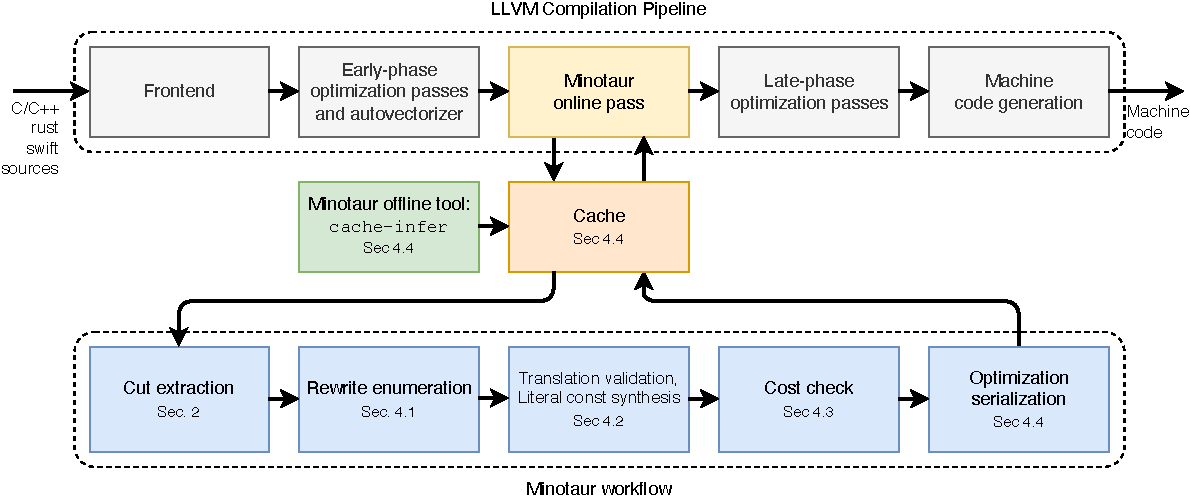
\includegraphics[width=\linewidth]{figures/flowchart.pdf}
    \caption{Overview of how \minotaur{} works, and how it fits into the
      LLVM optimization pipeline}
    \label{fig:workflow}
\end{figure}

Figure~\ref{fig:workflow} illustrates \minotaur's high-level structure,
and how it fits into LLVM\@.
%
It works by extracting many different \textit{cuts} from an LLVM function.
%
Each cut serves as the specification for a program synthesis
problem, where the objective is to synthesize a new cut that refines
the old one and is cheaper.
%
When such a cut is found, \minotaur{} uses it to rewrite the original
LLVM function, and also caches the rewrite.


Reasoning about the correctness of optimizations at the level of LLVM
IR can be very difficult; we have repurposed Alive2~\cite{alive2} to
serve as a verification backend.
%
To Alive2, we added formal semantics for Intel-architecture-specific
SIMD intrinsics.
%
Reasoning about the relative costs of code sequences is another
difficult problem; the solution adopted by \minotaur{} is to reuse the
LLVM Machine Code Analyzer~\cite{llvmmca}, which has adequately
accurate pipeline models for various modern processors.
%
These tools, along with the LLVM compiler itself, form the
foundation upon which \minotaur{} is built.


\textbf{Research contributions:}
%
First, we designed and implemented a domain-specific program
transformer that extracts an SSA value from an LLVM function, along
with context about how that value was computed.
%
Extracting enough context to permit interesting optimizations, without
extracting so much context that the underlying SMT solver was
overwhelmed, was an interesting empirical problem.
%
Second, we created a synthesis engine that searches for cheaper code
sequences; it enumerates partially symbolic candidates where the
instructions are concrete, but constants are symbolic.
%
For this part of our work, we created formal semantics for 165 LLVM
intrinsic functions that correspond to SIMD operations supported by
x86-64 processors, and added these to Alive2.
%
We also modified Alive2 to support synthesis of literal constants.
%
Third, to mitigate the large performance overhead of running program
synthesis at compile time, we developed infrastructure for caching
optimizations.
%
Thus, while \minotaur{} can be hundreds of times slower than \texttt{clang
  -O3} when its cache is cold, with a warm cache it is just 3\%
slower, when building the SPEC CPU 2017 benchmarks.



We performed a detailed evaluation of \minotaur's ability to speed up
code, showing that it can find numerous optimizations that LLVM fails
to perform, and also that it can achieve speedups on a variety of
real-world libraries and benchmarks.
%
\minotaur{} is also useful for compiler developers, and in fact several
optimizations it has discovered have now been implemented in upstream
LLVM\@.

\section{Cutting LLVM Functions}
\label{sec:cut}

Using a typical function in LLVM IR as the specification, it is not
practical to directly synthesize an optimized version of that
function.
%
The state of the art in program synthesis simply does not scale up to
the size of LLVM functions found in the wild.
%
Instead, \minotaur{} takes a divide-and-conquer approach: we individually
attempt to optimize each instruction in an LLVM function by extracting
a \textit{cut}---a subset of that instruction's dependencies.
%
If this cut of LLVM instructions can be optimized by program synthesis
then, by the compositionality of refinement, so can the original LLVM
function.
%
The rest of this section describes this process in more detail.


\subsection{Problem Statement}

Given a function $F$, an instruction $I$ within $F$, and a depth
bound $B$, our goal is to create a new LLVM function $C$ that:
%
\begin{enumerate}
\item
  is loop-free,
\item
  returns the value computed by $I$, and
\item
  contains every instruction in $F$ that can be reached by following
  up to $B$ backwards data, control, and memory dependency edges.
\end{enumerate}
%
Informally, we can think of $C$ as summarizing a subcomputation in
$F$, that is (hopefully) tractable for an SMT solver to reason about.


When an instruction is part of $C$ but its inputs are not, then these
become free inputs---these are implemented by adding them as
parameters to $C$.
%
We can think of every instruction that is not part of the cut as being
part of a residual function $R$.
%
However, note that \minotaur{} does not explicitly construct $R$---it
computes and optimizes $C$, and then applies the discovered
optimization, if any, directly to $F$ using a rewrite mechanism
described in Section~\ref{sec:rewrite}.


\subsection{Example}

\begin{figure}
  \centering
  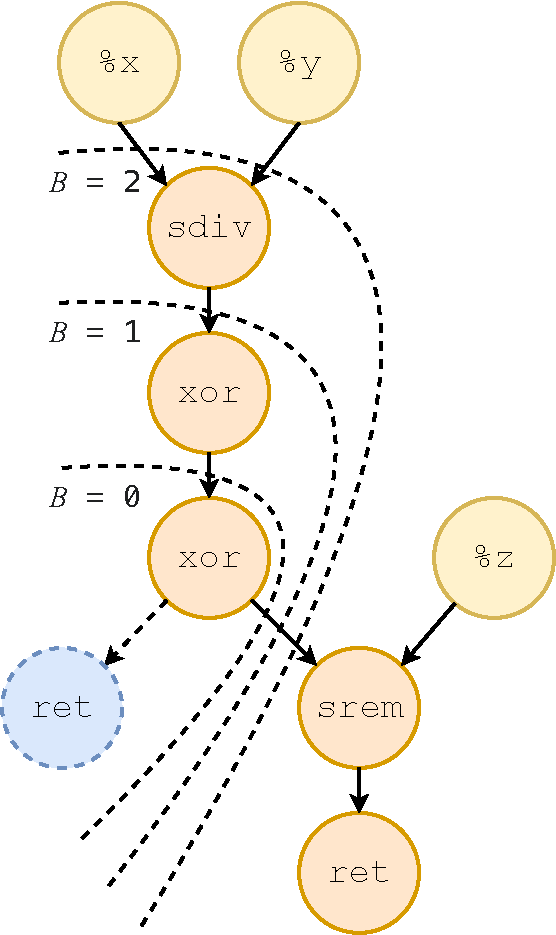
\includegraphics[width=0.5\linewidth]{figures/cut-depth.pdf}
  \caption{Example of cutting an LLVM function}
  \label{fig:cut-depth}
\end{figure}

Consider this LLVM function that takes three 64-bit arguments and
returns a 64-bit value, where \texttt{sdiv} is signed integer division
and \texttt{srem} is the signed integer modulus operator:

%%% https://gcc.godbolt.org/z/Wes9sPKGW

{\small\begin{quote}
\begin{verbatim}
define i64 @f(i64 %x, i64 %y, i64 %z) {
  %a = sdiv i64 %x, %y
  %b = xor i64 %a, -1
  %c = xor i64 %b, -1
  %d = srem i64 %c, %z
  ret i64 %d
}
\end{verbatim}
\end{quote}}

Figure~\ref{fig:cut-depth} illustrates various cuts of this function.
%
If we cut this function with respect to \texttt{\%c} with $B = 0$ then
we get the following decomposition (however, again, please bear in
mind that \minotaur{} does not actually construct $R$---we show it here to
make the explanation concrete):

\begin{multicols}{2}
{\small\begin{quote}
\begin{verbatim}
define i64 @r0(i64 %x, i64 %y, i64 %z) {
  %m = sdiv i64 %x, %y
  %n = xor i64 %m, -1
  %o = call i64 %c0(i64 %n)
  %p = srem i64 %o, %z
  ret i64 %p
}
\end{verbatim}
\end{quote}}
\columnbreak
{\small\begin{quote}
\begin{verbatim}
define i64 @c0(i64 %t1) {
  %t2 = xor i64 %t1, -1
  ret i64 %t2
}
\end{verbatim}
\end{quote}}
\end{multicols}

This is not useful, the cut \texttt{c0} contains too little context
to support any optimizations.
%
If we cut \texttt{f} with respect to \texttt{\%c} with $B = 1$ then we get:

\begin{multicols}{2}
{\small\begin{quote}
\begin{verbatim}
define i64 @r1(i64 %x, i64 %y, i64 %z) {
  %m = sdiv i64 %x, %y
  %o = call i64 @c1(i64 %m)
  %p = srem i64 %o, %z
  ret i64 %p
}
\end{verbatim}
\end{quote}}
\columnbreak
{\small\begin{quote}
\begin{verbatim}
define i64 @c1(i64 %t1) {
  %t2 = xor i64 %t1, -1
  %t3 = xor i64 %t2, -1
  ret i64 %t3
}
\end{verbatim}
\end{quote}}
\end{multicols}

This decomposition is useful: \texttt{c1} can be optimized to simply
return its argument.
%
If we increase the depth bound to two, then we would get:

\begin{multicols}{2}
{\small\begin{quote}
\begin{verbatim}
define i64 @r2(i64 %x, i64 %y, i64 %z) {
  %o = call i64 @c2(i64 %x, i64 %y)
  %p = srem i64 %o, %z
  ret i64 %p
}
\end{verbatim}
\end{quote}}
\columnbreak
{\small\begin{quote}
\begin{verbatim}
define i64 @c2(i64 %t1, i64 %t2) {
  %t3 = sdiv i64 %t1, %t2
  %t4 = xor i64 %t3, -1
  %t5 = xor i64 %t4, -1
  ret i64 %t5
}
\end{verbatim}
\end{quote}}
\end{multicols}

Here the cut \texttt{c2} can again be optimized (it can just return
\texttt{\%t3}), but now the solver must reason about a 64-bit signed
division---operations like this are difficult and frequently lead to
timeouts.
%
Choosing an appropriate depth bound is an empirical problem that
we address in Section~\ref{sec:loops}.


\subsection{Correctness Argument}

The composition of $R$ and $C$ is equivalent to the original function:
$F = R \circ C$.
%
In other words, the decomposition of $F$ into $R$ and $C$ preserves
the behavior of the original function---the difference is simply that
some dependency edges that were previously internal to $F$ now cross
the boundary between $R$ and $C$.


Next, if \minotaur{} can synthesize $C'$, an optimized function that
refines $C$, then we can compose that with the residual function to
get a new function $F' = R \circ C'$.
%
Since refinement is compositional, it follows that $F'$ refines $F$,
which is the property that we need for \minotaur{} to be a correct
optimizer.
%
The details of establishing a refinement relation between functions in
LLVM IR were presented by Lopes et al.~\cite{alive2}.


Alive2 is intended to be a sound refinement checker for LLVM
IR for LLVM functions that do not contain loops.
%
We avoid this potential unsoundness by ensuring that $C$ is loop-free,
in which case $C'$ is also loop-free since \minotaur{} never synthesizes a
loop.



\begin{algorithm}[tbp]
  \caption{Cut Extraction Algorithm}
  \begin{algorithmic}[1]
  \Function{ExtractCut}{\emph{F}: Function, \emph{I}: Instruction, \emph{B}: $\mathbb{N}$}
  \If{$I$ is in a loop}
    \State {\emph{AllowedBasicBlocks} $\gets $ all basic blocks in \emph{I}'s loop (innermost loop if nested)}
  \Else
    \State {\emph{AllowedBasicBlocks} $\gets$ all basic blocks in \emph{F} that is not in a loop}
  \EndIf
  \State {\emph{Harvested} $\gets \emptyset $}
  \State {\emph{Unknown} $\gets \emptyset $}
  \State {\emph{Visited} $\gets \emptyset $}
  \State {\emph{WorkList} $\gets$ \{ (\emph{I}, 0) \}}
  \While{\emph{WorkList} is not empty}
  \Comment{stage 1, instruction extraction}
  \State {(\emph{WI}, \emph{Depth}) $\gets $ \emph{WorkList}.pop()}
  \If {\emph{WI} $\in$ \emph{Visited}}
  \State \textbf{continue}
  \EndIf
  \State {Insert \emph{WI} into \emph{Visited}}
  \If{\emph{Depth} $>$ \emph{B}}
  \State {Insert \emph{WI} into \emph{Unknown}}
  \State {\textbf{continue}}
  \EndIf
  \If{\emph{WI} is not supported}
  \State {Insert \emph{WI} into \emph{Unknown}}
  \State {\textbf{continue}}
  \EndIf
  \State {\emph{BB} $\gets$ \emph{WI}'s basic block}
  \If{\emph{BB} $\notin$ \emph{AllowedBasicBlocks}} %$L$ $\land$ WI is not in $I$'s innermost loop}
  \State {Insert \emph{WI} into \emph{Unknown}}
  \State {\textbf{continue}}
  \EndIf
  \State {Insert \emph{WI} into \emph{Harvested}}
  \If{\emph{WI} is a Load instruction}
    \State {\emph{M} $\gets$ \emph{WI}'s linked \texttt{MemoryPhi} or \texttt{MemoryDef}}
    \If {\emph{M} is a \texttt{MemoryDef} $\wedge$ \emph{M} is a store}
    \State {\emph{MI} $\gets$ \emph{M}'s stored value}
    \State {Push (\emph{MI}, \emph{Depth} + 1) into \emph{WorkList} }
  \EndIf

  \Else
    \ForAll{operand \emph{Op} in \emph{WI}}
    \State {Push (\emph{Op}, \emph{Depth} + 1) into \emph{WorkList} }

    \EndFor
  \EndIf

  \State {\emph{T} $ \gets$ terminator of \emph{WI}'s basic block}
    \If {\emph{T} is a conditional branch instruction}
    \State {\emph{TI} $\gets$ \emph{T}'s condition value}
    \State {Push (\emph{TI}, \emph{Depth} + 1) into \emph{WorkList} }
    \EndIf

  \EndWhile
  \State {Insert every terminator instruction in \emph{F} to \emph{Harvested}}
  \State {Clone \emph{F} into \emph{C}}
  \Comment{stage 2, construct a loop-free LLVM function}
  \State {Delete instructions in \emph{C} except those in \emph{Harvested}}
  \State {Delete all back-edges in \emph{C}}
  \State {Add values in \emph{Unknown} to \emph{C} as function arguments}
  \State {Create return instruction for \emph{I} in \emph{C}}
  \State {\textbf{return} \emph{C}}
  \EndFunction
  \end{algorithmic}
  \label{alg:slicing}
\end{algorithm}


\subsection{Detailed Solution}

Algorithm~\ref{alg:slicing} shows the procedure that \minotaur{} uses to
extract a cut.
%
It works in two stages.
%
In the first stage, \minotaur{} determines which instructions will be part
of the cut, using a depth-bounded depth-first search.
%
During the search, two sets, \emph{Harvest} and \emph{Unknown}, are
propagated which will be used in the second stage for constructing the
cut.
%
\minotaur{} uses LLVM's LoopInfo pass~\cite{loopinfo} to identify loops in the
source function.
%
If instruction $I$ is in a loop, \minotaur{} will only extract
instructions that are defined inside the loop.
If the loop is nested, \minotaur{} will only extract instructions that are
defined inside the innermost loop.
\minotaur{} will give up if the loop is irregular.
%
If $I$ is not in a loop, \minotaur{} will skip the instructions that are in a loop.
%
\minotaur{} marks non-intrinsic function calls, operations on global
variables, and operations that are not recognized by Alive2 as
unsupported.
%
All unsupported operations, operations that are beyond the depth
limit, and operations that are outside the loop are discarded and
replaced with free inputs.


For each conditional branch instruction, \minotaur{} extracts the branch
condition, since these carry control flow information that is useful
during synthesis.
%
Similarly, when it extracts a load from memory, \minotaur{} consults
LLVM's MemorySSA pass~\cite{MemorySSA} to get a list of stores that
potentially influence the loaded value.
%
MemorySSA marks memory operations with one of the three memory access tags:
\texttt{MemoryDef}, \texttt{MemoryUse}, and \texttt{MemoryPhi}.
Each memory operation is associated with a version of memory state.
%
A \texttt{MemoryDef} can be a store, a memory fence, or any operation
that creates a new version of the memory state.
%
A \texttt{MemoryPhi} combines multiple \texttt{MemoryDef}s when
control flow edges merge.
%
A \texttt{MemoryUse} is a memory instruction that does not modify
memory, it only reads the memory state created by \texttt{MemoryDef}
or \texttt{MemoryPhi}; a load instruction is always a
\texttt{MemoryUse}.
%
Because it must overapproximate, \minotaur{} is conservative when finding
the load-affecting store: it starts from the loads
\texttt{MemoryUse}'s memory version and walks along the MemorySSA's
def-use chain,
%
and when the associated memory operation is a \texttt{MemoryDef}, it
checks if the operation is a store and pushes the stored value into
the worklist.
%
\minotaur{} gives up when the associated memory version is tagged with
\texttt{MemoryPhi}, or when the version is tagged with
\texttt{MemoryDef} but the operation is not a store instruction.


In the second stage, \minotaur{} builds the extracted function; it does
this by cloning the original function and then deleting all
instructions that are not in the cut.
%
\minotaur{} then deletes all the loop backedges so that the extracted
function is loop-free.
%
Finally, a return instruction is added to return the value computed by
the instruction that is the basis for the cut.

\begin{figure}
  \centering
  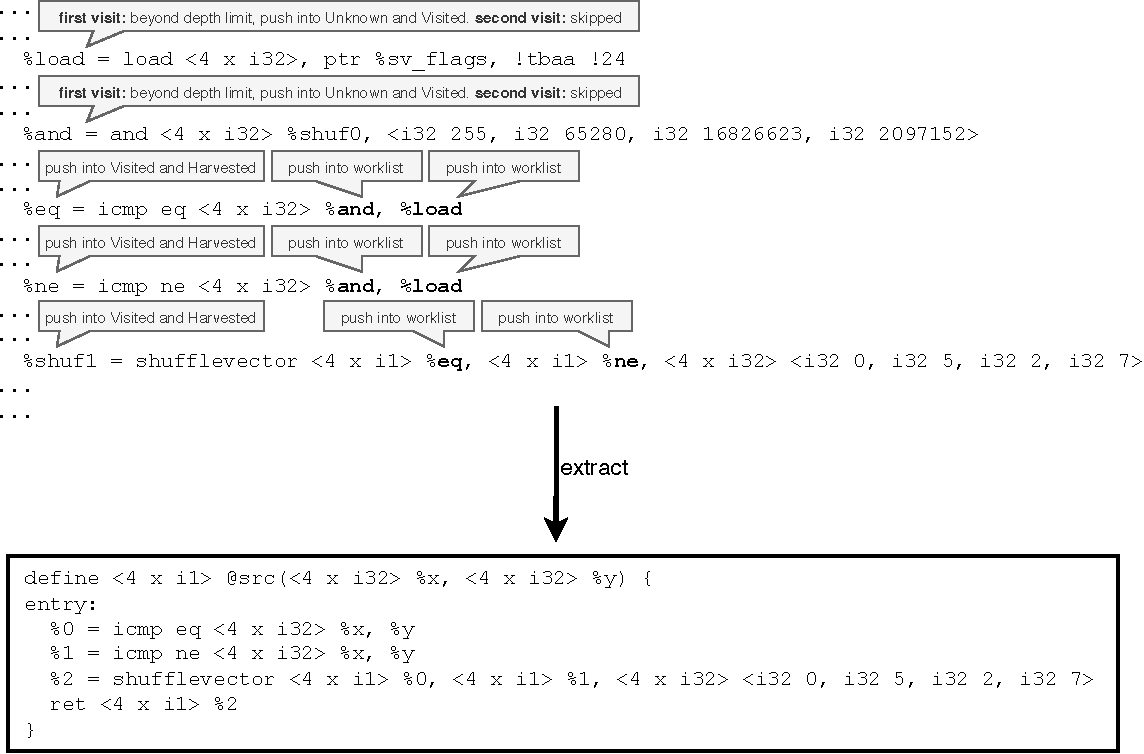
\includegraphics[width=\linewidth]{figures/slice.pdf}
  \caption{Example of cut extraction}
  \label{fig:cut}
\end{figure}


Figure~\ref{fig:cut} shows an example of cut extraction
for value \texttt{\%shuf1}.
%
The cutting algorithm starts on \texttt{\%shuf1} and walks along the
def-use chain to extract the instructions that are involved in the
computation of \texttt{\%shuf1}.
%
A new function is created to hold the extracted instructions shown
in the bottom of the figure.



\subsection{Relation to Previous Cut-Based Superoptimizers}

\minotaur's cut extraction algorithm is fundamentally more aggressive
than Bansal and Aiken's approach~\cite{Bansal06}, which extracted a
small window of sequential instructions.
%
It is also considerably more aggressive than Souper~\cite{souper},
which had a very limited view of control flow and refused to consider
memory operations, vector operations, and floating-point operations.
\section{Synthesizing Optimizations}

For every cut extracted from an LLVM function, \minotaur{}'s goal is to
synthesize a cheaper way to compute the value returned by that cut.
%
It does this by enumerating \emph{candidates}---code fragments that
potentially refine the current cut.
%
When a candidate is found that refines the original cut, \minotaur{}
consults a cost model.
%
If the new code is cheaper than the original cut, \minotaur{} applies the
rewrite to the function that is being optimized.

\subsection{Designing an Appropriate Synthesis Procedure}

A delicate part of designing a practical program synthesis algorithm
is determining how much of the search is pushed to the solver, and how
much searching gets done by code outside the solver.
%
At one extreme, as the Denali paper~\cite{denali02} points out, we
could simply give the SMT solver a conjecture of the form ``No program
of the target architecture computes P in at most eight cycles.''
%
If the solver can disprove this conjecture, then its counterexample
will tell us how to compute P in eight or fewer cycles.
%
This kind of query is asking the solver to do all of the work of
finding a program that disproves the conjecture, including reasoning
about the costs of various alternatives, in a single, complicated
query---this is very heavy lifting.
%
At the other extreme, we could enumerate completely concrete
candidates, and use the SMT solver only to perform the necessary
refinement checks.
%
The problem with this approach is literal constants: even a single
64-bit constant in the synthesized code will require us to enumerate
and check $2^{64}$ alternatives; this is clearly infeasible.


We spent a considerable amount of time investigating different points
between these extremes, and finally settled on a design that makes
things as easy as possible for the solver, but without exploring all
possible choices of values for literal constants.
%
\minotaur{} creates \emph{partially symbolic} candidates where
instructions are represented concretely, but constants are symbolic.
%
This gives a reasonably tractable enumeration space without giving up
synthesis power.
%
Our rationale for this design is that, based on extensive experience
with LLVM and Alive2, a lot of individual refinement checks that we
want to perform---especially those that contain multiplications,
divisions, floating point operations, and pointer indirections---are
already very difficult.


\subsection{Synthesis in Minotaur}

\begin{table}[tbp]
  \centering
  \caption{Operations that \minotaur{} can synthesize}
  \begin{tabular}{ r | l }
    \textbf{Operation Type} & \textbf{Instructions} \\
    \hline
    Unary integer & ctpop, ctlz, cttz, bitreverse, bswap \\
    Unary FP & fneg, fabs, fceil, ffloor, frint, fround, fnearbyint, froundeven \\
    Binary integer & add, sub, mul, udiv, sdiv, umax, umin, smax, smin\\
    Binary FP & fadd, fsub, fmul, fdiv, frem, fmaximum, fminimum, ... \\
    Bitwise & and, or, xor, shl, lshr, ashr \\
    Comparison & icmp, fcmp, select \\
    Conversion & zext, sext, trunc, fptrunc, fpext, fptosi, sitofp, fptoui, uitofp \\
    Data movement & extractelement, insertelement, shufflevector \\
    SIMD intrinsics & 165 vector intrinsics mapping to intel vector instructions \\
  \end{tabular}
  \label{tab:operations}
\end{table}

\begin{algorithm}[tbp]
  \caption{Minotaur's Synthesis Procedure}
  \label{alg:enumerate}
  \begin{algorithmic}[1]
  \Function{SynthesizeRefinements}{Cut: Function, InstLimit: $\mathbb{N}$, TimeLimit: $\mathbb{N}$}
  \\
  \Comment {Phase 1: Populate the instruction pool}

  \State {Inputs $\gets$ all the SSA definitions in Cut}
  \State{InstPool $\gets \emptyset$}
  \ForAll {op in binary operations listed in Table~\ref{tab:operations}}
    \State {InstPool $\gets$ InstPool $\cup$ \{ (op hole, hole), (op sym-const, hole), (op hole, sym-const) \} }
    \ForAll {input1 in Inputs}
      \State {InstPool $\gets$ InstPool $\cup$ \{ (op input1, sym-const), (op sym-const, input1) \}}
      \State {InstPool $\gets$ InstPool $\cup$ \{ (op input1, hole), (op hole, input1) \}}
      \ForAll {input2 in Inputs}
        \State {InstPool $\gets$ InstPool $\cup$ \{ (op input1, input2) \}}
      \EndFor
    \EndFor
  \EndFor

  \ForAll {other operations in Table~\ref{tab:operations}}
  \Comment{omitted for brevity}
    \State {...}
  \EndFor

  \\
  \\
  \Comment{Phase 2: Generate partially-symbolic candidates}

  \State {WorkList $\gets$ \{ (ret hole), (ret sym-const) \} }

  \State {Candidates $\gets$ Inputs}

  \While {WorkList $\neq \emptyset$}
    \State {I $\gets$ WorkList.pop()}

    \If {I does not contain holes}
      \State {Candidates $\gets$ Candidates $\cup$ \{ I \}}
      \State{\textbf{continue}}
    \EndIf

    \ForAll {Hole in I}
      \If {CountNewInsts(I) $\geq$ InstLimit}
        \State{\textbf{continue}}
      \EndIf
      \ForAll {Inst in InstPool}
        \State {J $\gets$ I with Hole substituted by Inst}
          \If {TargetTransformInfoCost(J) $\geq$ TargetTransformInfoCost(Cut)}
            \State{\textbf{continue}}
          \EndIf

          \State {WorkList $\gets$ WorkList $\cup$ \{ J \}}
      \EndFor
    \EndFor

  \EndWhile

  \\
  \\
  \Comment{Phase 3: Refinement checking and constant synthesis}
  \State {Sort Candidates by TargetTransformInfoCost}
  \State {StartTime $\gets$ time()}
  \State {Refinements $\gets \emptyset$}

  \ForAll {C in Candidates}
    \If {C does not contain symbolic constants}
      \If {Alive2 claims that C refines Cut}
        \State {Refinements $\gets$ Refinements $\cup$ \{ C \}}
      \EndIf
    \Else
      \State {Build exists-forall query to get a model for symbolic constants}
      \If {satisfiable}
        \State {C' $\gets$ C with symbolic constants substituted by the constants in the model}
        \State {Refinements $\gets$ Refinements $\cup$ \{ C' \}}
      \EndIf
    \EndIf
    \If {time() - StartTime $\geq$ TimeLimit}
      \State{\textbf{break}}
    \EndIf
  \EndFor

  \State{\textbf{return} Refinements}

  \EndFunction
  % \State{\{ Complete, Incomplete \} $\gets$ \textsc{GenerateSingleInstruction}(Inputs)}
  % \State {WiredInsts $\gets$ Put Complete and Incomplete into the each of holes in Inst}
  \end{algorithmic}
  \label{alg:synthesis}
\end{algorithm}

Algorithm~\ref{alg:synthesis} describes \minotaur's synthesis procedure.
%
In Phase~1, it creates a pool of instructions whose operands are
selected from the available SSA values in the current cut (a dominance
check is not required since cuts are constructed in such a way that
every existing SSA definition dominates the synthesized portion of the
function), from symbolic constants, and from \emph{holes} that
represent instructions that have not yet been enumerated.
%
The list of instructions that \minotaur{} can synthesize is shown in
Table~\ref{tab:operations}.
%
The description in Algorithm~\ref{alg:synthesis} only shows the case
for instructions taking two operands, and it also omits a number of
simple pruning strategies that are useful in practice, such as
avoiding enumeration of redundant versions of commutative operations.
%
In Phase~2 of the synthesis procedure, instructions from the pool are
used to recursively fill holes; this procedure terminates when all
holes are filled (in which case a complete candidate has been
generated) or when at least one hole remains, but there is no remaining
instruction budget to fill it (in which case the incomplete candidate
is discarded).
%
A subtlety here is that
LLVM's \texttt{bitcast} instruction, which changes the type
of an SSA value without changing its representation, does not count
towards the instruction limit.
%
This is because \minotaur{} takes a low-level, untyped view of values.
%
For example, it internally treats a 16-way vector of 8-bit values the
same as an 8-way vector of 16-bit values: both of these are simply
128-bit quantities.
%
This lack of type enforcement allows \minotaur{} to find interesting,
low-level optimizations such as those that use bitwise operations to
rapidly perform certain floating point operations.


\begin {figure}[tbp]
  \centering
  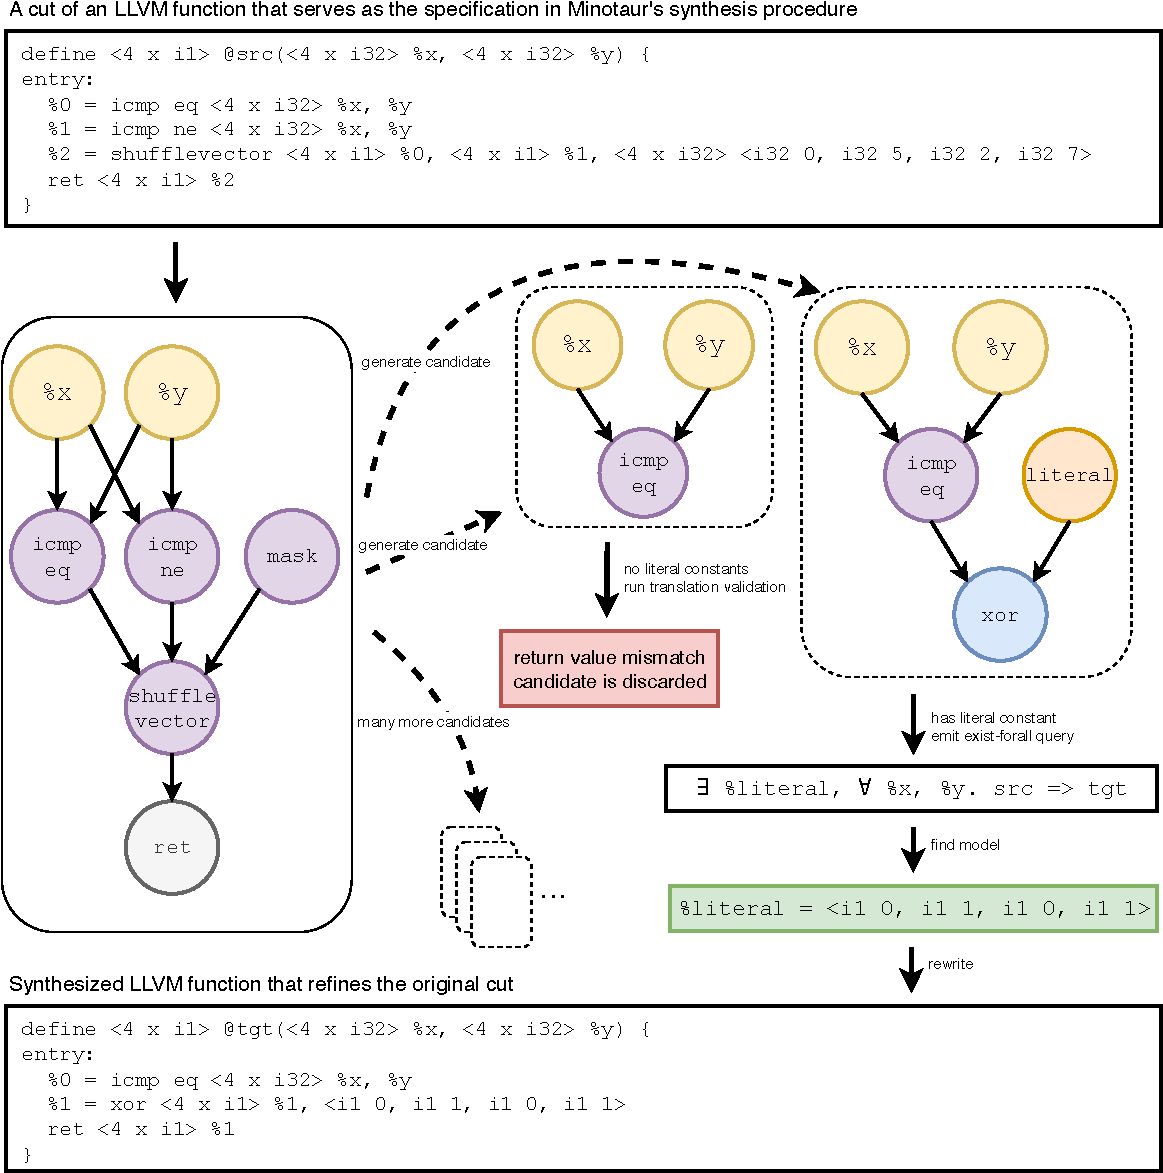
\includegraphics[width=0.8\linewidth]{figures/solve_literal.pdf}
  \caption{Example of synthesizing a rewrite that contains literal constants}
  \label{fig:synthesizing}
\end{figure}

In Phase~3 of Algorithm~\ref{alg:synthesis}, \minotaur{} uses Alive2 to
eliminate every candidate that does not refine the specification.
%
First, we sort the candidates in order of increasing cost using LLVM's
TargetTransformInfo~\cite{tti}: a cost model that roughly captures
execution cost on the target, and is cheap to compute.
%
We do this to ensure that likely-beneficial rewrites are tested first,
before the synthesis time limit is reached.
%
For candidates that do not contain symbolic constants, we can use
Alive2 as-is.
%
To support symbolic constants, we modified Alive2 to wrap
its refinement check in an exists-forall query.
%
In other words, \minotaur{} asks the question: ``Does there exist a
valuation of the symbolic constants such that the synthesis candidate
refines the specification for all possible values of the inputs?''
%
When such a query is satisfiable, the model returned by the solver can
be inspected to find satisfying values of the symbolic constants
in the candidate, which now become literal constants, giving a
complete, sound optimization.
%
To avoid potentially-expensive exists-forall queries, we experimented
with various techniques such as generalization by
substitution~\cite{Dutertre15}.
%
However, these failed to outperform exists-forall queries, in the
version of Z3 that we used (4.12.4).
%
Figure~\ref{fig:synthesizing} illustrates \minotaur's synthesis procedure.


\subsection{Identifying Profitable Rewrites}

The output of Algorithm~\ref{alg:synthesis} is a list of candidates
that all refine the cut.
%
Of these, we want to choose the best one---but predicting throughput
of code running on modern microprocessors is not straightforward.
%
We leverage the LLVM Machine Code Analyzer (LLVM-MCA)~\cite{llvmmca},
which was created to help developers improve performance-critical
code.
%
It is an interactive tool that emits a graphical depiction of pipeline
behavior, but its functionality can also be accessed programmatically,
and this is what \minotaur{} does, after lowering each candidate to
x86-64 object code.
%
Then, \minotaur{} only applies a rewrite if its estimated cost, using
LLVM-MCA, is lower than that of the original cut, and lower than
that of any other synthesized refinement of the original cut.


Although LLVM-MCA can estimate the cycle cost of LLVM functions, we
instead use the number of uOps (``micro-operations,'' a modern x86-64
processor's internal instruction set) as the estimated cost.
%
This choice was driven by empirical data: after extensive
experimentation, we determined that, for our purposes, uOps are a
better performance predictor than cycles.



\subsection{Representing and Caching Rewrites}
\label{sec:rewrite}

\minotaur{} stores each potential rewrite as a pair: $(C, S)$
where $C$ is a cut, represented by a function in LLVM
Intermediate Representation (IR), and $S$ is a rewrite description---an
expression in \minotaur's own intermediate representation that describes a
different way to compute the return value of $C$.
%
Rewrite descriptions are directed acyclic graphs containing nodes that represent
operations, and edges representing data flow.
%
Although the elements found in \minotaur{} IR are similar to those found
in LLVM IR, we could not reuse LLVM IR to represent rewrites since
LLVM IR does not support incomplete code fragments, and also rewrites
must contain enough information to support connecting the new code in
the rewrite to code in the unoptimized function.


To support caching, rewrites must be serializable.
%
The cut $C$ can be serialized using existing LLVM functionality, and we
created a simple S-expression syntax for serializing the $S$ part.
%
Figure~\ref{fig:syntax} shows the syntax of the IR\@.
%
For example, if the returning value of $C$, a 32-bit instruction is
replaced by left shift by one bit position, the textual format for
the expression is \texttt{(shl (val i32 \%0), (const i32 1), i32)}.


Rewrites are cached in a Redis instance: this implementation choice
allows the cache to be persistent across multiple \minotaur{} runs and
also makes the cache network-accessible.
%
Synthesis can be done online---during compilation---but also
offline, in a mode where \minotaur{} extracts cuts into the Redis
cache but does not perform synthesis.
%
In this mode, compilation is only slowed down by a few percent.
%
\minotaur's offline mode is designed for batch processing.
%
In this mode, a separate program called \texttt{cache-infer} retrieves
cuts from the cache, runs synthesis on them, and stores any
optimizations that it discovers back into the cache.
%
Unlike the online mode, which runs synthesis tasks one after the
other, offline mode can run all synthesis jobs in parallel.



\begin{figure}[tbp]
  \begin{tabular}{r c l}
    \emph{Op} &::=& \emph{Inst} | \emph{Constant} | \emph{Value} \\
    \emph{Inst}  &::=& (\emph{UnaryOp} \emph{Op}, \emph{Type}) | (\emph{BinaryOp} \emph{Op}, \emph{Op}, \emph{Type}) | (\emph{Conversion} \emph{Op}, \emph{Type}) |\\
              && (insertelement \emph{Op}, \emph{Op}, \emph{Op}) | (extractelement \emph{Op}, \emph{Op}) | (shufflevector \emph{Op}, \emph{Op}, \emph{Constant}) |\\
              && (\emph{Comparison} \emph{Op} \emph{Op}) | (select \emph{Op}, \emph{Op}, \emph{Op}) | (\emph{Intrinsic} \emph{Op}, \emph{Op}) \\
    \emph{Constant} &::=& (const \emph{Type} \texttt{number-literal}) \\
    \emph{Value} &::=& (val \emph{Type} \texttt{llvm-identifier}) \\

    \emph{Type} &::=& \emph{ScalarType} | <elements $\times$ \emph{ScalarType}> \\
    \emph{ScalarType} &::=& i1 | i8 | i16 | i32 | i64 | half | float | double | fp128 \\
    \emph{BinaryOp} &::=& xor | and | or | add | sub | mul | udiv | sdiv | ashr | lshr | shl | umax | umin | smax | smin\\
                && fadd | fsub | fmul | fdiv | copysign | fmaximum | fminimum | fmaxnum | fminnum \\
    \emph{UnaryOp} &::=& ctpop | ctlz | cttz | bswap | bitreverse | ret\\
                      && fneg | fabs | fceil | ffloor | frint | fround | ftrunc | fnearbyint | froundeven \\
    \emph{Conversion} &::=& zext | sext | trunc |\\
                    && fptrunc | fpext | fptosi | sitofp | fptoui | uitofp \\
    \emph{Comparison} &::=& eq | ne | ult | ule | slt | sle |\\
                && oeq | ogt | oge | olt | ole | one | ord | ueq | ugt | uge | ult | ule | une | uno \\
    \emph{Intrinsic} &::=& ssse3.phadd.d.128 | avx2.pavg.b | avx512.pmaddubs.w.512 | \dots (165 intrinsics in total) \\
  \end{tabular}
  \caption{Syntax for Minotaur rewrites}
  \label{fig:syntax}
  %\Description[syntax]{Minotaur syntax}
\end{figure}



\subsection{Integration with LLVM}

\minotaur{} is loaded into LLVM as a shared library where it runs as an
optimization pass.
%
We arranged for it to run at the end of LLVM's auto-vectorization pipeline.
%
We invoke LLVM's Dead Code Elimination pass after Minotaur to
clean up the resulting code.

\section{Evaluation}
\label{sec:evaluation}

This section evaluates \minotaur{}.


\subsection{Correctness}

Every optimization discovered by \minotaur{} has been formally verified by
Alive2.
%
Even so, bugs might remain in the instruction semantics that we have
added to Alive2, in our cut extractor, in our rewrite mechanism, or in
Alive2 itself.
%
To defend against implementation errors, we have compiled numerous
open source applications using \minotaur, and then run those applications'
test suites, to ensure that they were not miscompiled.
%
Furthermore, we have compiled SPEC CPU 2017 using \minotaur{} and
used the SPEC drivers to ensure that all of its benchmarks behave
as expected.


\subsection{Effect of Depth Bounds in the Cut Extractor}
\label{sec:loops}

%1345 loops are integer only + vectorizable
%plot only shows 879 loops, these are the loops touched by minotaur.

% 2386 loops are integer / fp + vectorizable
% depthlimit 5: 26339 exprs (305 opt), 290 source changed, 667 min elapsed
% depthlimit 4; 24334 exprs

% \begin{figure*}[tbp]
%   \centering
%   \subfloat[Targeting Intel Cascade Lake; geomean=1.061x\label{plot:loops-intel}]{
%     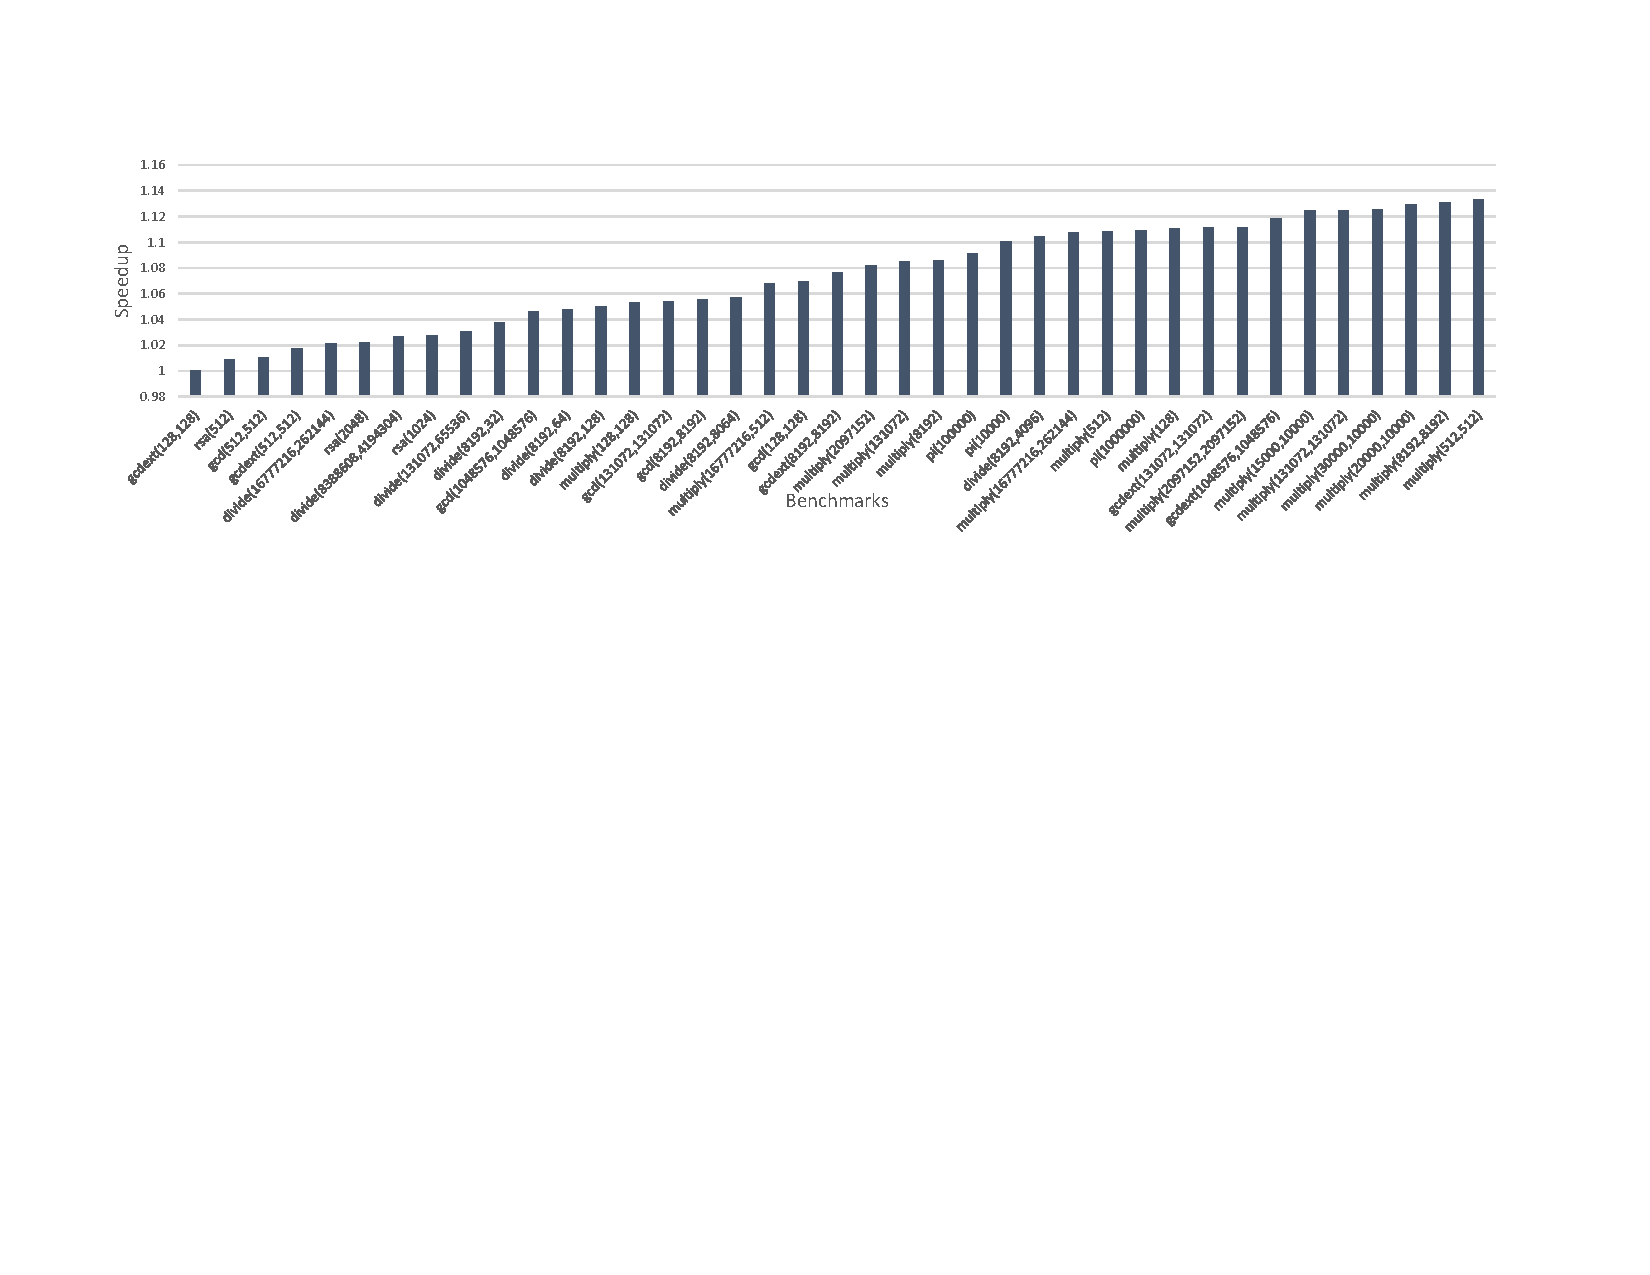
\includegraphics[page=1,width=\linewidth]{figures/data.pdf}
%   }`
%   \hfill'
%   \subfloat[Targeting AMD Zen 3; geomean=1.021x\label{plot:loops-amd}]{
%     \includegraphics[page=2,width=\linewidth]{figures/data.pdf}
%   }
%   \caption{Speedups---estimated by LLVM-MCA---due to running \minotaur{}
%     on a loop micro-benchmark suite}
% \end{figure*}

It is important for \minotaur{} to extract cuts that are of an appropriate
size.
%
If they are too large, compile times suffer and also the SMT solver
can be overwhelmed, leading to timeouts; if cuts are too small, then
they form an insufficient basis for driving an optimization.
%
To determine a good value for $B$, the depth parameter to the cut
extraction procedure shown in Algorithm~\ref{alg:slicing}, we
performed an empirical study.
%
We started with FlexC's benchmark suite~\cite{woodruff2023rewriting},
a collection of 2,386 compilable, non-trivial C functions containing
loops from FFMPEG, FreeImage, DarkNet, xz, bzip2, and the LivermoreC
benchmark.
% \footnote{The loop data set was provided
% by Alexander Brauckmann and Michael O'Boyle at the University of
% Edinburgh, UK\@.  At present, no citable reference for this work
% exists.}
%
When compiled to LLVM IR, these functions contain a total of 123,062
instructions; thus, our cut extractor was invoked 123,062 times for
each depth bound.
%
We chose this code as the basis for our experiment because it is
derived from real applications while also being small enough to
keep compile times manageable (compared to, e.g., SPEC CPU 2017,
which is much larger).


\begin{figure}[tbp]
  \centering
  \subfloat[Unique cuts extracted\label{fig:loop-expression}]{
    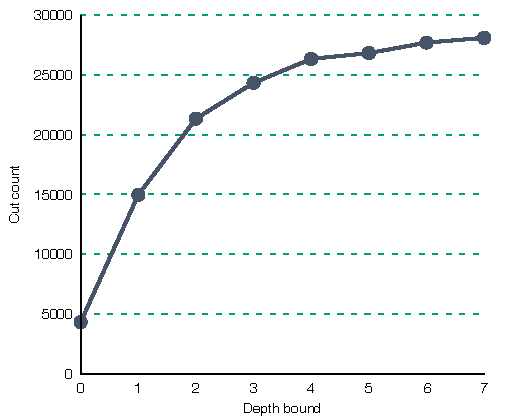
\includegraphics[width=0.32\linewidth]{figures/spec/expression-count.pdf}
  }
  \hfill
  \subfloat[Unique opts. synthesized\label{fig:loop-optimization}]{
    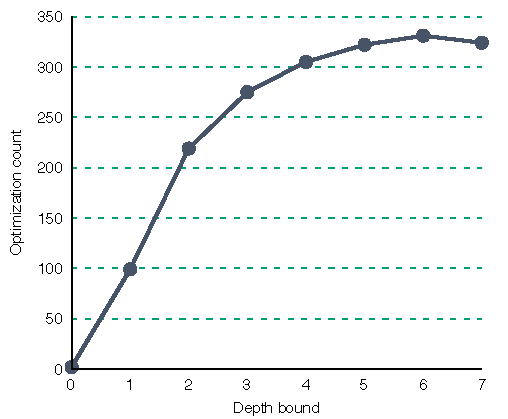
\includegraphics[width=0.32\linewidth]{figures/spec/optimization-count.pdf}
  }
  \hfill
  \subfloat[Compilation time\label{fig:loop-buildtime}]{
    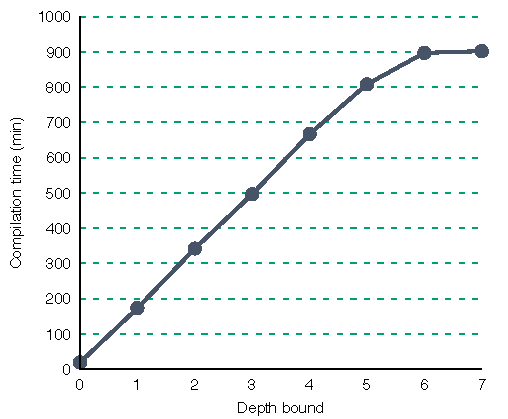
\includegraphics[width=0.32\linewidth]{figures/spec/compilation-time.pdf}
  }
  \caption{Evaluating the effect of varying $B$, the depth bound for
    cut extraction}
  \label{fig:loop}
\end{figure}


We then ran \minotaur{} on these functions with all depth bounds from
0--7, measuring the number of unique cuts that were extracted, the
number of optimizations found, and the compilation time.
%
We used a one-minute timeout for individual Z3 queries, and we also
gave \minotaur{} a total of up to five minutes to synthesize an optimized
version of each cut.
%
Figure~\ref{fig:loop} summarizes the results of this experiment.
%
The number of unique cuts that are extracted grows quickly with $B$,
but eventually begins to saturate simply because the functions being
compiled do not always have very long dependency chains.
%
The number of synthesized optimizations also grows quickly, but it
peaks when $B=6$ and then it decreases because the size of the cuts
causes many solver timeouts.
%
Finally, the total compile time increases smoothly with the depth
bound, eventually leveling off as most solver queries time out.


For the experiments in the rest of the evaluation section, we chose
$B=4$ because this gets pretty close to the maximum observed number of
optimizations without requiring exorbitant compile times.
%
It seems likely that there is room for improvement in this aspect of
\minotaur: perhaps the depth bound should be determined adaptively.
%
In this scenario, we would extract more and more components into the
cut, until either an optimization is found or else the solver begins
to time out.
%
We leave explorations of this nature for future work.


\subsection{Speedups for Benchmarks and Applications}

In this section, we show how \minotaur{} speeds up real-world benchmarks
and applications.

\paragraph{Experimental setup}
%
We used two machines for our evaluation: one with an Intel Xeon Gold
6210U processor running at 2.5\,GHz (this implements the Cascade Lake
microarchitecture~\cite{cascadelake}) and the other with an
AMD Ryzen 5950x processor
running at 3.4\,GHz (this implements the Zen~3 microarchitecture~\cite{zen3}).
The Intel machine supports the AVX-512 instruction set.
%
Both machines run Linux and were idle except for a single core running
our benchmarks.
%
To reduce the performance variation caused by frequency scaling, we
disabled turbo boost on the Intel machine and the core performance
boost on the AMD machine.
%
We invoked LLVM with the \texttt{-march=native} compilation flag to
ask it to take maximum advantage of processor features; we left other
compilation flags unchanged, except where noted.
%
All benchmarks are compiled at the \texttt{-O3} optimization level.
%
We set the timeout for Z3~\cite{z3} queries to one minute.
%
Finally, for each instruction that it tries to optimize, \minotaur{} gives
up if no solution is found within five minutes.


\paragraph{Benchmark selection}
%
We evaluate on SPEC CPU 2017%\footnote{\url{https://www.spec.org/cpu2017/}}
because it is a widely accepted standard
benchmark.
%
We only evaluate on the \emph{speed} subset of the SPEC suite, and we omit
648.exchange, 607.cactuBSSN, 621.wrf, 627.cam4, 628.pop2, 649.fotonik3d,
and 654.roms as they contain Fortran code.
%
We additionally use GMP, the GNU Multiple Precision Library, and libYUV,
which is used by Google Chrome/Chromium for manipulating images in the
YUV format.
%
We chose these libraries because they have been heavily tuned for
performance, they rely on loops, and they come with performance
benchmark suites that we could simply reuse.


\paragraph{Compile times}
%
Table~\ref{tab:compiletime} shows how long it takes \minotaur{} to process
our benchmarks, along with the number of potentially optimizable
values and the number of optimizations found.
%
In most cases, \minotaur{} found more optimizations when targeting the AMD
processor.
%
We believe this is because LLVM is more mature targeting
AVX2 than AVX512.
%
Solving queries with 256-bit vectors is also less likely to cause Z3
to timeout than are 512-bit vectors.
%
Minotaur is quite slow when it runs with a cold cache because it
performs a large number of solver queries.
%
However, with a warm cache, it is only 3\% slower than baseline \texttt{clang}.

\begin{table}[t]
  \centering
  \begin{tabular}{| r | r r  r | r r | r r r | r r |}
    \hline
    \multirow{2}{*}{}& \multicolumn{5}{c|}{Intel Cascade Lake} & \multicolumn{5}{c|}{AMD Zen3} \\
    \cline{2-11}
    & \multicolumn{3}{c|}{Compilation time (min)} & \multicolumn{2}{c|}{Opt. found} & \multicolumn{3}{c|}{Compilation time (min)} & \multicolumn{2}{c|}{Opt. found}  \\
    \hline
    Benchmarks & cold cache & warm & clang & \# cut & \# opt. & cold cache & warm & clang & \# cut & \# opt. \\
    \hline\hline
    SPEC CPU 2017 & 2,337 & 3 & 3 & 109,177 & 2,683 & 2,580 & 3 & 3 & 114,612 & 2,820 \\
    \hline
    gmp-6.2.1 & 440 & < 1 & < 1 & 9,170 & 336 & 445 & < 1 & < 1 & 9,265 & 387\\
    \hline
    libYUV & 2,196 & < 1 & < 1 & 6,849 & 334  & 2,193 & < 1 & < 1 & 6,809 & 357 \\
    % \hline
    % OpenBLAS-0.3.26 & 554 & < 1 & < 1 & 8,683 &  & 670 & < 1 & < 1 & 9,182 & 156 \\
    \hline
  \end{tabular}
  \caption{Compile-time statistics}
  \label{tab:compiletime}
\end{table}

\paragraph{Optimizing GMP with \minotaur{}}

\begin{figure}[tbp]
  \centering
  \subfloat[Speedups on Intel Cascade Lake, geomean = 1.073x\label{plot:gmp-intel}]{
    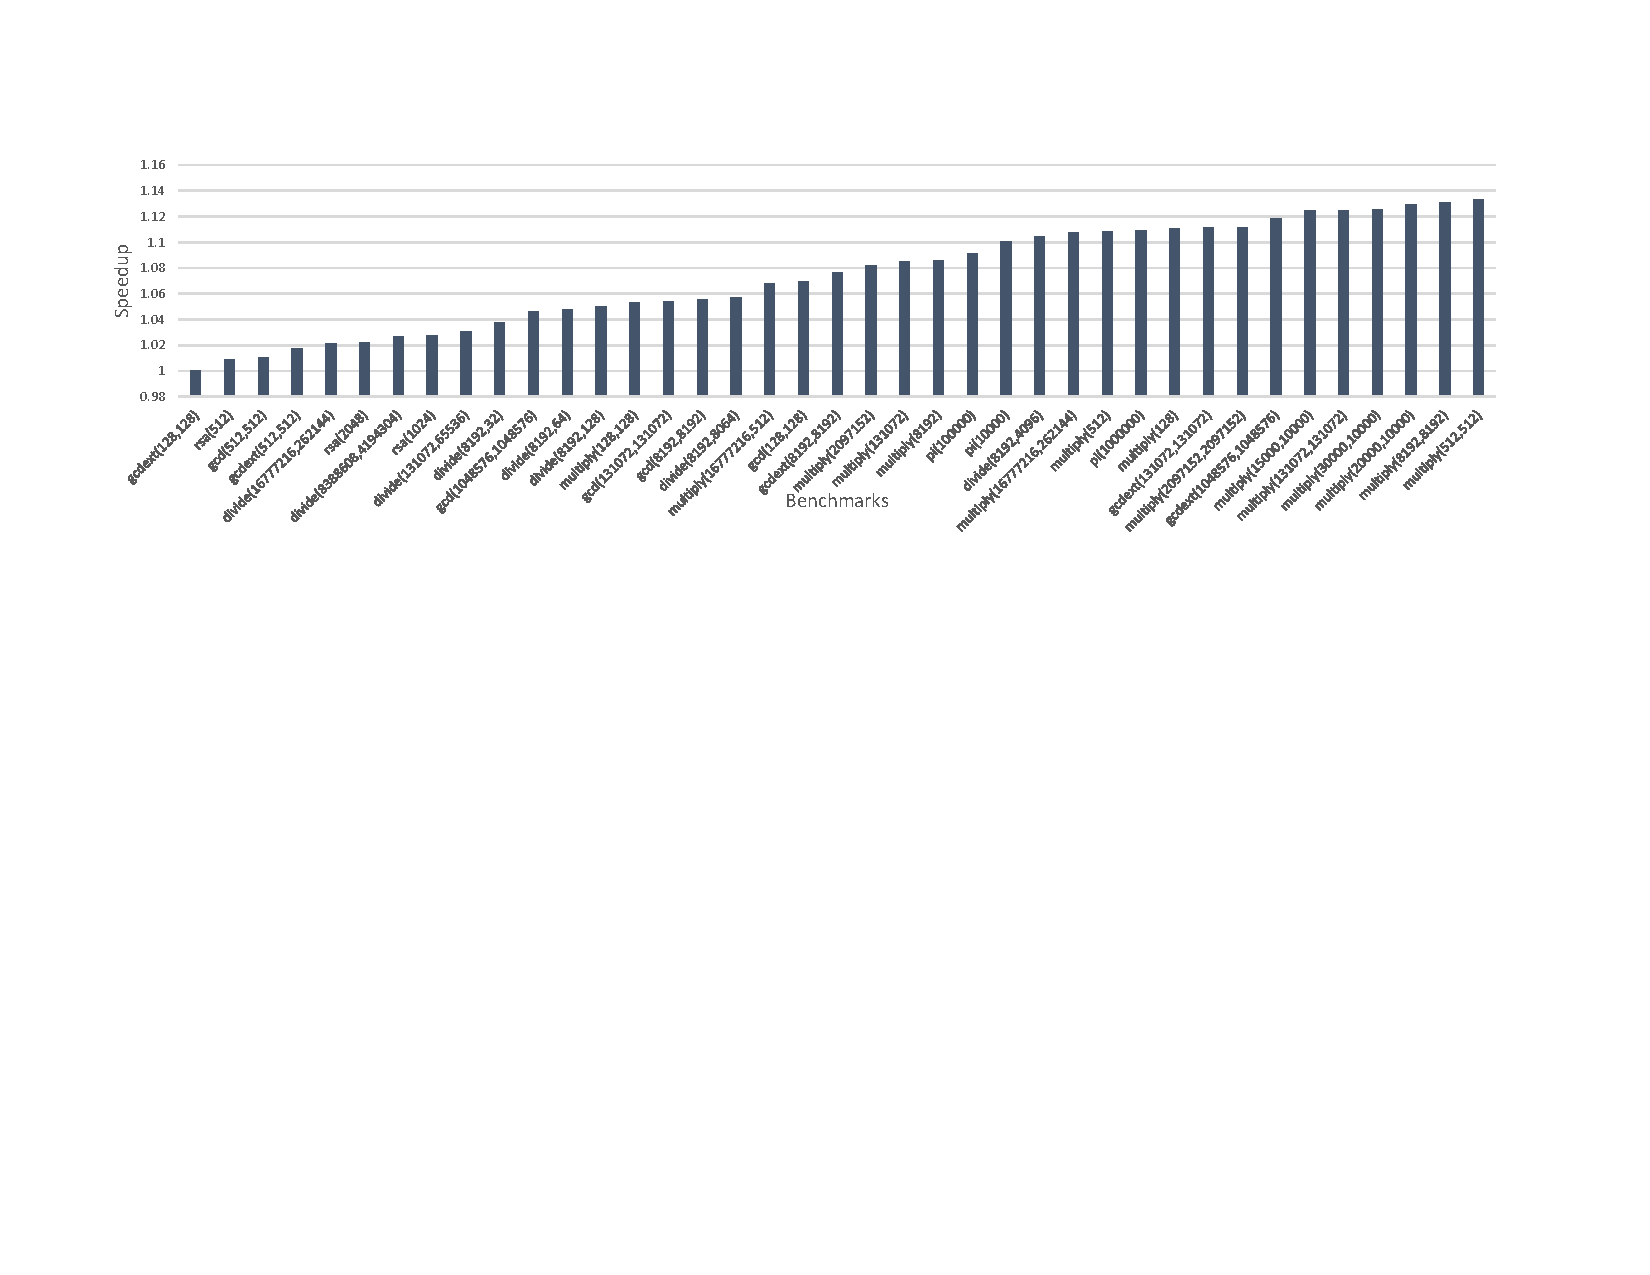
\includegraphics[page=1,width=\linewidth]{figures/data.pdf}
  }
  \hfill
  \subfloat[Speedups on AMD Zen 3, geomean = 1.065x\label{plot:gmp-amd}]{
    \includegraphics[page=2,width=\linewidth]{figures/data.pdf}
  }
  \caption{GNU Multiple Precision Library (GMP) speedups}
  \label{fig:gmp}
\end{figure}


GMP provides a portable C-language implementation and then, for
several platforms, a faster assembly language implementation.
%
For this evaluation, we selected the C implementation, because \minotaur{}
works on LLVM IR and cannot process assembly code at all.
%
The benchmark suite that we used is
GMPbench.%\footnote{\url{https://gmplib.org/gmpbench}}
%
Figure~\ref{fig:gmp} summarizes the results.
%
When \minotaur{} targets the Intel Cascade Lake processor, and when the
resulting executables are run on that same microarchitecture,
all the benchmarks sped up;
across all of the benchmarks, the mean speedup was 7.3\%.
%
The analogous experiment using the AMD Zen~3 microarchitecture
resulted in one benchmark slowing down, and the rest of benchmarks
speeding up, for an overall mean speedup of 6.5\%.


\paragraph{Optimizing libYUV with \minotaur{}}

\begin{figure}[tbp]
  \centering
  \subfloat[Speedups on Intel Cascade Lake, geomean = 1.022x\label{plot:libyuv-intel}]{
    \includegraphics[page=3,width=\linewidth]{figures/data.pdf}
  }
  \hfill
  \subfloat[Speedups on AMD Zen 3, geomean = 1.029x\label{plot:libyuv-amd}]{
    \includegraphics[page=4,width=\linewidth]{figures/data.pdf}
  }
  \caption{LibYUV speedups}
  \label{fig:yuv}
\end{figure}


This library has an extensive test suite, part of which is explicitly
intended for performance testing; we used this part as a benchmark.
%
Each of them scales, rotates, or converts a 1280\,x\,728 pixel
image 1,000 times.
%
Figure~\ref{fig:yuv} shows the results of this experiment.
%
When \minotaur{} targets an Intel processor, $148$ programs slowed down, $72$
did not change performance, and $2,312$ sped up, for an overall speedup of
2.2\%.
%
Targeting an AMD processor, $188$ programs slowed down, $85$ did not
change performance, and $2,259$ sped up, for an overall speedup of 2.9\%.
%
\minotaur{} can make code slower because it looks at optimizations in
isolation; it does not attempt to model interactions between
optimizations.


libYUV is portable code, but it has already been heavily tuned for
performance; most commits to its repository over the last several
years have been performance-related.
%
Our hypothesis is that this manual tuning has already eaten up most of
the performance gains that we would have hoped to gain from \minotaur{}.
%
For some time now, Google's released versions of Chrome have been
compiled using LLVM; the Chrome engineers have had ample time to
ensure that this compiler achieves decent code generation for
performance-critical libraries.

% \begin{figure*}[tbp]
%   \centering
%   \subfloat[Normalized speedup; geomean = 1.013x\label{fig:spec-intel-speed-ups}]{
%     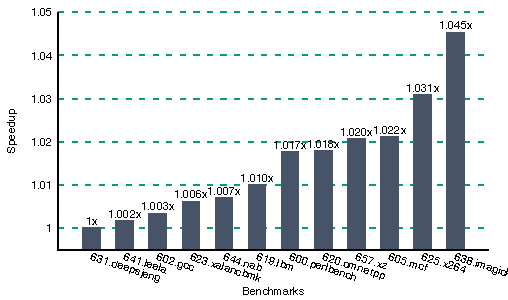
\includegraphics[width=0.45\linewidth]{figures/spec/spec-intel.pdf}
%   }
%   \hfill
%   \subfloat[Compilation time in seconds\label{fig:spec-intel-compilation-time}]{
%     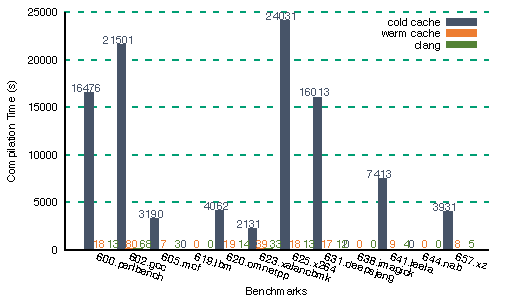
\includegraphics[width=0.45\linewidth]{figures/spec/spec-intel-compiletime.pdf}
%   }
%   \caption*{Targeting Intel Cascade Lake\label{fig:spec-intel}}
%   \hfill
%   \subfloat[Normalized speedup; geomean = 1.012x\label{fig:spec-amd-speed-ups}]{
%     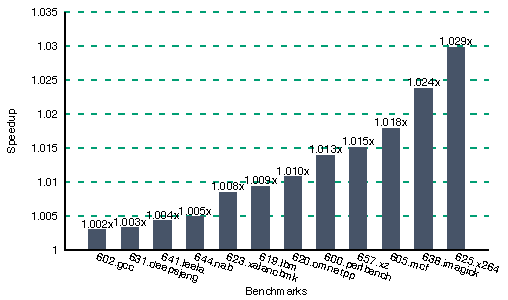
\includegraphics[width=0.45\linewidth]{figures/spec/spec-amd.pdf}
%   }
%   \hfill
%   \subfloat[Compilation time in seconds\label{fig:spec-amd-compilation-time}]{
%     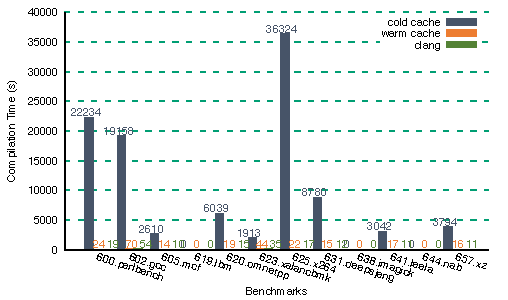
\includegraphics[width=0.45\linewidth]{figures/spec/spec-amd-compiletime.pdf}
%   }
%   \caption*{Targeting AMD Zen 3\label{fig:spec-amd}}
%   \caption{SPEC CPU2017 benchmark performance and compilation time}
%   \label{fig:spec}
% \end{figure*}

\begin{figure}[tbp]
  \centering
  \subfloat[Speedups on Cascade Lake; geomean = 1.015x\label{fig:spec-intel-speed-ups}]{
    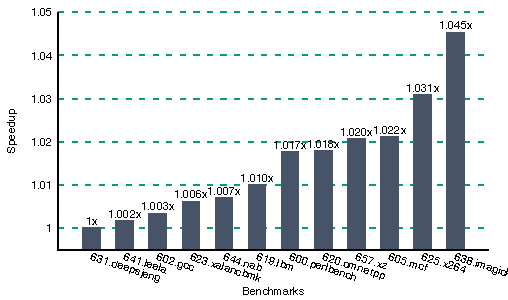
\includegraphics[width=0.48\linewidth]{figures/spec/spec-intel.pdf}
  }
  \hfill
  \subfloat[Speedups on Zen 3; geomean = 1.012x\label{fig:spec-amd-speed-ups}]{
    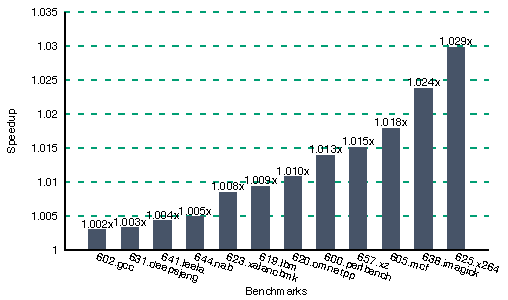
\includegraphics[width=0.48\linewidth]{figures/spec/spec-amd.pdf}
  }
  \caption{SPEC CPU2017 benchmark performance}
  \label{fig:spec}
\end{figure}

\paragraph{Optimizing SPEC CPU2017 with \minotaur{}}

Figure~\ref{fig:spec} shows the effect of optimizing the benchmarks
from SPEC CPU2017 using \minotaur.
%
When optimizing for, and running on, the Intel processor, we observed
a mean speedup of 1.5\%.
%
When optimizing for, and running on, the AMD processor, we observed a
mean speedup of 1.2\%.
%
It is notoriously difficult to speed up the SPEC CPU benchmarks
because compiler engineers have already put considerable effort into
achieving good code generation for them.



\subsection{Optimizations Discovered by \minotaur}
\label{sec:examples}

The purpose of this section is to examine \minotaur's strengths by
presenting some optimizations that it found while compiling benchmark
programs.
%
None of these optimizations can be performed by the version of LLVM
that \minotaur{} is based on,
%\footnote{\minotaur{} uses LLVM~18.1.0 for all results in this paper.}
at its \texttt{-O3} optimization level.
%
We present optimizations in an SSA format that is close to LLVM IR,
but we have edited it slightly for compactness and legibility.

\iffalse
One might be inclined to ask, while reading this section, ``Why is
LLVM incapable of performing this transformation?''
%
Alas, there is no single answer.
%
In some cases, performing the transformation would require the
optimizer to have a semantic model of a processor-specific intrinsic
function, but mostly these models do not exist.
%
In other cases, such as Example~5 below, generic reasoning about the
code would be very difficult, and a specific pattern matcher might not
be robust enough to be worth implementing.
%
Finally, our observation is that vector support in LLVM is somewhat
newer and less mature than support for other IR features, and the
optimizers have simply not had enough time to accumulate the requisite
optimizations.
\fi


\paragraph*{Example 1}

This code is from perlbench in SPEC:

{\small\begin{quote}\begin{verbatim}
%0 = zext <16 x i8> %x to <16 x i16>
%1 = zext <16 x i8> %y to <16 x i16>
%2 = call @llvm.x86.avx2.pavg.w(%0, %1)
%3 = trunc <16 x i16> %2 to <16 x i8>
ret <16 x i8> %3
  =>
%0 = call @llvm.x86.sse2.pavg.b(%x, %y)
ret <16 x i8> %0
\end{verbatim}
\end{quote}}

The unoptimized code zero-extends each 8-bit element of the two input
vectors to 16~bits, calls the AVX2 variant of \texttt{pavg} to perform
element-wise averaging of the extended vectors, and then truncates
elements of the resulting vector back to eight bits.
%
The optimized code simply calls an SSE2 version of the \texttt{pavg}
instruction that operates on 8-bit elements, reducing the uOp cost
of the operation from four to one.


\paragraph*{Example 2}
%https://godbolt.org/z/vjjr7MGzb

This code is from libYUV, ``... an open source project that includes
YUV scaling and conversion
functionality'':
%m\footnote{\url{https://chromium.googlesource.com/libyuv/libyuv/}}

{\small\begin{quote}\begin{verbatim}
%0 = call @llvm.x86.avx2.pmadd.wd(%x, <0,1,0,1, ...>)
%1 = call @llvm.x86.avx2.pmadd.wd(%x, <1,0,1,0, ...>)
%2 = sub nsw <8 x i32> %1, %0
ret <8 x i32> %2
  =>
%0 = call @llvm.x86.avx2.pmadd.wd(%x,<1,-1,1,-1, ...>)
ret <8 x i32> %0
\end{verbatim}
\end{quote}}

The \texttt{pmadd.wd} (multiply and add packed integers) instruction multiplies
signed 16-bit integers element-wise from two input vectors, and then
computes its output by adding adjacent pairs of elements from the
resulting vector.
%
Thus, the input to this instruction is two 16-way vectors containing
16-bit elements, and its output is a single 8-way vector of 32-bit
elements.


In this example, the second argument to each \texttt{pmadd.wd}
instruction in the unoptimized code is a vector of alternating zeroes
and ones, which has the effect of selecting odd-indexed elements into
\texttt{\%0} and even-indexed elements into \texttt{\%1}.
%
Then, after the \texttt{sub} instruction, which simply performs
element-wise subtraction of \texttt{\%0} and \texttt{\%1}, the overall
effect of this code is to compute the difference between adjacent
pairs of elements of \texttt{\%x}.
%
\minotaur{} is able to perform this same computation using a single
\texttt{pmadd.wd} instruction which negates odd-numbered elements of
\texttt{\%x} before performing the addition.
%
The optimized code requires $5$ uOps to execute whereas the original
code requires $8$.


\paragraph*{Example 3}

This code is from libYUV:

%https://godbolt.org/z/7ooobqofK
{\small\begin{quote}\begin{verbatim}
%0 = shufflevector <32 x i8> %x, poison, <3, 7, 11, 15, 19, 23, 27, 31>
%1 = lshr %0, <6, 6, 6, 6, 6, 6, 6, 6>
%2 = zext 8 x i8> %1 to <8 x i32>
ret <8 x i32> %2
  =>
%0 = bitcast <32 x i8> %x to <8 x i32>
%1 = call @llvm.x86.avx2.psrli.d(<8 x i32> %0, 30)
ret <8 x i32> %1
\end{verbatim}
\end{quote}}

The \texttt{shufflevector} instruction in the unoptimized code selects
every fourth byte-sized element from the input \texttt{\%x}.
%
The resulting 8-way vector is right-shifted element-wise by six bit
positions, and that result is zero-extended to an 8-way vector of
32-bit elements.
%
\minotaur's optimized version (which executes in 4 uOps instead of 11)
first reinterprets the input vector's data as 32-bit elements; this
bitcast is relevant to LLVM's type system, but it is a nop at the CPU
level.
%
Then, the \texttt{prsli} instruction shifts each 32-bit element to the
right by 30 bit positions.
%
This right-shift-by-30 achieves the same effect as the unoptimized
code, where the \texttt{shufflevector} can be seen as a
right-shift-by-24, followed by an explicit right-shift-by-6.

\paragraph*{Example 4}

This code, from compiling perlbench from SPEC CPU 2017, illustrates
\minotaur's ability to reason about control flow:

% control flow divergence
%https://godbolt.org/z/e8jTsTMMz
{\small\begin{quote}\begin{verbatim}
entry:
  br i1 %c, label %body, label %if.end
body:
  br label %if.end
if.end:
  %p1 = phi [ %a, %body ], [ %b, %entry ]
  %p2 = phi [ %b, %body ], [ %a, %entry ]
  %r = call @llvm.x86.avx2.pavg.b(%p1, %p2)
  ret <32 x i8> %r
    =>
  %r = call @llvm.x86.avx2.pavg.b(%a, %b)
  ret <32 x i8> %r
\end{verbatim}
\end{quote}}

The intent of the code is to compute the element-wise average of input
vectors \texttt{\%a} and \texttt{\%b}, with a Boolean value
\texttt{\%c} determining the order in which the input vectors are
presented to the \texttt{pavg} instruction.
%
However, the order of arguments to this instruction does not matter, and
\minotaur's version executes in 4 uOps while the original code requires
10.
%
Note that \minotaur{} was not explicitly taught that \texttt{pavg} is
commutative; the necessary information was inferred naturally from the
formal specification.


\paragraph*{Example 5}

This is an optimization discovered
by \minotaur{} when it was used to compile GMP, the GNU Multiple Precision
Arithmetic Library, a widely-used library for arbitrary precision
integer computation:
%q\footnote{\url{https://gmplib.org/}}

% before 19 after 13

{\small\begin{quote}\begin{verbatim}
%0 = lshr i64 %x, 1
%1 = and i64 %0, 0x5555555555555555
%2 = sub i64 %x, %1
%3 = lshr i64 %2, 2
%4 = and i64 %2, 0x3333333333333333
%5 = and i64 %3, 0x3333333333333333
%6 = add nuw nsw i64 %4, %3
%7 = lshr i64 %6, 4
%8 = add nuw nsw i64 %7, %6
%9 = and i64 %8, 0xf0f0f0f0f0f0f0f
ret i64 %9
  =>
%0 = bitcast i64 %x to <8 x i8>
%1 = call @llvm.ctpop(<8 x i8> %0)
%2 = bitcast <8 x i8> %1 to i64
ret i64 %2
\end{verbatim}
\end{quote}}

%
% \vspace{0.1in}
% %
% \caption{On the left, LLVM IR extracted from GMP; when compiled to
%   x86-64 code and run on an Intel Cascade Lake processor, its
%   predicted execution cost is 19 uOps. On the right, \minotaur's
%   optimized version of this code, which requires 13 uOps on the same
%   target.}
% \label{fig:ctpop}
% \end{figure*}
%
The original code performs a series of bit-level
manipulations on a 64-bit integer value, with the net result of
performing an 8-way vectorized 8-bit popcount operation.\footnote{The
popcount, or Hamming weight, of a bitvector is the number of ``1''
bits in it.}
%
The optimized code simply calls an intrinsic function to do the
popcount; it costs 13 uOps instead of the original code's 19.
%
Although robust recognition of open-coded idioms is not the focus
of our work, \minotaur{} does sometimes manage to achieve this.

Taking a strict view of types in the synthesis process could help
prune the search space, but it would also cause us to miss
optimizations that require a flexible view of types.
%
This example illustrates the latter case: the original code contains
no indication that a good optimization can be found using a vector of
type <8 x i8>, and therefore a strictly type-guided synthesis
procedure would miss this one.

\paragraph*{Example 6}

This code comes from 644.nab in SPEC CPU 2017:

% https://github.com/llvm/llvm-project/issues/85250
{\small\begin{quote}\begin{verbatim}
%0 = fcmp oge float %x, 0.000000e+00
%1 = fneg float %x
%2 = select i1 %0, float %0, float %2
%3 = fcmp oeq float %2, 0.000000e+00
ret i1 %3
  =>
%1 = fcmp oeq float %x, 0.000000e+00
ret i1 %oeq
\end{verbatim}
\end{quote}}

The original code computes the absolute value of a floating-point
number \texttt{\%x} and then checks if the result is zero.
\minotaur{} found that that the original code is equivalent to simply checking if
\texttt{\%x} is zero.


\paragraph*{Example 7}

This code is from the SPEC CPU 2017 benchmark 619.lbm:

% https://github.com/llvm/llvm-project/issues/85245
{\small\begin{quote}\begin{verbatim}
%0 = fsub float %x, %y
%1 = fcmp ogt float %0, 0.000000e+00
ret i1 %3
  =>
%0 = fcmp ogt float %x, %y
ret i1 %0
\end{verbatim}
\end{quote}}

The original code computes the difference between two floating-point
values, and then checks if the result is greater than zero. \minotaur{}
found that this code is equivalent to checking if the second value is
less than the first.


\paragraph*{Example 8}

This code comes from 619.lbm in SPEC CPU 2017:

% https://github.com/llvm/llvm-project/issues/85267

{\small\begin{quote}\begin{verbatim}
%0 = fmul float %x, 0x3FF0CCCCC0000000
%1 = fcmp olt float %t1, 0x3FE20418A0000000
ret i1 %1
  =>
%0 = fcmp ole float %x, 0x3FE12878E0000000
ret i1 %0
\end{verbatim}
\end{quote}}

The original code multiplies a floating-point value \texttt{\%x} by a
constant, and then checks if the result is less than another constant.
\minotaur{} found that this code is equivalent to checking if \texttt{\%x}
is less than or equal to a third constant.
It is tricky to reason about floating-point literals, and \minotaur{} is able to
reason and synthesize the correct literals correctly.

\paragraph*{Example 9}

This code comes from 638.imagick in SPEC CPU 2017:

{\small\begin{quote}\begin{verbatim}
%0 = fmul float %x, 0.000000e+00
%1 = fmul float %0, 3.000000e+00
ret float %1
  =>
%0 = fmul float %x, 0.000000e+00
ret i1 %0
\end{verbatim}
\end{quote}}

The original code multiplies a floating-point value \texttt{\%x} by
zero, and then multiplies the result by 3.0. \minotaur{} found that this
code is equivalent to multiplying \texttt{\%x} by zero directly.
Note the original code cannot be optimized to 0.0 directly, because of
the NaN and signed zero propagation rules in floating-point arithmetic.
This example shows that \minotaur{} is able to reason about these corner
cases and synthesize the correct code.

% \paragraph*{Example 10}


%TODO: Add one final example
% place holder for a good example





\section{Related Work}

A \emph{superoptimizer} is a program optimizer that meaningfully
relies on search to generate better code, in contrast with traditional
compilers that attempt a fixed (but perhaps very large) sequence of
transformations.
%
The eponymous superoptimizer~\cite{massalin} exhaustively generated
machine instruction sequences, using various strategies to prune the
search space, and using testing to weed out infeasible candidates.
%
Also predating modern solver-based methods, Davidson and Fraser~\cite{peep84}
constructed peephole optimizations from machine description files.
%
In contrast, modern superoptimizers rely on solvers to perform
automated reasoning about program semantics.


Souper~\cite{souper} is a synthesizing superoptimizer that works on
LLVM IR; it is the most directly connected previous work to \minotaur{}.
%
Souper's slicing strategy is similar to \minotaur's in that it extracts a
DAG of LLVM instructions that overapproximates how a given SSA value
is computed.
%
However, unlike Souper, \minotaur{} extracts memory operations and
multiple basic blocks, so it is capable of (we believe) strictly more
transformations than Souper is able to perform.
%
Additionally, Souper's undefined behavior model does not capture all
of the subtleties of undefined behavior in LLVM, whereas we reuse
Alive2's model, which is probably the most widely used formalization
of these semantics, and is generally recognized as being correct.
%
Finally, \minotaur{} focuses on vector-related transformations, whereas
Souper supports neither LLVM's portable vector instruction set nor its
platform-specific intrinsics.


\minotaur{} is also strongly inspired by Bansal and Aiken's
work~\cite{Bansal06}; their superoptimizer operated on x86 assembly
code and was able to make interesting use of vector instructions.
%
Starting from unoptimized assembly produced by GCC, it was able to
produce code competitive with higher optimization levels.
%
The overall structure of this superoptimizer, where program slices
are extracted, canonicalized, checked against a cache, and then
optimized in the case of a cache miss, is very similar to \minotaur{}, but
there are many differences in the details, particularly in \minotaur's
slice extractor which allows its synthesis specification to
approximate the original code's effect much more closely.
%
Another assembly superoptimizer, STOKE~\cite{stoke,stoke-fp,conditionally},
is not as closely related; it is based on randomly
perturbing assembly-language functions.
%
STOKE can potentially perform transformations that Minotaur cannot,
but we believe that its results are more difficult to translate into
standard peephole optimizations than are Minotaur's.


Several recent projects have focused not on optimizing individual
programs but rather on generating program rewrite rules.
%
OptGen~\cite{optgen} finds scalar peephole optimizations that meet
a specified syntactic form.
%
Even at small rewrite sizes, it was able to find numerous
optimizations that were missing from the 2015 versions of GCC and
LLVM\@.
%
VeGen~\cite{vegen} generates SLP vectorization rules---an SLP
vectorizer~\cite{slp} merges a set of scalar operations into vector
instructions.
%
VeGen parses the Intel Intrinsics Guide~\cite{intelguide} and uses this
to build pattern matchers for x86 vector instructions.
%
VeGen applies the pattern matchers to an input scalar program, and
replaces scalar expressions with vector instructions when it
finds a profitable match.
%
VeGen uses syntactic pattern matching rather than solver-based
equivalence/refinement checking.
%
Diospyros~\cite{diospyros} is another vector rewrite rule generator,
it takes an equality saturation~\cite{equalitysat} approach and uses a translation
validator to reject unsuitable candidates.
As an equality saturation-based tool, Diospyros builds its search space
with existing rewrite rules.


Program synthesis---generating implementations that conform to
a given specification---is intimately related to superoptimization.
%
Rake~\cite{rake} performs instruction selection for vectorized
Halide~\cite{halide} expressions using a two stage synthesis
algorithm.
%
First, Rake synthesizes a data-movement-free sketch~\cite{sketch}, and
then in the second stage it concretizes data movement for the
sketch via another synthesis query.
%
Rake targets Hexagon DSP processors~\cite{hexagon} which share some functionally
similar SIMD instructions with x86\@.
%
Cowan et al.~\cite{ml_syn} synthesized quantized machine learning
kernels.
%
Their work introduces two sketches: a compute sketch, which computes a matrix
multiplication, and a reduction sketch that collects the computation
result to the correct registers.
%
It relies on Rosette~\cite{rosette} to generate an efficient NEON~\cite{neon}
implementation that satisfies the specifications for those two
sketches.
%
Swizzle Inventor~\cite{swizzleinventor} is another tool built on
Rosette; it synthesizes data movement instructions for a GPU compute
kernel, and it requires user-defined sketches describing the
non-swizzle part of the program.
%
MACVETH~\cite{sparse} generates high-performance vector packings of
regular strided-access loops, by searching for a SIMD expression that
is equivalent to a gather specification.
%
All of these works show good performance results, but they focus on
relatively narrow tasks, whereas \minotaur{} attempts to improve SIMD
programs in general.


Most previous superoptimizers and program synthesizers use simple
cost models.
%
For example, Souper~\cite{souper} assigns each kind of instruction a
weight and uses the weighted sum as the cost of a rewrite.
%
This kind of cost model is not a very good predictor of performance
on a modern out-of-order processor.
%
\minotaur{} and MACVETH~\cite{sparse} use the LLVM-MCA~\cite{llvmmca}
microarchitectural performance analyzer, which can still lead to
mispredictions, but it is generally more accurate than simple
approaches are.

\section{Conclusion}
\label{sec:conc}

We created \minotaur{} because we noticed that LLVM appeared to be missing
relatively obvious optimizations in code containing both its portable
vector instructions and also its platform-specific intrinsic
functions that provide direct access to hardware-level primitives.
%
\minotaur{} cuts loop-free DAGs of instructions---including branches and
memory operations---out of LLVM functions and then attempts to
synthesize better implementations for them.
%
When improved code is found, the optimization is performed and also
the synthesis result is cached.
%
On the libYUV test suite, \minotaur{} gives speedups up to 1.64x,
with an average speedup of 2.2\%.
%
We expect to see impact not by convincing application developers to
use \minotaur, but rather by convincing compiler developers to implement
useful optimizations that we can discover.




\iffalse
\paragraph{Who is supposed to use \minotaur{}, and how?}
%
Even with a warm cache, \minotaur{} is almost certainly too slow for
developers to use during their day-to-day life.
%
It could instead be used to build final software releases, which are
infrequent enough that long compile times might not be a big problem.
%
However, our guess is that the most likely users for \minotaur{} are
compiler developers, who would use it to discover optimizations and
then cherry-pick the best of these and add them, by hand, to the LLVM
implementation.


\paragraph{Why does \minotaur{} sometimes make code run slower?}
%
There are three main reasons why our
superoptimizer sometimes performs transformations that make code
slower.
%
First, its cost model takes a myopic view of the code being compiled,
looking only at the (predicted) performance of an extracted cut.
%
It could be the case that a locally profitable transformation is
unprofitable in a larger context, for example because the optimized
code relies on a processor port that is already highly contended.
%
Second, \minotaur{} runs in the middle of a long sequence of LLVM
transformation passes, and we do not attempt to model or predict how it
might interact with them.
%
It seems probable that our tool sometimes makes changes that interfere
with LLVM transformations downstream in the pass pipeline.
%
For example, even small changes to the size of functions can cause the
backend to make different decisions, which can lead to performance effects.
%
Third, we fundamentally rely on LLVM-MCA to accurately assess the cost
of running a cut on the target microarchitecture.
%
However, LLVM-MCA is known to contain inaccuracies~\cite{ithemal}.


\paragraph{Future work}
%
Several enhancements and future projects suggest themselves:
%
\begin{itemize}
\item
We would love to synthesize floating point optimizations, but our
experiments in that direction have so far not been promising; the
solver is the bottleneck.
\item
In addition to a middle-end superoptimizer like \minotaur{}, LLVM should
have a backend superoptimizer that runs on, for example, its MIR
(machine intermediate representation).
\item
Instead of synthesizing $1$--$3$ instructions per optimization, we would
like to be synthesizing $5$--$10$ of them.
%
A tool that could do this would seem to be qualitatively more powerful
than a standard peephole optimizer.
%
However, the size of the search space is daunting.
\end{itemize}
%
Generating compiler optimizations by looking into large search spaces
has been a dream for more than 40 years, we look forward to pushing
this idea a little farther.
\fi


\chapter{Synthesizing Optimal Collective Algorithms}
\label{chap:sccl}
\newcommand{\CC}{C\nolinebreak\hspace{-.05em}\raisebox{.4ex}{\tiny\bf +}\nolinebreak\hspace{-.10em}\raisebox{.4ex}{\tiny\bf +}}
\def\CC{{C\nolinebreak[4]\hspace{-.05em}\raisebox{.4ex}{\tiny\bf ++}}}

\newcommand{\gathercoll}{Gather\xspace}
\newcommand{\allgather}{Allgather\xspace}
\newcommand{\scatter}{Scatter\xspace}
\newcommand{\reduce}{Reduce\xspace}
\newcommand{\broadcast}{Broadcast\xspace}
\newcommand{\reducescatter}{Reducescatter\xspace}
\newcommand{\allreduce}{Allreduce\xspace}
\newcommand{\alltoall}{Alltoall\xspace}

\newcommand{\dgxone}{DGX-1\xspace}
\newcommand{\dgxtwo}{DGX-2\xspace}
\newcommand{\amd}{AMD\xspace}

\newcommand{\chunkstep}[2]{$#1$-chunk $#2$-step\xspace}


\newcommand{\tool}{SCCL}
\newcommand{\toollong}{Synthesized Collective Communication Library}

\newcommand{\setwhere}{\;|\;} % the bar in middle of set builder notation
\newcommand{\qst}{\;} % the "such that" symbol for quantifiers. Could also be . or :
\newcommand{\powerset}{\mathcal{P}}
\newcommand{\posint}{\mathbb{Z}_{\geq0}}
\newcommand{\oftype}{\mathbin{:}}
\newcommand{\range}[1]{\left[#1\right]}
\newcommand{\dotscend}{\dotsc\hspace{-0.08em}}

\newcommand{\Ite}[3]{\mathrm{ITE}(#1,#2,#3)}
% \newcommand{\Ite}[3]{\text{if }#1\text{ then }#2\text{ else }#3}

% Synthesis stuff
\newcommand{\collectiveproblem}{\textsc{SynColl}\xspace}
\newcommand{\bcastproblem}{\textsc{SynCollBcast}\xspace}
\newcommand{\reducingproblem}{\textsc{SynCollReduce}\xspace}
\newcommand{\size}{P}
\newcommand{\ids}{I}
\newcommand{\pre}{\mathit{pre}}
\newcommand{\post}{\mathit{post}}
\newcommand{\chunk}{C}
\newcommand{\gchunk}{G}
\newcommand{\toglobal}{\mathit{ToGlobal}}
\newcommand{\steps}{S}
\newcommand{\rounds}{R}
\newcommand{\fb}{k}
\newcommand{\bw}{B}
\newcommand{\rparts}{Q}
\newcommand{\sends}{T}
\newcommand{\start}[2]{\mathit{time}_{#1,#2}}
\newcommand{\send}[3]{\mathit{snd}_{#1,#2,#3}}
\newcommand{\qouta}{\mathit{Q}}

\newcommand{\broadcasting}{non-com\-bin\-ing\xspace}
\newcommand{\broadcastingCap}{Non-com\-bin\-ing\xspace}
\newcommand{\reducing}{com\-bin\-ing\xspace}
\newcommand{\reducingCap}{Com\-bin\-ing\xspace}

\newcommand{\etal}{\textit{et al}.}

This chapter is adapted from PPoPP'21 paper ``Synthesizing Optimal
Collective Algorithms'' authored by myself, Zixian Cai, Saeed Maleki,
Madan Musuvathi, Todd Mytkowicz, Jacob Nelson and Olli Saarikivi.
Zixian Cai and me are the co-first authors of the paper.

\newcommand{\CC}{C\nolinebreak\hspace{-.05em}\raisebox{.4ex}{\tiny\bf +}\nolinebreak\hspace{-.10em}\raisebox{.4ex}{\tiny\bf +}}
\def\CC{{C\nolinebreak[4]\hspace{-.05em}\raisebox{.4ex}{\tiny\bf ++}}}

\newcommand{\gathercoll}{Gather\xspace}
\newcommand{\allgather}{Allgather\xspace}
\newcommand{\scatter}{Scatter\xspace}
\newcommand{\reduce}{Reduce\xspace}
\newcommand{\broadcast}{Broadcast\xspace}
\newcommand{\reducescatter}{Reducescatter\xspace}
\newcommand{\allreduce}{Allreduce\xspace}
\newcommand{\alltoall}{Alltoall\xspace}

\newcommand{\dgxone}{DGX-1\xspace}
\newcommand{\dgxtwo}{DGX-2\xspace}
\newcommand{\amd}{AMD\xspace}

\newcommand{\chunkstep}[2]{$#1$-chunk $#2$-step\xspace}


\newcommand{\tool}{SCCL}
\newcommand{\toollong}{Synthesized Collective Communication Library}

\newcommand{\setwhere}{\;|\;} % the bar in middle of set builder notation
\newcommand{\qst}{\;} % the "such that" symbol for quantifiers. Could also be . or :
\newcommand{\powerset}{\mathcal{P}}
\newcommand{\posint}{\mathbb{Z}_{\geq0}}
\newcommand{\oftype}{\mathbin{:}}
\newcommand{\range}[1]{\left[#1\right]}
\newcommand{\dotscend}{\dotsc\hspace{-0.08em}}

\newcommand{\Ite}[3]{\mathrm{ITE}(#1,#2,#3)}
% \newcommand{\Ite}[3]{\text{if }#1\text{ then }#2\text{ else }#3}

% Synthesis stuff
\newcommand{\collectiveproblem}{\textsc{SynColl}\xspace}
\newcommand{\bcastproblem}{\textsc{SynCollBcast}\xspace}
\newcommand{\reducingproblem}{\textsc{SynCollReduce}\xspace}
\newcommand{\size}{P}
\newcommand{\ids}{I}
\newcommand{\pre}{\mathit{pre}}
\newcommand{\post}{\mathit{post}}
\newcommand{\chunk}{C}
\newcommand{\gchunk}{G}
\newcommand{\toglobal}{\mathit{ToGlobal}}
\newcommand{\steps}{S}
\newcommand{\rounds}{R}
\newcommand{\fb}{k}
\newcommand{\bw}{B}
\newcommand{\rparts}{Q}
\newcommand{\sends}{T}
\newcommand{\start}[2]{\mathit{time}_{#1,#2}}
\newcommand{\send}[3]{\mathit{snd}_{#1,#2,#3}}
\newcommand{\qouta}{\mathit{Q}}

\newcommand{\broadcasting}{non-com\-bin\-ing\xspace}
\newcommand{\broadcastingCap}{Non-com\-bin\-ing\xspace}
\newcommand{\reducing}{com\-bin\-ing\xspace}
\newcommand{\reducingCap}{Com\-bin\-ing\xspace}

\newcommand{\etal}{\textit{et al}.}

\section{Introduction}
% Machine learning workloads imply novel topologies
Recent trends in machine learning towards training and serving large models together with the stagnation of Moore's-law-induced compute performance has led system designers to include novel high-bandwidth interconnect networks both within and across nodes in distributed clusters. For instance, a \dgxone server consists of two x86 processors and eight GPUs, interconnected by NVIDIA's NVLink network as shown in Figure~\ref{fig:dgx1-topo}. These networks' designs are motivated as much by the need to perform efficient \allreduce, a crucial primitive in machine learning, as well as by hardware considerations such as signal integrity, cooling and physical layout.
%\todo{only NVLink is shown in the figure, maybe reword the sentence or change the figure?
%Actually, I am not even sure if a socket contains THOSE four GPUs.}
A wide variety of similar accelerators with novel high-speed interconnects are used to train machine learning models today, including AMD's MI50 GPUs~\cite{mi50}, Graphcore's IPUs~\cite{graphcore} and Google's TPUs~\cite{tpu}.
%\todo{We mention distributed clusters but don't otherwise address them in the paper, I think}

% Hand-written communication primitives - what are the problems.
These novel topologies require novel communication kernels to maximize performance. Today these kernels are written and optimized manually. For instance, NVIDIA Collective Communication Library (NCCL) has two general algorithms for the supported operations such as \allreduce: a high-bandwidth ring algorithm and a low-latency tree algorithm. These implementations are manually written and they do not necessarily have the best performance for different topologies including \dgxone's. On one hand, repeating this manual effort for other communication primitives such as \alltoall or extending already implemented algorithms to a wide variety of hardware topologies is simply infeasible.
%\todo{maybe just say communication algorithms, as ring/tree algorithms are mentioned later}

On the other hand, optimizing these communication kernels for performance for each topology and buffer size is crucial. For instance, we found 30\% of the training time for the 8.3 billion parameter Megatron language model with model parallelism is spent inside \allreduce where each
buffer is of medium size (10-100MB). Also, for data parallelism, the communication buffers
could range from a few KBs (one layer) to a few GBs (the entire model).
We expect this wide range of sizes as large models are developed and trained on
larger distributed clusters.

%As machine learning models growing both in size and training complexity, the
%potential payoffs for such automation are significant in our current world. For
%example, when the 8.3 billion parameter Megatron language model is trained with
%8-way model parallelism on an NVIDIA DGX-1~\cite{megatronlm-arxiv}, 30\% of the
%training time is spent on communication.

%GPUs are used to accelerate a wide variety of tasks, from machine learning to
%simulations for engineering and physics. As the complexity of these tasks grows,
%there is a trend to pack an increasing number of GPUs inside a single node. This
%in turn places increasing importance on the mechanisms for GPU-to-GPU
%communication.

%In contrast with traditional inter-node networks, the interconnects for GPUs
%inside a node are often highly asymmetric. This is caused by a number of
%concerns, such as limitations on wire length and signal quality requirements for
%high-bandwidth links such as PCIe and NVLink as well as limitations on GPU
%placement due to cooling and physical layout. This results in in-node networks
%often not corresponding to any widely studied network topology (e.g., butterfly
%or hypercube). \todo{Give an example here?}

%Just like in traditional networks, the communication patterns have to be
%tailored to the topology for maximum performance. This has been done in isolated
%cases as, for example, NVIDIA Collective Communication Library (NCCL) implements
%algorithms optimized for their 8 GPU DGX-1 servers (see Figure~\ref{fig:dgx1-topo}). However, the wide variety of
%available hardware targets means that it is hard for a library to provide
%optimal algorithms for all configurations, which makes this an ideal target for
%automation.

\begin{figure}[tbp]
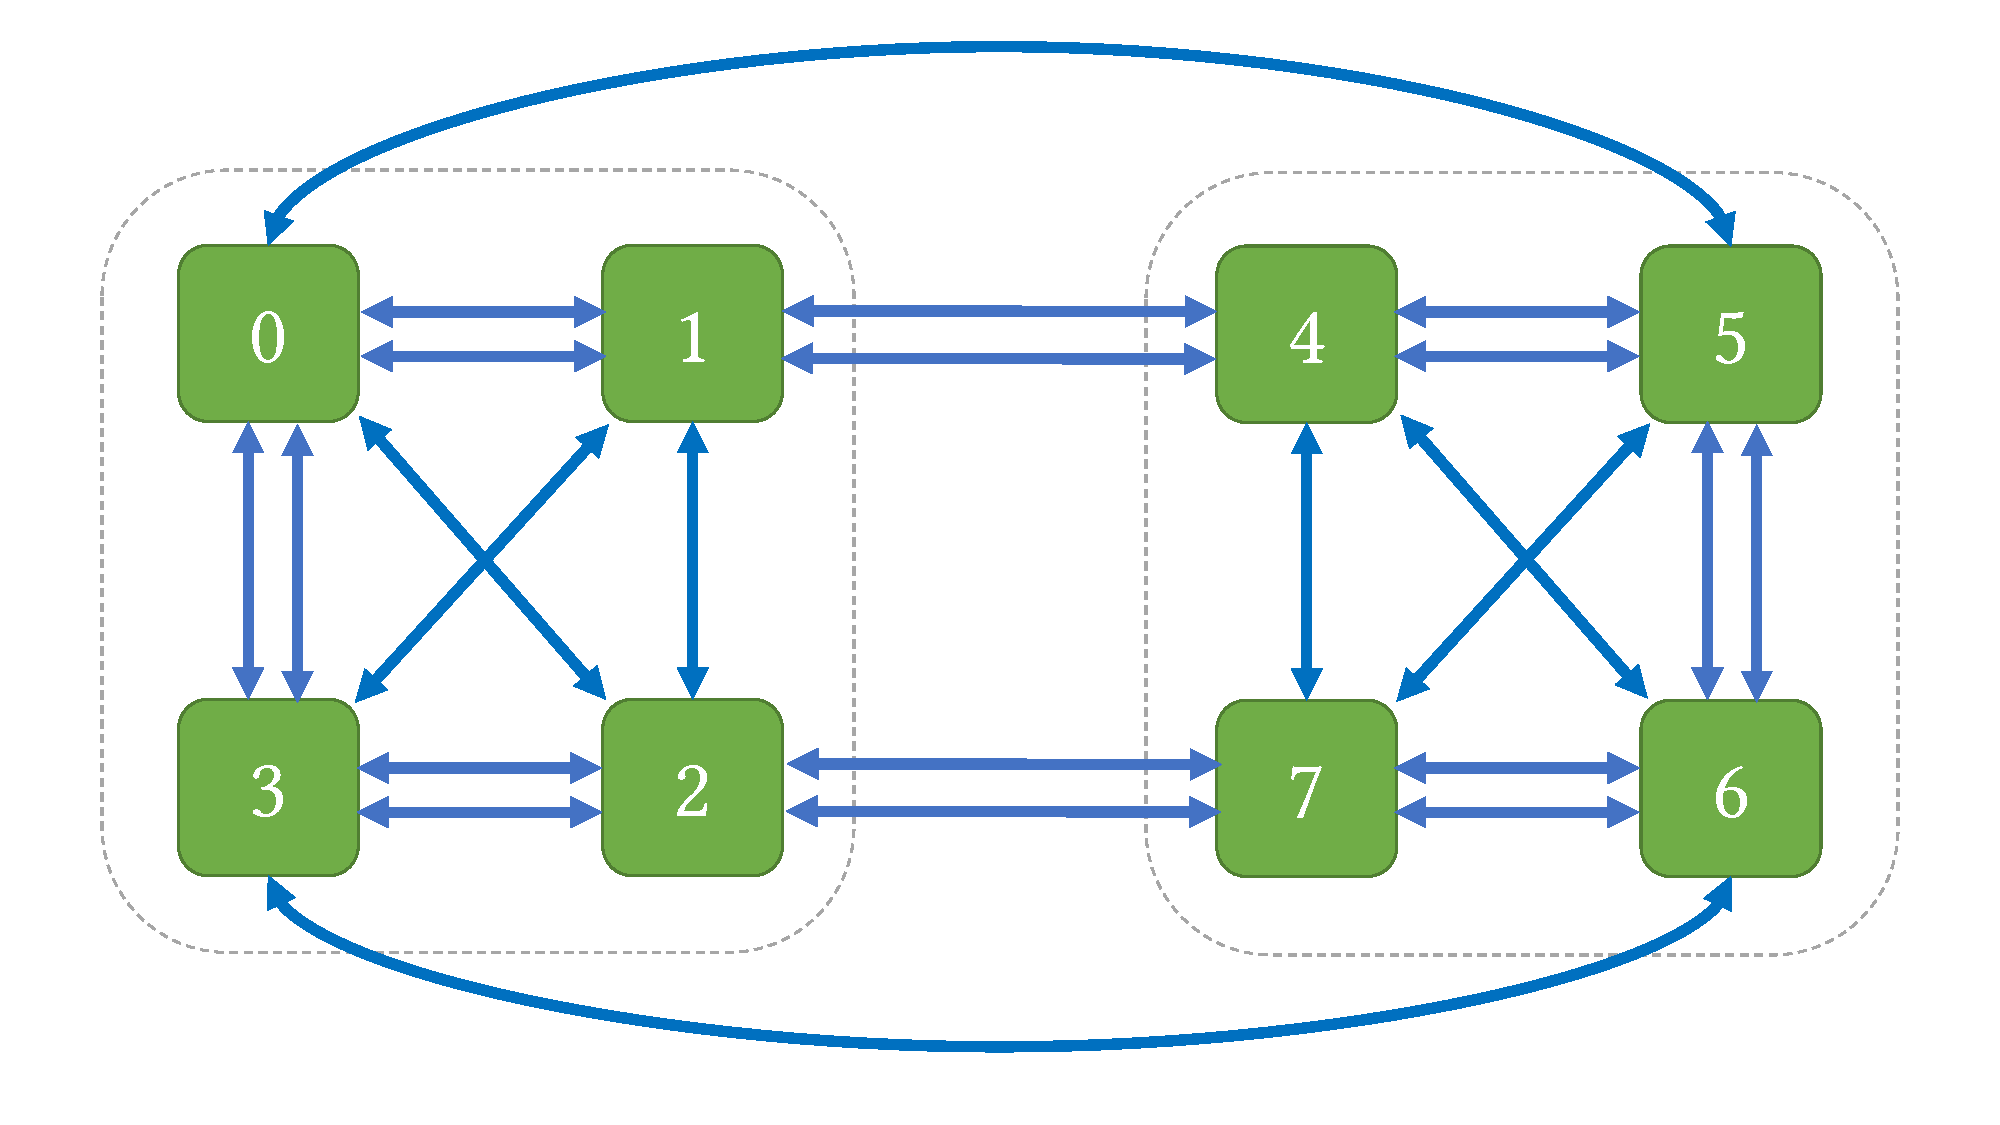
\includegraphics[page=1,width=\columnwidth]{figures/topos.pdf}
\caption{NVLink topology of an NVIDIA DGX-1.}
\label{fig:dgx1-topo}
\end{figure}
%\todo{the grey box indicating a socket has a low contrast when printed. colours for two different rings should have higher contrast (blue and orange perhaps?)}

% explain our approach
In this chapter, we automatically synthesize high-performance communication kernels.
Given a topology, specified as a graph with bandwidth constraints on nodes and edges, and a communication primitive, specified as the pre- and post-condition on data location and computation on it, we generate~(Section~\ref{sec:synthesis}) a quantifier-free SMT formula that captures the set of all feasible algorithms that implement the primitive on the input topology.
Exploring this space to appropriately minimize the number of communication steps or decrease the granularity of communication at each step, is a computationally difficult problem. We exploit
an SMT solver to synthesize algorithms that explore this tradeoff along the Pareto frontier between latency-optimality and bandwidth-optimality.
For every solution from the SMT solver, we automatically generate and lower~(Section~\ref{sec:lowering}) high-performance implementations.


% We approach this problem as a synthesis problem. Collective communication
% primitives can be specified in terms of pre- and post-conditions on which
% processes data resides on and optionally where a user specified reduction
% function has been applied. We encode pre- and post-conditions as well as actions
% to move data between processes as quantifier-free SMT formulas, which we solve
% using Z3. We further impose constraints on bandwidth usage based on the topology
% of the specific machine we are targeting and limit the number of steps for the
% whole algorithm. This gives us a way to explore the entire space of possible
% algorithms for implementing a given primitive on the target hardware.

% how do we make it scalable
When using SMT, finding the right encoding can make all the difference for the
feasibility of an approach. This paper details the important design choices in
our encoding that help it scale to all of our hardware targets. We use the SMT
encoding for \broadcasting collectives, such as \broadcast, while for \reducing
collectives, such as \reduce, we employ a reduction back to the synthesis
problem for \broadcasting collectives.
%A key observation is that topologies have natural symmetries. Our encoding exploits this symmetry to efficiently explore the space of algorithms without sacrificing satisfiability.
This reduction generalizes a well known fact that some \reducing collectives may
be produced by inverting a \broadcasting one, e.g. \reduce by inverting \broadcast.

%This allows us to reuse
%the synthesis of certain primitives such as \allreduce, further improving our
%scalability.
%\todo{"time time-reversed mirror-image", huh? find easier to understand wording.}
%\todo{what do you mean by "modularize"? it's more like we reduce (no pun intended) the problem of reduction to broadcasting, which is the wording used later in bullet points}

% This informed an optimization in
% our encoding, that allows us to make reasoning about which GPUs data has been
% reduced implicit.

%\todo{This is quite vague right now.}

% The ability to control the number of steps an algorithm must execute in gives us
% a novel capability for trading off between latency and bandwidth optimality. By
% synthesizing a range of algorithms at different points in this space we can use
% the best algorithm for any given message size. While MPI implementations and
% NCCL both switch between algorithms based on message size, our synthesis
% approach allows us to do so in a much more fine grained manner. We show that
% this enables our algorithms to provide better performance than NCCL at all
% message sizes. \todo{Update this claim with truth.}

We implement our approach in a tool called \toollong{}~(\tool{}),
which probes the target hardware topology, synthesizes algorithms for
it using Z3~\cite{z3} and finally generates CUDA code that efficiently implements that algorithm.  These algorithms are
synchronous; at every step of the algorithm, one or more of the nodes
send and/or reduce data from others.
%\todo{"CUDA code"=>hardware dependent code? we have AMD GPUs. From saemal: AMD runs CUDA. OpenCL is another possibility but no one really uses it.}

% algorithmic novelty
Some of the algorithms we synthesize are novel, with no known counterparts in
the literature occupying the same latency-bandwidth tradeoff. For example, we
have produced a latency-optimal 2-step (4-step) algorithm for
the \allgather (\allreduce) primitive in the DGX-1 topology (Figure~\ref{fig:dgx1-topo}) and
a bandwidth-optimal 3-step (6-step) algorithm for the \allgather (\allreduce) primitive on the
same topology.  In addition to providing novel
algorithms, our approach informs us when a combination of bandwidth and number
of steps is \emph{not possible}. This makes our synthesis approach a tool for
probing the algorithmic properties that a given topology provides, which is
useful for co-design of hardware interconnects with communication libraries.
%\todo{"occupying the same latency-bandwidth tradeoff": exhibiting? and being different isn't necessarily good, we want more bandwidth with the same latency or lower latency with the same bandwidth.}
%\todo{tell reader that the "number of steps" correlate with latency?}
% results
Our evaluation~(Section~\ref{sec:evaluation}) shows us that this approach scales and beats NCCL in almost all cases.


To summarize, the contributions of this chapter are as follows:
\begin{itemize}
    \item A formalization of the synthesis problem for \broadcasting collectives.
    \item A general strategy for encoding the synthesis problem for
    collective communications algorithms into the quantifier-free linear integer
    arithmetic (QF\_LIA) sub-logic of the SMT-LIB logic.
    \item A reduction from the synthesis problem for \reducing collectives to that for \broadcasting collectives.
    % \item Explanations of some novel algorithms our synthesis has produced.
    \item A description of how \tool{} generates efficient code for the algorithms we synthesize on nodes with NVIDIA or AMD GPUs.
    \item An evaluation of \tool's generated algorithms on common server topologies for deep learning workloads and a comparison against NCCL.
\end{itemize}

%\todo{Paper structure paragraph?}

%%% Local Variables:
%%% mode: latex
%%% TeX-master: "paper"
%%% End:

\section{Overview}
This section provides an overview of synthesizing latency- and bandwidth-optimal algorithms, using \allgather for the
\dgxone topology~(Figure~\ref{fig:dgx1-topo}) as the running example.

\subsection{Collective Communication Primitives}
\label{sec:background-collectives}
Collective communication primitives allow nodes in a networked system to perform operations on shared data. As an example, if each node has some input data, the \allgather primitive transfers these data to all of the nodes.  One way to implement this is for each node to independently send its data to all other nodes. But, an algorithm in which the nodes collectively work together can be more efficient. The efficiency of such algorithms depends on the network topology.

\begin{comment}
    For instance, given a set of nodes each having an array of data, the \allreduce primitive computes the sum (or some specified associative operation) of all these arrays and stores the result in each of these arrays.

Computing the primitives such as \allreduce requires the nodes to communicate. This communication usually happens in smaller chunks of the input array. Given $N$ nodes, say we split the input array into $N$ chunks, where $c_{i,j}$ represents the $i$th chunk at node $j$. One way to compute \allreduce is as follows. First, we compute at node $i$, a partial sum $d_i = \sum_j c_{i,j}$. These reductions can be performed by arranging $N$ nodes in a spanning tree and communicating chunks $c_{i,j}$ along the tree. Note, there are $N$ parallel reductions each possibly using a different spanning tree. This arrangement of reduced data is called the \reducescatter primitive. Once we have the chunks $d_i$, we can perform an \allgather operation by ensuring each node has a copy of $d_i$. In essence, \allgather involves $N$ simultaneous broadcasts of $d_i$ from node $i$. Thus, we have implemented \allreduce by performing an \reducescatter followed by an \allgather.
\todo{I think the ``$N$ parallel reductions each possibly using a different spanning tree'' makes this confusing---is this describing an approach where each node reduces $1/N$ of the chunks?}
\todo{say "compute at node $i$, a partial sum" of chunk $i$.}
\todo{they're are a part of the sum of arrays. they are not really partial sums, in the sense that, e.g., only data from half of the nodes are added.}
\todo{"there are $N$ parallel reductions"=>these $N$ parallel reductions}

Implementing a collective communication primitive depends on the topology. For instance, when executing parallel reductions or broadcasts in the implementation above, the algorithm has to choose different spanning trees to utilize the bandwidth on all links in the topology. Similarly, the algorithm has to choose the ideal chunk size to use for communication. We will demonstrate these choices for the \dgxone topology described below.
\todo{"Implementing" $\ldots$ efficiently}
\todo{"has to chose ": might have to choose}
\end{comment}

\subsection{Topology}
The network topology specifies how the nodes are connected with each other and the latency and bandwidth constraints on the links connecting them. Consider the \dgxone topology shown in Figure~\ref{fig:dgx1-topo}. It consists of $8$ GPUs (or nodes, in the above formalism) split into two groups $\{0,1,2,3\}$ and $\{4,5,6,7\}$. The nodes in each group are fully connected. In addition, there are four inter-group links as shown in the figure. These nodes are connected through
NVLinks, with some nodes connected with two parallel NVLinks as shown in Figure~\ref{fig:dgx1-topo}.

%There are two kinds of links shown in two different colors. The fast links, such as the one connecting nodes $0$ and $1$ have twice the bandwidth as the (relatively) slow links, such as the one connecting nodes $0$ and $2$. The figure represents the fast links with two arrows. Each link is bidirectional allowing concurrent sends and receives at full bandwidth.
%\todo{Remove the colors and the double arrow should make it clear}
%\todo{Also just mention that they are called nv2 and nv1 links}
%\todo{"split into two" groups, each associated with one CPU socket.}
%\todo{"All the nodes within a socket": all the GPUs in the same group}
%\todo{"inter-socket links" sound like QPI: maybe inter-group?}
%\todo{also check the usage in latency-optimal algorithm}
%\todo{I recommend talking about these in terms of groups rather than sockets to avoid the NVLink/PCIe/QPI confusion too -jn}
%\todo{I also recommend not talking about ``fast'' and ``slow'' links, since the diagram shows a fast link as 2 slow links (which is indeed what it is), and we then talk about using 6 logical rings; better to just say 6 links and 6 rings}

The \dgxone's design was heavily influenced by the need to do gradient reduction for machine learning workloads. Specifically, this topology forms two non-overlapping rings: one connecting nodes $\{0,1,4,5,6,7,2,3\}$ with two NVLinks per edge and another connecting $\{0,2,1,3,6,4,7,5\}$ with one NVLink per edge. These rings are bidirectional and thus form $6$ logical single-NVLink rings. The NCCL library implements \allgather by running $6$ simultaneous ring algorithms as we discuss below.

%Given the fast ring has twice the bandwidth and each ring is bidirectional, this allows the implementation to utilize $6$ logical rings with the same bandwidth %to implement collection primitives
%(2 from the slow ring and 4 from the fast ring).

\subsection{Cost Model}
%\todo{I think we need to define bandwidth and latency optimality here. My understanding is that a bandwidth-optimal algorithm is one that sends the minimal amount of data necessary to complete its operation, and a latency-optimal one uses the fewest number of communication rounds possible to complete its operation. Is that what we mean?}

%Before discussing how to build bandwidth- and latency-optimal algorithms for this topology, we will introduce a simple cost model.
We will characterize the communication cost using the $(\alpha, \beta)$ model~\cite{hockney1994communication}. That is, sending a message of size $L$ along a link costs $\alpha + L\cdot\beta$ time.
Here, $\alpha$ is the latency of communication and captures the {\em fixed} costs, such as the overhead of initiating a transfer or invoking a GPU kernel,
and $\beta$ is the inverse bandwidth of the link and captures {\em per-byte} costs, such as copying data into system buffers. Li \etal{} extensively studies the transfer time of buffers with
different sizes over numerous GPU interconnections\cite{alphabeta}. Their result show that with NVLinks, the transfer time stays almost constant up-to a large buffer size and only then it start to increase linearly.
These results confirm that the $(\alpha,\beta)$ model is suitable for characterizing communication cost over NVLinks.

The cost of a collective algorithm for an input of size $L$ will be of the form $a\cdot\alpha + b \cdot L \cdot \beta$. We call $a$ the {\em latency cost} of the algorithm and $b$ the {\em bandwidth cost} of the algorithm. Given a class of algorithms that implement a collective on a given topology, an algorithm is {\em latency-optimal} ({\em bandwidth-optimal}) if no other algorithm in the class has a lower latency (bandwidth) cost. Usually, there is a tradeoff between the latency cost and the bandwidth cost when designing collective algorithms.  An algorithm with latency cost $a$ and bandwidth cost $b$ is said to be {\em Pareto-optimal} with respect to a class of algorithms if for every algorithm in the class with latency cost $a'$ and bandwidth cost $b'$, we have $a = a' \Rightarrow b' \geq b$ and $b = b' \Rightarrow  a' \geq a$.

%The $\alpha$ term represents the {\em fixed} cost of sending a message from the overhead of invoking a GPU kernel to the latency across the network. The $beta$ term represents from the cost of copying data across system buffers to the time taken to transmit the bytes at a given network bandwidth. For small message sizes, the cost is determined by the fixed cost $\alpha$, while for large message sizes, the cost is determined by the per-byte cost $\beta$.
%\todo{we are going to have a single kernel launch, so many not the kernel launch cost?}
%\todo{give our estimation of $\alpha$ and $\beta$ cost for DGX1 and NVLinks.}
%\todo{the from $\ldots$ to $\ldots$ in a long sentence is confusing: consider "such as"}
%\todo{note: I replaced ``packet'' with ``message'', since alpha is more about the cost to initiate a transfer rather than to send a single 256-byte NVLink packet}

\subsection{Bandwidth-Optimal Algorithm for \dgxone}
\label{sec:motivation:bw-optimal}
As described above, the \dgxone topology has $6$ logical rings. \allgather for one ring can be implemented as follows. Each node simultaneously sends its data to the next node in the ring. In subsequent steps, each node stores the received data and sends it to the next node in the ring. In $7$ steps all nodes will have received data from all of the other $7$ GPUs. The $6$-ring algorithm is a generalization of this algorithm. Each node splits its data into $6$ chunks and executes the ring algorithm along each of the $6$ rings, with one chunk per ring. If $L$ is the size of the input data, each ring algorithm takes $7$ steps and communicates $\frac{L}{6}$ bytes. Thus, the cost of the $6$-ring algorithm is
$$7\cdot \alpha + \frac{7}{6}\cdot L \cdot \beta$$

Each node has to receive at least $7 \cdot L$ amount of data, and it has an agglomerated incoming per-byte cost of $\beta/6$ (6 incoming NVLinks). Thus, any algorithm for \allgather has to take at least $\frac{7}{6}\cdot L \cdot \beta$ amount of time. Thus, this algorithm is bandwidth-optimal for the \dgxone topology. But can we do better with the latency cost?

Using the techniques described in this paper, we have automatically synthesized an algorithm~(Section~\ref{fig:dgxone:syn}) with cost $$3\cdot \alpha + \frac{7}{6}\cdot L \cdot \beta$$ To the best of our knowledge, this algorithm was not previously known. Moreover, we prove that this algorithm is Pareto-optimal with respect to the class of algorithms we call $k$-synchronous algorithms~(Section~\ref{sec:ksync}).

\subsection{Latency-Optimal Algorithm for \dgxone}
The next question is whether we can improve upon the latency cost of the synthesized algorithm. If each node communicates its data along a binary tree instead of a ring, it would take at least $3$ steps. Using the techniques described in this paper, we have automatically synthesized a better algorithm~(Section~\ref{fig:dgxone:syn}) with cost $$2\cdot \alpha + \frac{3}{2}\cdot L \cdot \beta$$
Since the \dgxone topology has a diameter of $2$, this algorithm is latency-optimal. To the best of our knowledge, a latency-optimal algorithm for the \dgxone was not previously known. This algorithm is Pareto-optimal with respect to the class of $k$-synchronous algorithms.

\begin{comment}
While bandwidth optimal algorithms are suitable for large inputs $D \gg \alpha / \beta$, they are wasteful for small inputs. In such cases, we seek a latency-optimal algorithm. NCCL is
capable of creating trees but on a \dgxone, the created trees are always a line graph and
therefore, they have the same latency as a ring.
\todofor{Saeed}{Does NCCL have a tree based allgather? If not, what's the tree like in allreduce? Is it binary? from saemal: no it does not. For allgather it doesn't even have
any other implementation other than a ring and for allreduce on DGX1, it only creates a ring with the tree. It is safe to say that on DGX-1 they use a ring always even though they have the capability of doing a tree}
\todo{"they are wasteful for small inputs"=>they might not give the smallest possible latency for small inputs}

The technique discussed in this paper synthesized a better algorithm that takes $2$ steps! To the best of our knowledge, this algorithm is not previously known. The algorithm works as follows. In the first step, each node sends its chunk to all its neighbors. For instance, node $0$ sends its chunk to its intra-socket neighbors $1$, $2$, and $3$ as well to its inter-socket neighbor $5$. Since each link is bidirectional communication from nodes do not conflict. At the end of step 1, each node has received chunks from all its intra-socket neighbors and one chunk from its inter-socket neighbor. In the second step, each node sends the chunk from its inter-socket neighbor to all its intra-socket neighbors. That is, node $0$ sends the chunk from $5$ to nodes $1$, $2$, $3$.

This two-step algorithm does not subdivide its input data of size $D$. So, we will call this algorithm a \chunkstep{1}{2} algorithm. The time taken by this algorithm is
$$2\cdot \alpha + 2\cdot D\cdot\beta$$
Since the diameter of this topology is $2$ and each node has to communicate with every other node, one cannot implement an \allgather in one step. Thus, for $D \ll \alpha / \beta$, this algorithm is optimal. We call such algorithms latency optimal.

A natural question, again, is whether a faster latency optimal algorithms exist that can use the bandwidth more efficiently. For instance, the \chunkstep{1}{2} does not make use of fast bandwidth links as it only sends one chunk between a pair of nodes at each step. This paper shows that such an algorithm exist.
\todo{Not true, with rounds, we have a better algorithm.}

\subsection{Pareto Frontier}
\label{sec:pareto}

While the bandwidth-optimal algorithm is suitable for large input sizes and the latency-optimal algorithm is for small input sizes, many interesting inputs might be of sizes in between the two limits. How do design optimal algorithms in such cases? Let us assume that a \chunkstep{c}{s} algorithm implementing a collective on a given topology exists. Using a similar reasoning as above, this algorithm will take time
$$ s\cdot \alpha + \frac{s\cdot D \cdot \beta}{c}$$
Intuitively, we need to reduce $s$ to improve the latency of the algorithm and increase $c$ to improve the bandwidth utilization of the algorithm, while the constraints of the topology and the implemented collective will restrict the feasible pairs $(c,s)$. For instance, as argued above, $s \geq 2$ and $\frac{s}{c} \geq \frac{7}{6}$ when implementing \allgather on the \dgxone topology. In other words, for a given $s$, $c \leq \left\lfloor\frac{6 \cdot s}{7} \right\rfloor$.
\todo{maybe need to justify why all algorithms can be expressed as \chunkstep{c}{s} performance-wise. Suppose different ranks have different number of steps, which takes different durations. Even though you can find the smallest time slice and the corresponding greatest common divisor logical chunk size, the steps now are "logical" steps, and you don't always pay the $\alpha$ cost.}
\todo{our algorithms are BSP. With the concept of rounds, each step might take different amount
of time. Since 1 bw and 2 bw have 2 as their lcm, having equal chunks makes sense. Maybe we should have this in Section 2?}


By trading latency by increasing $s$, one can search for the largest $c$ for which a feasible \chunkstep{c}{s} exists. Each such algorithm maximizes the bandwidth utilization for a given latency. We can increase $s$ till we reach a bandwidth-optimal algorithm. Together, these form a {\em Pareto frontier} of feasible algorithms. Which of these algorithms to use will depend on the size of the input data $D$, the latency $\alpha$ of the network, and the bandwidth $\beta$ of the network.

\subsection{Summary of the Paper}
In this paper, we propose a systematic method to synthesize algorithms in the Pareto-frontier spanning form the latency-optimal algorithm to the bandwidth-optimal algorithm for a given collective on an input topology. We characterize a class of algorithms that captures a broad set of known algorithms and prove Pareto-optimality of both known algorithms and synthesized new algorithms. We automatically generate an implementation of these algorithms that is competitive with manually hand-tuned communication kernels in use today.

\end{comment}


%\subsection{Synthesizing Optimal Algorithms}
%\todofor{Olli}{Summarize our approach to synthesizing algorithms on the pareto frontier.}
%Given a topology, we automatically optimal algorithms in the pareto frontier.  Essentially a summary of the paper.

\section{Algorithm Synthesis}
\label{sec:synthesis}
This section demonstrates a method to synthesize Pareto-optimal
algorithms that implement a collective primitive on a given topology.
The Pareto-optimality is defined with respect to a class of algorithms
we call {\em $k$-synchronous} algorithms.

We distinguish between {\em \reducing} collectives such as \allreduce
and \reducescatter that combine chunks through computation, and {\em
\broadcasting} collectives such as \allgather and \broadcast that
simply transfer data among nodes. We will focus on synthesizing
\broadcasting collectives and show how to derive \reducing collectives
from related \broadcasting ones.

\subsection{$k$-synchronous Algorithms}
\label{sec:ksync}
%automation.
\begin{figure}
    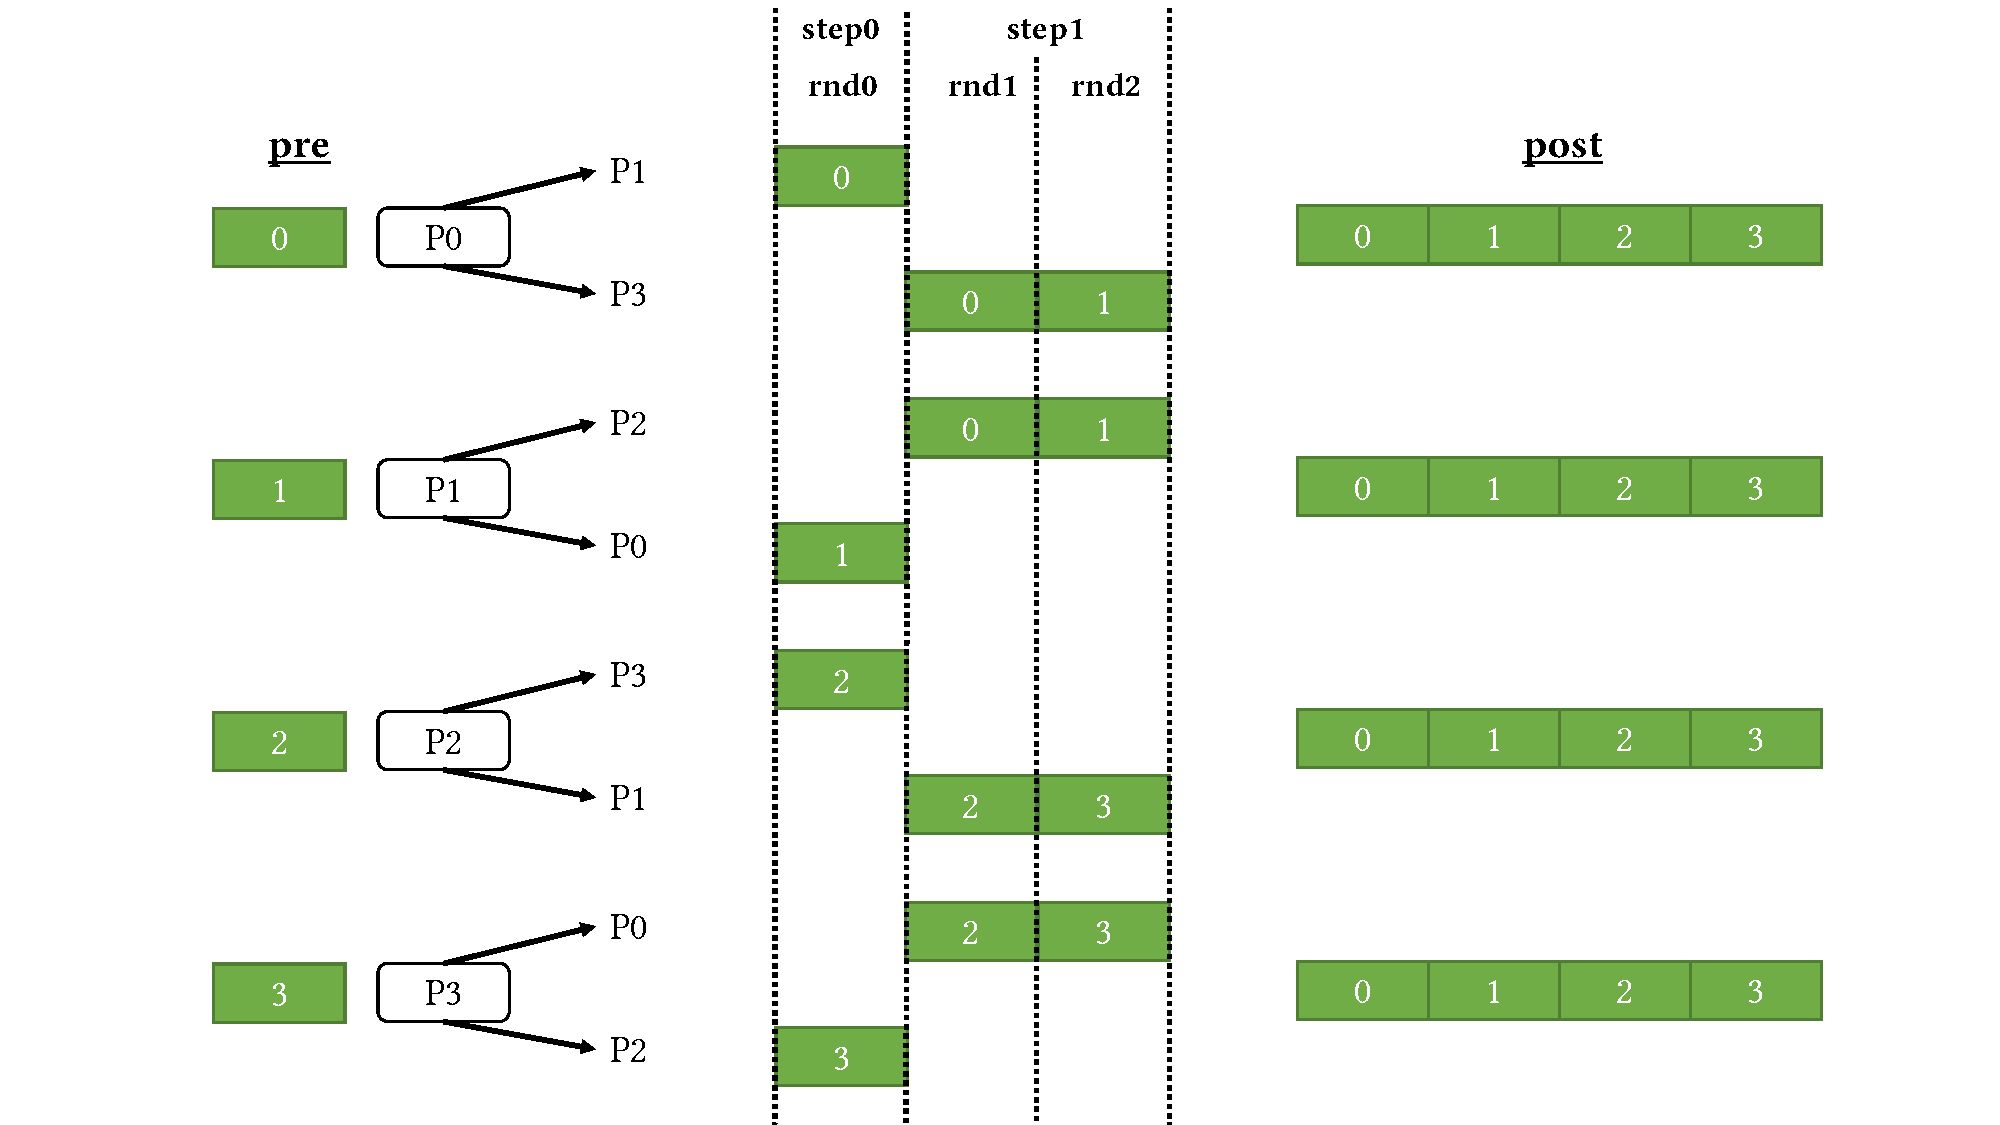
\includegraphics[width=\columnwidth]{figures/allgatherex.pdf}
    \caption{A $1$-synchronous algorithm for \allgather on a ring topology.}
    \label{fig:allgatherex}
\end{figure}

Figure~\ref{fig:allgatherex} shows the
recursive-doubling~\cite{thakur2005optimization} algorithm for
\allgather for a ring topology of four nodes $P0, P1, P2, P3$ with
four bidirectional links of equal bandwidth. This algorithm proceeds
in two {\em steps}. In the first step, nodes at "distance" 1, namely
$P0, P1$ and $P2, P3$ send their data to each other. Each node now has
data from two nodes, which it communicates entirely with nodes at
distance 2, i.e., nodes $P0, P3$ and $P1, P2$ in the second step. At
the end, each node has data from every other node. Since the second
step involves sending twice the amount of data as the first step, we
say it has two \emph{rounds} where in each round, it sends data. Thus,
this step has a total of $3$ rounds. Of the eight (unidirectional)
links, this algorithm uses only four of them per step. To improve
bandwidth utilization, a better option is to split the input data into
equal-sized {\em chunks} and communicate them independently. For
instance, the ring algorithm described in
Section~\ref{sec:motivation:bw-optimal} uses $3$ chunks per node.

The algorithm in Figure~\ref{fig:allgatherex} and many classical
collective algorithms~\cite{thakur2005optimization,chan2007collective}
are instances of {\em synchronous} algorithms. A synchronous algorithm
proceeds in a sequence of synchronous communication {\em steps} with
nodes waiting for other nodes to finish their rounds before starting
the next step. Even if an implementation might not enforce a global
barrier across the nodes, these algorithms choose the amount of data
to communicate per step based on the bandwidth constraints so that the
nodes finish each step at (roughly) the same time.

Many algorithms, like the one in Figure~\ref{fig:allgatherex},
communicate different numbers of chunks per step. We consider each
step as consisting of multiple rounds with each node sending at most
one chunk per unit-bandwidth on its outgoing links. Intuitively, the
number of rounds in an algorithm controls its bandwidth cost, while
the number of steps controls its latency cost. A synchronous algorithm
with $\steps$ steps and $\rounds$ rounds is {\em $k$-synchronous} if
$\rounds \leq \steps + k$. The parameter $k$ limits the amount of
communication per step and allows an SMT solver to effectively search
the space of algorithms bounded by that $k$.
%\todo{Madan mentioned in the chat that for a given $k$, we use it to
%bound $R$. We can make it clearer. The first time I read this, I
%thought we are changing $k$ for some $R$ and $S$ such that $k$ is the
%smallest number such that $R\le S+k$.}

%The terminology of steps and rounds might be confusing at first. The
%best way to distinguish them is to note that in the $(\alpha, \beta)$
%cost model, the latency cost of a $k$-synchronous algorithm depends
%on the number of steps, while the bandwidth cost depends on the
%number of rounds and the number of the chunks.

\subsection{\broadcastingCap Collective Instance}
Now we will provide a uniform formulation for representing
$k$-synchronous algorithms for \broadcasting collectives. An instance
of \collectiveproblem is a tuple
$(\gchunk,\steps,\rounds,\size,\bw,\pre,\post)$, where
\begin{itemize}
    \item[] \hspace{-0.5cm}Parameters:
    \begin{itemize}
    \item $\gchunk\in\posint$ is the global number of chunks
    \item $\steps\in\posint$ is the total number of steps
    \item $\rounds\in\posint$ is the total number of rounds
    \end{itemize}
    \item[] \hspace{-0.5cm}Topology:
    \begin{itemize}
    \item $\size\in\posint$ is the number of nodes
    \item
    $\bw\subseteq\powerset(\range{\size}\times\range{\size})\times\mathbb{N}$
    is the bandwidth relation
    \end{itemize}
    \item[] \hspace{-0.5cm} Specification:
    \begin{itemize}
        \item $\pre\subseteq\range{\gchunk}\times\range{\size}$ is the
        pre-condition
        \item $\post\subseteq\range{\gchunk}\times\range{\size}$ is
        the post-condition
    \end{itemize}
\end{itemize}
Note that for a set $M$ we write $\powerset(M)$ for the power set of
$M$, i.e., the set of all subsets. For an integer $x$, we write
$\range{x}$ for the set $\{0, 1, \ldots, x\}$. Here, $\gchunk, \steps,
\rounds$ are parameters to the desired $k$-synchronous algorithm. The
rest are explained below.

\subsubsection{Topology}
\label{sec:topology}
$\size$ is the number of nodes in the topology. $\bw$ gives a flexible
way to express different bandwidth constraints we have seen in
practice. In its most general form, $\bw$ bounds the sum of chunks
sent along a set of edges in a single round. A point-to-point
communication link from $s$ to $d$ with maximum bandwidth (in chunks
per round) $b$ can be modeled by $(\{(s, d)\}, b) \in \bw$. Some
topologies might limit the net outgoing bandwidth $b$ from a certain
node $s$. If $E$ is the set of outgoing neighbors of $s$, we can model
this by $(\{(s, e) \mid e \in E\}, b) \in \bw$. To model shared bus
topologies, where only one node can send in a round, we include
$(\{(a, b) \mid a \in N, b \in N\}, b)$ in $\bw$ for the set of nodes
$N$ sharing the same link. Note that these constraints are per round,
and when performing $r_i$ rounds in step $i$, we simply multiply the
bandwidth constraint by $r_i$.

\newcommand{\relAll}{All\xspace}
\newcommand{\relRoot}{Root\xspace}
\newcommand{\relScattered}{Scattered\xspace}
\newcommand{\relTranspose}{Transpose\xspace}
\newcommand{\chunkReduce}{\left\lfloor\frac{i}{\size}\right\rfloor}
\begin{table}
    \center
    \begin{tabularx}{\columnwidth}{@{}Xl@{}}
        \toprule
        Name & Relation \\
        \midrule
        \relAll & $\range{\gchunk}\times\range{\size}$ \\
        \relRoot & $\range{\gchunk}\times\{n_\mathit{root}\}$ \\
        \relScattered & $\{(c,n)\in\range{\gchunk}\times\range{\size}
        \setwhere n=c\bmod \size\}$ \\
        \relTranspose & $\{(c,n)\in\range{\gchunk}\times\range{\size}
        \setwhere n=\left\lfloor\frac{c}{\size}\right\rfloor\bmod
        \size\}$ \\
        \bottomrule
    \end{tabularx}
    \caption{Common relations in pre- and post-conditions of collective primitives.}
    \label{tbl:relations}
\end{table}
\begin{table}
    \begin{tabularx}{\columnwidth}{@{}Xll@{}}
        \toprule
        Collective & $\pre$ & $\post$ \\
        \midrule
        \gathercoll & \relScattered & \relRoot  \\
        \allgather & \relScattered & \relAll  \\
        \alltoall & \relScattered & \relTranspose  \\
        \broadcast & \relRoot & \relAll \\
        \scatter & \relRoot & \relScattered  \\
        \bottomrule
    \end{tabularx}
    \caption{Specifications of collective primitives.}
    \label{tbl:collectives}
\end{table}

\begin{comment}
    \begin{table}
    \begin{tabularx}{\columnwidth}{@{}Xlll@{}}
        \toprule
        Collective & $\pre$ & $\post$ & $\chunk(c)$ \\
        \midrule
        \gathercoll & \relScattered & \relRoot & $c$ \\
        \allgather & \relScattered & \relAll & $c$ \\
        \alltoall & \relScattered & \relTranspose & $c$ \\
        \broadcast & \relRoot & \relAll & $c$ \\
        \scatter & \relRoot & \relScattered & $c$ \\
        \reduce & \relScattered & \relRoot & $\chunkReduce$ \\[2pt] %
        make sure floor symbols don't stick together
        \allreduce & \relScattered & \relAll & $\chunkReduce$ \\[2pt]
        \reducescatter & \relScattered & \relTranspose &
        $\chunkReduce$ \\[2pt]
        \bottomrule
    \end{tabularx}
    \caption{Specifications of collective primitives as \collectiveproblem instances using a small set of common relations for pre- and post-conditions.}
    \label{tbl:collectives}
\end{table}
\end{comment}
\subsubsection{Collective Specification}
\label{sec:specifications}
The $\pre$ relation specifies the nodes where the chunks reside at the
beginning of the algorithm and the $\post$ relation specifies the set
of nodes where a chunk needs to be transferred to.
Table~\ref{tbl:relations} specifies useful relations that can be used
to specify common collectives as shown in Table~\ref{tbl:collectives}.
For instance, \allgather starts in a state where chunks are in the
\relScattered relation in Table~\ref{tbl:relations}. In other words,
the $c$ chunks of the input at node $n$ are given chunk identifier
$i\cdot P + n$ for $0 \leq i < c$. From this \relScattered state,
\allgather requires all the input chunks to be copied to all nodes, as
specified by \relAll relation in Table~\ref{tbl:relations}. Similarly,
\broadcast requires all the chunks from the root $n_{root}$ to be
copied to all nodes.

\begin{comment}
We have identified a small number of relations
(Table~\ref{tbl:relations}) that can be mixed-and-matched to model
most common collective primitives (Table~\ref{tbl:collectives}).
Collectives using \relRoot require that a root node $n_\mathit{root}$
has been given. The \relScattered relation is used in collectives that
evenly distribute input data onto nodes, and collectives that use it
require that $\chunk\bmod\size=0$ The \relTranspose relation is used
in conjunction with \relScattered to re-distribute scattered data, and
to ensure an even redistribution these collectives require that
$\chunk\bmod\size^2=0$.

\allreduce as it is specified in Table~\ref{tbl:collectives} needs an
associative reduction operation or else it can give different results
on different nodes. See Section~\ref{sec:background-collectives} for
more discussion.
\todo{Point this Section reference to where the allreduce discussion actually ends up at.}
\end{comment}

\begin{comment}
nodes each identifier starts from, while $\post$ specifies the nodes
that each identifier must end up on. For example, a point-to-point
send primitive with $\size=2$ and $\chunk=1$ might have
$\pre=\{(0,0)\}$ and $\post=\{(0,1)\}$. Note that the pre-condition
can specify that copies of an identifier start from multiple nodes,
which is not useful for traditional collectives. However, this feature
can be useful for specifying more exotic collectives for situations
where an application has already placed identical copies of data onto
some nodes.
\end{comment}

\begin{comment}
% Madan moved this to earlier

The bandwidth relation $\bw$ gives a flexible way to express various
kinds of networks. Topologies with direct links between a source node
$s$ and a destination node $d$ will have $\bw$ of the form
$\{(\{(s,d)\},b),(\{(s',d')\},b'),\dotscend\}$, where $b,b',\dotscend$
give the per link bandwidths. And, to limit the total outgoing
bandwidth from a node $n$ to be no more than $b$, may be modeled with
an entry of the form $(\{(n,n') \setwhere n'\in\range{\size}\},b)$. A
switch that all traffic between two sets of nodes $P$ and $Q$ can be
modeled with an entry of the form $(\{(n,n') \setwhere n\in P \wedge
n'\in Q\},b)$. See Section~\ref{sec:topologies} for details on how we
model the network topologies found in our hardware targets.
\end{comment}

\begin{comment}
The qouta relation $\qouta$ allows multiple chunks be sent in a step
through a link. A link with a bandwidth of $b$ can transfer $2b$
chunks in a 2 short steps which each transferring $b$ chunks but
alternatively the same link could transfer $2b$ chunks in a longer
step. This enables the synthesizer to find algorithm which are more
latency optimal.
\todofor{Olli}{Do we want to talk about sharing of nodes here? - this is important as most cross node topologies have shared interconnects in addition to PCIe}
\todofor{Olli}{our assumptions below  do not allow different sized chunks.  this is fine, but i wonder if we want to have a section on our ``asusmptions'' to push off potential challenges from reviewers.}
\end{comment}

\begin{comment}
% Madan: changed the example to allgather
As an example, consider the \reduce collective primitive, which
reduces data from all nodes onto a single root node $n_\mathit{root}$.
The target hardware will have some number of nodes $\size$ and
bandwidth relation $\bw$. To split the input data into $d$ chunks, the
number of identifiers is set to $\chunk=d*\size$. Now the problem of
synthesizing an algorithm can be modeled by setting:
\begin{align*}
    \pre&=\{(c,n)\in\range{\chunk}\times\range{\size} \setwhere n=c\bmod \size\} \\
    \post&=\range{\chunk}\times\{n_\mathit{root}\} \\
    \chunk(i)&=\left\lfloor\frac{i}{\size}\right\rfloor
\end{align*}
The pre-condition requires that identifiers are distributed onto nodes
in a round-robin fashion, while the post-condition requires all
identifiers to end up on the root node. $\chunk$ maps blocks of
$\size$ identifiers to the same chunk, thus reducing them together in
the result.
\end{comment}

While \collectiveproblem uses a global number of chunks $\gchunk$, it
is more typical in existing literature to consider the per-node number
of chunks $\chunk$. We will use the per-node number when discussing
the cost model and search algorithm in Sections~\ref{sec:costmodel}
and \ref{sec:pareto:optimal} and when presenting our evaluation in
Section~\ref{sec:evaluation}. Note that how these two counts relate to
each other is collective dependent: for \broadcast $\gchunk=\chunk$,
while for \allgather $\gchunk=\size\cdot\chunk$. The formalization
must still use a global numbering of chunks, as some exotic
collectives, e.g. MPI's Allgatherv, may not have a single per-node
chunk count.

\subsection{Candidate Solution}
Given an instance of \collectiveproblem
$(\gchunk,\steps,\rounds,\size,\bw,\pre,\post)$, a candidate solution
is a pair $(\rparts,\sends)$. Here $\rparts$ is a sequence
$r_0,\allowbreak r_1,\allowbreak \dotsc,\allowbreak r_{\steps -1}$
such that $\sum_i r_i = \rounds$ and denotes the number of rounds per
step. $\sends$ is a set of sends of the form $(c,n,n',s)$, which
specifies that chunk $c$ must be sent from node $n$ to node $n'$ at
step $s$. This defines a {\em run} defined as a  sequence
$V_0,V_1,\dotsc,V_{\steps}$ such that $V_0 = \pre$ and for all $0 \leq
s < \steps$, $V_{s+1}$ reflects the chunks present at a given node
after accounting for the sends at step $s$:
%$V_{\steps -1} \subseteq \post$
$$ V_{s+1} = V_{s} \cup \{(c,n') \mid (c, n) \in V_{s} \wedge (c, n,
n', s) \in \sends\} $$

This candidate solution is a valid $k$-synchronous algorithm for the
instance if $V_{\steps} \subseteq \post$ and the following bandwidth
constraint hold
\begin{align*}
    &\begin{aligned}
        \forall &s\in\range{\steps},\,(L,b)\in\bw \qst \\
        & |\{(c,n,n',s)\in \sends \setwhere (n,n')\in L\}|\leq b \cdot r_s
    \end{aligned}
\end{align*}
%\todo{introduce in the order of correctness constraints and bandwidth
%constraints. Sequence $Q$ can be explained together with the
%bandwidth constraints}
At each step $s$ consisting of $r_s$ rounds, the number of sends in
each link should be bounded by the bandwidth constraint multiplied by
$r_s$.
% \begin{align*} & \exists r_0, r_1, \ldotsc, r_{\steps-1} : \sum_i
%     r_i = \rounds \wedge \\
%     & \forall &t\in\range{\steps},\,(L,b)\in\bw \qst \\
%     & |\{(c,n,n',t)\in S \setwhere (n,n')\in L\}| \leq b \cdot r_i
% \end{align*}

\begin{comment}
\begin{align*}
    &V_0=\{(i,n,\Ite{(i,n)\in\pre}{1}{0}) \setwhere (i,n)\in\range{\chunk}\times\range{\size}\} \\
    &\begin{aligned}
        V_t=\{(i,n,\Sigma\{&r' \setwhere (i,n',r')\in V_{t-1} \wedge (n=n' \vee \\
        &(\chunk(i),n',n,t-1)\in S)\}) \setwhere (i,n)\in\range{\chunk}\times\range{\size}\}
    \end{aligned}
\end{align*}
Each $V_t$ has entries of the form $(i,n,r)$, which indicate that
identifier $i$ has reached node $n$ a total of $r$ times.
%
The candidate solution $S$ is an \emph{algorithm} for $P$ if and only
if the following conditions hold:
\begin{alignat}{3}
    &\mathrlap{ \forall (i,n,r)\in V_{\steps} \qst (i,n)\in\post
    \Rightarrow r=1} \tag{A1}\label{eqn:a1}\\
    &\begin{aligned} \forall &t\in\range{\steps},\,(L,b)\in\bw \qst \\
        &b\geq|\{(c,n,n',t)\in S \setwhere (n,n')\in L\}|
    \end{aligned} \tag{A2}\label{eqn:a2}
\end{alignat}
Condition~\ref{eqn:a1} ensures that the algorithm satisfies the
post-condition of the problem instance. Because reduction operations
are not always idempotent, Condition~\ref{eqn:a1} requires that each
identifier has contributed to the result exactly once.
Condition~\ref{eqn:a2} ensures that the bandwidth limitations are
respected by counting the number of sends happening on each time step
and checking that this is below the limit. Because we assume that all
chunks are the same size, \ref{eqn:a2} can simply compare the number
of sends to the bandwidth limit.
\end{comment}
%\subsection{Specifications for Common Collectives}
%\label{sec:specifications}


\subsection{SMT Encoding for \broadcastingCap Collectives}
\label{sec:encoding}
\begin{comment}
    While \collectiveproblem is amenable to a direct encoding into
    SMT, we choose to use an encoding for the special case of
    $\gchunk(i)=i$, i.e., the case where there is no reduction
    happening and each identifier corresponds to a unique chunk. We
    call these collectives \emph{broadcasting collectives}.
    Section~\ref{sec:reduction} will then show how the synthesis
    problem for a larger class of collectives that do perform
    reduction can be reduced to the synthesis problem for broadcasting
    collectives. The reduction reduces the number of identifiers,
    leading to better synthesis performance. Since we assume that
    $\gchunk(i)=i$ we use chunks and identifiers interchangeably in
    the following explanation.
\end{comment}
Given an instance, the SMT encoding incorporates the constraints above
allowing the SMT solver to systematically search over candidate
solutions $(\rparts, \sends)$. It is straightforward to encode each
$r_s$ of $\rparts$ as integer variables whose sum is $\rounds$. In
contrast, one has to be careful in encoding $\sends$. For instance,
our initial attempt to encode every tuple $(c, n, n', s) \in \sends$
as a Boolean variable was not successful, because Z3, the SMT solver
we used, did not solve larger problem instances fast enough. One way
we were able to scale Z3 is to use a careful combination of Boolean,
integer, and pseudo-Boolean constraints as we describe below.

We split the encoding of $\sends$ into integer variables $\start{c}{n}
\geq 0$, indicating the earliest step a chunk $c$ becomes available at
node $n$ and Boolean variables $\send{n}{c}{n'}$ determining whether a
node $n$ sends chunk $c$ to $n'$ (at any step).
\newcommand{\edges}{E}
To help with pruning the encoding, let $\edges=\{(n,n') \setwhere
\allowbreak \forall (L,b)\in\bw \qst (n,n')\in L \Rightarrow b > 0\}$,
i.e., the pairs of nodes with non-zero bandwidth between them.
Pseudo-Boolean constraints allow one to use Boolean variables as $0,1$
integers which we will use in the exposition below.

The following two constraints enforce the pre- and post-conditions:
%Now we describe the constraints required for the encoding. Chunks
%must have a starting time of zero on all associated nodes in the
%pre-condition. For each $(c,n_{\mathit{pre}})\in\pre$ add the
%following constraint:
\begin{align}
%    \forall (c,n) \in \range{\gchunk} \times \range{\size} (c,n) \in \pre &\equiv \start{c}{n}=0
    \forall (c,n) \in \pre \ \ \start{c}{n} &=0
    \tag{C1}\label{eqn:bc-zero} \\
    \forall (c,n) \in \post \ \ \start{c}{n}&\leq \steps
%    \start{c}{n_{\mathit{post}}}&\leq\steps
    \tag{C2}\label{eqn:bc-insteps}
\end{align}
If a chunk becomes available in a node, but is not part of the
precondition, then the node should have received the chunk from some
other node. For optimality, we also enforce that the node does not
redundantly receive the chunk more than once.
%For each $(c,n)\in(\range{\ids}\times\range{\size})\setminus\pre$ add
%the following constraint:
\begin{align}
    \forall (c,n) \not\in \pre \ \ \start{c}{n}&\leq \steps \Rightarrow \Sigma_{(n',n)\in\edges}\,\send{n'}{c}{n}=1
    \tag{C3}\label{eqn:bc-hassender}
\end{align}
To send a chunk, it must exist on the source node before it is
received on the destination node.
%For each chunk $c\in\range{\ids}$ and pair of connected nodes
%$(n,n')\in\edges$ add the following constraint:
\begin{align}
    \forall (c,n) \in E \ \ \send{n}{c}{n'}\Rightarrow\start{c}{n}<\start{c}{n'}
%    \send{n}{c}{n'}\Rightarrow\start{c}{n}<\start{c}{n'}
    \tag{C4}\label{eqn:bc-sendexisting}
\end{align}
%Constraints \ref{eqn:bc-zero}, \ref{eqn:bc-insteps},
%\ref{eqn:bc-hassender} and \ref{eqn:bc-sendexisting} would be
%sufficient to satisfy Condition~\ref{eqn:a1}.
The following enforces the bandwidth constraint at all steps $1 \leq s
\leq \steps$ and bandwidth constraint $(L,b)\in\bw$:
%To satisfy Condition~\ref{eqn:a2}, we must ensure that the bandwidth
%limitations of the topology are respected. For each step of the
%algorithm $1 \leq t \leq \steps$ and bandwidth constraint
%$(L,b)\in\bw$ add the constraint:
\begin{align}
    \Sigma_{(c,(n,n'))\in\range{\gchunk}\times L}\left(\send{n}{c}{n'}\wedge\start{c}{n'}=s\right)\leq b \cdot r_s
    \tag{C5}\label{eqn:bc-bw}
\end{align}
%
Note, we have multiplied the bandwidth constraints by $r_s$ to allow
$r_s$ rounds at step $s$.
%
Finally, the following bounds the total rounds $\rounds$:
\begin{align}
    \Sigma_{1\leq s\leq\steps}(r_s)=\rounds
    \tag{C6}\label{eqn:bc-rounds}
\end{align}

%\begin{comment}
Once the problem instance has been encoded, the SMT solver will
attempt to find a model $M$, which maps the variables $\start{c}{n}$,
$\send{n}{c}{n'}$ and $r_s$ to concrete values such that Constraints
\ref{eqn:bc-zero} through \ref{eqn:bc-rounds} are satisfied. If a
model exists then an algorithm $(\rparts, \sends)$ can be constructed
with:
\begin{align*}
    \rparts&=M(r_0),\dotsc,M(r_{\steps-1}) \\
    \sends&=\{(c,n,n',t) \setwhere M(\send{n}{c}{n'}) \wedge M(\start{c}{n}) = t+1 \}
\end{align*}
If the SMT solver says the problem is unsatisfiable, then no algorithm
exists for the problem instance.
%\end{comment}


\subsection{\reducingCap Collectives}
\label{sec:reduction}
It is well known that certain \reducing collectives are {\em inverses}
of \broadcasting collectives. For instance, a \reduce algorithm can be
generated by inverting an algorithm for \broadcast on a topology where
all links have been reversed. Intuitively, whenever the \broadcast
sends the same chunk to two different nodes, in its inverse the
\reduce algorithm will receive the two {\em versions} of the chunk
from these nodes and apply the reduction operation. The node will send
the resulting chunk to the node it received the chunk from in the
\broadcast. Similarly, we can generate \reducescatter algorithms by
inverting \allgather algorithms. %For space reasons, we do not
describe the formal procedure of inverting \broadcasting collectives.

Generally the inverting procedure works for any \reducing collective
that has a single root node for each chunk. Notably, this does not
include \allreduce, which replicates the result onto all nodes. For
synthesizing \allreduce algorithms, we first notice that \allreduce
can be expressed as a combination of \reducescatter followed by an
\allgather. We synthesize \allreduce algorithms by synthesizing an
\allgather algorithm and preceding it with its inverse \reducescatter
algorithm.

\begin{comment}
While the SMT encoding presented in the previous section could be
extended to handle the general case, a direct encoding would require
tracking staring times per-identifier instead of per-chunk. For the
reducing collectives in Section~\ref{sec:specifications} this would
inflate the number of $\start{i}{n}$ variables by a factor of $\size$.
However, it turns out that for a class of reducing collectives that
reduce each chunk onto a unique node the synthesis problem can be
reduced to the subclass for broadcasting collectives. The special case
of turning an algorithm for \allgather into one for \reducescatter
with a symmetric bandwidth relation is well-known. This section
presents a generalized reduction, that handles any collective in this
class on any kind of topology.

\newcommand{\chunktochunk}{\mathcal{T}}
\newcommand{\algtoorig}{\mathcal{R}}

The reduction involves transforming pre- and post-con\-di\-tions such
that there is one identifier for each unique chunk. Given any post- or
pre-condition $R$, we use the following function to perform this
transformation:
\[
    \textstyle
    \chunktochunk(R) = \{(c,n) \setwhere \exists (i,n)\in R \qst \chunk(i)=c \}
\]
Let $P=(\size,\bw,\chunk,\chunk,\pre,\post,\steps)$ be an instance of
\collectiveproblem such that the following condition holds:
\begin{gather}
    % \chunk\bmod\size=0 \tag{R1}\\
    % \chunk(i)=\chunkReduce \tag{R2}\\
    \forall (i,n),(i',n')\in\post \qst \chunk(i)=\chunk(i') \Rightarrow n=n' \tag{SR}\label{eqn:single-root}
\end{gather}
Out of the collectives in Table~\ref{tbl:collectives} this condition
holds for \reduce and \reducescatter, but not for \allreduce. The
reason is that the post-condition is required to give a unique root
node for each set of identifiers that correspond to the same chunk,
but \allreduce reduces each chunk onto all nodes.

Additionally, without loss of generality, we assume that the set of
chunks $\{\chunk(i) \setwhere i\in\range{\chunk}\}$ forms a continuous
integer interval starting from zero. Any $P$ not satisfying this can
be transformed to this form by remapping $C$.

Now construct a new instance of \collectiveproblem as
$P'=(\size,\allowbreak\bw',\allowbreak\chunk',\allowbreak\chunk',\allowbreak\pre',\allowbreak\post',\allowbreak\steps)$
where:
\begin{gather*}
    \bw'=\{(L',b) \setwhere (L,b)\in\bw \wedge L'=\{(n',n) \setwhere (n,n')\in L\} \} \\
    \chunk'=|\{\chunk(i) \setwhere i\in\range{\chunk}\}| \hspace{2em} \chunk'(i)=i \\
    \post'=\chunktochunk(\pre) \hspace{2em} \pre'=\chunktochunk(\post)
\end{gather*}
Let $\algtoorig$ be a function for mapping algorithms for $P'$ back to
$P$ defined as follows:
\[
    \algtoorig(S')=\{ (c,n',n,\steps-t-1) \setwhere (c,n,n',t)\in S' \}
\]
\begin{theorem}
    Given an algorithm $S'$ for $P'$, the transformed solution
    candidate $S=\algtoorig(S')$ is an algorithm for $P$.
    \label{thm:reduction-solution}
\end{theorem}
    \begin{proof}
    % A sequence of sends
    % $(a_0,n_0,n'_0,t_0),\dotsc,(a_{m-1},n_{m-1},n'_{m-1},t_{m-1})$
    % in a solution candidate is a \emph{path} (of length $m$) if
    % $\forall i\in\range{m} \qst $

    Given an identifier $i$ the sequences of nodes $n_0,\dotsc,n_m$
    and steps $t_0,\dotsc,t_{m-1}$ form a \emph{path} from $n_0$ to
    $n_m$ in a solution candidate $S''$ if $\forall k\in\range{m} \qst
    (\chunk(i),n_k,n_{k+1},t_k)\in S''$ and $\forall k\in\range{m-1}
    \qst t_k < t_k+1 \wedge 0 \leq t_k \leq \steps-1$.

    %There is a unique starting node for each chunk in $P'$.
    Because \ref{eqn:single-root} holds for $P$, then for each
    identifier $i\in\range{chunks}$ there exists a unique
    $(i,n_{\mathit{root}})\in\post$ and thus, due to the way
    $\chunktochunk$ collapses identifier of the same chunk into a
    single identifier, a unique
    $(\chunk(i),n_{\mathit{root}})\in\pre'$. Now since \ref{eqn:a1}
    holds for $S'$, for each $(i,n)\in\post'$ there exists a unique
    path from $n_{\mathit{root}}$ to $n$ in $S'$, as otherwise the
    count for $(i,n)$ in $V'_\steps$ would not be 1.

    Due to the way $\algtoorig$ flips the sources and destinations of
    sends and also reverses their ordering in time, each path in $S'$
    from a node $n$ to another node $n'$ corresponds to a path from
    $n'$ to $n$ in $S$. Thus for each $(i,n)\in\pre$ there exists a
    unique path from $n$ to $n_{\mathit{root}}$. Therefore,
    \ref{eqn:a1} holds for $S$.

    Because \ref{eqn:a2} holds for $S'$ and both $\bw'$ and
    $S=\algtoorig(S')$ flip the order of sources and destinations,
    then \ref{eqn:a2} holds also for $S$, which therefore is an
    algorithm for $P$.
\end{proof}

\begin{theorem}
    If no algorithm exists for $P'$ then there are no algorithms for
    $P$ either.
    \label{thm:reduction-no-solution}
\end{theorem}
    The proof for Theorem~\ref{thm:reduction-no-solution} takes a
    similar form to the proof for
    Theorem~\ref{thm:reduction-solution}.
\begin{proof}
    Assume there exists an algorithm $S$ for $P$. Since \ref{eqn:a1}
    holds for $S$, for each $(i,n)\in\pre$ there exists a unique path
    from $n$ to $n_{\mathit{root}}$ (see proof of
    Theorem~\ref{thm:reduction-solution} for explanation of
    $n_{\mathit{root}}$).

    Let $S'=\algtoorig(S)$. Given that $\algtoorig$ flips sources and
    destinations of sends as well as reverses their stepwise ordering,
    each path in $S$ corresponds to a reversed path in $S'$. Thus for
    each $(i,n)\in\post'$ there exists a unique path from
    $n_{\mathit{root}}$ to $n$. Therefore, \ref{eqn:a1} holds for $S'$

    Because \ref{eqn:a2} holds for $S$ and both $\bw'$ and
    $S=\algtoorig(S')$ flip the order of sources and destinations,
    then \ref{eqn:a2} holds also for $S'$, which therefore is an
    algorithm for $P$. This is a contradiction. Thus the assumption
    that $S$ is an algorithm for $P$ is false and the original theorem
    is true.
\end{proof}

Now for any instance of \collectiveproblem for which
\ref{eqn:single-root} holds this reduction can be used to transform it
into a form that the SMT encoding in Section~\ref{sec:smt-encoding}
can be used. If a solution exists then $\algtoorig$ can be used to get
a solution to the original instance. If no solution exists, then there
is no solution to the original instance either.
\end{comment}

\subsection{Cost Model}
\label{sec:costmodel}
Say we have synthesized a $k$-synchronous algorithm with $\chunk$
chunks, $\steps$ steps, and $\rounds$ rounds. We will use the
$(\alpha, \beta)$ cost model~\cite{hockney1994communication} to
evaluate cost of this algorithm. Here, $\alpha$ is the latency of each
link in the topology and $\beta$ is the time taken sending a byte
along a unit-bandwidth link. If the input data of $L$ bytes is divided
into $\chunk$ chunks, a step $s$ with $r_s$ rounds takes $\alpha +
\frac{r_s}{\chunk}\cdot L \cdot \beta$ time. Therefore, the entire
algorithm will finish in time
$$ \steps \cdot \alpha + \frac{\rounds}{\chunk} \cdot L \cdot \beta. $$
%In effect, one can reduce the latency cost by reducing the number of
%steps, and reduce the bandwidth cost either by increasing the number
%of chunks or decreasing the number of rounds.

\subsection{Pareto-optimal Algorithms}
\label{sec:pareto:optimal}
The discussion above shows that for a given topology and a collective
with an input size $L$, the cost of a $k$-synchronous algorithm can be
characterized by the tuple $(\steps, \frac{\rounds}{\chunk})$. An
algorithm with cost $(a,b)$ is {\em Pareto-optimal} with respect to
the class of $k$-synchronous algorithms if for every algorithm in this
class with cost  ($a', b')$ we have $a = a' \Rightarrow b' \geq b$ and
$b = b' \Rightarrow a' \geq a$. An algorithm with cost $(a,b)$ is
considered {\em latency-optimal} ({\em bandwidth-optimal}), if for
every $k$-synchronous algorithm with cost $(a',b')$ we have $a' \geq
a$ ($b' \geq b$).

Note that latency- or bandwidth-optimal algorithms are not necessarily
Pareto-optimal as they can be "wasteful" in the other parameter.
Pareto-optimal algorithms form a {\em Pareto-frontier} with different
algorithms in the frontier being better than others for a given input
size $L$ based on the $\alpha$ and $\beta$ parameters of the topology.

Algorithm~\ref{alg:pareto} systematically synthesizes Pareto-optimal
$k$-synchronous algorithms. The inputs are the parameter $k$, the name
of the collective to synthesize, and the topology parameters $\size,
\bw$~(Section~\ref{sec:topology}). The procedure computes the latency
lower bound $a_l$ from the diameter of the topology, and the bandwidth
lower bound $b_l$ from the inverse bisectional bandwidth of the
topology. The procedure starts enumerating steps $\steps$ starting
with $a_l$. Then it generates $A$, the candidate set of tuples
$(\rounds, \chunk)$ that satisfy the round constraint and the inverse
bandwidth constraint. Note that without the $k$ parameter, this set
would be unbounded. The procedure checks if a
$(\steps,\rounds,\chunk)$ algorithm exists in the increasing order of
the bandwidth cost $\frac{\rounds}{\chunk}$ using the encoding
discussed in Section~\ref{sec:encoding}. If one exists, the reported
algorithm is guaranteed to be Pareto-optimal for the current steps
$\steps$. As we increase the number of $\steps$, we get algorithms
with lower bandwidth cost. Additionally, if the current bandwidth cost
matches the lower bound $b_l$, the procedure returns. As we have
already generated the Pareto-optimal algorithm with $b_l$ bandwidth
cost, it is not necessary to increase $\steps$ further. Note, that it
is possible for this procedure to never terminate as there can
sometimes be unbounded number of Pareto-optimal algorithms for certain
topologies and collectives. While the synthesis procedure above is for
\broadcasting collectives, synthesis for \reducing collectives is
similar~(Section~\ref{sec:reduction}).
%\todo{explains that when increase $S$, we should have better $(R,C)$
%pairs for better bandwidth. The limit the to the bandwidth is the
%lower bound, once we can reach it, there's no point increasing $S$,
%because it increases the latency.}


\begin{algorithm}
	\caption{Synthesizing Pareto-Optimal Algorithms}
    \label{alg:pareto}
    \begin{algorithmic}[1]
        \Procedure{Pareto-Synthesize}{$k, \mathit{Coll}, \size, \bw$}
        \State $a_l = \mathit{Diameter(\size, \bw)}$ \State $b_l =
        \mathit{InvBisectionBandwidth(\size, \bw)}$ \State $(\pre,
        \post) = \mathit{Lookup(Coll)}$
        \Comment{Table~\ref{tbl:collectives}} \For
        {$\steps=a_l,a_l+1\ldots$} \State $A = \{(\rounds,\chunk) \mid
        \steps \leq \rounds \leq \steps+k \wedge
        \frac{\rounds}{\chunk} \geq b_l\}$ \For {$(R,\chunk) \in A$ in
        ascending order of $\frac{R}{\chunk}$} \State
        $\gchunk=\toglobal(\mathit{Coll},\chunk)$ \If
        {$\mathit{SMT(\gchunk, \steps, \rounds, \size, \bw, \pre,
        \post) = SAT}$} \State Report synthesized algorithm
        $(\steps,\rounds,\chunk)$ \If {$\frac{\rounds}{\chunk} = b_l$}
        \State {\bf return} \EndIf \State {\bf break} \EndIf \EndFor
        \EndFor \EndProcedure
	\end{algorithmic}
\end{algorithm}

\section{Code Generation}
\label{sec:lowering}
The prior section described a synthesis procedure for generating
Pareto-optimal algorithms. This section describes a tool called
\tool{} that implements this procedure and generates high-performance
collective implementations for both NVIDIA and AMD GPUs.


Every synthesized algorithm, at its core, is a sequence of commands
that describe \emph{what} data needs to be sent (i.e., which chunk),
\emph{where} it needs to be sent (i.e., a source and destination),
\emph{when} it needs to be sent (i.e., during which synchronous step),
and \emph{with} which chunk(s) it needs to be reduced. \tool{}
generates SPMD multi-process \CC{} code combined with CUDA kernels
that implement these commands.

Each GPU involved in the computation has its own code as part of a
top-level switch statement. Communication between GPUs is enabled
using CUDA IPC memory handles, which allows a GPU to access a remote
GPU's memory using shared pointers. Thus, communication between GPUs
simply involves writing data to appropriate buffers. However, there
are a few crucial choices that impact the communication performance.

%This mechanism chooses the fastest available hardware transport when
%there are multiple connections available. For example, on a \dgxone,
%NVLink will be used by default to communicate between GPUs; otherwise
%PCIe may be used. On the Gigabyte Z52 consisting of AMD GPUs, xGMI
%will be used for GPUs in the same ring; otherwise PCIe will be used.
%Section~\ref{sec:evaluation} describes the details.

%\subsection{Hardware Interconnects and the Software that uses them}
% Before we discuss how we generate code, we first enumerate the
% possible ways for GPUs to communicate with each other in modern
% hardware.

%\subsection{Interconnect usage details}

%Once the memory handles between connected GPUs are exchanged, there
%are multiple ways to enable data transfers.

\subsection{DMA Engines and Kernel Copies:} Data may be moved either by
executing load or store instructions through a kernel, or by using a
specialized DMA engine via \texttt{cudaMemcpy}. A kernel copy allows
data movement and computation to be fused in a kernel while a DMA
engine has a higher initial $\alpha$ cost but may have higher
bandwidth, leading to a lower $\beta$ cost. On NVLink, DMA engine
bandwidth is about 10\% better than kernel copy bandwidth, due to
details of the wire-level protocol. Transfers are packetized, with
each packet including a header (containing address, error correction
data, etc.) and a variable-length payload. DMA engines are able to
emit maximum-sized packets, but kernel copy packets are limited to the
128-byte cache line size.

\subsection{Push and Pull Models:} Each DMA engine is located on a
particular GPU. Data movement between two GPUs can be executed by
either the receiver's DMA engine (a {\em pull} model) or by the
sender's DMA engine (a {\em push} model). Kernel copies have the same
two approaches. This may have performance implications due to the link
protocol: the push model only needs to send write request packets with
a payload, whereas a pull model first sends request packets and then
receives response packets with data. When communicating
bidirectionally, the request packets reduce the bandwidth available
for the response packets. Thus, even though the push model may require
extra memory, we have found it to be up to 10\% faster than the pull
model.

%Furthermore, when a \reducing collective receives chunks, it can
%reduce immediately after the receiver pulls the data whereas in the
%push model, the reduction can be computed lazily right before the
%reduced chunk is sent. Thus,

%Our experiments suggest that the push model is faster than pull.

\subsection{Single and Multiple Kernels:} One way to implement a
synthesized algorithm is by emitting several kernels, one per step,
which forces a global synchronization between steps and, as a
consequence, introduces large overheads. Alternatively, \tool{} fuses
all steps into one kernel and thus we implement the synchronizations
between GPUs as a fine-grained signal and wait mechanism with shared
flags. In our single kernel implementation, each chunk for each
connection has a dedicated flag; a chunk on a GPU is valid only when
the associated flag is set. There is a
\texttt{\_\_threadfence\_system()} between the data movement
operations and the operation to set the flag on the remote GPU signals
that the transfer is complete.

\subsection{Size and Number of Thread Blocks:} \tool{} dedicates a
given number of thread blocks to each link and for each step, it uses
the same number of thread blocks to communicate through that link. For
different input sizes, the number of thread blocks significantly
affects performance and in later sections we show how we empirically
search for the fastest configuration for various input sizes.

% \paragraph{CPU or GPU?} Data movement between the CPU's memory and
% the GPU's memory may be done either by the GPU or the CPU. Using the
% GPU is common: the same tradeoffs discussed above apply. The CPU's
% memory is mapped into the GPU's address space; when a DMA engine or
% load/store instruction accesses that region, the GPU's memory system
% generates read or write operations over the PCIe bus. It is also
% possible to map the GPU's memory into the CPU's address space and
% use load/store instructions on the CPU to access the GPU's memory;
% this is the goal of the GDRCopy library~\cite{gdrcopy}. Since these
% transfers do not need to pay the GPU kernel invocation cost, their
% latency can be lower than GPU-initiated transfers; however, because
% the GPU cannot be prefetched, the bandwidth is low compared to
% GPU-managed transfers.

% \paragraph{Framing overhead} One challenge in determining whether a
% communication scheme is using a link efficiently is determining what
% data transfer bandwidth to expect. Manufacturers often report link
% speeds in terms of raw bit rate, but once link framing overhead is
% taken into account, the rate at which user data is transferred will
% be lower.

% For instance, an NVLink 2.0 link as found on the V100 has a raw
% unidirectional bandwidth of just over 25 GB/s~\cite{nvlink2}.
% However, NVLink communication is structured in terms of 16-byte
% flits; each packet contains between one and three header flits
% (containing address, operation, acknowledgment, error correction,
% and other information), and up to 16 data flits~\cite{nvlink1}.
% Thus, the user-visible bandwidth will always be lower than 25 GB/s.
% The choice between using DMA engines or kernel copies affects this:
% the DMA engines are able to emit maximum-sized packets and thus we
% see a user-visible bandwidth of about 22 GB/s; for kernel copies the
% packets are limited to the 128-byte cache line size, leading to a
% user-visible bandwidth of about 20 GB/s.

% The other interconnects found in our configurations have similar
% properties. We omit the protocol details here. AMD's xGMI (Infinity
% Fabric) interconnect on the MI50 has a raw bit rate of 46
% GB/s~\cite{mi50}, and the peak link bandwidth we observe is
% approximately 33 GB/s. The PCIe 3.0 x16 links on the NVIDIA
% configurations have a raw bandwidth of 16 GB/s, but we measure a
% peak bandwidth of about 14 GB/s. The PCIe 4.0 links on the AMD
% configuration has a raw bandwidth of 32 GB/s, and we measure a peak
% bandwidth of about 27.5 GB/s.

% \todofor{Todd}{Explain general code generation approach, producing
% CUDA C++, general structure of generated code} \subsection{GPU to
% GPU Communication Methods}

% \todofor{Jacob}{Enumerate and explain all the different ways to
% communicate between GPUs. cudaMemcpy, kernel pull/push, gdrcopy etc.
% Performance considerations and tradeoffs between these.}

% \todofor{Saeed}{Explain which GPU to GPU communication methods we
% chose and how we implemented them.}

% \subsection{Lowering}

% \paragraph{Targeting PCIe}: \tool{} generates code driven by the
% CPU. Memory involved in a collective is pinned.  When possible, we
% exploit NUMA effects to register pinned memory on the socket that
% owns it.  We exploit gdrcopy\cite{gdrcopy} for low-latency transfers
% over PCIe of this pinned memory.  We extend gdrcopy to also enable
% reduction operations as the current codebase only supports send/recv
% and not addition as required in, for example, an Allreduce.  Because
% pinning memory is expensive, we cache pointers to buffers used in
% collectives.


% \subsection{Lessons in Low-level Communication Optimizations}

% \todofor{Zhengyang}{Enumerate all the system hacks that went in.}

%%% Local Variables: %% mode: latex %% TeX-master: "paper" %% End:


\section{Evaluation}
This section demonstrates how we model and synthesize collectives for
two multi-GPU systems with proprietary interconnects used for training
large deep learning models. In both cases, we demonstrate 1) how to
model the interconnect using \tool, 2) what transport we utilize in
lowering synthesized collectives, and 3) the Pareto-frontier of
algorithms we find for the respective interconnects.

\subsection{Hardware}
The following section describes the hardware topology we model for our
NVIDIA and AMD machines.

\subsubsection{NVIDIA DGX-1: 8 V100 GPUs}
A DGX-1 is a multi-GPU server sold directly by NVIDIA in addition to
being a pay-as-you-go rental option in most cloud providers.  It
contains two 20-core Intel Xeon E5-2698 v4 processors with 512 GB DRAM
split across the two sockets, along with 8 NVIDIA V100 GPUs, each with
32 GB of HBM2 memory. The GPUs are connected using NVIDIA's
proprietary NVLink interconnect; each GPU has 6 25 GB/s NVLink ports.
Figure~\ref{fig:dgx1-topo} shows the topology: the 8 GPUs are
interconnected with 2 non-overlapping Hamiltonian cycles.  One of
those cycles has two NVLink connections between each pair of GPUs. The
GPUs are also connected to the CPUs by PCIe 3.0 x16 links, but we do
not use them due to the wide disparity between per-GPU NVLink and PCIe
bandwidth ($\sim$150~GB/s vs. $\sim$14~GB/s). We also run synthesis on
this platform.

\begin{figure}
\includegraphics[page=2,width=\columnwidth]{figures/topos}
\caption{Topology of a Gigabyte MI50 8 GPU AMD System.}
\label{fig:amd-topo}
\end{figure}

\subsubsection{Gigabyte Z52: 8 AMD MI50 GPUs}
A Gigabyte Z52 system is a consumer grade multi-GPU system. It has two
64-core AMD EPYC 7002 processors with 1 TB DRAM split across the two
sockets, as well as 8 AMD MI50 GPUs, each with 32 GB of HBM2 memory. 4
GPUs are connected to each socket with PCIe links, denoted by a box in
Figure~\ref{fig:amd-topo}. Like NVIDIA, AMD also provides a
proprietary high-speed interconnect called xGMI that links GPUs
together.  Each blue line is an xGMI link between a pair of GPUs. Note
that the xGMI connections build two disconnected islands: 3 GPUs per
island are on 1 socket while a lone GPU is on the \emph{other} socket
(i.e., GPU 1 and 5). The Gigabyte system uses PCIe 4.0 x16 links with
measured bandwidth ($\sim$27 GB/s) that approaches xGMI's measured
bandwidth ($\sim$33 GB/s). As such, we use PCIe to connect the rings.

\subsection{Modeling Bandwidth Constraints}
The hardware in this chapter has distinct and interesting topologies.
This section describes how we model those respective topologies in
\tool.

\subsubsection{NVIDIA DGX-1: 8 V100 GPUs}
Each NVLink connection is point-to-point; thus our bandwidth
constraints are simply the enumeration of each pair of GPUs connected
via NVLink. As each NVLink connection can send 1 chunk per round,
$\bw$ has entries $(\{(n,n')\},1)$ for each pair of GPUs in one cycle
and entries $(\{(n,n')\},2)$ for GPUs in the other.

\subsubsection{Gigabyte Z52: 8 AMD MI50 GPUs}
Unlike NVLink, xGMI connections are not simply point-to-point but also
transparently act as a router.  For example, GPU 2 can send a message
to GPU 3 even though they lack a physical connection: GPU 0 routes
messages on GPU 2's behalf.  However, this utilizes multiple links,
and thus if GPU 0 concurrently sends a message to GPU 3, it can expect
half the bandwidth of the link.  We thus only model the direct
connections in Figure~\ref{fig:amd-topo}.  One way to connect the
rings is to utilize PCIe and let GPU 1 connect to all other GPUs
within its same socket (0, 2, and 3) and GPU 5 connect to GPUs within
its same socket (4, 6, and 7).  Because PCIe is shared, we could also
enforce that only 1 PCIe connection occurs on every round, per socket.
%
% remove if need space
For example, the entry in $\bw$ for the left socket is
$(\{(0,1),(1,0),(1,2),(2,1),(1,3),(3,1)\},1)$.
%
However, we were unable to utilize both xGMI and PCIe at the same time
so our model of the bandwidth ignores the dotted xGMI connections in
Figure~\ref{fig:amd-topo}.  As such, we explicitly model the topology
as a ring with GPUs 1 and 5 connecting the xGMI islands. Lastly,
because the bisection bandwidth between the two xGMI islands is
limited by the PCIe links that connect them, any bandwidth optimal
algorithm will be limited by the bandwidth of these PCIe links.
Therefore, we model the same $\beta$ cost for xGMI and PCIe and assume
all links can send a single chunk per step.
%Finally, we noticed a single kernel was not able to utilize both xGMI
%and PCIe at the same time so we restrict each GPU to using only two
%of the potentially three possible links.


\subsection{NCCL and RCCL Baselines}
We use NCCL (version 2.7.8-1) and RCCL (installed from ROCm 3.5.0) for
baselines on NVIDIA and AMD hardware, respectively.  NCCL is a
hand-written and optimized communication library from NVIDIA. RCCL is
a port of NCCL that uses the ROCm HIP compiler and targets AMD
hardware. They share the same core algorithms and differ only in how
they interact with the underlying hardware.

\newcolumntype{H}{>{\setbox0=\hbox\bgroup}c<{\egroup}@{}}

\begin{table}[bp]
\caption{NCCL hand-written collectives and their chunks and steps. }
\begin{tabularx}{\columnwidth}{@{}Xlll@{}}
\toprule
Collective &$\chunk$ & $\steps$ & $\rounds$ \\
\midrule
\allgather/\reducescatter & 6 & 7 & 7 \\
\allreduce & 48 & 14 & 14 \\
\broadcast/\reduce  & $6m$ & $6+m$ & $6+m$ \\
\bottomrule
\end{tabularx}

\label{table:nccl}
\end{table}

Table~\ref{table:nccl} gives an overview of the collectives that NCCL
implements and number of chunks and steps they use on a \dgxone.
NCCL's algorithms are all based on either rings or trees. However,
Table~\ref{table:nccl} uses only ring algorithms, as we observed that
on DGX-1 NCCL's trees are just simple paths, which are no better than
using rings for any input size.
% As of NCCL version 2.8.7-1, the tree based algorithm is only used in
% \allreduce and upon manual inspection, the tree on our \dgxone node
% is actually a ring.

Our analysis of the chunks ($\chunk$), steps ($\steps$), and
rounds($\rounds$) is from our manual inspection of the NCCL source.
For \reduce and \broadcast NCCL implements a pipelined algorithm,
which chooses a multiplier $m$ such that chunks stay approximately
equally sized. Their running times are then $(6+m) \cdot \alpha +
\frac{6+m}{6m}\cdot L \cdot \beta$ and they get closer to bandwidth
optimality as $m$ gets larger.

As we show in the next section, \tool{} is able to synthesize all
these NCCL collectives and more, including \scatter, \gathercoll, and
\alltoall.
%Further, for each collective, \tool{} synthesizes many more
%Pareto-optimal algorithms.

% synhtesis looks fast but it is solving a hard problem and our
% results are due to efforts noted above.  Naive encoding does not
% scale... maybe remove some symmetry?

\subsection{Synthesizing Collective Algorithms}
Table~\ref{fig:dgxone:syn} and Table~\ref{fig:amd:syn} enumerate
various algorithms we synthesize for NVIDIA \dgxone and Gigabyte's
\amd architecture.  For each collective, we synthesize a latency and
bandwidth optimal implementation, along with others that exist at
various points along the latency-bandwidth curve. The first column
combines collectives which are the inverse of each other (i.e.,
\scatter and \gathercoll) and those that can be reduced to the
\broadcasting collective using the reduction explained in
Section~\ref{sec:reduction} (e.g. \reduce to \broadcast).

\subsubsection{Optimality}
Note we find many latency and bandwidth optimal algorithms for each
collective, as we search over $k$-synchronous algorithms for different
values of $k$. Consider the \allgather collective: we find many
algorithms with various numbers of steps. However, the latency optimal
algorithms (2 steps) dominate all others in the $\alpha$ term of the
cost model.  Likewise, the bandwidth optimal algorithms dominate all
others with their low ratio of rounds to chunks ($7/6$). We
synthesized algorithms in the $0$-synchronous class ($\rounds =
\chunk$) as the code generation is much easier.

%There are various reasons to synthesize more than the lowest latency
%bandwidth-optimal and highest bandwidth latency-optimal algorithms:
%for example, any algorithm with $R == S$ is straightforward to
%implement as each step has a logical barrier between them.

Note that NCCL's \allgather algorithm is bandwidth optimal, and while
it is also the lowest latency algorithm that NCCL provides, it is not
latency optimal. We are able to synthesize both a bandwidth optimal
algorithm with better latency (6-chunks 3-steps 7-rounds), as well as
a latency optimal algorithm. In general, our synthesized latency
optimal algorithms have no counterpart in NCCL and our bandwidth
optimal algorithms are better than NCCL's for \allgather, \broadcast,
and \reduce.

%See Section~\ref{sec:pareto:optimal} for a discussion of how latency
%and bandwidth optimality relate to Pareto-optimality.

\begin{table}[tbp]
\caption{\dgxone collectives with chunks ($\chunk$), steps ($\steps$) and rounds ($\rounds$).  }
\begin{tabularx}{\columnwidth}{@{}lHlllXHr@{}}
\toprule
Collective & Topology & $\chunk$ & $\steps$ & $\rounds$ & Optimality &
Running Time & Time \\
\midrule
\allgather & \dgxone & 1 & 2 & 2 &Latency&$2 \cdot \alpha + 2\cdot L
\cdot \beta$& 0.3 s\\
(\reducescatter)& \dgxone & 2 & 3 & 3 &&$3 \cdot \alpha + 3/2\cdot L
\cdot \beta$& 0.8 s\\
 & \dgxone & 3 & 4 & 4 &&$4 \cdot \alpha + 4/3\cdot L \cdot \beta$&
 1.5 s\\
 & \dgxone & 4 & 5 & 5 &&$5 \cdot \alpha + 5/4\cdot L \cdot \beta$&
 2.3 s\\
 & \dgxone & 5 & 6 & 6 &&$6 \cdot \alpha + 6/5\cdot L \cdot \beta$&
 3.3 s\\
 & \dgxone & 6 & 7 & 7 &Bandwidth&$7 \cdot \alpha + 7/6\cdot L \cdot
 \beta$& 4.6 s\\
 & \dgxone & 6 & 3 & 7 &Bandwidth&$3 \cdot \alpha + 7/6\cdot L \cdot
 \beta$& 6.6 s\\
 & \dgxone & 2 & 2 & 3 &Latency&$2 \cdot \alpha + 3/2\cdot L \cdot
 \beta$& 0.9 s\\
\hline
\allreduce & \dgxone & 8  &4  &4&Latency&$4 \cdot \alpha + 1/2\cdot L
\cdot \beta$& 0.3 s\\
  & \dgxone & 16 &6  &6&&$6 \cdot \alpha + 3/8\cdot L \cdot \beta$&
  0.6 s\\
  & \dgxone & 24 &8  &8&&$8 \cdot \alpha + 1/3\cdot L \cdot \beta$&
  1.3 s\\
  & \dgxone & 32 &10 &10&&$10 \cdot \alpha + 5/16\cdot L \cdot \beta$&
  2.9 s\\
  & \dgxone & 40 &12 &12&&$12 \cdot \alpha + 3/10\cdot L \cdot \beta$&
  5.6 s\\
  & \dgxone & 48 &14 &14&Bandwidth&$14 \cdot \alpha + 7/24\cdot L
  \cdot \beta$& 12.8 s\\
  & \dgxone & 48 &6  & 14&Bandwidth&$6 \cdot \alpha + 7/24\cdot L
  \cdot \beta$& 23.0 s\\
  & \dgxone & 16 &4  &6&Latency&$4 \cdot \alpha + 3/8\cdot L \cdot
  \beta$& 0.8 s\\
\hline
\broadcast & \dgxone & 2 & 2 & 2 &Latency&$2 \cdot \alpha + 1\cdot L
\cdot \beta$& 0.1 s\\
(\reduce) & \dgxone & 6 & 3 & 3 &&$3 \cdot \alpha + 1/2\cdot L \cdot
\beta$& 0.3 s\\
 & \dgxone & 12 & 4 & 4 &&$4 \cdot \alpha + 1/3\cdot L \cdot \beta$&
 1.0 s\\
 & \dgxone & 18 & 5 & 5 &&$5 \cdot \alpha + 5/18\cdot L \cdot \beta$&
 8.5 s\\
 & \dgxone & 6 & 3 & 5 &&$3 \cdot \alpha + 5/6\cdot L \cdot \beta$&
 0.9 s\\
\hline
\gathercoll & \dgxone & 1 & 2 & 2 &Latency&$2 \cdot \alpha + 2\cdot L
\cdot \beta$& 0.3 s\\
(\scatter) & \dgxone & 2 & 3 & 3 &&$3 \cdot \alpha + 3/2\cdot L \cdot
\beta$& 0.9 s\\
  & \dgxone & 3 & 4 & 4 &&$4 \cdot \alpha + 4/3\cdot L \cdot \beta$&
  1.6 s\\
  & \dgxone & 4 & 5 & 5 &&$5 \cdot \alpha + 5/4\cdot L \cdot \beta$&
  2.7 s\\
  & \dgxone & 5 & 6 & 6 &&$6 \cdot \alpha + 6/5\cdot L \cdot \beta$&
  3.8 s\\
  & \dgxone & 6 & 7 & 7 &Bandwidth&$7 \cdot \alpha + 7/6\cdot L \cdot
  \beta$& 6.0 s\\
  & \dgxone & 6 & 3 & 7 &Bandwidth&$3 \cdot \alpha + 7/6\cdot L \cdot
  \beta$& 11.4 s\\
  & \dgxone & 2 & 2 & 3 &Latency&$2 \cdot \alpha + 3/2\cdot L \cdot
  \beta$& 1.0 s\\
\hline
\alltoall & \dgxone & 8 & 3 & 3 &&$3 \cdot \alpha + 3/8\cdot L \cdot
\beta$& 2.6 s\\
  & \dgxone & 8 & 2 & 3 &Latency&$2 \cdot \alpha + 3/8\cdot L \cdot
  \beta$& 3.0 s\\
  & \dgxone & 24 & 8 & 8 &Bandwidth&$8 \cdot \alpha + 1/3\cdot L \cdot
  \beta$& 133.7 s\\
  & \dgxone & 24 & 2 & 8 &Both&$2 \cdot \alpha + 1/3\cdot L \cdot
  \beta$& 24.3 s\\
\bottomrule
\end{tabularx}

%For \reducescatter and \scatter $\chunk$ should be multiplied by 8.
\label{fig:dgxone:syn}
\end{table}

\begin{table}[tbp]
  \caption{\amd collectives with chunks ($\chunk$), steps ($\steps$) and rounds ($\rounds$). }
  \begin{tabularx}{\columnwidth}{@{}lHlllXHr@{}}
\toprule
Collective & Topology & $\chunk$ & $\steps$ & $\rounds$ & Optimality &
Running Time & Time \\
\midrule
\allgather & \amd & 1 & 4 & 4 &Latency&$4 \cdot \alpha + 4\cdot L
\cdot \beta$& 0.5 s\\
(\reducescatter) & \amd & 2 & 7 & 7 &Bandwidth&$7 \cdot \alpha +
7/2\cdot L \cdot \beta$& 1.3 s\\
 & \amd & 2 & 4 & 7 &Both&$4 \cdot \alpha + 7/2\cdot L \cdot \beta$&
 1.7 s\\
\hline
\allreduce & \amd & 8 &8&8&Latency&$8 \cdot \alpha + 1\cdot L \cdot
\beta$& 0.4 s\\
 & \amd & 16 &14&14&Bandwidth&$14 \cdot \alpha + 7/8\cdot L \cdot
 \beta$& 0.9 s\\
 & \amd & 16 &8&14&Both&$8 \cdot \alpha + 7/8\cdot L \cdot \beta$& 1.6
 s\\
\hline
\broadcast & \amd & 2 & 4 & 4 &Latency&$4 \cdot \alpha + 2\cdot L
\cdot \beta$& 0.1 s\\
(\reduce) & \amd & 4 & 5 & 5 &&$5 \cdot \alpha + 5/4\cdot L \cdot
\beta$& 0.2 s\\
 & \amd & 6 & 6 & 6 &&$6 \cdot \alpha + 1\cdot L \cdot \beta$& 0.3 s\\
 & \amd & 8 & 7 & 7 &&$7 \cdot \alpha + 7/8\cdot L \cdot \beta$& 0.5
 s\\
 & \amd & 10 & 8 & 8 &&$8 \cdot \alpha + 4/5\cdot L \cdot \beta$& 0.6
 s\\
\hline
\gathercoll & \amd & 1 & 4 & 4 &Latency&$4 \cdot \alpha + 4\cdot L
\cdot \beta$& 0.4 s\\
(\scatter) & \amd & 2 & 4 & 7 &Both&$4 \cdot \alpha + 7/2\cdot L \cdot
\beta$& 1.8 s\\
\hline
\alltoall & \amd & 8 & 4 & 8 &Both&$4 \cdot \alpha + 1\cdot L \cdot
\beta$& 8.2 s\\
\bottomrule
\end{tabularx}
%For \reducescatter and \scatter $\chunk$ should be multiplied by 8.
\label{fig:amd:syn}
\end{table}


\subsubsection{Synthesizing All Collectives}
Collective communication libraries need to support a large and diverse
set of hardware architectures.  Efficiently implementing latency and
bandwidth optimal algorithms for various topologies is time-consuming
and error-prone. \tool's synthesis based approach allows it to easily
extend the set of algorithms through search: \tool{} synthesizes
algorithms for \alltoall, \gathercoll and \scatter where no such
counterparts exist in NCCL.

\subsubsection{Synthesis Time}
The longest synthesis time is just over 2 minutes and most of the time
under 10 seconds.  The synthesis problem is non-trivial and its
complexity is defined by both the collective, as well as the hardware
topology we synthesize for. The clever encoding described in
Section~\ref{sec:encoding} was critical for achieving these fast
synthesis times. As a point of comparison, synthesizing the 24-chunk
8-step bandwidth-optimal \alltoall algorithm with a more direct
encoding with a Boolean variable for each tuple $(c, n, n', s) \in
\sends$ did not finish within 60 minutes. With the better encoding the
synthesis finishes in just over 2 minutes.

\subsection{Performance Evaluation}
In this section, we compare \tool's generated algorithms with NCCL and
RCCL on the NVIDIA and AMD hardware.  Our code generation uses a
protocol similar to the simple protocol (i.e., NCCL\_PROTO=Simple).
Thus, we use NCCL with the simple protocol as our baseline. We
investigate the performance of \allgather, \allreduce, and \alltoall
as they are popular primitives in different workloads including
machine learning. For each hardware platform and collective, we
generate multiple algorithms; for each algorithm, we lower using (1) a
single kernel-launch, or (2) multiple \texttt{cudaMemcpy} calls with
one per step. Each algorithm uses a push model for copying and when
\tool{} is compared with NCCL, we exhaustively search the size and the
number of thread blocks and report the best performing combination for
both \tool{} and NCCL. See Section~\ref{sec:lowering} for more
details.

\begin{figure}[tbp]
  \centering
  \subfloat[Average latency\label{fig:dgx1-res-allgather-avglat}]{
    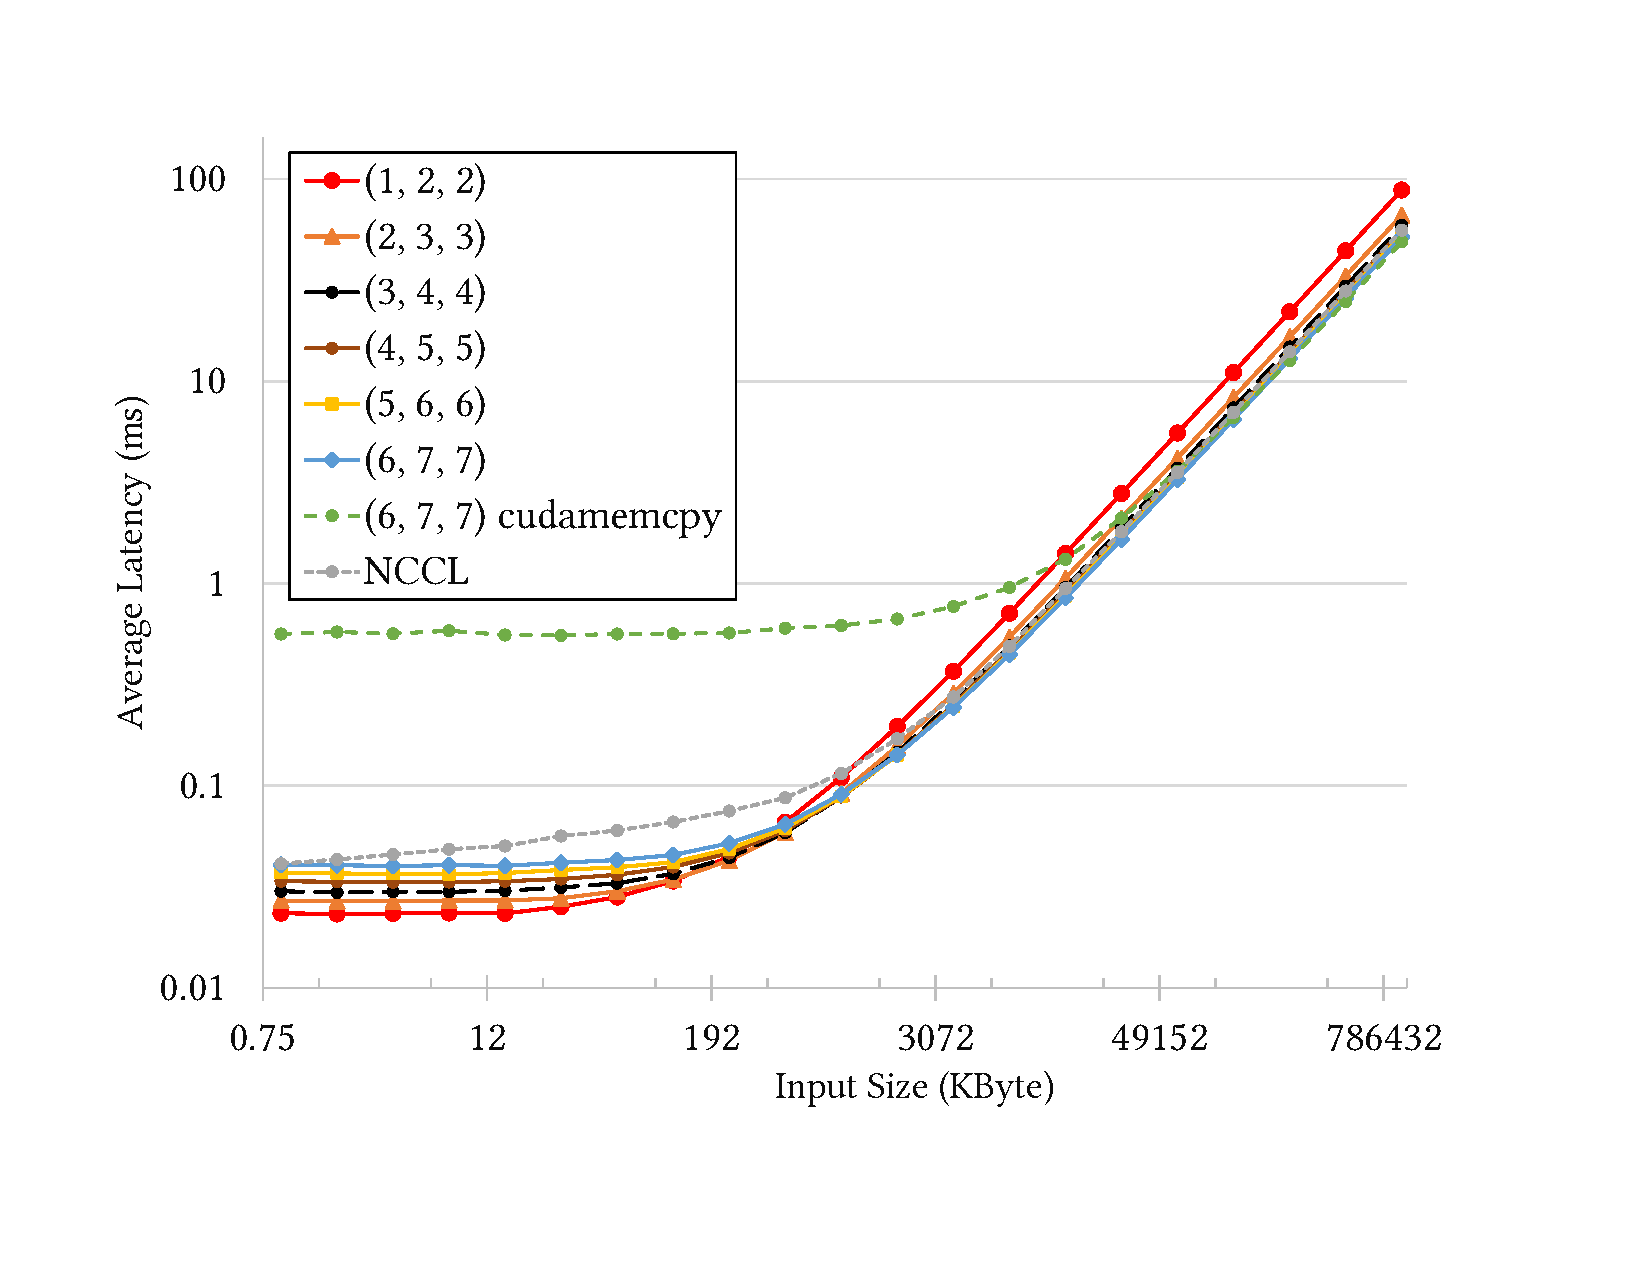
\includegraphics[page=1,width=0.84\columnwidth]{figures/evals-camera-ready}
  }
  \hfill
  \subfloat[Speedup\label{fig:dgx1-res-allgather-speedup}] {
    \includegraphics[page=2,width=0.84\columnwidth]{figures/evals-camera-ready}
  }
  \caption{\allgather performance comparison with NCCL.}
  \label{fig:dgx1-res-allgather}
\end{figure}

Figure~\ref{fig:dgx1-res-allgather} compares \tool's generated code
for \allgather with NCCL's \allgather. A point on
Figure~\ref{fig:dgx1-res-allgather-avglat} ($x$,$y$) shows the running
time in $y$ milliseconds as a function of send input buffer size in
$x$ Kbytes while a point on
Figure~\ref{fig:dgx1-res-allgather-speedup} shows the $y$ speedup of
\tool's generated code over NCCL's \allgather as a function of send
input buffer size in $x$ Kbytes. We plot one line per algorithm
denoted as $(\chunk, \steps, \rounds)$ for respectively chunks, steps,
and rounds as defined in Table~\ref{fig:dgxone:syn}. To show the
impact of our lowering, we plot two versions of a bandwidth optimal
algorithm $(6,7,7)$ (which utilizes a push-copy) and $(6,7,7)$
\texttt{cudaMemcpy}.  The latter of which shows the significant impact
lowering can have on the performance. To simplify the figure, we only
show algorithms that were faster on at least one input size we
experimented with. As it can be seen from the lines, \tool{} is up-to
$2.2\times$ faster than NCCL's \allgather on small sizes and
$1.14\times$ faster on larger sizes. It is possible for \tool{} to
automatically switch between multiple implementations based on the
input size. In which case, \tool{} will consistently outperform NCCL.

\begin{figure}[tbp]
  \centering
  \subfloat[Average latency\label{fig:dgx1-res-allreduce-avglat}] {
    \includegraphics[page=3,width=0.84\columnwidth]{figures/evals-camera-ready}
  }
  \hfill
  \subfloat[Speedup\label{fig:dgx1-res-allreduce-speedup}] {
    \includegraphics[page=4,width=0.84\columnwidth]{figures/evals-camera-ready}
  }
  \caption{\allreduce performance comparison with NCCL.}
  \label{fig:dgx1-res-allreduce}
\end{figure}


Likewise, Figure~\ref{fig:dgx1-res-allreduce} shows the running time
in milliseconds (Figure~\ref{fig:dgx1-res-allreduce-avglat}) or
speedup (Figure~\ref{fig:dgx1-res-allreduce-speedup}) for \allreduce
as a function of the receive input size.  Each line denotes $(\chunk,
\steps, \rounds)$ for respectively chunks, steps, and rounds,
respectively. With the exception of $4$ middle sizes, \tool{} beats
NCCL's \allreduce with an 8-chunk algorithm for small input sizes by
up-to $1.8\times$ and with a 48-chunk algorithm for large input sizes
by up-to $1.06\times$.

\alltoall is a complex algorithm which is very difficult to write
efficiently by hand. Unlike the prior collectives, NCCL does not
natively support \alltoall; instead, NCCL suggests using $N$
point-to-point exchanges (for $N$ GPUs) and thus its resulting
algorithm is neither bandwidth nor latency optimal.  Because \tool{}
uses program synthesis to generate optimal algorithms, it is able to
synthesize three \alltoall{} algorithms in a matter of minutes.
Figure~\ref{fig:dgx1-res-alltoall-avglat} shows the latency in
milliseconds of \tool{} and NCCL as a function of input size while
Figure~\ref{fig:dgx1-res-alltoall-speedup} shows speedup over NCCL
again as a function of input size.  Each line denotes $(\chunk,
\steps, \rounds)$ for respectively chunks, steps, and rounds and
demonstrates a speedup of over $6.8\times$ for large input sizes and
over $1.4\times$ for small input sizes, depending on whether we pick a
latency or bandwidth optimal implementation from \tool.  This
significant speedup really shows off the power of \tool's automated
approach to building algorithms tailored specifically to a hardware
architecture.

\begin{figure}[tbp]
  \centering
  \subfloat[Average latency\label{fig:dgx1-res-alltoall-avglat}]{
    \includegraphics[page=5,width=0.84\columnwidth]{figures/evals-camera-ready}
  }
  \hfill
  \subfloat[Speedup\label{fig:dgx1-res-alltoall-speedup}] {
    \includegraphics[page=6,width=0.84\columnwidth]{figures/evals-camera-ready}
  }
  \caption{\alltoall performance comparison with NCCL.}
  \label{fig:dgx1-res-alltoall}
\end{figure}

Lastly, we demonstrate \allgather on the Gigabyte AMD workstation.
Like the other plots, a point on Figure~\ref{fig:amd-res-allgather}
($x$,$y$) shows the latency or speedup $y$ for \allgather as a
function of the receive input size in bytes $x$.  We plot two
algorithms, $(1,4,4)$ and $(2,7,7)$; it is clear that (i) the lower
latency algorithm $(1,4,4)$ is better at smaller input sizes, (ii) the
higher bandwidth algorithm $(2,7,7)$ is faster for large input sizes,
and (iii) \tool's generated code is faster than RCCL for large sizes
but slower for medium and small sizes. The Gigabyte machine, in
particular, is new hardware and \tool{} can synthesize new algorithms
and implementations for it; this shows \tool{} can help design future
interconnects and co-design them with communication libraries.

These graphs in concert show that \tool{} is able to synthesize
algorithms along the Pareto-optimal frontier and also lower than to
hardware so as to be competitive with a hand optimized baseline.

\begin{figure}[tbp]
  \centering
  \subfloat[Average latency\label{fig:amd-res-allgather-avglat}]{
    \includegraphics[page=7,width=0.84\columnwidth]{figures/evals-camera-ready}
  }
  \hfill
  \subfloat[Speedup\label{fig:amd-res-allgather-speedup}] {
    \includegraphics[page=8,width=0.84\columnwidth]{figures/evals-camera-ready}
  }
  \caption{\allgather performance comparison with RCCL.}
  \label{fig:amd-res-allgather}
\end{figure}


\section{Related Work}
The message passing interface (MPI)~\cite{dongarra2013mpi} is a widely-used standardized abstraction for communication primitives in a multi processor system. Implementations of MPI provide reliable and portable implementations of collective primitives. Efficient algorithms for implementing these primitives is a long-studied research area~\cite{pjevsivac2007performance, chan2007collective, thakur2005optimization}, including optimized algorithms for specific architectures like mesh, hypercube, or fat-tree\cite{scott1991efficient,bokhari1992complete,barnett1993global} and for clusters of shared-memory processors~\cite{sistare1999optimization,traff2002improved,sanders2002hierarchical,tipparaju2003fast}. The class of $k$-synchronous algorithms studied in this paper is designed to include many of the algorithms proposed in these works and implemented in popular MPI implementations such as MPICH~\cite{thakur2005optimization} and OpenMPI~\cite{gabriel2004open}.

We evaluated OpenMPI, either through builtin CUDA capability or through Unified Communication X~(UCX)~\cite{ucx}.
They lack custom implementations for architectures such as the \dgxone{}, and result in subpar performance compared with our NCCL baselines.
NCCL~\cite{nccl} is a library for multi NVIDIA GPU systems and it utilizes the underlying hardware transport such as NVLink, NVSwitch or Infiniband for an efficient implementation of collective primitives. RCCL~\cite{rccl} is a port of NCCL for AMD GPUs and the HIP compiler suite. While these libraries provide efficient implementations for a limited set of algorithms, \tool{} is able to synthesize a wide range of algorithms suitable for different input sizes and generate collective primitives that are not even a part of standard MPI set.

There are also hybrid algorithms~\cite{barnett1994building, chan2007collective} that switch between latency- and bandwidth-optimal algorithm along each dimension of a mesh network. However, to the best of our knowledge, these prior works do not seek to identify algorithms that are Pareto-optimal for a given topology. In contrast to these prior works, the goal of this paper is to automatically synthesize Pareto-optimal algorithms for a given topology.  

There are also hierarchical approaches to implement collective primitives in distributed systems. Horovod~\cite{alex2018horovod} implements collective primitives by using NCCL locally in node and MPI across nodes. Others such as BlueConnect~\cite{blueconnect} and PLink~\cite{plink} exploit the hierarchical network topology of a cloud system or a data center to improve the performance of collective primitives. In this paper, we focus on synthesizing algorithms for a single node with multiple GPU, while the above approaches are beneficial on multi node systems.

Motivated by recent resurgence in machine-learning workloads, recent research has focused on optimizing the communication of distributed machine learning. Blink~\cite{wang2020blink}, the closest to our work, automatically synthesizes bandwidth-efficient collective primitives for a given topology. This work is based on packing spanning trees and is suitable for one-to-many collective primitives such as broadcast and reduce, and implements \allreduce as a reduce followed by a broadcast. Blink is not guaranteed to generate bandwidth-optimal algorithms as it heuristically selects a few trees based on an approximate spanning-tree packing algorithm. Moreover, Blink's focus is not on generating latency-optimal algorithms. In contrast, this work generates latency- and bandwidth-optimal algorithms for a given topology. There are also other works~\cite{zhang2017poseidon,hashemi2019tictac,jayarajan2019priority,peng2019generic} on optimizing distributed machine learning that do so by overlapping computation and communication and are orthogonal to this work. 

%\todo{Compare to related work on synthesizing compute kernels. Orthogonal.}

%\todo{Compareasd to related work on pipelining compute and communication. Orthogonal.} 

%%% Local Variables:
%%% mode: latex
%%% TeX-master: "paper"
%%% End:

\section{Conclusion}
This chapter introduces \tool: a systematic method to synthesize
algorithms in the Pareto-frontier spanning from the latency-optimal
algorithm to the bandwidth-optimal algorithm for a given collective on
an input topology. We characterize a class of algorithms that captures
a broad set of known algorithms and prove Pareto-optimality of both
known algorithms and synthesized new algorithms. We automatically
generate an implementation of these algorithms that is competitive
with manually hand-tuned communication kernels in use today.

\chapter{Conclusion}
\label{chap:conclusion}

This section concludes the thesis by summarizing the contributions.
%
The work established in this thesis is done on two different optimization
domains: peephole generation and collective communication synthesis.
%
The thesis that this dissertation has supported is that program synthesis can
be used to generate optimized and verifiable code for novel architectures.


This dissertation introduced \minotaur{}, a SIMD-oriented
superoptimizer that automatically
 generates peephole optimizations for LLVM IR code.
%
\minotaur{} has been shown to discover optimizations that are missed by
commodity compilers, and has demonstrated speedups on a variety of
benchmarks.

This dissertation also proposed SCCL, a syntheizer that generates
optimal collective communication algorithms a given hardware topology.
%
SCCL synthesizes algorithms along the Pareto-frontier spanning from
latency-optimal to bandwidth-optimal implementations of a collective.
%
The algorithm generated by SCCL are competitive with hand-optimized
collective communication libraries.


I hope that this work will inspire future research in the area of program
synthesis for performance optimization.


% % \numberofappendices = 1   % Set 0 for none, else number of appendices.
% \numberofappendices = 3
% \appendix       % Chapters, sections are now appendix style A, A.1, A.2, B, C, D, ...

% %%% -*-LaTeX-*-

\chapter{The First}

This is an appendix.  Notice that the \LaTeX{} markup for an appendix
is, surprisingly, \verb=\chapter=.  The \verb=\appendix= command does
not produce a heading; instead, it just changes the numbering style
from numeric to alphabetic, and it changes the heading prefix from
\textbf{CHAPTER} to \textbf{APPENDIX}.

\blah \blah \blah

% %%% -*-LaTeX-*-

\chapter{The Second}

This is an appendix.

\blah \blah \blah

% %%% -*-LaTeX-*-

\chapter{The Third}

This is an appendix.

There are several books
\cite{%
    Singh:1997:FEE,%
    Salomon:1995:AT,%
    Robbins:2005:CSS,%
    Randell:1982:ODC,%
    Olver:2010:NHM,%
    Mittelbach:2004:LC,%
    Lamport:1985:LDP,%
    Knuth:1999:DT,%
    Knuth:1986:TB,%
    Knuth:1986:MB,%
    Farmelo:2009:SMH%
}
listed in our bibliography.

We also reference several journal articles
\cite{%
    Wiles:1995:MEC,%
    Taylor:1995:RTP,%
    Lahiri:2002:ADA,%
    Kim:1999:AFC,%
    Johnson:1978:LDT,%
    Huskey:1980:LLC,%
    Heilbron:1969:GBA,%
    Hall:1994:PNE,%
    Goldstine:1946:ENI,%
    Einstein:1911:BMAb,%
    Einstein:1911:BMAa,%
    Einstein:1906:NBM,%
    Cody:1981:APF,%
    Beebe:1989:PCP,%
    Babbage:1910:BBA%
}
and three famous doctoral theses of later winners
\cite{%
    Einstein:1905:NBM,%
    Dirac:1926:QM,%
    Bohr:1911:SME%
}
of the Nobel Prize in Physics (1922, 1933, and
1921):

Notice that, even though those citations appeared
in \LaTeX{} \verb=\cite{...}= commands with their
\BibTeX{} citation labels in reverse alphabetical
order, thanks to the \verb=citesort= package,
their reference-list numbers have been sorted in
numerically ascending order, and then
range-reduced.

Mention should also be made of a famous Dutch
computer scientist's first publication
\cite{Dijkstra:1953:FBV}.

Font metrics are an important, albeit low-level,
aspect of typesetting. See the \emph{Adobe
Systems} manual about that company's procedures
\cite{Adobe:1990:AFM}.

The bibliography at the end of this thesis contains several examples
of documents with non-English titles, and their \BibTeX{} entries
provide title translations following the practice recommended by the
American Mathematical Society and SIAM\@.  Here is a sample entry that
shows how to do so:
%
\begin{verbatim}
@PhdThesis{Einstein:1905:NBM,
  author =       "Albert Einstein",
  title =        "{Eine Neue Bestimmung der Molek{\"u}ldimensionen}.
                 ({German}) [{A} new determination of molecular
                 dimensions]",
  type =         "Inaugural dissertation",
  school =       "Bern Wyss.",
  address =      "Bern, Switzerland",
  year =         "1905",
  bibdate =      "Fri Dec 17 10:46:57 2004",
  bibsource =    "http://www.math.utah.edu/pub/tex/bib/einstein.bib",
  note =         "Published in \cite{Einstein:1906:NBM}.",
  acknowledgement = ack-nhfb,
  language =     "German",
  advisor =      "Alfred Kleiner (24 April 1849--3 July 1916)",
  URL =          "http://en.wikipedia.org/wiki/Alfred_Kleiner",
  remark =       "Received August 19, 1905 and published February 8,
                 1906.",
  Schilpp-number = "6",
}
\end{verbatim}

The \texttt{note} field in that entry refers to another bibliography
entry that need not have been directly cited in the document text.
Such cross-references are common in \BibTeX{} files, especially for
journal articles where there may be later comments and corrigenda that
should be mentioned.  Embedded \verb=\cite{}= commands ensure that
those possibly-important other entries are always included in the
reference list when the entry is cited.  The last bibliography entry
\cite{Wiles:1995:MEC} in this thesis has a long \texttt{note} field
that tells more about what some may view as the most important paper
in mathematics in the last century.

When entries cite other entries that cite other entries that cite
other entries that \ldots{}, multiple passes of \LaTeX{} and \BibTeX{}
are needed to ensure consistency.  That is another reason why document
compilation should be guided by a \texttt{Makefile} or a batch script,
rather than expecting the user to remember just how many passes are
needed.

\BibTeX{} entries are \emph{extensible}, in that arbitrary key\slash
value pairs may be present that are not necessarily recognized by any
bibliography style files.  The \texttt{advisor},
\texttt{acknowledgement}, \texttt{bibdate}, \texttt{bibsource},
\texttt{language}, \texttt{remark}, and \texttt{Schilpp-number} fields
are examples, and may be used by other software that processes
\BibTeX{} entries, or by humans who read the entries.  \texttt{DOI}
and \texttt{URL} fields are currently recognized by only a few styles,
but that situation will likely change as publishers demand that such
important information be included in reference lists.

In \BibTeX{} \texttt{title} fields, braces protect words, such as
proper nouns and acronyms, that cannot be downcased if the selected
bibliography style would otherwise do so.  In German, all nouns are
capitalized, and the simple way to ensure their protection is to brace
the entire German text in the title, as we did in the entry above.

The world's first significant computer program may
have been that written in 1842 by Lady Augusta Ada
Lovelace (1815--1852) for the computation of Bernoulli
numbers \cite{Huskey:1980:LLC,Kim:1999:AFC}.  She
was the assistant to Charles Babbage
(1791--1871), and they are the world's first
computer programmers. The programming language
\emph{Ada} is named after her, and is defined in
the ANSI/MIL-STD-1815A Standard; its number
commemorates the year of her birth.

We do not discuss mathematical \emph{transforms}
in this dissertation, but you can find that phrase
in the index (except that this sample thesis doesn't have one!)

\blah

\blah
\blah

\blah


%%% The choice of bibliography style is a major decision, jointly made
%%% by you, your thesis advisor and the thesis editor. Common choices are
%%% one of the four standard BibTeX styles (abbrv, alpha, plain, and unsrt),
%%% or enhanced styles like acm, amsplain, siam, and hundreds of others
%%% available in TeX Live, and other Unix and Windows TeX distributions.
%%%
%%% Do NOT handcode your reference list, because you are unlikely to
%%% achieve consistency or conformance to the University of Utah Thesis Office
%%% requirements: let BibTeX do that tedious job for you!
%%%
%%% Remember that reference-list metadata in BibTeX files remains
%%% constant across journals and publishers, and is are often reused
%%% in other documents and shared with others, whereas formatted
%%% reference-list styles change: with BibTeX, you only need to record
%%% the metadata once.
%%%
%%% If you prefer named, rather than numeric or tagged citations, you
%%% may use styles such as authordate{1,2,3,4}, chicago, harvard, or
%%% natbib.  Be aware, however, that most of those require an
%%% additional \usepackage{} command to supply \LaTeX{} with
%%% definitions of commands that the style needs, and that there are
%%% usually several flavors of LaTeX citation commands beyond the
%%% standard \cite{} command that you need to understand before you
%%% can use them properly in your prose.

%%% This tells BibTeX to read siam.bst from the first directory where
%%% it is found in the BSTINPUTS search path:

\bibliographystyle{siam}

%%% This can also specify a comma-separated list (without embedded
%%% spaces) of *.bib files found by BibTeX in its BIBINPUTS search
%%% path.  The argument \jobname means the base name of the top-level
%%% LaTeX file, avoiding an unnecessary filename dependence here.
%%%
%%% BibTeX writes only one .bbl file, no matter how many *.bib files
%%% are listed here, using the name \jobname.bbl.
%%%
%%% LaTeX reads BibTeX's formatted reference list from the file
%%% \jobname.bbl.

\bibliography{\jobname}

\end {document}
